% MODEL 2

Throughout this second model, we will analyze the influence of neighboring markets on generator profitability. The first task is to represent the neighboring markets with a supply function just like any other generators. The figures [\ref{fig:France}] [\ref{fig:Netherlands}] show the pairs quantity exchange between Belgium and France/Netherlands, at a given market price. The marginal cost of Netherlands behave as expected, i.e. the change in the total cost that arises when the quantity produced has an increment by unit, becomes more and more important. On the contrary, the marginal cost of the 'french' generator decreases when more power is sent to Belgium. This leads to a non-intuitive behavior. Indeed, more the generator produces, less the next unit of power will be expensive. Unfortunately, if both generators are represented with those marginal cost functions, our problem will become non-convex. An other approach which makes sense, is to combined the two import supply functions into one. Meaning that the importations are considered as coming from a unique external generator. The result is shown on figure [\ref{France_Netherlands}]. The supply function is approximated with a linear regression : $\text{MC}(p)= 31.2424 p + 0.005$. Notice that supply function seems quite responsive to the market price. For a small difference in the Belgian price, the importation drastically vary. \\

\vspace{0.5cm}

\begin{minipage}{0.495\textwidth} 
\begin{figure}[H]
    \centering
    \newlength\fheight 
    \newlength\fwidth 
    \setlength\fheight{4cm}
    \setlength\fwidth{0.75\textwidth}
    % This file was created by matlab2tikz.
% Minimal pgfplots version: 1.3
%
%The latest updates can be retrieved from
%  http://www.mathworks.com/matlabcentral/fileexchange/22022-matlab2tikz
%where you can also make suggestions and rate matlab2tikz.
%
\definecolor{mycolor1}{rgb}{0.04314,0.51765,0.78039}%
\definecolor{mycolor2}{rgb}{0.84706,0.16078,0.00000}%
%
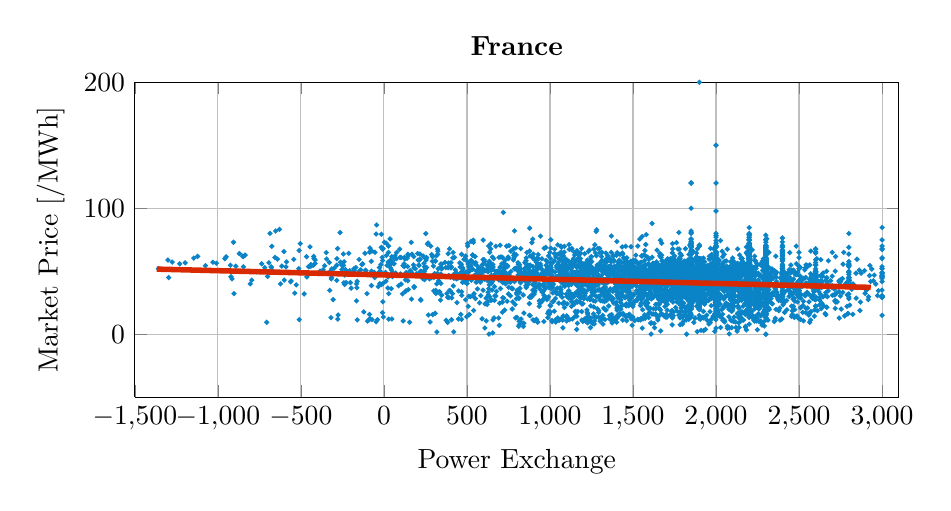
\begin{tikzpicture}

\begin{axis}[%
width=\fwidth,
height=\fheight,
at={(0\fwidth,0\fheight)},
scale only axis,
clip mode=individual,
separate axis lines,
every outer x axis line/.append style={black},
every x tick label/.append style={font=\color{black}},
xmin=-1500,
xmax=3100,
xlabel={Power Exchange},
xmajorgrids,
every outer y axis line/.append style={black},
every y tick label/.append style={font=\color{black}},
ymin=-50,
ymax=200,
ylabel={Market Price [\euro/MWh]},
ymajorgrids,
title style={font=\bfseries},
title={France}
]
\addplot [color=mycolor1,line width=1.0pt,mark size=0.3pt,only marks,mark=*,mark options={solid},forget plot]
  table[row sep=crcr]{%
1640	15.15\\
1218	12.96\\
1135	12.09\\
1332	11.7\\
1036	11.66\\
918	11.35\\
926	9.85\\
155	9.54\\
-706	9.49\\
-510	11.64\\
-278	11.94\\
-319	13.15\\
-276	15.24\\
-3	13.69\\
-84	12.43\\
-47	9.92\\
48	12.12\\
268	15.24\\
-87	15.73\\
-121	17.73\\
294	15.63\\
498	13.93\\
876	15.1\\
1307	12.95\\
1035	9.62\\
816	7.64\\
608	4.96\\
633	0.06\\
655	1.05\\
695	7.08\\
1069	12.5\\
1087	21.31\\
1435	30.44\\
1566	35.48\\
1734	33.06\\
1863	33.78\\
1798	37.97\\
1830	37.42\\
1812	36.24\\
1929	32.18\\
2158	33.56\\
1770	52.94\\
1645	66.7\\
1557	53.53\\
1688	39.54\\
1457	35.9\\
1311	35.47\\
1544	30.64\\
1371	27.4\\
1425	25.23\\
1371	15.63\\
1165	8.74\\
1192	11.28\\
1490	12.34\\
1178	26.02\\
1566	31.66\\
1816	31.96\\
1768	31.94\\
2029	30.96\\
2096	31.45\\
1909	39.05\\
1839	30.99\\
1704	30.46\\
1720	30.43\\
1807	31.12\\
2181	36.98\\
1601	34.97\\
1731	42.18\\
1467	30.39\\
1273	26.32\\
1562	31.82\\
1321	32.22\\
1906	11.94\\
2232	10.5\\
1798	7.93\\
1630	5.23\\
1556	4.86\\
1612	8.96\\
842	8.72\\
1013	9.91\\
1533	11.5\\
1873	12.76\\
1918	13.36\\
2024	14.03\\
1679	15.64\\
1983	14.24\\
2488	14.48\\
3000	30\\
2742	12.86\\
2560	16.79\\
2046	21.08\\
1924	18.1\\
1636	16.14\\
2078	13.84\\
2220	14.89\\
2413	17.34\\
2458	15.46\\
2270	14.69\\
2472	13.33\\
2355	10.96\\
2288	9.83\\
2307	11.66\\
1055	11\\
1047	11.38\\
1269	13.77\\
1696	27.42\\
1799	30.9\\
1859	32.45\\
1866	32.07\\
2052	29.91\\
2238	28.41\\
2293	16.89\\
2281	15.39\\
3000	46.14\\
2673	40.13\\
2548	38.49\\
2249	34.67\\
1866	29.4\\
1984	28.81\\
2107	22.08\\
1736	13.84\\
1377	11.89\\
1219	9.85\\
1078	5.09\\
1161	3.79\\
1267	8.24\\
2179	17.29\\
2645	48.6\\
2405	46.6\\
2623	40\\
3000	67.8\\
3000	67.3\\
3000	46.08\\
3000	46.08\\
2978	34.5\\
3000	46.08\\
3000	48.99\\
3000	84.71\\
2927	54.57\\
2456	50.7\\
2750	41.75\\
2331	28.34\\
2700	38.52\\
2472	33.69\\
1965	9.26\\
2259	9.98\\
1937	3.88\\
1823	0.07\\
1887	2.05\\
2291	6.52\\
2527	26.07\\
3000	34.99\\
2800	49.42\\
2154	52\\
1997	52\\
1760	54.36\\
1516	52.78\\
2090	49.99\\
2334	45.93\\
2581	43\\
2574	46\\
2552	54.44\\
2360	61.93\\
1646	56.29\\
2399	40.02\\
2560	31.58\\
2618	36.08\\
2414	33.51\\
2247	22.01\\
2469	14.61\\
2357	12.67\\
2227	11.34\\
2351	9.99\\
2650	22.41\\
2330	30.31\\
1174	46.42\\
2054	57.96\\
1739	57.82\\
1350	53.7\\
1418	54.51\\
1845	56.46\\
2302	54.3\\
2535	51.11\\
3000	47\\
3000	52.06\\
3000	70.01\\
2769	65\\
2233	61.89\\
2843	48.39\\
2814	38.97\\
2962	39.86\\
2637	38.79\\
2188	27.18\\
2392	26.5\\
2061	24.83\\
1841	18.34\\
1874	12.96\\
2221	25.04\\
1521	34.65\\
1211	48\\
1987	56.97\\
1749	48.54\\
1776	46.99\\
1771	47.38\\
2073	48.92\\
2262	46.65\\
2237	41.82\\
2303	37.84\\
2467	43.83\\
2132	52.66\\
1996	62.06\\
1167	59.78\\
1339	47.89\\
2323	40.66\\
2362	45.35\\
2216	44.29\\
1923	42.64\\
1703	38\\
2406	32.2\\
2564	16.27\\
2661	15.49\\
2741	33.77\\
2425	46.7\\
2142	62.87\\
2849	59.51\\
2720	61.62\\
2607	59.99\\
2677	58.32\\
2015	57.73\\
2552	53.76\\
2863	50.84\\
2953	46.87\\
3000	53.65\\
3000	74.86\\
2571	66.02\\
1883	61.5\\
1879	57.3\\
2089	46.82\\
1188	50\\
1203	47.33\\
1238	40.36\\
1382	28.17\\
1172	35.03\\
1822	28.26\\
2377	26.76\\
1973	28.27\\
1037	34.12\\
418	38.34\\
1890	43.65\\
1914	45\\
2264	46.36\\
2201	46.34\\
1783	49.72\\
2150	41.89\\
2111	37.94\\
2228	38.34\\
2513	40.28\\
2938	51.79\\
2631	59.12\\
2304	58.65\\
1830	50.94\\
2302	44.8\\
2118	52.81\\
1346	48.69\\
2333	43.47\\
1767	40\\
2116	25.86\\
2012	16.97\\
2774	14.51\\
2657	16.47\\
2793	16.18\\
2805	23.1\\
2719	31.5\\
3000	44.33\\
2188	25.75\\
2025	23.98\\
1923	29.73\\
1806	24.67\\
2560	25.7\\
2624	27.07\\
2235	31.11\\
2625	39.66\\
2364	41.96\\
2001	46.09\\
1752	37.35\\
1567	32.85\\
919	37.62\\
1125	32.17\\
1507	26\\
2464	27.86\\
2291	27.6\\
2134	13.45\\
2239	14.24\\
2247	26.71\\
1770	33.11\\
1289	50.84\\
1910	51.45\\
2110	53.89\\
2600	64.36\\
2600	65.14\\
2484	55.89\\
2600	55\\
2600	54.94\\
2600	54.97\\
2280	57.93\\
2600	67.48\\
2303	64.41\\
1463	60.71\\
1491	51.62\\
2600	44.67\\
2600	43.21\\
2600	43.21\\
1257	31.14\\
991	29.65\\
1560	29.56\\
2281	24.17\\
2361	19.72\\
2003	30.34\\
1062	36.98\\
927	60.09\\
764	65.94\\
878	66.06\\
1131	66.95\\
1264	67.51\\
1005	60.02\\
1078	55.01\\
1354	52.54\\
1598	51.86\\
1914	55.88\\
1842	70.68\\
824	68\\
511	53.7\\
591	54.94\\
1935	45.14\\
1785	44.94\\
1585	39.99\\
1761	33.03\\
1609	30.66\\
1759	29.92\\
2137	29.63\\
1993	29.54\\
1782	30.65\\
1096	39.94\\
1645	55.67\\
1401	62.65\\
1511	58.07\\
1676	55.47\\
1634	53.9\\
1245	54.16\\
1225	54.35\\
1371	50.75\\
1895	50.51\\
2219	52.1\\
2149	56.49\\
1073	62.96\\
705	61.29\\
1685	47\\
2505	38.6\\
1828	39.46\\
1334	35.75\\
1673	30.06\\
2303	28.92\\
2415	25.6\\
2242	21.42\\
2292	18.42\\
2262	28.66\\
1409	33.35\\
1694	50.09\\
1999	48.34\\
1999	51.57\\
1932	50.84\\
2027	52.2\\
2291	51.52\\
2800	55\\
2800	54.94\\
2800	53.62\\
2800	55\\
2800	79.94\\
2765	55.55\\
2542	55\\
2642	46.02\\
2433	35.23\\
2596	37.69\\
2800	38\\
2091	29.53\\
2800	28.17\\
2474	19.58\\
2313	11.23\\
2385	11.18\\
2318	20.74\\
1726	34.03\\
1784	48.97\\
1963	49.96\\
2592	47.71\\
2570	47.91\\
2428	47.96\\
2449	48.68\\
2610	46.17\\
2740	42.32\\
2800	47.44\\
2800	48.87\\
2800	68.99\\
2538	52.75\\
1894	49.43\\
2522	43.74\\
2549	33.33\\
2676	34.45\\
2107	35.9\\
2113	30.5\\
1990	29.79\\
2511	28.58\\
2719	26.79\\
2610	18.63\\
2455	22.25\\
1692	22\\
1707	30.25\\
2009	33.34\\
2397	39.96\\
2360	35.17\\
2222	32.44\\
1857	31.28\\
1928	30.89\\
2141	30.68\\
2302	30.88\\
2763	33.17\\
2800	54.53\\
2800	45.05\\
2552	39.72\\
2579	30.21\\
2326	28.63\\
2445	30.4\\
1968	38.63\\
1462	36.1\\
1407	30.14\\
2475	26.15\\
2272	9.48\\
2248	12.8\\
2304	16.41\\
1384	12.18\\
1478	15.76\\
1842	29.99\\
1965	37.57\\
2526	44.38\\
2629	46.47\\
2666	49.96\\
2761	44.12\\
2818	35.64\\
2917	27.42\\
2919	29.67\\
3000	60.71\\
3000	60\\
2925	46.54\\
2690	42.51\\
2780	40.02\\
2931	41.86\\
2611	38\\
2288	34.75\\
3000	29.46\\
3000	29.21\\
3000	14.99\\
3000	29.33\\
2721	25.5\\
2022	45.93\\
1738	71.97\\
1047	70.92\\
1436	64.5\\
1149	62.93\\
1337	64.44\\
1097	59.61\\
1696	58.04\\
1896	54.16\\
2189	49.7\\
2319	52.53\\
2319	64.91\\
1370	77.99\\
785	63.97\\
1517	62.7\\
2894	50.4\\
2285	58.17\\
2469	49.38\\
2146	44.79\\
2243	34.35\\
2973	30.65\\
3000	30.3\\
3000	30.65\\
2620	33.68\\
1778	45.86\\
1907	59.91\\
1567	62.98\\
1183	60.19\\
1043	63.32\\
1231	65.65\\
1176	62.91\\
1583	61.46\\
1411	57.41\\
1826	50.81\\
1959	54.09\\
2204	60.23\\
783	60.57\\
535	62.97\\
628	52.97\\
983	48.03\\
1080	51.45\\
1611	47.44\\
1518	45.67\\
1722	43.09\\
1634	34.97\\
1786	31.02\\
2314	31.14\\
1066	35.41\\
432	48.5\\
323	67.49\\
-511	66.49\\
-602	65.66\\
-656	60.88\\
-836	62.79\\
-950	61.44\\
-543	59.37\\
-415	58.96\\
-284	54.76\\
47	61.62\\
262	71.58\\
-686	80.06\\
-871	64.04\\
-852	62\\
-679	53.5\\
-847	61.58\\
-590	53.5\\
1322	41.81\\
1613	41.5\\
1780	39.22\\
2514	31.32\\
2711	31.17\\
1824	34.03\\
1435	43.13\\
857	60.59\\
-86	65.1\\
-54	65.05\\
77	64.92\\
146	62.17\\
257	60.92\\
715	60.91\\
977	54.77\\
1453	49.69\\
1629	48.08\\
1572	55.17\\
387	63.96\\
-240	57.53\\
897	53.78\\
2051	45.45\\
1678	53.8\\
1934	46.91\\
1206	35.05\\
1831	32.29\\
2398	30.34\\
2440	29.99\\
2538	30.53\\
1881	32.17\\
1262	43.42\\
180	61.6\\
15	62.5\\
324	63.3\\
293	61.59\\
287	63.28\\
255	60.39\\
492	59.33\\
206	58.97\\
389	53.19\\
700	53.03\\
1060	64.41\\
27	64.94\\
-244	63.71\\
211	54.64\\
1419	50.15\\
2220	47.09\\
1852	49\\
2697	37.68\\
1851	32.05\\
2168	31.1\\
2749	30.32\\
2671	29.83\\
2577	29.04\\
2701	30.9\\
1969	31.58\\
2306	39.27\\
2434	42.04\\
2563	43.63\\
2517	44.11\\
2329	45.82\\
2399	37.68\\
2230	32.69\\
2211	32.69\\
2249	33.57\\
2520	38.13\\
2323	48.04\\
2317	43.14\\
1927	32.57\\
1589	30.05\\
1814	32.86\\
1268	38.23\\
1130	22.11\\
1338	19.14\\
1359	14.85\\
1405	13.14\\
1377	13.22\\
1575	12.73\\
1401	9.53\\
1407	14.05\\
1454	14.04\\
1884	22.19\\
1971	22.69\\
1833	22.85\\
1456	23.42\\
1706	19.08\\
1472	15.23\\
1248	12.89\\
1258	8.26\\
1745	17.66\\
1354	22.42\\
1340	26.7\\
1868	31.96\\
1645	23.75\\
1966	28.24\\
2000	20.29\\
1402	12.63\\
1529	11.74\\
1649	12.81\\
1495	7.1\\
1606	8.77\\
2034	13.09\\
1853	30.14\\
1534	47.43\\
1649	51.07\\
1509	52.47\\
1338	53.47\\
1256	52.73\\
1138	56.05\\
1318	50.71\\
1357	51.92\\
1330	51.92\\
1214	51.47\\
1228	55.53\\
252	79.92\\
-114	64.25\\
953	47.25\\
1112	38.71\\
501	40.2\\
89	38.51\\
819	36.41\\
1190	32.92\\
1335	30.28\\
1647	29.57\\
1793	30.16\\
1468	31.21\\
483	41.47\\
178	55.05\\
457	56.58\\
743	54.52\\
800	52\\
727	52.44\\
515	49.94\\
1081	47.44\\
1232	46.5\\
1497	48\\
1644	49.77\\
1335	57.75\\
631	70\\
236	62.09\\
508	56.94\\
1443	47.4\\
459	53.42\\
54	48.28\\
1198	38.65\\
1424	30.54\\
1556	29.63\\
1918	28.98\\
1532	29.55\\
1306	31.08\\
182	37.1\\
-440	55.38\\
-678	52.95\\
-718	52.9\\
-587	57.44\\
-693	56.78\\
-846	53.55\\
-892	54\\
-667	50.01\\
-30	47.44\\
253	47.02\\
-466	61.52\\
-629	83.27\\
-906	72.99\\
-1075	54.43\\
-767	49.5\\
-615	54.11\\
-513	52.05\\
-34	37.75\\
597	34.94\\
450	34.29\\
1204	29.92\\
1501	30.32\\
300	34.43\\
400	45.2\\
406	53.07\\
-925	54.73\\
-347	64.78\\
-283	59.99\\
-212	64.16\\
-345	59.72\\
115	54.48\\
348	51.89\\
248	51.5\\
535	51.56\\
733	55.12\\
-279	67.98\\
-641	59.67\\
-206	50.5\\
350	45.81\\
702	46.52\\
58	47.1\\
727	42.96\\
499	42.5\\
768	36.54\\
800	33.06\\
1099	31.95\\
965	40.03\\
1006	46.9\\
282	69.94\\
-504	71.95\\
15	72.19\\
325	65.88\\
124	60.93\\
-169	52.93\\
305	48.14\\
874	45\\
833	44.1\\
1238	44.23\\
873	52.92\\
-423	61.76\\
-1009	56.35\\
-31	49.08\\
318	40\\
-161	41.99\\
-528	39.17\\
629	31.04\\
812	28.94\\
1261	26.63\\
1403	20.87\\
1286	20.18\\
1324	20.71\\
1523	26.82\\
721	28.7\\
972	37.27\\
1311	42.65\\
1418	43.28\\
1417	44.55\\
1187	48.59\\
1151	40.24\\
1017	32.87\\
1154	32.8\\
1254	33.28\\
1477	43.56\\
1131	50.02\\
1134	44.94\\
1458	41.24\\
970	35.81\\
897	35.01\\
563	35.96\\
-562	41.62\\
-480	31.96\\
-6	25.8\\
1223	19.38\\
1107	13.18\\
1231	14.07\\
987	16.54\\
540	18.85\\
508	22.07\\
469	30.83\\
750	31.96\\
905	31.82\\
908	34.15\\
1041	32.14\\
964	30.8\\
1635	31.03\\
2169	32.95\\
1661	36.15\\
1659	48.68\\
1644	54.57\\
1386	53.78\\
1216	45.76\\
817	49.81\\
53	48.84\\
422	44.37\\
182	37.8\\
938	36\\
1134	31.56\\
1058	31.52\\
631	36.19\\
298	54.1\\
504	71.89\\
3	72.94\\
-8	67.5\\
50	57.18\\
19	54.63\\
-27	52.9\\
326	51.96\\
647	46.82\\
906	47.14\\
1098	46.76\\
1190	54.09\\
395	67.8\\
75	59.96\\
1158	57.98\\
1838	48.72\\
1251	52.2\\
718	52.27\\
1076	44.42\\
286	44.96\\
716	40.9\\
1210	30.63\\
1145	30\\
379	32.38\\
29	47.13\\
139	60.3\\
-8	58.49\\
404	53.88\\
948	51.99\\
1007	52.83\\
621	54.68\\
993	51.68\\
1349	48.05\\
1447	47.59\\
1614	48.03\\
1847	53.05\\
1027	63.99\\
507	55.73\\
987	48\\
2055	41.26\\
1689	44.08\\
1313	42.46\\
762	30.53\\
511	29.98\\
1187	28.99\\
1701	25.71\\
1733	18.11\\
1557	28.08\\
953	33.51\\
1012	45.16\\
1070	49.94\\
1041	52.61\\
1313	58.57\\
1306	54.16\\
1064	48.08\\
1233	52.2\\
1327	50.09\\
1915	43.92\\
2099	42.55\\
2049	49.69\\
1116	67.38\\
651	53.32\\
1323	36.79\\
-1030	57.1\\
-1358	52\\
-1296	45\\
-559	42.28\\
-623	39.94\\
-326	34.79\\
551	28.27\\
615	28.67\\
-903	32.2\\
-915	44\\
-1230	55.87\\
-1197	56.7\\
-1301	58.84\\
-1122	61.77\\
-1145	60.43\\
-1275	57.28\\
-736	55.91\\
-18	55.29\\
157	49.94\\
670	47.89\\
639	55.89\\
-72	66.01\\
-958	60.02\\
-396	48.05\\
993	37.12\\
1063	33.71\\
895	39.61\\
1657	23.64\\
2034	19.51\\
1743	14.66\\
1560	12.18\\
1627	8.54\\
1588	15.42\\
1906	30.68\\
1560	47.79\\
1691	45.71\\
1956	47.63\\
2201	47.94\\
2441	51.34\\
2217	48.37\\
2255	42.94\\
2252	36.86\\
2232	32.31\\
2317	31.3\\
2606	36.16\\
2285	59.92\\
1969	54.71\\
2077	43.31\\
1778	30.49\\
2265	38.37\\
2310	40.84\\
1726	28\\
1160	26.43\\
1670	25.9\\
1383	24.93\\
1268	10.52\\
1262	16.2\\
1474	24.04\\
649	27.13\\
889	29.51\\
1241	29.48\\
1591	28.07\\
1671	26.76\\
1611	28.03\\
1693	25.5\\
1577	25.96\\
2287	28.81\\
2088	28.03\\
1612	31.17\\
1656	42.58\\
1379	33.88\\
982	27.57\\
1077	24.29\\
1241	27.55\\
1636	23.6\\
1162	14.23\\
663	13.02\\
691	12.87\\
467	11.77\\
278	9.72\\
384	9.36\\
616	10.63\\
116	10.54\\
375	11.04\\
727	19.16\\
1002	17.7\\
1225	17.29\\
1463	14.68\\
1595	13.16\\
1376	10.5\\
1374	8.97\\
1319	12.42\\
1416	14.69\\
1805	35.79\\
1541	36.81\\
1593	31.23\\
1241	27.97\\
1278	30.04\\
1916	25.31\\
775	36.13\\
1215	33.87\\
1887	27.22\\
1931	23.86\\
1001	23.08\\
1188	33.18\\
25	45.43\\
482	59.42\\
425	60.99\\
213	58.79\\
-421	60.02\\
-254	54.96\\
-414	56.12\\
404	56.82\\
343	55.63\\
601	51.47\\
967	47.44\\
924	54.94\\
-47	79.49\\
-357	54.32\\
-75	50.06\\
821	46.57\\
753	47.59\\
1349	42.83\\
1762	30.75\\
1705	32.07\\
1467	29.45\\
1922	28.27\\
2226	28.05\\
1641	30.72\\
761	41.12\\
646	53.8\\
643	55.34\\
1003	56.62\\
1003	54.1\\
923	51.74\\
614	50.38\\
880	49.25\\
1493	42.49\\
1768	39.56\\
1560	41\\
786	51.9\\
604	58.97\\
95	67.49\\
244	50\\
1152	46.48\\
627	49.48\\
760	44.09\\
764	45\\
749	41.94\\
666	37.84\\
813	28.43\\
880	29.36\\
24	36.72\\
-464	45.54\\
-149	59.3\\
-82	65.77\\
-84	68.42\\
103	60.87\\
-128	55.9\\
-147	50.33\\
505	49.42\\
848	45.92\\
1165	43.34\\
1721	40.93\\
1049	44.99\\
254	58.94\\
-436	54.37\\
189	52.03\\
1429	42.78\\
483	46.13\\
437	44.03\\
693	42.97\\
909	34.54\\
1071	32.23\\
1838	18.33\\
1899	12.47\\
1304	26.67\\
980	42.44\\
122	55.88\\
244	53.54\\
606	57.79\\
1016	56.72\\
1459	57.98\\
1284	55\\
1772	52.89\\
1771	52.35\\
2186	45.25\\
2803	42.91\\
2121	48.66\\
975	68.92\\
730	58.69\\
1662	52.81\\
1786	42\\
2049	40.63\\
1272	38.04\\
2455	33\\
2347	32.72\\
2141	29.33\\
2638	24.42\\
2730	25.63\\
2243	29.44\\
1474	46.4\\
1615	61.12\\
1149	64.8\\
1435	69.25\\
1751	62.12\\
1702	55\\
1793	52.08\\
2397	47.1\\
2421	44.22\\
2480	36.2\\
2516	40\\
2420	46.18\\
1643	53.48\\
1661	48.73\\
2356	36.97\\
2095	30.39\\
2657	30.61\\
2948	42.44\\
1654	27.73\\
1191	17.99\\
1549	12.38\\
1302	10.36\\
1198	10.11\\
1244	10.33\\
1544	11.36\\
801	13.34\\
1026	18.26\\
1004	22.66\\
1436	23.11\\
1402	23.08\\
1145	23.76\\
1246	22.48\\
1594	21.11\\
1665	19.33\\
1658	20.46\\
1550	27.73\\
1591	39.29\\
1277	44.85\\
1131	28.93\\
1073	29.36\\
1193	41.5\\
1207	41.56\\
1401	25.49\\
1101	14.46\\
1379	12.35\\
1228	9.06\\
1244	5.3\\
1319	8.08\\
1388	11.12\\
926	9.53\\
904	10.73\\
1100	13.37\\
1159	16.81\\
1153	17.86\\
992	18.23\\
987	13.15\\
898	11.38\\
1100	10.48\\
1359	12.22\\
1723	15.26\\
2119	40.15\\
2214	47.98\\
2134	46.83\\
2047	34.73\\
2368	39.08\\
2487	31.53\\
2157	31.59\\
2491	25.69\\
2404	23.33\\
2290	17.52\\
2321	19.63\\
2715	26.47\\
1814	43.79\\
1503	58.75\\
1737	53.31\\
1954	54\\
2018	49.32\\
1989	50\\
1975	44.22\\
2450	42.07\\
2485	34.96\\
2816	37.25\\
2057	40.33\\
2080	43.03\\
786	82.04\\
643	71.74\\
388	56.51\\
1011	47.19\\
674	49.94\\
1333	43.43\\
1530	31.95\\
1780	31.66\\
1537	30.09\\
1488	28.86\\
1623	29.2\\
1324	31.3\\
824	42.03\\
-252	56.19\\
-424	54.9\\
-444	53.79\\
-314	51.9\\
-112	50.74\\
-253	51.42\\
51	48.48\\
785	43.27\\
1051	43.44\\
1196	45.72\\
1417	53.91\\
525	73.68\\
63	59.98\\
906	45.94\\
2081	39.68\\
1756	41.9\\
1590	36.47\\
1784	32.16\\
1840	29.65\\
1962	28.46\\
2266	27.67\\
2472	28.51\\
1538	29.34\\
1496	38.19\\
961	47.45\\
1164	49.44\\
1544	52.21\\
1475	53.93\\
1669	53.96\\
1361	50.76\\
1859	49.48\\
1781	49.37\\
1826	47.95\\
2021	44.71\\
1743	47.44\\
504	70\\
218	59.54\\
524	54.27\\
1741	47.02\\
2417	44.18\\
1727	44.96\\
1577	31.28\\
1916	29.47\\
2211	28.87\\
2016	27.75\\
2318	25.59\\
1226	27.85\\
1113	34.51\\
1064	46.28\\
953	48.34\\
1346	48.28\\
2074	44.93\\
2193	46.95\\
1932	47.58\\
2667	44.94\\
2825	40.02\\
2906	34.96\\
2898	32.45\\
3000	41.78\\
2565	55\\
2242	52.17\\
2357	47.44\\
2323	39.95\\
2667	41.78\\
2565	41.49\\
2727	32.91\\
2789	22.15\\
2552	20.84\\
2427	19.42\\
2509	21.02\\
1935	26.64\\
2712	35.83\\
2506	46.31\\
2436	49.03\\
2508	52.95\\
2718	50.07\\
2874	48.45\\
2518	42.88\\
2665	37.61\\
2544	32.16\\
2556	32.1\\
2628	31.68\\
2594	42.9\\
2493	49.44\\
1437	49.96\\
1998	49.08\\
1848	40.71\\
1740	40.93\\
1294	41\\
652	35.11\\
522	29.96\\
952	26.09\\
1848	21.02\\
1763	18.67\\
1757	21.15\\
1526	27.93\\
876	29.38\\
1570	32.92\\
2002	37.43\\
2305	37.35\\
2446	36.86\\
2372	38.85\\
2198	35.47\\
2172	29.59\\
2021	31.99\\
1987	31.33\\
2247	37.71\\
2124	50.91\\
1957	53.1\\
1578	44.22\\
1591	36.72\\
1324	40.34\\
1393	36.96\\
1837	26.11\\
1264	21.63\\
1499	22.07\\
1558	19.48\\
1441	16.28\\
1427	19.86\\
1420	15.73\\
463	15.73\\
-8	17.1\\
309	16.63\\
713	17.46\\
843	16.77\\
880	14.68\\
1783	12.98\\
1650	11.26\\
1736	7.45\\
1511	10.84\\
1438	11.28\\
1779	24.31\\
1875	35.49\\
2004	27.81\\
1799	23.11\\
1925	27.1\\
1861	25.71\\
1361	14.5\\
1816	15.09\\
1598	17.22\\
1499	13.68\\
1568	14\\
1167	18.12\\
1233	35.66\\
1402	46.95\\
1348	50\\
1837	46.65\\
1978	45.98\\
1853	41.79\\
1426	40.46\\
1979	39.32\\
2233	35.99\\
2457	31.07\\
2661	32.97\\
2700	46.16\\
2700	64.95\\
2444	64.73\\
2223	48.99\\
1987	35.43\\
1871	37.44\\
1435	33.87\\
742	26.22\\
1193	23.87\\
1472	22.77\\
1638	20.29\\
1735	18.97\\
1328	25.94\\
857	36.97\\
945	46.95\\
1054	46.66\\
1603	46.12\\
1353	44.59\\
1385	44\\
1574	44.94\\
2023	40.49\\
2201	36.09\\
2477	35.3\\
2590	33.71\\
2423	42.61\\
1762	72.68\\
1792	62.52\\
1382	46.87\\
2007	39.88\\
1345	42.89\\
1080	39.59\\
1732	36.05\\
1820	30\\
1705	27.29\\
1480	26.91\\
1528	27.86\\
1033	28.48\\
1471	39.22\\
909	45.05\\
1391	49.24\\
2166	51.3\\
2353	50.42\\
2092	50\\
1957	46.91\\
1962	46.42\\
1998	44.96\\
1960	43.35\\
1842	41.81\\
1536	43.99\\
1115	71.19\\
539	72.95\\
224	49.85\\
580	45.59\\
1179	42.44\\
1262	40.05\\
1319	33.99\\
1430	32.03\\
1137	30.28\\
970	29.61\\
973	29.48\\
413	32.18\\
1074	41.54\\
1060	53.34\\
718	50.1\\
1290	47.1\\
1285	48.14\\
929	46\\
1101	44.24\\
1290	44.81\\
1389	43.22\\
1826	41.94\\
2088	40.62\\
1477	51.76\\
1369	64.96\\
1772	57.83\\
1784	48.66\\
1977	43.21\\
1947	41.45\\
1845	40.16\\
1575	36.25\\
1803	34.94\\
1757	30.19\\
1785	28.03\\
1709	28.54\\
1102	29.94\\
1718	39.6\\
1235	47.45\\
1853	49.45\\
2032	49.77\\
2366	49.12\\
2477	47.42\\
2635	46.72\\
2667	44.7\\
2637	42.31\\
2618	41.92\\
2579	42.98\\
2487	47.3\\
1405	64.68\\
951	59.92\\
1561	47.28\\
1625	39.75\\
1246	42.95\\
997	42\\
1191	40.61\\
1190	35.72\\
1186	33.79\\
1171	30.22\\
1331	29.28\\
1351	29.33\\
715	28.98\\
1027	33.71\\
1129	39.51\\
1228	47.4\\
1510	50.34\\
1524	48.18\\
1737	47.97\\
1787	43.25\\
1672	38.63\\
1629	36.46\\
1527	33.77\\
1346	41.27\\
929	63.21\\
598	74.76\\
837	45.93\\
905	42.66\\
167	48.38\\
460	44.97\\
-55	44.94\\
-14	39.4\\
29	32.28\\
384	29.31\\
221	27.57\\
166	27.86\\
492	27.33\\
341	27.04\\
-306	27.49\\
313	32.39\\
336	33.69\\
468	33.67\\
399	34.38\\
957	27.45\\
790	23.55\\
697	24.59\\
713	25.42\\
798	28.22\\
678	33.96\\
575	42.62\\
1273	39.44\\
799	31.89\\
44	36.16\\
-537	32.59\\
-165	26.52\\
440	25.11\\
609	24.08\\
936	22.14\\
1104	24.03\\
222	27.01\\
-317	43.93\\
-226	49.94\\
-232	51.33\\
123	53.68\\
514	51.43\\
636	57.13\\
459	47.83\\
598	49.41\\
735	46.48\\
1626	38.95\\
1481	40.98\\
1434	44.96\\
165	72.91\\
-264	80.69\\
99	47.81\\
275	43.99\\
258	45.3\\
498	43.34\\
301	45.03\\
634	39.19\\
955	33.29\\
1293	28.99\\
1447	29.68\\
818	33.28\\
-78	47.18\\
565	53.9\\
-76	57.9\\
25	57.32\\
-140	51.02\\
-181	51.98\\
-300	52.3\\
-22	50\\
71	48.59\\
439	46.51\\
749	45.92\\
956	45.87\\
37	75.64\\
-15	79.38\\
28	54.77\\
620	50.68\\
167	49.01\\
-180	50.54\\
343	40.21\\
-165	39.94\\
12	42.1\\
312	34.72\\
628	33.37\\
555	41.28\\
326	47.32\\
991	62.16\\
780	67.76\\
1288	68.08\\
1488	53.01\\
1480	44.96\\
1392	43.85\\
1176	44.19\\
2080	40.21\\
2391	38.02\\
2516	38.08\\
1769	46.54\\
1100	58.03\\
1005	68.37\\
1797	49.04\\
2065	42.58\\
1451	45.99\\
1021	44.1\\
1233	37.43\\
1238	36.72\\
958	34.14\\
1296	28.81\\
1372	29.19\\
1311	33.98\\
723	42.85\\
-132	55.33\\
-329	56.97\\
241	56.22\\
1056	50\\
968	48.58\\
549	46.41\\
826	44.92\\
1666	40.51\\
2070	34.11\\
2138	37\\
1604	45\\
238	61.59\\
-675	69.75\\
466	53.9\\
1005	42.17\\
52	45.73\\
-202	40.97\\
-805	40.01\\
130	33.98\\
-102	32.22\\
408	28.9\\
391	29.1\\
112	32.06\\
-241	40.9\\
-250	48.26\\
143	53.76\\
492	62\\
1180	49.17\\
967	45.36\\
899	44.82\\
1186	37.93\\
1298	35.64\\
1661	31.97\\
1838	31.94\\
1953	39.36\\
1396	47.09\\
1468	49.26\\
1845	45.95\\
1525	41.92\\
1067	44.28\\
1061	43.68\\
1019	39.97\\
906	33.31\\
537	30.44\\
776	25.71\\
576	24.96\\
625	25.82\\
666	26.92\\
637	29.6\\
1259	31.96\\
1354	31.51\\
1204	28.19\\
1022	26.17\\
939	24.42\\
773	20.02\\
997	15.91\\
1208	12.03\\
1621	16.02\\
2068	22.55\\
2063	35.58\\
1697	42.77\\
1293	30.03\\
1138	25.14\\
1084	25.47\\
622	23.65\\
514	15.67\\
1148	13.75\\
826	12.1\\
657	11.4\\
-99	10.35\\
-90	11.4\\
407	11.49\\
-161	11.4\\
-72	11.55\\
29	12.05\\
-39	11.54\\
449	12.11\\
591	12.26\\
814	10.29\\
840	6.2\\
319	1.75\\
420	1.87\\
822	9.83\\
1459	22.41\\
1755	41.73\\
1658	34.86\\
1366	28.07\\
1421	30.09\\
643	26.92\\
1199	24.26\\
1580	22.62\\
1474	22.73\\
1545	22.76\\
1808	22.11\\
1166	25.57\\
1594	43.5\\
1910	48.28\\
1927	48.12\\
1765	44.76\\
1766	40.9\\
1604	37.42\\
1477	36.46\\
1573	35.85\\
1641	33.8\\
1832	30.13\\
2058	30.19\\
2356	36.36\\
1711	56.07\\
896	75.46\\
867	46.32\\
1707	38.68\\
1474	35.17\\
1118	30.93\\
1017	25.83\\
1130	25.9\\
1053	24.63\\
1572	24.27\\
1707	23.78\\
936	26.5\\
1287	35.08\\
1804	42.55\\
1888	44.58\\
1844	40.03\\
2416	40.2\\
2274	36.07\\
1920	31.88\\
1846	30.65\\
2024	28.18\\
2156	28.72\\
2293	30.91\\
2584	36.26\\
2600	49.94\\
2141	54.1\\
2459	42.56\\
2110	34.04\\
1826	40.03\\
1764	32.99\\
1490	28.87\\
1697	28.04\\
1517	26.65\\
1793	25.15\\
1764	25.69\\
1733	28.09\\
2267	35.8\\
1875	44.54\\
1717	43.73\\
2206	41.27\\
1953	32.59\\
1730	33.67\\
1591	30\\
1661	28.78\\
1863	28.42\\
2092	29.25\\
2277	30.79\\
2700	37.04\\
2415	49\\
2304	75.98\\
2254	48.43\\
2217	42.01\\
2477	38.28\\
2448	32.08\\
2533	31.35\\
1629	30.65\\
2197	29.96\\
2010	30\\
1885	30.11\\
1665	31.43\\
2749	43.03\\
2115	53.46\\
2292	49.84\\
1842	41.27\\
1801	34.74\\
1553	29.77\\
1328	30.58\\
1370	28.42\\
1410	28.78\\
1561	30.95\\
1693	35.54\\
1968	30.84\\
1485	52.76\\
1541	75.55\\
1596	48.69\\
2294	43.63\\
2662	42.87\\
2542	40.69\\
2177	34.96\\
2324	32.01\\
2583	30.99\\
2498	29.57\\
2644	29.65\\
1885	32.89\\
2585	42.04\\
1534	49.94\\
2158	47.93\\
2236	42.94\\
2788	41.26\\
2592	38.83\\
2313	37.01\\
2289	34.91\\
2182	30.96\\
2279	29.53\\
2374	30.91\\
2640	37.91\\
2445	45.07\\
1965	53.95\\
2800	49.94\\
2796	38.64\\
2800	42.44\\
2800	38.99\\
1776	28.64\\
1818	18.86\\
1837	21.1\\
1820	11.3\\
1784	7.58\\
1836	11.81\\
1847	13.36\\
1937	14.02\\
2271	22.83\\
2754	20.01\\
2795	16.52\\
2824	15.8\\
2667	21.57\\
2558	15.2\\
2497	12.55\\
2508	11.78\\
2570	11.26\\
2867	18.81\\
3000	44.94\\
3000	48\\
2870	25.54\\
2623	23.29\\
2634	20.33\\
2378	19.29\\
2040	15.89\\
2455	14.23\\
2149	13.29\\
1972	11.77\\
2050	11.11\\
963	10.12\\
1076	11.23\\
1012	10.91\\
1239	11.44\\
1462	10.77\\
1550	12.34\\
1568	13.02\\
1481	13.95\\
1947	11.07\\
1866	9.33\\
1910	3.07\\
2139	5.41\\
2564	9.43\\
2523	22.78\\
3000	52\\
3000	49\\
2667	21.31\\
2718	20.51\\
2844	28.62\\
2312	29.73\\
1916	26.33\\
2057	23.93\\
2540	20.73\\
2600	21.96\\
1837	26.41\\
2600	42\\
2467	50.81\\
2122	49\\
2600	56.84\\
2600	59.16\\
2600	65.27\\
2600	50\\
2600	50\\
2600	49.96\\
2600	49.08\\
2600	51.87\\
2600	67.78\\
2600	47.44\\
2483	69.94\\
2451	54.86\\
2600	44\\
2600	45\\
2600	44.25\\
2400	31.57\\
2400	32.18\\
2400	29.99\\
2340	24.07\\
2103	24.89\\
2372	28.06\\
2139	40.44\\
2400	49.49\\
2400	50.12\\
2400	63.77\\
2400	55\\
2400	61.99\\
2400	58.13\\
2400	52.24\\
2400	45.13\\
2400	42\\
2400	41.36\\
2400	42.44\\
2400	39.68\\
1405	46.28\\
1675	41.55\\
2400	39\\
2340	32.73\\
2313	30.33\\
2465	22.2\\
2600	22.46\\
2593	14.3\\
2600	22.46\\
2600	29.66\\
2600	27.44\\
2600	42.36\\
2600	49.79\\
2600	47.99\\
2600	48\\
2600	39.01\\
2590	34.72\\
2365	33.41\\
2313	32.59\\
2284	31.48\\
2584	28.19\\
2600	42.44\\
2600	47.59\\
2600	42.44\\
2600	54.97\\
2600	49\\
2600	45\\
2600	44\\
2600	41.93\\
1868	26.47\\
1932	26.72\\
2335	24.54\\
2541	17.18\\
2572	18.05\\
2257	24.57\\
1620	37.54\\
1785	46.15\\
2257	41.33\\
2318	35.3\\
2344	31.3\\
2287	29.01\\
1956	26.8\\
1922	26.56\\
1940	25.76\\
2251	26.52\\
2425	26.84\\
2624	28.95\\
2465	36.94\\
2540	45.07\\
2800	32\\
2592	27.84\\
2790	31.24\\
2246	30.47\\
2265	21.24\\
2396	12.08\\
2236	11.32\\
2267	10.25\\
2527	10.65\\
2379	18.63\\
2800	29.62\\
2800	40\\
2800	39.18\\
2674	38.33\\
2800	44.54\\
2800	63.62\\
2800	57.66\\
2800	55.89\\
2800	45\\
2800	39.96\\
2800	39.94\\
2800	38.93\\
1633	42.43\\
1611	55\\
1441	47.39\\
1549	43.08\\
1328	43.08\\
772	36.5\\
1339	33.94\\
1114	28.54\\
1459	24.08\\
2204	19.07\\
2109	13.66\\
1964	17.92\\
1496	22.76\\
876	24.31\\
1178	29.83\\
1417	32.37\\
1883	32.33\\
1906	32.48\\
1945	31.22\\
2087	27.59\\
1995	27.84\\
1863	26.45\\
1765	27.99\\
2086	31.39\\
1660	38.04\\
1256	45.01\\
1642	36.93\\
1793	31.7\\
1661	30.99\\
1549	24.69\\
1788	22.91\\
1605	20.54\\
1624	20.14\\
1790	20.59\\
2148	17.65\\
2078	19.82\\
1814	17.05\\
1435	16.07\\
1418	21.36\\
1577	24.42\\
1691	26.9\\
1770	30.58\\
1737	29.26\\
2172	24.04\\
2227	23.46\\
2460	18.55\\
2522	17.34\\
2595	19.29\\
2800	40\\
2800	45.12\\
2800	42\\
2636	37.1\\
1945	40.51\\
2111	35.55\\
1737	32.64\\
2061	30\\
1934	27.8\\
1995	25.08\\
1934	25.3\\
1982	28.82\\
2200	40.58\\
2200	57.32\\
1808	57.52\\
1965	54.94\\
2115	42.91\\
2075	42.6\\
1641	43.18\\
1537	44.64\\
1648	43.91\\
1961	41.46\\
2453	40.91\\
2800	40.93\\
1160	47.23\\
719	96.69\\
1857	48.73\\
2744	41.12\\
2388	44.62\\
2640	41.69\\
751	37.3\\
-163	36.95\\
329	33.3\\
583	30.65\\
348	31\\
147	35.52\\
144	42.44\\
-315	45\\
-326	49.47\\
-385	49.99\\
-366	51.15\\
-701	45.85\\
-921	45.62\\
-796	42.97\\
-600	42.92\\
104	39.82\\
-25	40.1\\
234	44.07\\
-58	49.08\\
-652	81.94\\
198	48.12\\
244	43.42\\
-284	42.8\\
-236	46.99\\
-237	39.53\\
-227	41.02\\
-5	40.42\\
543	32.22\\
839	31.13\\
394	34.68\\
445	44.49\\
134	48.93\\
633	52.06\\
870	52.07\\
1085	54.01\\
1133	48.32\\
808	47\\
1173	43.52\\
1250	41.95\\
1626	41.09\\
1831	40.24\\
1631	42.24\\
588	48.68\\
-44	86.74\\
314	46.5\\
1334	42.37\\
605	43.59\\
329	42.44\\
2081	41.11\\
1851	42.44\\
2183	38.41\\
2287	35.02\\
2442	34.24\\
1520	38.08\\
2044	46.51\\
2083	51.57\\
1967	59.9\\
1853	52.44\\
2155	51.19\\
2034	50.58\\
1649	48.79\\
1651	49.4\\
1688	46.77\\
1973	43.27\\
2151	42.07\\
2345	44.45\\
1778	50\\
1278	81.51\\
1280	62.32\\
1187	46.92\\
1786	48.57\\
2118	45.4\\
1829	40.77\\
1247	41.97\\
1940	41.04\\
2028	37.01\\
2194	35.1\\
2492	40.21\\
2072	45.87\\
1677	51.76\\
1720	58.1\\
1642	57.39\\
1742	47.4\\
1774	45\\
2430	42.06\\
2485	40.59\\
2601	40.81\\
2800	39.99\\
2800	40\\
2800	43\\
2205	44.29\\
1529	70\\
1877	45\\
2800	42.44\\
2630	42.44\\
2299	40.06\\
2300	43.99\\
2257	32.81\\
2295	31.02\\
2300	31.11\\
2300	32\\
2300	31.32\\
2300	36.89\\
2300	39.94\\
2300	43\\
2300	47.44\\
2300	45.62\\
2300	42.62\\
2300	40\\
2300	38\\
2300	34.99\\
2300	34.96\\
2300	39.96\\
2300	43\\
2300	43\\
2300	46.17\\
2300	54.96\\
2300	46\\
2300	44.94\\
2300	40.56\\
1850	44\\
1850	34.94\\
1850	29.49\\
1850	29.49\\
1850	30.7\\
1850	35.04\\
1850	35.04\\
1850	39.33\\
1850	40\\
1850	41\\
1850	38.83\\
1850	37.44\\
1850	36.99\\
1850	32.44\\
1850	30.81\\
1850	31.8\\
1850	39.96\\
1850	39.96\\
1850	45\\
1850	69.97\\
1850	59.94\\
1850	55\\
1850	42.44\\
1180	30.91\\
1850	32.46\\
1850	31.28\\
1850	32.2\\
1850	35.77\\
1850	28.14\\
1850	40.69\\
1850	69.53\\
1850	55.47\\
1459	56.01\\
1361	48.33\\
1355	46.08\\
1291	46.7\\
1695	43.73\\
1647	41.79\\
1850	40\\
1850	42.22\\
1850	43.22\\
1850	40.47\\
1659	48.47\\
1850	54.61\\
1850	50\\
1850	44.94\\
1850	44\\
1850	54.48\\
1850	43.64\\
1850	41.06\\
1850	40.5\\
1850	36.26\\
1850	44.94\\
1850	48\\
1850	57.44\\
1662	62.19\\
1386	57.89\\
1643	47.29\\
1592	46.64\\
1791	37.77\\
1850	40\\
1850	39.96\\
1850	38.76\\
1850	39.96\\
1850	42.11\\
1850	73.81\\
1850	50.12\\
1850	45\\
1850	47\\
1850	120\\
1850	120\\
1850	65\\
1850	37.69\\
1850	37.53\\
1850	37.53\\
1850	37.75\\
1850	36.93\\
1850	44\\
1850	49.22\\
1380	62.17\\
1406	54.35\\
1850	48\\
1850	45\\
1850	45\\
1850	44\\
1850	42.12\\
1850	41.19\\
1850	44\\
1850	47.44\\
1850	46\\
1850	52.92\\
1850	58.31\\
1850	53.12\\
1850	44.94\\
1315	40.98\\
1850	34.99\\
1850	31.27\\
1850	31.27\\
1850	32.81\\
1850	28.3\\
1850	29.55\\
1850	38.64\\
1850	55.5\\
1850	52.09\\
1850	49.94\\
1850	50\\
1850	51\\
1850	47.44\\
1850	47\\
1850	44.94\\
1850	44.42\\
1850	45\\
1850	50\\
1850	69.97\\
1850	44.94\\
1850	50\\
1850	47.44\\
1850	63.41\\
1850	64.08\\
1437	37.23\\
1850	34.37\\
1850	34.24\\
1850	30.51\\
1850	30.51\\
1850	31.4\\
1850	37.77\\
1612	46.07\\
1796	51.91\\
1813	56.15\\
1850	63.46\\
1850	120\\
1850	58.9\\
1850	47.44\\
1850	44.94\\
1850	40\\
1850	40\\
1850	40\\
1850	39.94\\
1751	40.99\\
1707	41.76\\
1735	38.72\\
1850	65.37\\
1850	43\\
1850	34.3\\
1850	37.84\\
1850	34\\
1850	34\\
1850	30.74\\
1850	30.74\\
1850	29.5\\
1850	34.44\\
1850	43.18\\
1850	46\\
1850	45\\
1850	47.44\\
1850	42.8\\
1850	35.87\\
1850	34.44\\
1850	34.44\\
1850	33.61\\
1850	35\\
1850	42.44\\
1850	42.44\\
1850	49.99\\
1850	47.44\\
1850	42\\
1850	44.01\\
1850	35.16\\
1850	42.16\\
1850	34.94\\
1850	34.21\\
1850	31.5\\
1850	33.97\\
1850	24.25\\
1850	24.3\\
1850	25.31\\
1850	34.94\\
1850	38.99\\
1850	41.96\\
1850	47.44\\
1850	39.94\\
1850	35.15\\
1850	34.9\\
1850	34.94\\
1850	39.96\\
1850	42.17\\
1850	44.94\\
1850	59.94\\
1850	54.96\\
1850	48\\
1850	35.99\\
1850	29.88\\
1850	27.73\\
1850	28.85\\
1850	29.85\\
1850	29.75\\
1850	29.99\\
1850	41\\
1828	49.94\\
1781	53.05\\
1850	51.06\\
1850	47.45\\
1850	44.61\\
1850	38.94\\
1786	37.09\\
1850	36.16\\
1850	36.26\\
1850	36.31\\
1850	39.12\\
1850	45.31\\
1850	46.99\\
1850	48.75\\
1850	38.58\\
1850	34.86\\
1850	30.07\\
1850	28.01\\
1850	28.01\\
1850	21.92\\
1850	21.44\\
1850	22.69\\
1850	24.02\\
1749	31.84\\
1842	38.99\\
1683	43.96\\
1488	45.8\\
1580	48.41\\
1696	53.7\\
1493	43.88\\
1353	44.6\\
1006	45.32\\
1615	40.42\\
1850	39.94\\
1850	44.46\\
1830	39.94\\
1850	39.96\\
1850	66.56\\
1850	63.54\\
1850	65.06\\
1850	55\\
1676	41.06\\
1850	37.77\\
1850	35.97\\
1850	35.74\\
1850	37.06\\
1850	73.11\\
1850	80.78\\
1783	50.12\\
1592	55.91\\
1725	59.81\\
1850	52.44\\
1850	47.12\\
1850	44\\
1774	44.8\\
1568	41.22\\
1850	42.98\\
1850	42.99\\
1850	45.87\\
1850	55\\
1850	50.12\\
1850	54.25\\
1850	42.44\\
1850	42.44\\
1850	70\\
1850	81.93\\
1850	39.75\\
1850	60.01\\
1850	39.15\\
1850	38.88\\
1850	38.44\\
1850	69.9\\
1850	59.94\\
1784	63.98\\
1669	60.89\\
1850	54.91\\
1850	60\\
1850	45\\
1850	44.94\\
1850	72.04\\
1850	71.86\\
1850	69.9\\
1850	75.33\\
1850	75.67\\
1850	50\\
1850	50\\
1850	55\\
1850	69.9\\
1850	39.78\\
1850	50\\
1850	100\\
1850	55\\
1850	40.1\\
1850	59.94\\
1850	37.34\\
1850	42.91\\
1850	65\\
1850	70.93\\
1850	69.71\\
1850	69.54\\
1850	52.44\\
1850	68.76\\
1850	50\\
1850	42.86\\
1850	39.99\\
1850	38\\
1850	39.94\\
1850	39.94\\
1850	44.44\\
1850	42.91\\
1850	42.5\\
1850	45\\
1850	42.02\\
1850	79.9\\
1850	41.06\\
1850	39.05\\
1850	39\\
1850	38.27\\
1850	39.3\\
1850	39.54\\
1850	42.44\\
1850	46.24\\
1850	50.4\\
1850	60.52\\
1850	56.09\\
1850	45.12\\
1850	40\\
1850	38.97\\
1850	37.84\\
1850	37.66\\
1850	39.94\\
1850	42.44\\
1850	42.44\\
1850	44.94\\
1850	53.12\\
1850	50.31\\
1850	50\\
1850	40.88\\
1850	30\\
1850	19.99\\
1850	30\\
1850	34.61\\
1850	33.86\\
1850	34.92\\
1850	34.99\\
1850	39.65\\
1850	40.86\\
1850	39.94\\
1850	39.96\\
1850	39.99\\
1850	38.38\\
1850	35\\
1850	32.96\\
1850	34.94\\
1850	38.37\\
1850	41.55\\
1850	42.44\\
1850	49.96\\
1850	48\\
1850	40\\
1850	31.42\\
1850	20.12\\
1809	14.94\\
1850	14.92\\
1850	15.78\\
1850	19.96\\
1850	22.54\\
1850	37.14\\
1850	43.2\\
1197	44.35\\
1097	48.65\\
1483	48.66\\
1538	46.67\\
1476	42.9\\
1850	42.44\\
1850	45\\
1850	44.96\\
1850	44.96\\
1850	55.74\\
1850	48\\
1850	48\\
1850	50\\
1850	55\\
1850	49.04\\
1850	42.44\\
1850	38.11\\
1850	36.22\\
1850	34.31\\
1850	30\\
1850	29.27\\
1850	27.44\\
1820	38.07\\
1604	44.28\\
1758	50.97\\
1740	58.5\\
1850	51\\
1850	50.12\\
1850	47.44\\
1850	49.94\\
1850	48.66\\
1850	43\\
1850	41.33\\
1850	41.06\\
1850	40\\
1850	40\\
1850	42.32\\
1850	45\\
1850	45\\
1850	42.14\\
1779	36.96\\
1693	34.48\\
1850	33.9\\
1850	33.94\\
1850	35.15\\
1850	37.36\\
1850	40.92\\
1850	55.1\\
1384	58.87\\
1209	63.9\\
1795	47\\
1850	42.44\\
1847	39.94\\
1850	39.47\\
1850	39.94\\
1850	42\\
1850	44\\
1850	49.31\\
1850	45\\
1850	44.94\\
1850	47.44\\
1850	46.73\\
1850	72.29\\
1850	42.39\\
1850	37.73\\
1850	35.49\\
1850	34.99\\
1850	33.04\\
1850	29.25\\
1850	31.76\\
1850	38.36\\
1540	46.11\\
1438	51.52\\
1850	50\\
1850	49.94\\
1850	55.02\\
1850	44.94\\
1850	45\\
1850	42.44\\
1850	42.13\\
1850	42.44\\
1850	42.44\\
1850	39.99\\
1850	47.44\\
1850	47.44\\
1850	54.25\\
1850	45\\
1850	41.45\\
1850	36.83\\
1850	31.73\\
1850	31.23\\
1850	29.95\\
1850	28.68\\
1850	29.95\\
1850	36.83\\
1850	38.03\\
1850	42.48\\
1850	46.72\\
1850	48\\
1850	51.9\\
1850	43.45\\
1850	42.12\\
1850	39.94\\
1850	38.92\\
1850	39.94\\
1850	42.12\\
1850	39.99\\
1850	39.09\\
1850	39.94\\
1850	42.44\\
1850	43.84\\
1850	43.84\\
1803	35.91\\
1703	29.1\\
1900	27.72\\
1900	27.98\\
1900	27.59\\
1900	24.71\\
1900	27.72\\
1900	29.99\\
1900	35.65\\
1900	39.94\\
1900	39.94\\
1900	38.12\\
1900	36\\
1900	34.94\\
1900	32.99\\
1900	35\\
1900	35\\
1900	35.65\\
1900	38.38\\
1900	37.85\\
1900	37.84\\
1900	38.19\\
1558	38.39\\
1089	37.97\\
1900	22.76\\
1796	18.19\\
1900	19.79\\
1900	19.75\\
1900	19.78\\
1900	19.9\\
1900	19.79\\
1737	12.92\\
1900	27.21\\
1900	28.74\\
1900	30.4\\
1900	31.3\\
1900	31.3\\
1900	27.46\\
1900	21.68\\
1900	21.47\\
1900	24.96\\
1900	32.16\\
1900	39.94\\
1900	43\\
1900	50\\
1900	54.94\\
1900	53.22\\
1900	42\\
1900	27.46\\
1900	23\\
1900	19.94\\
1900	19.88\\
1900	20.09\\
1900	28.74\\
1900	29.45\\
1900	20.61\\
1900	29.79\\
1900	32.44\\
1900	34.99\\
1900	35\\
1900	33.86\\
1900	30.65\\
1900	29.79\\
1899	14.99\\
1900	27.99\\
1900	34.94\\
1900	40\\
1900	40\\
1900	42.44\\
1900	47.44\\
1900	49.94\\
1900	40.41\\
1900	36.1\\
1900	35.94\\
1900	31.81\\
1900	31.15\\
1900	29.7\\
1900	31.4\\
1900	40.67\\
1549	50.24\\
1427	54.16\\
1704	55.12\\
1900	51\\
1900	48\\
1900	46.72\\
1900	46.72\\
1900	44.26\\
1900	43.94\\
1900	44.16\\
1900	47.44\\
1900	44.94\\
1900	45.15\\
1900	45.67\\
1900	44.94\\
1900	56.96\\
1845	43.75\\
1900	31.96\\
1730	31.04\\
1900	31.96\\
1900	31.95\\
1900	28.94\\
1900	34.33\\
1895	40.59\\
1836	46.49\\
1458	50.8\\
1900	44\\
1900	44.94\\
1900	47.44\\
1900	44.94\\
1900	44.94\\
1900	44.94\\
1900	43.82\\
1900	44.94\\
1900	47.44\\
1900	45\\
1900	46.32\\
1900	47.44\\
1900	47.44\\
1900	44\\
1844	37\\
1334	37.32\\
1900	32.29\\
1900	31.63\\
1900	31.38\\
1900	31.9\\
1900	32.16\\
1797	39.83\\
1800	45.42\\
1532	46.73\\
1854	42.56\\
1900	45\\
1900	48.28\\
1900	47.44\\
1900	44.94\\
1900	41.33\\
1900	40.36\\
1900	40.87\\
1900	39.94\\
1900	39.97\\
1900	39.95\\
1900	39.45\\
1900	42.44\\
1900	43.38\\
1900	35.98\\
1838	29.5\\
1900	30.92\\
1900	29.66\\
1900	29.99\\
1900	29.99\\
1900	31.95\\
1900	35.82\\
1900	44.4\\
1900	44.94\\
1900	57.24\\
1900	53.99\\
1900	44.94\\
1900	37.44\\
1900	39.94\\
1900	40.01\\
1900	43.67\\
1900	43.64\\
1900	50.11\\
1900	49.33\\
1900	45\\
1900	44.99\\
1900	48.9\\
1900	39.94\\
1900	42.39\\
1080	40.16\\
1403	33.49\\
1746	31.75\\
2002	28.02\\
2129	26.5\\
2239	28.08\\
1670	29.16\\
1718	30.35\\
1962	32.79\\
1918	35\\
2086	34.81\\
1784	35.95\\
1671	34.94\\
2083	29.7\\
1565	31.75\\
2046	27.9\\
2292	28.42\\
2300	34.58\\
2300	40\\
2300	42.44\\
2300	44.94\\
2300	50.48\\
2300	54.94\\
2276	45\\
2300	35.28\\
2300	29.68\\
2300	30.94\\
2300	27.15\\
2300	25.23\\
2300	19.19\\
2300	17.49\\
2300	27.9\\
2300	22.51\\
2300	32.5\\
2300	34.96\\
2300	38.46\\
2300	38\\
2300	40\\
2300	35.23\\
2200	19.79\\
2255	16.22\\
2300	42\\
2300	42.44\\
2300	41\\
2300	38\\
2300	44.96\\
2300	41\\
2300	39.94\\
1900	33.28\\
1900	29.68\\
1900	30.94\\
1900	29.68\\
1900	28.42\\
1900	28.25\\
1900	38.1\\
1146	55.52\\
1059	52.44\\
1077	55.54\\
1123	55.56\\
1366	54.02\\
1470	52.57\\
1610	42.57\\
1707	40.96\\
1843	39.27\\
1900	36.13\\
1833	38.23\\
1634	43.38\\
1214	53.12\\
1536	44.95\\
1265	50.07\\
1900	47.44\\
1305	44.94\\
1579	35.84\\
1900	36.03\\
1900	34.99\\
1900	33.53\\
1900	33.53\\
1900	33.59\\
1631	38.97\\
1370	47.92\\
1526	50.38\\
1613	50.79\\
1602	47.44\\
1852	49.32\\
1665	46.74\\
1900	50.58\\
1900	48\\
1900	44.34\\
1900	43.37\\
1900	48\\
1900	45\\
1900	45.96\\
1900	46.16\\
1900	44.96\\
1900	49.96\\
1900	43.59\\
1900	31.85\\
1900	30.01\\
1900	31.23\\
1900	31.23\\
1900	34.51\\
1900	33.27\\
1900	35.03\\
1812	44.93\\
1622	52.26\\
1869	49.11\\
1900	50\\
1900	49.94\\
1900	43.59\\
1900	48.28\\
1900	48\\
1900	44\\
1900	40.56\\
1900	44.94\\
1900	40.12\\
1900	37.44\\
1900	37.51\\
1900	42.44\\
1900	45\\
1900	39.94\\
2300	34.99\\
2300	38.29\\
2300	33.38\\
2300	31.84\\
2300	33.38\\
2300	30.76\\
2300	29.27\\
2300	31.05\\
2300	34.78\\
2300	40\\
2300	42.44\\
2300	45\\
2300	48\\
2300	43\\
2300	25\\
2300	35\\
2300	42.44\\
2300	42\\
2300	42.44\\
2300	42.44\\
2300	40\\
2300	47.44\\
2300	50\\
2300	37.99\\
2300	47.44\\
2300	36.49\\
2300	32.07\\
2300	30.78\\
2300	29.15\\
2300	31.5\\
2300	33.78\\
2300	38\\
2300	42\\
2300	51.27\\
2300	56.13\\
2300	50.88\\
2300	46\\
2300	35\\
2300	33.41\\
2249	26.06\\
2296	25.38\\
2300	35\\
2300	33.38\\
2300	33.26\\
2300	33.78\\
2300	35\\
2300	36\\
2300	34.99\\
2300	34.96\\
2300	26.73\\
2300	23.06\\
2300	30.43\\
2300	31.72\\
2300	30.43\\
2300	28.29\\
2300	31.77\\
2300	38\\
2300	42\\
2300	41.8\\
2300	39.96\\
2300	35.61\\
2240	25.47\\
2076	23.28\\
2163	22.2\\
2300	32.44\\
2300	37.44\\
2300	44.96\\
2300	42.44\\
2300	40\\
2300	49.94\\
2300	53.76\\
2300	49.94\\
2300	50.76\\
2300	41.19\\
2300	32.44\\
2300	30.7\\
2300	35.92\\
2300	37.74\\
2300	33.16\\
2300	25.68\\
2300	30.7\\
2300	33.07\\
2300	34\\
2300	32.44\\
2300	31.44\\
2166	11.22\\
2028	5.34\\
2069	4.73\\
2277	7.3\\
2300	32.75\\
2300	40\\
2300	40.12\\
2300	42.44\\
2300	49.94\\
2300	54.96\\
2300	45.99\\
1900	30.83\\
1900	30.28\\
1900	34.33\\
1900	34.96\\
1900	36.45\\
1900	37.5\\
1900	40.09\\
1900	44.08\\
1900	48.09\\
1900	43.94\\
1900	44.94\\
1900	47\\
1900	39.99\\
1900	47.44\\
1900	42.44\\
1900	44\\
1900	43.96\\
1900	47.63\\
1900	52.44\\
1900	48\\
1900	46.99\\
1900	53.94\\
1900	49.94\\
1900	35.02\\
1900	36.98\\
1900	34.44\\
1900	31.05\\
1900	24.89\\
1900	30.65\\
1900	27.45\\
1900	34.37\\
1900	37.98\\
1754	38.94\\
1900	44.94\\
1900	57.71\\
1900	57.71\\
1900	44.94\\
1900	42.44\\
1900	40\\
1900	41.44\\
1900	41.27\\
1900	47\\
1900	37.04\\
1900	38.94\\
1900	39.94\\
1900	40.12\\
1900	45\\
1900	41.45\\
1900	32.58\\
1900	30.22\\
1900	29.88\\
1900	28.89\\
1900	28.89\\
1900	30.74\\
1900	38.02\\
1900	44.82\\
1900	47.07\\
1900	59.49\\
1900	57.46\\
1900	57.46\\
1900	54.39\\
1900	47\\
1900	44.94\\
1900	45\\
1900	42.44\\
1900	47.25\\
1900	42.41\\
1900	38.44\\
1900	38.51\\
1900	45\\
1900	48.87\\
1900	32\\
1900	29.67\\
1900	26.87\\
1900	26.13\\
1900	26.07\\
1900	25.96\\
1900	27.03\\
1900	35.78\\
1900	38.09\\
1900	38\\
1900	44.94\\
1900	47.44\\
1900	48.87\\
1900	47.44\\
1900	48.87\\
1900	46.56\\
1900	44.93\\
1900	45.26\\
1900	53.26\\
1900	47\\
1900	40\\
1900	47.6\\
1900	43.18\\
1900	36.69\\
1900	34.43\\
2000	36.43\\
2000	30.11\\
2000	22.82\\
2000	27.23\\
2000	23.15\\
2000	29.35\\
2000	34.86\\
2000	39.94\\
2000	39.35\\
2000	47\\
2000	48.88\\
2000	45\\
2000	42.44\\
2000	37.44\\
2000	34.94\\
2000	34.29\\
2000	34.3\\
2000	34.31\\
2000	33.28\\
2000	34.74\\
2000	35.27\\
2000	35\\
2000	47.44\\
2000	40.83\\
2300	40\\
2300	30.52\\
2300	30.52\\
2300	30.06\\
2300	25.29\\
2300	27.99\\
2300	23.53\\
2300	28.35\\
2300	34.94\\
2300	45\\
2300	55.62\\
2300	50\\
2300	45\\
2300	40\\
2300	33.7\\
2300	32.25\\
2300	32.25\\
2300	35\\
2300	33.7\\
2300	33.99\\
2300	32.31\\
2300	31.63\\
2300	32.06\\
2300	23.55\\
2300	22.77\\
2300	21.56\\
2300	21.09\\
2069	6.38\\
2081	4.97\\
1925	2.8\\
2300	-0.01\\
2300	-0.01\\
1993	2.28\\
1957	8.06\\
2108	10.09\\
2242	10.46\\
2154	10.82\\
2052	9.8\\
2300	20.01\\
2249	3.51\\
2300	20.01\\
2127	2.47\\
2300	35\\
2300	33.71\\
2300	33.73\\
2300	33.63\\
2300	32.76\\
2300	24.48\\
2000	23.15\\
2000	23.01\\
2000	22.7\\
2000	22.7\\
2000	23.05\\
2000	31.8\\
2000	37.69\\
1897	39.94\\
2000	42.44\\
2000	48\\
2000	57.71\\
2000	58.48\\
2000	44.99\\
2000	52\\
2000	53.71\\
2000	48.4\\
2000	48.87\\
2000	64.96\\
2000	42.44\\
1770	42.44\\
2000	42.92\\
2000	48.87\\
2000	57.44\\
2000	49.01\\
2000	50\\
2000	35.16\\
2000	32.75\\
2000	31.6\\
2000	31.91\\
2000	29.26\\
2000	37.17\\
2000	50.3\\
2000	58.51\\
2000	63.46\\
2000	51.85\\
2000	52.02\\
2000	48.87\\
2000	42.65\\
2000	39.78\\
2000	44.17\\
2000	38\\
1989	36.95\\
2000	39.96\\
2000	41.79\\
2000	42.27\\
2000	41.03\\
2000	42.44\\
1899	34.07\\
2000	31.83\\
2000	27.44\\
2000	31.12\\
2000	32.56\\
2000	31.57\\
2000	58.74\\
2000	33.71\\
2000	59.35\\
2000	49.11\\
2000	44.94\\
2000	42.44\\
1980	40.33\\
1885	39.94\\
2000	39.94\\
2000	42.44\\
2000	44\\
2000	46.67\\
2000	49.11\\
2000	43\\
2000	39.99\\
2000	39\\
2000	40.66\\
2000	72.25\\
2000	47\\
1710	31.77\\
2000	30.89\\
2000	31.89\\
2000	30.95\\
2000	30\\
1734	30.55\\
1999	38.64\\
1973	47.42\\
1787	55.64\\
2000	51.69\\
1899	47.39\\
2000	46.74\\
1831	40.37\\
1764	39.99\\
1568	37.98\\
1854	35.2\\
2000	35.18\\
2000	37.44\\
2000	40\\
2000	40.57\\
2000	40\\
2000	43.2\\
2000	70.58\\
2000	40\\
2000	32.34\\
2000	33.91\\
2000	33.72\\
2000	32\\
2000	30.65\\
2000	29.1\\
2000	34.09\\
2000	55.13\\
2000	44.96\\
2000	47\\
2000	45\\
2000	41\\
2000	41\\
2000	40\\
2000	41\\
2000	38\\
2000	39.94\\
2000	42.44\\
2000	44.16\\
2000	40\\
2000	39.47\\
2000	39.94\\
2000	39.94\\
2000	40\\
2300	31.5\\
2300	27.88\\
2300	32.98\\
2300	31.68\\
2300	33.67\\
2300	31.68\\
2300	26.31\\
2300	30.39\\
2300	34.96\\
2300	42.44\\
2300	37.44\\
2300	34.83\\
2300	34.27\\
2300	31.68\\
2300	30.39\\
2300	29.99\\
2300	31.98\\
2300	36.4\\
2300	44.94\\
2300	46.83\\
2300	47.12\\
2300	50\\
2300	49.94\\
2300	48.06\\
2300	52.35\\
2300	32\\
2300	35.13\\
2300	33.33\\
2300	33.19\\
2300	30.75\\
2300	17.97\\
2300	20.01\\
2300	21.22\\
2300	29\\
2300	30.75\\
2300	30.75\\
2300	29.96\\
2259	22\\
2300	31.03\\
2300	33.2\\
2300	33.2\\
2300	31.77\\
2300	37.44\\
2300	37.44\\
2300	39.94\\
2300	45\\
2300	49\\
2300	39.94\\
2000	30.9\\
2000	31.47\\
2000	30.57\\
2000	30.1\\
2000	28.12\\
2000	29.43\\
2000	38.44\\
2000	49.95\\
2000	53.11\\
2000	50.39\\
2000	46.96\\
2000	47.2\\
1505	44\\
1624	42.43\\
1753	39.45\\
2000	37.44\\
2000	37.92\\
2000	41.18\\
2000	46.5\\
2000	53.46\\
2000	49.47\\
2000	47.44\\
2000	39.98\\
1800	33.29\\
2000	31.59\\
2000	30.59\\
2000	29.02\\
2000	29.42\\
2000	29.62\\
2000	31.5\\
2000	42.77\\
2000	53.94\\
2000	52.39\\
2000	46.82\\
2000	42.7\\
2000	41.22\\
1858	37.99\\
1825	38.06\\
1931	36.08\\
2000	36.97\\
2000	41\\
2000	57.21\\
2000	48\\
2000	48\\
2000	53.11\\
2000	46.04\\
2000	44.94\\
2000	48.01\\
2000	45.85\\
2000	35.72\\
2000	33.52\\
2000	32.84\\
2000	32.7\\
2000	31.95\\
2000	41.19\\
2000	48.83\\
2000	52.91\\
2000	52.99\\
2000	44\\
2000	68.83\\
2000	39.94\\
2000	44.94\\
2000	42.3\\
2000	39.94\\
2000	44.94\\
2000	53.11\\
2000	43.12\\
2000	47.27\\
2000	43.46\\
2000	37.97\\
2000	44.94\\
2000	44.18\\
1744	28.25\\
1502	24\\
1591	20.41\\
1944	15.13\\
2000	18.41\\
2000	22.91\\
1929	29.25\\
2000	36.55\\
1874	39.66\\
1745	38.58\\
1884	40.5\\
2000	42.29\\
1715	41.26\\
2000	39.94\\
2000	42.29\\
2000	42.29\\
2000	48\\
2000	48\\
2000	54.24\\
2000	44.7\\
2000	43.82\\
2000	46.63\\
2000	55\\
1599	47.01\\
1739	30.05\\
2000	34.8\\
2000	31.81\\
2000	31.03\\
2000	31.81\\
2000	30.75\\
2000	34.04\\
2000	49.95\\
2000	51.06\\
2000	52.97\\
2000	52.41\\
2000	57.04\\
2000	47.98\\
2000	45.23\\
2000	40.53\\
2000	37.38\\
2000	35\\
2000	37.54\\
2000	42\\
2000	43.98\\
2000	41.92\\
2000	40.49\\
2000	42.58\\
2000	49.78\\
2300	47.24\\
2300	34.57\\
2300	34.29\\
2300	33.19\\
2300	32.08\\
2300	30.58\\
2300	29.99\\
2300	32.44\\
2300	39.94\\
2300	40.77\\
2300	48\\
2300	47.44\\
2300	44.94\\
2300	35\\
2300	34.09\\
2300	32.44\\
2300	32\\
2300	37.44\\
2300	40\\
2300	42.44\\
2300	45\\
2300	40\\
2300	49.96\\
2300	44.96\\
2300	32.94\\
2300	24.96\\
2002	20.34\\
2130	16.18\\
2300	15.45\\
2300	15.79\\
2300	18.94\\
2300	27\\
2300	30.85\\
2300	37.99\\
2300	37.44\\
2300	38.99\\
2300	38.3\\
2300	32.94\\
2220	13.43\\
2225	13.88\\
2300	30\\
2300	42.44\\
2300	44.94\\
2300	50\\
2300	49.99\\
2300	50\\
2300	55\\
2300	44.94\\
1900	50\\
1900	32.75\\
1900	32.77\\
1900	29.99\\
1900	32.75\\
1900	29.99\\
1900	37.12\\
1900	46.58\\
1900	42.44\\
1797	42.2\\
1900	42.4\\
1900	60\\
1900	52.08\\
1900	70.42\\
1900	70.83\\
1900	69.99\\
1900	49.04\\
1900	60\\
1900	55\\
1754	45.21\\
1869	42.29\\
1900	44.94\\
1900	69.99\\
1900	41.75\\
1614	30.03\\
1900	31.82\\
1900	33.35\\
1900	33.85\\
1900	34.01\\
1900	50\\
1900	33.63\\
1900	43.97\\
1900	47.44\\
1900	50.01\\
1900	49.93\\
1900	50.01\\
1715	44.71\\
1900	44\\
1900	45.42\\
1900	41.89\\
1900	41.2\\
1900	45\\
1900	50.12\\
1900	40.94\\
1900	42.44\\
1900	41.67\\
1900	39.99\\
1900	37.58\\
1900	200\\
1900	34.62\\
1900	30.85\\
1900	29.63\\
1900	31.63\\
1900	31.72\\
1900	33.85\\
1900	44.94\\
1900	44.1\\
1900	45.17\\
1900	54\\
1900	50\\
1900	60\\
1900	50\\
1900	45.06\\
1900	43.01\\
1900	46.4\\
1900	54.31\\
1900	44.94\\
1900	41.2\\
1900	38.13\\
1900	41.96\\
1900	54\\
1900	44.94\\
1900	39.94\\
1900	33.94\\
1900	34.09\\
1900	33.58\\
1900	32\\
1900	29.42\\
1900	30.43\\
1900	29.96\\
1900	28.61\\
1900	32.44\\
1900	34.37\\
1900	37.44\\
1900	39.94\\
1900	34.94\\
1900	33.89\\
1900	33\\
1900	33.25\\
1900	34.33\\
1900	44.94\\
1900	45\\
1900	49.83\\
1900	44.53\\
1900	47.94\\
1900	45\\
1256	33.05\\
1900	30.06\\
1900	31.35\\
1900	31.35\\
1900	30.66\\
1900	31.35\\
1900	32.37\\
1900	38.73\\
1900	42.42\\
1900	44.94\\
1900	42.44\\
1900	42.44\\
1335	40.95\\
1457	35.63\\
1561	37.17\\
1751	34.69\\
1794	33.95\\
1769	37.11\\
1900	47.44\\
1900	45.24\\
1900	45.84\\
1900	42.76\\
1796	42.32\\
1900	39.94\\
1900	36.47\\
1900	44.25\\
1900	35\\
1900	32.87\\
1900	32.51\\
1900	32.87\\
1900	32.51\\
1900	35\\
1900	35\\
1900	43.15\\
1900	37.12\\
1900	36\\
1900	34.94\\
1900	38.75\\
1900	34.25\\
1900	34.99\\
1900	34.94\\
1900	38.75\\
1900	41\\
1900	42.44\\
1900	39.94\\
1900	39.94\\
1900	44.94\\
1900	44.94\\
2000	38.23\\
2000	34.99\\
2000	38.79\\
2000	34.29\\
2000	32.29\\
2000	31.35\\
2000	29.3\\
2000	29.96\\
2000	31.35\\
2000	30.9\\
2000	33.56\\
2000	36\\
2000	38\\
2000	33.67\\
2000	31.68\\
2000	35\\
2000	30.37\\
2000	31.68\\
2000	36\\
2000	39\\
2000	44\\
2000	44\\
2000	45\\
2000	46.9\\
1900	49.23\\
1900	41.08\\
1900	37.04\\
1900	34.04\\
1900	34.04\\
1900	30.58\\
1900	38.33\\
1900	42.04\\
1900	43.01\\
1900	43.5\\
1900	43.72\\
1900	44.99\\
1639	41.01\\
1900	50\\
1900	47.7\\
1900	43.58\\
1900	42.44\\
1900	54.85\\
1900	40.76\\
1900	42.89\\
1900	42.89\\
1900	41.91\\
1900	48.93\\
1900	45.32\\
1696	32.46\\
1900	32.55\\
1900	31.47\\
1900	30.13\\
1900	30.79\\
1900	30.11\\
1900	40.94\\
1900	48.29\\
1900	53.15\\
1900	50.94\\
1900	47.86\\
1900	51.25\\
1900	47.69\\
1813	44.99\\
1544	45.84\\
1728	44.37\\
1900	44.88\\
1900	47.02\\
1900	48.47\\
1900	48.97\\
1900	47.61\\
1771	44.48\\
1613	45.61\\
1639	37.5\\
1900	32.49\\
1900	31.54\\
1900	33.2\\
1900	33.2\\
1900	33.25\\
1900	31.54\\
1900	37.66\\
1850	47.44\\
1634	50.44\\
1850	50.01\\
1850	53.15\\
1850	55.55\\
1850	54.94\\
1850	55.12\\
1850	48.37\\
1850	45.17\\
1850	47\\
1900	54.94\\
1900	48\\
1900	41.91\\
1900	39.67\\
1900	37.24\\
1900	45.51\\
1900	39.94\\
1964	28.95\\
2000	28\\
2000	27.58\\
2000	27.58\\
2000	24.07\\
2000	25.03\\
2000	30.97\\
2000	37.67\\
2000	42\\
2000	46.44\\
2000	49\\
2000	47.96\\
2000	42\\
2000	44.94\\
2000	40.12\\
2000	37.44\\
2000	37.44\\
2000	43.56\\
2000	39.94\\
2000	40\\
2000	37.2\\
2000	36.83\\
2000	45.41\\
2000	41.99\\
2000	31.38\\
2000	31.4\\
2000	31.41\\
2000	31.37\\
2000	31.39\\
2000	32.86\\
2000	40.01\\
2000	41.71\\
2000	44.94\\
2000	47.18\\
2000	45\\
2000	44.94\\
2000	40\\
2000	39.94\\
2000	39.94\\
2000	38\\
2000	38.49\\
2000	42.44\\
2000	44\\
2000	39.44\\
2000	37.68\\
2000	36.01\\
2000	43.7\\
2000	32.3\\
2300	28.34\\
2300	26.07\\
2300	25.06\\
2300	24.73\\
2300	24.99\\
2300	24.09\\
2271	10.35\\
2287	15.98\\
2300	29.19\\
2300	31.86\\
2300	34.94\\
2300	32.14\\
2300	31.21\\
2296	20.01\\
2284	17.38\\
2300	29.58\\
2300	30.43\\
2300	33.86\\
2300	38.43\\
2300	40\\
2300	38\\
2300	33.87\\
2300	39.94\\
2231	30.57\\
2300	29.51\\
2300	27.3\\
2200	20.12\\
2300	25.04\\
2300	24.99\\
2300	16.32\\
2300	14.91\\
2141	15\\
1992	15.98\\
2216	18.13\\
2300	27.41\\
2300	27.46\\
2178	18.45\\
1845	17.1\\
1790	14.06\\
1695	13.7\\
1670	16.55\\
2008	20.08\\
2300	27.51\\
2300	37\\
2300	37\\
2300	34.93\\
2300	37.11\\
2300	37\\
2200	31.37\\
2200	28.36\\
2200	25.04\\
2200	24.99\\
2200	24.99\\
2200	22.28\\
2200	24.33\\
2200	27.99\\
2128	26.09\\
2154	26.93\\
2014	26.46\\
2026	28.89\\
2082	29.87\\
1945	26.71\\
2005	25.25\\
2041	21.61\\
2200	31.09\\
2200	36\\
2200	37\\
2200	39.94\\
2200	45\\
2200	39.94\\
2200	45.37\\
2200	35.99\\
2000	30.47\\
2000	31.37\\
2000	30.01\\
2000	29.25\\
2000	28.66\\
2000	21.77\\
2000	30.01\\
2000	40.12\\
2000	41.27\\
2000	45.39\\
2000	48\\
2000	49.88\\
2000	45\\
2000	45.1\\
2000	44.94\\
2000	44.57\\
2000	44.49\\
2000	49.69\\
2000	43.84\\
2000	43.03\\
2000	39.91\\
2000	36.92\\
1896	41.84\\
2000	43.16\\
2000	31.07\\
2000	30.71\\
2000	30.68\\
2000	30.52\\
2000	30.71\\
2000	30.52\\
2000	34.92\\
2000	44.99\\
2000	49.54\\
2000	49.51\\
2000	49.88\\
1801	49.94\\
1650	49.4\\
1547	44.98\\
1467	43.77\\
1591	41.81\\
1818	39.57\\
2000	40.96\\
2000	47.96\\
2000	44.94\\
2000	39.6\\
2000	36.24\\
2000	43\\
2000	44.01\\
2000	30.95\\
2000	30.57\\
2000	29.39\\
2000	28.74\\
2000	28.74\\
2000	29.66\\
2000	33.09\\
2000	44.07\\
2000	46.37\\
2000	46.58\\
2000	46.12\\
1939	46.68\\
1537	42.94\\
1866	41.05\\
2000	39.99\\
1938	38.35\\
1939	37.07\\
2000	39.4\\
1850	42\\
2000	44.77\\
2000	43.05\\
2000	40.51\\
2000	39.39\\
2000	39\\
2000	32.37\\
2000	32.39\\
2000	31.39\\
2000	30.49\\
2000	31.11\\
2000	31.39\\
2000	36\\
2000	44.82\\
2000	45.55\\
2000	53.88\\
2000	51.42\\
2000	55\\
2000	45.6\\
2000	43\\
2000	47.75\\
2000	39.94\\
2000	38\\
2000	44\\
2000	40\\
2000	35.12\\
2000	47\\
2000	32.36\\
2000	49.52\\
2000	45\\
2000	44.99\\
2000	32\\
2000	30.34\\
2000	29.73\\
2000	27.34\\
2000	20\\
2000	22.33\\
2000	29.34\\
2000	32.03\\
2000	48.57\\
2000	50\\
2000	49.94\\
2000	42.44\\
2000	37.44\\
2000	33.32\\
2000	31.91\\
2000	31.87\\
2000	33.32\\
2000	36\\
2000	39.94\\
2000	36\\
2000	34.35\\
2000	45.1\\
2000	48.33\\
2000	31.61\\
2000	31.3\\
2000	28.82\\
2000	28.62\\
2000	27.46\\
2000	23.12\\
2000	16.43\\
2000	22.89\\
2000	27.44\\
2000	31.24\\
2000	32.44\\
2000	32.91\\
2000	33.11\\
2000	31.6\\
2000	30\\
2000	22.89\\
2000	22.89\\
2000	30.65\\
2000	31.54\\
2000	33.11\\
2000	35.25\\
2000	31.59\\
2000	34.96\\
2000	31.63\\
2000	30.04\\
2000	27.8\\
2000	25.84\\
2000	21.49\\
2000	27.46\\
2000	24.89\\
2000	33.93\\
2000	41.17\\
2000	41.93\\
2000	40\\
2000	42.44\\
2000	47.44\\
2000	45\\
2000	44.94\\
2000	37.49\\
2000	34.99\\
2000	33.09\\
};
\addplot [color=mycolor1,line width=1.0pt,mark size=0.3pt,only marks,mark=*,mark options={solid},forget plot]
  table[row sep=crcr]{%
2000	33.61\\
2000	35.11\\
2000	36.82\\
2000	35.99\\
2000	34.53\\
1962	36.05\\
2000	30.9\\
2000	30.84\\
2000	30.87\\
2000	30.87\\
2000	31.36\\
2000	30.87\\
2000	28.57\\
2000	36.96\\
2000	44.71\\
2000	51.99\\
2000	52.44\\
2000	50\\
2000	49.99\\
1884	42.98\\
1809	41.83\\
2000	41.45\\
2000	39.94\\
2000	37.44\\
2000	38.34\\
2000	39.84\\
2000	41.21\\
2000	41.22\\
2000	36.31\\
2000	40.48\\
1729	35.65\\
2000	29.87\\
2000	31.03\\
2000	31.32\\
2000	31.2\\
2000	31.05\\
2000	28.22\\
2000	34.97\\
2000	48.51\\
2000	43.23\\
2000	48.51\\
2000	48.51\\
2000	48.51\\
2000	62.13\\
2000	39\\
2000	40\\
2000	37.44\\
2000	37.44\\
2000	60.01\\
2000	65.5\\
2000	57.01\\
2000	60\\
2000	44.99\\
2000	69.47\\
2000	47.44\\
2000	31.33\\
2000	30.52\\
2000	31.22\\
2000	30.68\\
2000	30.86\\
2000	29.14\\
2000	30.52\\
2000	38\\
2000	39.94\\
2000	43.73\\
2000	49.47\\
2000	55\\
2000	40\\
2000	42\\
2000	44.57\\
2000	39.94\\
2000	37.44\\
2000	39.94\\
2000	50.01\\
2000	36.07\\
2000	45.95\\
2000	36.09\\
2000	60\\
2000	35.5\\
2000	30.84\\
2000	31.61\\
2000	30.99\\
2000	30.48\\
2000	30.25\\
2000	27.02\\
2000	30.43\\
1977	35\\
2000	35.96\\
2000	40\\
2000	42.44\\
2000	49.88\\
2000	42.44\\
2000	44.94\\
2000	42.44\\
2000	35\\
2000	34.11\\
2000	35\\
2000	36.01\\
1922	35.42\\
2000	35.52\\
2000	33.51\\
2000	43\\
2000	44.83\\
2000	31.49\\
2000	30.97\\
2000	31.49\\
2000	30.68\\
2000	26.71\\
2000	18.63\\
2000	27.4\\
2000	26.71\\
2000	31.01\\
2000	31.44\\
2000	34.09\\
2000	35\\
2000	34.31\\
2000	34.94\\
2000	33\\
2000	32.21\\
2000	31.41\\
2000	34.94\\
2000	36\\
2000	39.94\\
2000	40\\
2000	32.44\\
2000	42\\
2000	36\\
2000	31.49\\
2000	30.13\\
2000	31.01\\
2000	17.58\\
2000	15.91\\
2000	14.59\\
2000	13.55\\
2000	14.24\\
2000	13.56\\
2000	25.04\\
2000	29\\
2000	30\\
2000	30.55\\
2000	30\\
2000	29.75\\
2000	29.75\\
2000	29.96\\
2000	32.85\\
2000	34.94\\
2000	44.94\\
2000	50\\
2000	40\\
2000	50.5\\
2000	45.01\\
2000	31.24\\
2000	30.33\\
2000	30.98\\
2000	27.4\\
2000	20.18\\
2000	23.88\\
2000	31.21\\
2000	39.01\\
2000	35.96\\
1752	34.26\\
1408	33.99\\
1382	35.9\\
1018	37\\
968	38.02\\
937	39.47\\
1019	39.23\\
1167	38.36\\
1355	41.94\\
1507	47.91\\
1387	47.84\\
1487	43.98\\
1545	38.48\\
1424	41.92\\
1390	36.31\\
1591	30.36\\
2000	32.08\\
2000	28.54\\
2000	28.01\\
2000	27.87\\
2000	29.03\\
1429	36.12\\
1164	44.9\\
847	48\\
577	49.68\\
645	50.61\\
871	54.11\\
481	47.85\\
494	45.23\\
654	41.98\\
732	39.94\\
954	38.73\\
1199	40.79\\
755	41.99\\
816	42.93\\
1277	41.46\\
1761	38.86\\
1834	39.82\\
1695	36.02\\
1675	30.98\\
2000	28.71\\
2000	28.23\\
2000	26.9\\
2000	26.81\\
2000	28.87\\
1846	35.06\\
1745	44.4\\
941	45\\
1012	44.81\\
1051	43.67\\
1074	45.98\\
870	41.2\\
1246	40.85\\
993	39.47\\
955	38.91\\
855	38.41\\
1166	40.45\\
1117	41.68\\
1237	43.22\\
1505	41.23\\
1517	38.86\\
1408	40.63\\
1296	34.96\\
1553	31.98\\
2000	29.69\\
2000	28.85\\
2000	27.76\\
2000	27.71\\
2000	29.11\\
1455	36.71\\
1127	44.69\\
554	47.55\\
609	44.06\\
706	43.07\\
423	45.33\\
527	42.85\\
635	41.2\\
481	44.98\\
478	43.62\\
561	41.9\\
854	44.83\\
703	48.59\\
216	49.07\\
687	45.59\\
852	41.96\\
1141	42.49\\
1405	36.74\\
1486	32.48\\
2000	29.67\\
2000	28.99\\
2000	28.14\\
2000	28.27\\
2000	29.08\\
2000	35.39\\
1918	41.97\\
1355	45.41\\
1660	44.55\\
1825	43.79\\
1424	43.04\\
1635	40.96\\
1945	38.98\\
1738	36.07\\
1868	34.24\\
2000	34.94\\
2000	37.93\\
1911	40.47\\
1933	41.97\\
2000	38.9\\
2000	36\\
1958	41.96\\
1991	38.54\\
2100	46.71\\
2100	30.33\\
2100	28.98\\
2100	28.02\\
2100	27.15\\
2100	27.07\\
2100	27.99\\
2100	29.99\\
2100	31.78\\
2100	45.12\\
2100	56.38\\
2100	57.97\\
2100	54.25\\
2100	42.44\\
2100	38.79\\
2100	35.33\\
2100	36.39\\
2100	40\\
2100	50\\
2100	40\\
2100	36\\
2100	39.96\\
2100	48.46\\
2100	46.09\\
2100	31.22\\
2100	29.91\\
2100	24.58\\
2100	22.95\\
2100	28.47\\
2100	22.51\\
2100	22.47\\
2100	22.78\\
2100	29\\
2100	30.35\\
2100	35\\
2100	39.04\\
2100	39.94\\
2100	33.97\\
2100	30\\
2100	29.73\\
2100	29.94\\
2100	36\\
2100	35.2\\
2100	35.2\\
2100	33.96\\
2100	37\\
2100	33.98\\
2013	31.37\\
1877	28.08\\
2000	29\\
2000	25\\
2000	24.01\\
2000	24.4\\
2000	26.78\\
2000	34.08\\
2000	41.26\\
1813	41.93\\
1985	42.29\\
2000	43\\
2000	47\\
1948	42.55\\
1982	41.25\\
1825	39.94\\
2000	36\\
2000	33.87\\
2000	35\\
1664	37\\
1548	40.37\\
2000	40.27\\
2000	36.23\\
2000	37\\
2000	37\\
2000	31.75\\
2000	30.54\\
2000	30.1\\
2000	29.32\\
2000	25.97\\
2000	26.9\\
2000	33.59\\
2000	41.06\\
2000	40.99\\
2000	42.44\\
2000	40\\
2000	39.94\\
1899	35.69\\
2000	36\\
2000	36\\
2000	35.17\\
2000	34.94\\
2000	35.18\\
2000	39\\
2000	41.92\\
2000	40.09\\
2000	38.87\\
2000	39.38\\
2000	36\\
2000	30.26\\
2000	29.29\\
2000	29.37\\
2000	25.15\\
2000	25.81\\
2000	27.97\\
2000	31.63\\
2000	39.91\\
2000	39.99\\
2000	39.61\\
1886	39.13\\
1825	40.43\\
1451	38.41\\
1455	36.96\\
1363	36\\
1475	34.95\\
1762	33.82\\
1753	36.08\\
1705	38.59\\
1687	39.91\\
2000	39.02\\
2000	36.9\\
1755	38.88\\
1596	32.59\\
2000	30.03\\
2000	28.3\\
2000	29.39\\
2000	29.59\\
2000	29.52\\
2000	26.87\\
2000	31.4\\
2000	36.92\\
2000	38.73\\
2000	36.95\\
1929	35.46\\
1811	36.3\\
1659	33.97\\
1765	32.45\\
1795	33.79\\
2000	31.83\\
2000	32.44\\
2000	36\\
2000	38.79\\
2000	39.96\\
2000	39.3\\
2000	38.94\\
2000	39.43\\
2000	33.12\\
2000	29.63\\
2000	26.87\\
2000	25.69\\
2000	25.06\\
2000	24.99\\
2000	26.04\\
2000	30.28\\
2000	37\\
2000	38.5\\
2000	37.44\\
2000	39.1\\
2000	41\\
2000	37.44\\
2000	37\\
2000	38\\
2000	37.44\\
2000	37.61\\
2000	44.98\\
2000	36.94\\
2000	37.96\\
2000	36.93\\
2000	32.9\\
2000	33.22\\
2000	30.15\\
2300	30.34\\
2300	34.8\\
2300	30.23\\
2300	29.3\\
2300	28.75\\
2300	24.99\\
2300	24.43\\
2300	27.6\\
2300	30\\
2300	34\\
2300	30\\
2300	30.18\\
2300	30\\
2300	30.26\\
2259	20.03\\
2234	20.31\\
2293	19.35\\
2300	28.32\\
2300	28.33\\
2300	28.32\\
2300	33.2\\
2300	31.6\\
2300	31.85\\
2300	28.86\\
2300	47\\
2300	18\\
2300	23.55\\
2300	22.6\\
2300	22.02\\
2000	4.79\\
2080	0.29\\
2300	22.79\\
2217	14.21\\
2300	26.1\\
2300	28.23\\
2300	28.89\\
2300	30.32\\
2300	32.44\\
2300	30\\
2300	28.89\\
2300	29.94\\
2300	30.32\\
2300	43\\
2300	47.27\\
2300	46.22\\
2300	40.96\\
2300	42.95\\
2300	31.6\\
2000	28.23\\
2000	28.25\\
2000	25.35\\
2000	25.35\\
2000	24.14\\
2000	26.02\\
2000	33.09\\
2000	36.93\\
2000	37.16\\
2000	36.94\\
2000	37.26\\
2000	38.13\\
1813	37.98\\
1919	36.97\\
2000	36.19\\
2000	35.29\\
2000	36.15\\
2000	37.97\\
2000	39.23\\
2000	40\\
2000	38.91\\
2000	36.17\\
2000	36\\
2000	29.64\\
2000	28.07\\
2000	27.55\\
2000	25.97\\
2000	25.07\\
2000	25.08\\
2000	25.93\\
2000	30.87\\
2000	40.26\\
2000	42.98\\
2000	43.07\\
2000	45.09\\
2000	44.99\\
2000	42.03\\
2000	40.49\\
2000	38.55\\
2000	36.99\\
2000	36.18\\
2000	35\\
2000	33.98\\
2000	33.03\\
2000	30.83\\
2000	29.64\\
2000	29.15\\
2000	27.8\\
2100	25.22\\
2100	23.99\\
2100	22.04\\
2100	20.92\\
2100	21.7\\
2100	24.2\\
2100	27.61\\
2100	34.95\\
2100	39.08\\
2100	39.75\\
2100	40\\
2100	41.91\\
2100	38.64\\
2100	39.74\\
2100	36.94\\
2100	35.1\\
2100	32\\
2100	34.9\\
2100	35.61\\
2100	35.19\\
2100	33.41\\
2100	32.14\\
2100	30.74\\
2100	29.11\\
2100	25.07\\
2100	21.85\\
2100	21.04\\
2100	21.37\\
2100	22.95\\
2100	25.56\\
2100	29.4\\
2100	36.46\\
2100	40.18\\
2100	39.91\\
2100	39.68\\
2100	39\\
2100	34.58\\
2100	32.86\\
2100	31.88\\
2100	31.85\\
2100	32.77\\
2100	34.94\\
2100	35.85\\
2100	36\\
2100	33.8\\
2100	32.11\\
2100	39.99\\
2100	29.48\\
2300	25.95\\
2300	25\\
2300	23.84\\
2300	23.24\\
2300	23.59\\
2300	25.86\\
2300	30.09\\
2300	36.74\\
2300	37.47\\
2300	36.48\\
2283	35.94\\
2300	36.27\\
2300	39.1\\
2300	35\\
2300	38\\
2300	35\\
2300	35\\
2300	35\\
2300	33.53\\
2300	35\\
2300	35.97\\
2300	35.93\\
2300	35.98\\
2300	29.88\\
1900	30.13\\
1900	26.5\\
1900	25.1\\
1900	25.07\\
1900	24.88\\
1900	24.58\\
1900	25.1\\
1900	29.79\\
1900	32.93\\
1900	34.65\\
1900	34.96\\
1900	47.44\\
1900	40\\
1900	34\\
1900	29.94\\
1900	27.55\\
1900	29.94\\
1900	31.53\\
1900	32.86\\
1900	35.96\\
1900	35.98\\
1900	35.91\\
1900	35.97\\
1900	29.89\\
2300	27.72\\
2300	25.27\\
2300	24.02\\
2300	22.69\\
2300	21.04\\
2300	19.61\\
2300	18.09\\
2300	19.99\\
2300	23.66\\
2300	25.62\\
2300	28.08\\
2300	34.94\\
2300	39.94\\
2300	34\\
2300	29.89\\
2300	28.04\\
2300	28.03\\
2300	34.94\\
2300	35\\
2300	35\\
2300	35\\
2300	32.99\\
2300	42.44\\
2300	34\\
2200	35\\
2200	27.4\\
2195	17.57\\
2200	24.01\\
2200	26.88\\
2200	26.71\\
2200	34\\
2200	41.46\\
2200	41.96\\
2200	40.78\\
2200	38.01\\
2200	39.94\\
2200	33\\
2200	32.44\\
2200	29.94\\
2200	29.7\\
2200	29.94\\
2200	33.97\\
2200	37.5\\
2200	38.87\\
2200	38.08\\
2200	35.93\\
2200	35.91\\
2200	30\\
2200	28.21\\
2200	26.1\\
2200	25.22\\
2200	25.07\\
2200	25.23\\
2200	27.05\\
2200	29.62\\
2200	28.24\\
2200	36.1\\
2200	34.92\\
2200	35.23\\
2170	36.94\\
1905	35.93\\
1954	34.92\\
2156	34\\
2200	34.94\\
2200	40\\
2200	42.44\\
2200	37.49\\
2200	39.7\\
2200	39.81\\
2200	38.98\\
2044	38.04\\
1799	33.54\\
2200	29.35\\
2200	28.93\\
2200	28.94\\
2200	28.91\\
2200	26.79\\
2200	28.33\\
2200	33.74\\
2200	40.3\\
2200	41.8\\
2200	44.94\\
2200	46.01\\
2200	46.42\\
2200	40\\
2200	42.44\\
2200	39.94\\
2200	39\\
2169	34.94\\
2200	36.12\\
2200	38.47\\
2200	42.28\\
2200	42.06\\
2200	39.24\\
2200	39.81\\
1966	34.45\\
2300	31.36\\
2300	28.56\\
2300	28.01\\
2300	28.31\\
2300	28.21\\
2300	29.59\\
2300	35.85\\
2300	42.1\\
2300	43.05\\
2300	46.73\\
2300	46.54\\
2300	41\\
2300	49.67\\
2300	54.94\\
2300	50.11\\
2300	48.99\\
2300	50\\
2300	50.11\\
2300	42.36\\
2300	42.64\\
2300	40.65\\
2300	38.94\\
2269	38.89\\
2259	33.15\\
2300	31.09\\
2300	29.44\\
2300	28.4\\
2300	28.09\\
2300	27.69\\
2300	29.44\\
2300	35.44\\
2300	41.75\\
2300	42.44\\
2247	40.72\\
2010	39.77\\
2079	38.1\\
1669	36.99\\
1632	34.26\\
2153	33.93\\
2300	34.84\\
2300	34.94\\
2288	37.93\\
2300	41.16\\
2300	43.03\\
2300	40.73\\
2300	36.93\\
2161	39.5\\
1697	37.92\\
2300	34.47\\
2300	31.42\\
2300	30.68\\
2300	30.68\\
2300	29.23\\
2300	26.24\\
2118	9.74\\
1990	14.54\\
2011	22.03\\
2175	27.3\\
2278	29.32\\
1726	27.31\\
1316	26.41\\
1462	23.27\\
1487	23.94\\
1793	26\\
2105	26.02\\
2300	30.91\\
2300	35\\
2300	35.02\\
2300	37.44\\
2300	32.35\\
2300	46.7\\
2300	46.92\\
2300	47.76\\
2300	32.87\\
2300	30.24\\
2300	21.62\\
2300	18.42\\
2300	15.67\\
2300	16.76\\
2300	20.38\\
2300	19.96\\
2300	31.13\\
2300	35\\
2300	41.63\\
2300	35\\
2300	35\\
2300	33\\
2300	33.75\\
2300	34.02\\
2300	34.94\\
2300	45\\
2300	40\\
2300	42.44\\
2300	39.1\\
2300	37.99\\
2300	31.16\\
2300	34.94\\
2300	23.86\\
2300	22.81\\
2300	22.99\\
2300	22.69\\
1776	15.17\\
2300	30.6\\
1927	24.77\\
1403	31.35\\
1566	37.19\\
1725	42.86\\
1485	44.29\\
1419	43.51\\
1768	41.78\\
1570	38.44\\
1470	35.96\\
1533	34.14\\
1712	33.95\\
1856	35.52\\
1938	35.92\\
2183	32.87\\
2300	30.33\\
2300	29.1\\
2300	29.04\\
2200	28\\
2200	26.17\\
2096	21.92\\
2200	25.09\\
2148	11.67\\
2187	19.67\\
2200	29.73\\
2200	37.92\\
2200	42.69\\
2200	41.95\\
2200	42.92\\
2121	42.97\\
1973	38.04\\
2108	35.03\\
2165	33.65\\
2200	32.39\\
2191	32.18\\
2200	35\\
2200	35.97\\
2200	37.94\\
2200	35\\
2200	33.07\\
2034	35.95\\
2200	31.88\\
2200	29.98\\
2200	29.05\\
2200	25.81\\
2200	25.32\\
2200	25.94\\
2200	27.3\\
2200	30.9\\
2200	38.67\\
2200	38.07\\
2127	36.5\\
2158	35.94\\
2168	36.67\\
1899	34\\
1919	34.23\\
1980	32.23\\
2200	32.44\\
2200	34.03\\
2200	44.94\\
2200	36.4\\
2200	39.08\\
2200	35.93\\
2200	32.88\\
2200	44.92\\
2200	34\\
2200	29.63\\
2200	26.64\\
2200	25.79\\
2200	25.05\\
2200	25.62\\
2200	27.32\\
2200	29.62\\
2200	36.49\\
2130	36.9\\
1952	35.45\\
1732	35.23\\
1856	36.41\\
1858	36.97\\
1813	36.55\\
1770	35\\
1822	34.99\\
2075	35.4\\
2200	39.94\\
2200	39.93\\
2166	41.36\\
2200	40.07\\
2200	39.95\\
2200	40.34\\
2200	40.5\\
2200	31.13\\
2200	30.14\\
2200	30.45\\
2200	30.14\\
2200	30.14\\
2200	28.85\\
2200	32.66\\
2200	40\\
2200	41.42\\
2200	46.03\\
2200	48.96\\
2200	50.01\\
2200	48.96\\
2200	49.99\\
2200	48.96\\
2200	46.46\\
2200	45.86\\
2200	39.99\\
2200	38.87\\
2200	38.16\\
2200	36.12\\
2200	35.01\\
2200	36.91\\
2200	35\\
2200	36.5\\
2200	32.09\\
2200	30.11\\
2200	27.98\\
2200	27.99\\
2200	27.67\\
2200	29.31\\
2200	30.1\\
2200	32.07\\
2200	36\\
2200	40\\
2200	46.56\\
2200	40\\
2200	36\\
2200	32.46\\
2200	32.44\\
2200	31.91\\
2200	32.96\\
2200	35.91\\
2200	38.05\\
2200	38.9\\
2200	38.1\\
2200	47.03\\
2200	36\\
2200	31.04\\
2200	29.23\\
2200	28.56\\
2200	27.95\\
2200	27.12\\
2200	26.83\\
2200	26.91\\
2200	26.04\\
2200	26.07\\
2200	29.17\\
2158	17.03\\
2188	19.28\\
2066	22.48\\
2012	18.59\\
2139	15.91\\
2177	15.73\\
2143	13.87\\
2200	32.46\\
2200	34.94\\
2200	37.11\\
2200	36\\
2200	44.11\\
2200	48.96\\
2200	37.11\\
2100	36\\
2100	30.64\\
2100	29.08\\
2100	27.67\\
2100	27.84\\
2100	28.97\\
2100	36.98\\
2100	41.97\\
2100	43\\
2100	41.28\\
2100	39.99\\
2100	47\\
2100	42.44\\
2100	42.44\\
2100	40.23\\
2100	37.44\\
2100	37.94\\
2100	41.02\\
2100	41.58\\
2100	42.95\\
2100	39.93\\
2100	35.99\\
2100	36\\
2100	30.44\\
2100	29.73\\
2100	28.58\\
2089	11.2\\
2095	5.23\\
2100	25.85\\
2100	29.31\\
2100	32.48\\
2100	39.41\\
2100	42.5\\
2100	42.31\\
2100	42.5\\
2100	42.5\\
2100	42.5\\
2100	42.5\\
2100	36\\
2100	34.97\\
2100	34.94\\
2100	36.48\\
2100	36.5\\
2100	35.78\\
2100	35.94\\
2100	36\\
2100	48.97\\
2100	34.1\\
2100	33.1\\
2100	33.7\\
2100	33.7\\
2100	31.97\\
2100	31.57\\
2100	31.54\\
2100	32.17\\
2100	35.98\\
2100	41.03\\
2100	40.59\\
2100	39.98\\
2100	39.99\\
2100	37.44\\
2100	38\\
2100	38\\
2100	38\\
2100	38\\
2100	48.96\\
2100	50\\
2100	44.94\\
2100	39.94\\
2100	34.1\\
2100	49.94\\
2100	44.58\\
2100	32.59\\
2100	32.68\\
2100	27.19\\
2100	31.41\\
2100	30\\
2100	31.71\\
2100	32.42\\
2100	36.93\\
2100	38\\
2100	34.94\\
2100	38\\
2100	34.94\\
2100	34.71\\
2100	35.81\\
2100	38\\
2100	39.94\\
2100	43.05\\
2100	44.94\\
2100	35\\
2100	38\\
2100	40\\
2100	35.97\\
2100	41.15\\
2100	38\\
2100	31.93\\
2100	31.62\\
2100	31.58\\
2100	31.57\\
2100	31.61\\
2100	31.64\\
2100	37.78\\
2100	40.3\\
2100	39.96\\
2100	44.03\\
2100	48.97\\
2100	46.44\\
2100	39.99\\
2100	38.74\\
2100	37.44\\
2100	35.02\\
2100	42.97\\
2100	47.51\\
2100	46.44\\
2100	45.26\\
2100	48.9\\
2100	48.77\\
2100	57.44\\
2100	44.13\\
2100	32.03\\
2100	32.03\\
2100	34.77\\
2100	32.03\\
2100	31.67\\
2100	29.99\\
2100	27.27\\
2100	29.06\\
2100	29.94\\
2100	38.1\\
2100	41\\
2100	44.94\\
2100	30.01\\
2100	42.44\\
2100	42.44\\
2100	37.73\\
2100	37.68\\
2100	41.45\\
2100	49\\
2100	39.78\\
2100	45.63\\
2100	44.58\\
2100	49.28\\
2100	39.78\\
2100	31.31\\
2100	28.48\\
2100	28.09\\
2100	29.2\\
2100	28.91\\
2100	27.15\\
2097	10.59\\
2042	10.9\\
1925	12.93\\
1798	13.47\\
1823	13.73\\
1832	14.92\\
1701	15.73\\
1467	14.6\\
1657	14.44\\
1485	13.9\\
1704	13.5\\
1688	14.51\\
1779	17.39\\
2100	30.79\\
2100	38\\
2100	46.48\\
2100	52.44\\
2100	39.8\\
2200	27.59\\
2200	27.59\\
2157	17.91\\
2200	27.56\\
2200	29.4\\
2200	29.56\\
2200	32.6\\
2200	38.09\\
2200	37.4\\
2200	38.7\\
2200	39.5\\
2200	43.4\\
2200	39.41\\
2200	38\\
2200	35.4\\
2200	35\\
2200	35\\
2200	40\\
2200	36.94\\
2200	38.3\\
2200	38.09\\
2200	39.94\\
2200	47.44\\
2200	32.73\\
2200	29.24\\
2200	29.14\\
2200	29.19\\
2200	29.93\\
2200	29.95\\
2200	29.95\\
2200	32.58\\
2200	38.6\\
2200	41.04\\
2200	45.08\\
2200	49.69\\
2200	45.11\\
2200	47\\
2200	45.19\\
2200	44.94\\
2200	39.02\\
2200	42\\
2200	52.44\\
2200	39.49\\
2200	39.93\\
2200	38.99\\
2200	38.89\\
2200	35\\
2200	30.75\\
2200	28.95\\
2200	28.67\\
2200	28.22\\
2200	28.08\\
2200	27.78\\
2200	28.18\\
2200	30.76\\
2200	37.73\\
2200	40.19\\
2200	36.82\\
2200	37.44\\
2200	40\\
2200	36.82\\
2200	34.94\\
2200	32.65\\
2200	31.22\\
2200	32.44\\
2200	33.01\\
2200	37.9\\
2200	39.37\\
2200	38.76\\
2200	37.78\\
2200	32.75\\
2200	30.35\\
2000	31.21\\
2000	28.64\\
2000	28.41\\
2000	29.06\\
2000	29.04\\
2000	28.5\\
2000	30.61\\
2000	35.62\\
2000	37.95\\
2000	41\\
2000	47\\
2000	44.94\\
2000	39.94\\
2000	39.94\\
2000	39.5\\
2000	37\\
2000	42.44\\
2000	47.55\\
2000	46.44\\
2000	39.22\\
2000	38.63\\
2000	38.3\\
2000	47\\
2000	39.99\\
2200	33.71\\
2200	31.2\\
2200	30.44\\
2200	30.45\\
2200	30\\
2200	29.94\\
2200	39.97\\
2200	44\\
2200	42.03\\
2200	44.44\\
2200	42.83\\
2200	44.99\\
2200	42.44\\
2200	59.94\\
2200	52.63\\
2200	52.63\\
2200	52.63\\
2200	52.27\\
2200	44.94\\
2200	41.07\\
2200	36.87\\
2200	34.53\\
2200	32.8\\
2200	38.16\\
2100	47.52\\
2100	30\\
2100	27.44\\
2100	27.17\\
2100	25.3\\
2100	24.6\\
2100	24.1\\
2100	26.03\\
2100	29.98\\
2100	34\\
2100	34.94\\
2100	35\\
2100	33.1\\
2100	31.9\\
2100	30.62\\
2100	30.6\\
2100	32.7\\
2100	35\\
2100	34.96\\
2100	39.94\\
2100	35.66\\
2100	43.78\\
2100	47.44\\
2100	42.44\\
2100	34.41\\
2100	34\\
2100	34.41\\
2100	30.43\\
2100	29.68\\
2100	27.27\\
2100	26.18\\
2100	27.2\\
2100	28.03\\
2100	29.94\\
2100	32.44\\
2100	33.7\\
2100	33\\
2100	32.44\\
2100	30.43\\
2100	29.93\\
2100	29.94\\
2100	32.44\\
2100	32.7\\
2100	33\\
2100	32.7\\
2100	43.26\\
2100	47.36\\
2100	29.19\\
2200	26.17\\
2200	13.45\\
2137	8.99\\
2120	5.37\\
2200	21.95\\
2200	24.8\\
2200	29.4\\
2200	31.97\\
2200	34.96\\
2200	32.9\\
2200	32.96\\
2200	34.94\\
2200	35\\
2200	35.37\\
2200	33\\
2200	33.7\\
2200	35.7\\
2200	37.87\\
2200	34.94\\
2200	37.27\\
2200	36.91\\
2200	38.32\\
2200	35.7\\
2200	29.94\\
2200	30.85\\
2200	29.87\\
2200	26\\
2200	25.1\\
2200	27.48\\
2200	26.96\\
2200	35.01\\
2200	41.05\\
2200	39.18\\
2200	38.28\\
2200	35.12\\
2200	37.2\\
2200	33.3\\
2200	34.94\\
2200	34.94\\
2200	34.94\\
2200	37.2\\
2200	43\\
2200	41\\
2200	41.1\\
2200	42.44\\
2200	39.86\\
2200	40\\
2200	37.2\\
2200	30.86\\
2200	30.12\\
2200	30.54\\
2200	30.45\\
2200	30.05\\
2200	30.56\\
2200	33.95\\
2200	38.19\\
2200	39.98\\
2200	41.78\\
2200	44.8\\
2200	48\\
2200	42.11\\
2200	42.98\\
2200	41.97\\
2200	41.26\\
2200	40.1\\
2200	45.51\\
2200	42.97\\
2200	39.97\\
2200	37.23\\
2200	38.65\\
2200	37\\
2200	34\\
2200	30.82\\
2200	30.86\\
2200	29.86\\
2200	29.08\\
2200	28.97\\
2200	29.85\\
2200	33.99\\
2200	39.03\\
2200	40.63\\
2200	37.27\\
2200	42.44\\
2200	42.44\\
2200	39.94\\
2200	39.94\\
2200	39.94\\
2200	39.94\\
2200	42.44\\
2200	47.44\\
2200	39.94\\
2200	41\\
2200	41.08\\
2200	40.97\\
2200	37.43\\
2200	35.99\\
2200	31.15\\
2200	31.21\\
2200	30.3\\
2200	29.78\\
2200	29.79\\
2200	29.92\\
2200	31.36\\
2200	36.18\\
2200	35.91\\
2200	37.97\\
2200	40.07\\
2200	41.05\\
2200	37.97\\
2200	36.4\\
2200	35\\
2200	33.17\\
2200	32.54\\
2200	34.99\\
2200	37.91\\
2200	40\\
2200	40\\
2200	37.97\\
2200	42.44\\
2200	39.94\\
2200	46.95\\
2200	32.5\\
2200	32.27\\
2200	31.9\\
2200	30.96\\
2200	31.64\\
2200	29.35\\
2200	31.9\\
2200	34.99\\
2200	45\\
2200	49.94\\
2200	49.94\\
2200	45.12\\
2200	37.44\\
2200	32.2\\
2200	31.9\\
2200	31.72\\
2200	32.5\\
2200	40\\
2200	44\\
2200	41.11\\
2200	47.19\\
2200	50.56\\
2200	32.5\\
2200	30.96\\
2200	29.64\\
2200	28.03\\
2200	27.08\\
2177	5.51\\
2200	8.06\\
2200	18.23\\
2200	24.33\\
2200	25\\
2200	31.31\\
2200	29.96\\
2200	30.11\\
2200	31.9\\
2200	30.97\\
2200	30.12\\
2200	17.44\\
2200	31.49\\
2200	32.92\\
2200	39.96\\
2200	47\\
2200	44.94\\
2200	40\\
2200	39.94\\
2200	32.45\\
2200	41.99\\
2200	28.51\\
2200	28.07\\
2200	28.09\\
2200	28.28\\
2200	30.03\\
2200	33.24\\
2200	35\\
2200	40\\
2200	43.78\\
2200	41.89\\
2200	45.85\\
2200	41.76\\
2200	48.53\\
2200	44.72\\
2200	42.22\\
2200	42.8\\
2200	47.44\\
2200	43.78\\
2200	43.78\\
2200	45\\
2200	48.97\\
2200	48.53\\
2200	48.53\\
2200	38.38\\
2200	36.11\\
2200	34.28\\
2200	33.45\\
2200	33.45\\
2200	33.59\\
2200	33.96\\
2200	35.6\\
2200	40.64\\
2200	52.44\\
2200	53.89\\
2200	55.69\\
2200	52.44\\
2200	40\\
2200	44.96\\
2200	39.99\\
2200	39.65\\
2200	35.03\\
2200	38\\
2200	39.94\\
2200	47.44\\
2200	37.18\\
2200	35.29\\
2200	30.63\\
2200	31.22\\
2200	29.94\\
2200	29.46\\
2200	29.46\\
2200	31.43\\
2200	32.18\\
2200	33.36\\
2200	40\\
2200	39.5\\
2200	52.44\\
2200	52.44\\
2200	55.04\\
2200	39.94\\
2200	49.99\\
2200	39.94\\
2200	40.78\\
2200	44.94\\
2200	58.25\\
2200	38.77\\
2200	42.33\\
2200	41.05\\
2200	45\\
2200	44.96\\
2200	39.5\\
2200	34.01\\
2200	32.66\\
2200	32.11\\
2200	27.96\\
2200	27.79\\
2200	29.16\\
2200	39.37\\
2200	66.87\\
2200	43.35\\
2200	52.2\\
2200	55\\
2200	59.3\\
2200	55\\
2200	40.17\\
2200	48\\
2200	43.78\\
2200	44.31\\
2200	45\\
2200	38.71\\
2200	41.02\\
2200	41.01\\
2200	39.98\\
2200	37.09\\
2200	32.94\\
2200	29.92\\
2200	28.99\\
2200	28.47\\
2200	28.05\\
2200	28.09\\
2200	29.37\\
2200	32.82\\
2200	38.91\\
2200	41.43\\
2200	38.2\\
2200	35.7\\
2200	37.44\\
2200	34.96\\
2200	39.37\\
2200	37.75\\
2200	38.3\\
2200	39.94\\
2200	44.94\\
2200	43.78\\
2200	40\\
2200	40\\
2200	42.5\\
2200	39.94\\
2200	40\\
2200	37.3\\
2200	39.97\\
2200	38.3\\
2200	32.7\\
2200	32.04\\
2200	33.37\\
2200	34.94\\
2200	33.37\\
2200	34.99\\
2200	35\\
2200	40\\
2200	39.38\\
2200	34.94\\
2200	33.37\\
2200	34.99\\
2200	32.54\\
2200	32.72\\
2200	39.94\\
2200	35.09\\
2200	35\\
2200	40\\
2200	44.94\\
2200	44.73\\
2200	48.75\\
2200	50.28\\
2200	39.45\\
2200	36.94\\
2200	32.7\\
2200	32.43\\
2200	32.42\\
2200	32.7\\
2200	31.74\\
2200	32.43\\
2200	33.59\\
2200	39.36\\
2200	42.44\\
2200	48\\
2200	40.5\\
2200	37.44\\
2200	35\\
2200	37.12\\
2200	44.94\\
2200	39.94\\
2200	34.94\\
2200	39.94\\
2200	57.44\\
2200	50.23\\
2200	47.06\\
2200	39.38\\
2200	33.87\\
2200	32.83\\
2200	29.3\\
2200	29.42\\
2200	30.13\\
2200	37.91\\
2200	42\\
2200	40.81\\
2200	43.24\\
2200	49.45\\
2200	60\\
2200	64.44\\
2200	64.35\\
2200	48.96\\
2200	43.52\\
2200	43.29\\
2200	46.39\\
2200	54.79\\
2181	44.01\\
2050	44.52\\
1767	40.45\\
2048	38.37\\
2072	37.26\\
2200	32.28\\
2200	32.01\\
2200	31.69\\
2200	32.86\\
2200	33.29\\
2200	33.54\\
2200	36.46\\
2200	43.9\\
2200	48.86\\
2017	51.98\\
2053	53.59\\
2200	54.27\\
2053	48.96\\
2168	47.17\\
2022	44.08\\
2200	42.94\\
2200	42.09\\
2200	42.28\\
1778	43.74\\
1903	42.59\\
1846	41.97\\
2200	45\\
2200	45.67\\
2200	35.99\\
2300	32.49\\
2300	32.6\\
2300	32.5\\
2300	32.37\\
2300	32.64\\
2300	32.96\\
2300	35.99\\
2300	41.99\\
2300	45.03\\
2300	49.5\\
2300	48\\
2300	49.94\\
2300	47.44\\
2300	48.96\\
2300	48.75\\
2300	43.27\\
2300	42.13\\
2300	50.95\\
2300	47.44\\
2300	43.6\\
2048	42.02\\
2063	40.65\\
2300	40\\
2300	37.33\\
2300	38.91\\
2300	32.55\\
2300	31.05\\
2300	29.47\\
2300	27.9\\
2300	31.84\\
2300	35.77\\
2300	44\\
2300	41.63\\
2300	44.96\\
2300	49.41\\
2300	51.42\\
2300	44\\
2300	46\\
2300	46\\
2300	48.96\\
2300	49.41\\
2300	49.41\\
2300	46\\
2300	41.99\\
2300	46\\
2300	51.42\\
2300	39.99\\
2300	44.59\\
2300	35.14\\
2300	32.31\\
2300	32.71\\
2300	31.14\\
2300	31.5\\
2300	29.96\\
2300	37.46\\
2300	44.5\\
2300	47.81\\
2300	54.44\\
2300	55.84\\
2300	54.94\\
2300	45\\
2300	39.94\\
2300	38.73\\
2300	37.46\\
2300	35.88\\
2300	37.44\\
2300	38\\
2141	37.71\\
2203	37.52\\
2300	36.72\\
2300	40\\
2300	35.14\\
2300	36.32\\
2300	33\\
2300	29.78\\
2300	28.67\\
2300	25.1\\
2300	27.7\\
2300	32.99\\
2300	34\\
2300	34.96\\
2300	44.96\\
2300	47.44\\
2300	49.5\\
2300	45\\
2300	38.49\\
2300	36.25\\
2300	34.96\\
2300	35\\
2300	39.94\\
2300	42.44\\
2300	44.96\\
2300	51.99\\
2300	54.94\\
2300	49.94\\
2300	42.48\\
2300	35.03\\
2300	34\\
2300	33.9\\
2300	31.41\\
2300	31.31\\
2300	31.27\\
2300	31.38\\
2300	31.74\\
2300	32.15\\
2300	34.06\\
2300	34.9\\
2300	35.05\\
2300	35.02\\
2300	34.9\\
2300	32.64\\
2300	32.44\\
2300	32.4\\
2300	34.9\\
2300	36.3\\
2300	45\\
2300	52.44\\
2300	52.44\\
2300	50\\
2300	42.68\\
2300	34.89\\
2300	33.64\\
2300	34.22\\
2300	34.47\\
2300	34.88\\
2300	34.89\\
2300	41.03\\
2300	41.03\\
2300	43.42\\
2300	44.94\\
2286	43.76\\
2300	47.44\\
2300	50.44\\
2300	47.44\\
2300	44.94\\
2300	44.94\\
2300	48.96\\
2300	44\\
2300	40.21\\
2300	50\\
2300	44.94\\
2300	48.96\\
2300	50.44\\
2300	44.99\\
2000	37.88\\
2000	38.35\\
2000	37.55\\
2000	37.08\\
2000	37.07\\
2000	36.81\\
2000	41.2\\
2000	74.36\\
2000	55.39\\
2000	59.94\\
2000	62.29\\
2000	63.66\\
2000	59.96\\
2000	60.01\\
2000	58.2\\
2000	55.24\\
2000	52.21\\
2000	64.94\\
2000	42.44\\
2000	42.21\\
2000	53.11\\
2000	45.2\\
2000	52\\
2000	47.44\\
2000	49.99\\
2000	41\\
2000	38.96\\
2000	38.55\\
2000	38.62\\
2000	37.81\\
2000	42.54\\
2000	57\\
2000	57.86\\
2000	60.5\\
2000	58.9\\
2000	55.78\\
2000	50\\
2000	50\\
2000	47.82\\
2000	52.07\\
2000	55.78\\
2000	69.9\\
2000	41\\
2000	39.96\\
2000	55.78\\
2000	55.78\\
2000	60.39\\
2000	42.44\\
2000	37.18\\
2000	35.96\\
2000	35.5\\
2000	35.03\\
2000	35.03\\
2000	35.94\\
2000	39.3\\
2000	47.44\\
2000	45.68\\
2000	54.7\\
2000	44.94\\
2000	55.78\\
2000	44.96\\
2000	50\\
2000	49.94\\
2000	47.03\\
2000	54.96\\
2000	55\\
2000	55.31\\
2000	50\\
2000	52.44\\
2000	44.12\\
2000	39.97\\
2000	49.99\\
2000	39.5\\
2000	39.94\\
2000	35.28\\
2000	35.28\\
2000	37.5\\
2000	50\\
2000	38.26\\
2000	55.78\\
2000	49.48\\
2000	60.75\\
2000	63.99\\
2000	61\\
2000	55\\
2000	60\\
2000	54.94\\
2000	49.05\\
2000	47.44\\
2000	55.83\\
2000	54.94\\
2000	42.36\\
2000	47.44\\
2000	45.86\\
2000	55\\
2000	46.9\\
2000	60.12\\
2000	49.99\\
2000	46.01\\
2000	42.44\\
2000	39.92\\
2000	39.46\\
2000	41.49\\
2000	43.07\\
2000	45.71\\
2000	49.91\\
2000	60\\
2000	58.69\\
2000	52.44\\
2000	39\\
2000	37.81\\
2000	36.57\\
2000	36.57\\
2000	39.81\\
2000	39.94\\
2000	39.94\\
2000	55\\
2000	49.99\\
2000	47.44\\
2000	40\\
2000	37.13\\
2000	36.29\\
2000	36.29\\
2000	31.97\\
2000	31.74\\
2000	31.68\\
2000	32.09\\
2000	31.83\\
2000	32.56\\
2000	36.91\\
2000	39.94\\
2000	39.99\\
2000	40\\
2000	40\\
2000	37.07\\
2000	36.91\\
2000	36.53\\
2000	42.44\\
2000	49.78\\
2000	48.19\\
2000	59.94\\
2000	57\\
2000	46\\
2000	36.67\\
2200	31.9\\
2200	30.99\\
2200	30.83\\
2200	30.8\\
2200	31.34\\
2200	32.58\\
2200	54.99\\
2200	60\\
2200	53.11\\
2200	53.11\\
2200	53.11\\
2114	43.21\\
1738	43.53\\
1611	42.77\\
1622	45.13\\
1687	45.07\\
1845	45.54\\
2192	43.93\\
2200	54\\
2200	54\\
2200	65.15\\
2200	70\\
2200	57.11\\
2200	36.92\\
2200	35.45\\
2200	39\\
2200	41.42\\
2200	39\\
2200	35.47\\
2200	35.47\\
2200	37.95\\
2200	45.76\\
2200	50.95\\
2200	54\\
2200	53.75\\
2200	53.1\\
2200	45\\
2200	44.94\\
2200	48\\
2200	45.9\\
2200	44.19\\
2200	60\\
2200	45.38\\
1921	45.9\\
2200	53.78\\
2154	41.89\\
2200	44.17\\
2200	37.17\\
2200	35.24\\
2200	31.53\\
2200	31.33\\
2200	31.27\\
2200	31.73\\
2200	32.61\\
2200	43.04\\
2200	57.11\\
2200	57.11\\
2041	46.17\\
2040	44.01\\
2200	45\\
1971	42.45\\
2200	50\\
2200	45\\
2200	43.24\\
2200	46.09\\
2174	42.98\\
2200	55.1\\
1883	46.24\\
1908	56.23\\
2190	42.88\\
2200	72.09\\
2200	46\\
2200	35.39\\
2200	34.66\\
2200	31.55\\
2200	31.51\\
2200	34.71\\
2200	34.91\\
2200	56\\
2200	45.96\\
2163	47.67\\
2200	65.4\\
2131	45.85\\
2083	45.96\\
1890	44.42\\
1641	42.47\\
1925	41.05\\
1862	39.66\\
1944	38.48\\
2088	41.46\\
2075	45.91\\
1938	47.1\\
1850	46.18\\
1966	42.64\\
1969	37.8\\
1833	36.29\\
2200	32.54\\
2200	32.21\\
2200	32.14\\
2200	32.2\\
2200	32.22\\
2200	32.46\\
2200	40.52\\
1979	44.94\\
1972	47.39\\
2156	47.8\\
1860	47.32\\
1724	47.09\\
1652	46.24\\
1520	42.91\\
1651	39.34\\
1601	38.1\\
2185	35.85\\
2200	42\\
2200	39.38\\
1823	40.97\\
2200	50\\
2200	43.74\\
2200	50\\
2200	44\\
2200	36.27\\
2200	34.34\\
2200	34.09\\
2200	32.81\\
2200	32.77\\
2200	32.84\\
2200	33.96\\
2200	34.29\\
2200	41.52\\
2200	44.94\\
2200	45\\
2200	40\\
2200	37.93\\
2200	37.85\\
2200	35.2\\
2200	34.94\\
2200	35.18\\
2200	38.52\\
2200	43\\
2200	49.94\\
2200	59.94\\
2200	50\\
2200	40.88\\
2200	37.99\\
2200	34.33\\
2200	32.7\\
2200	31.95\\
2200	32.18\\
2200	32.22\\
2200	32.11\\
2200	32.51\\
2200	32.71\\
2200	33.38\\
2200	37.44\\
2200	40\\
2200	44.94\\
2200	49.99\\
2200	38.5\\
2200	36.87\\
2200	34.96\\
2200	35.87\\
2200	39.94\\
2200	38.5\\
2200	49.11\\
2200	59.94\\
2200	49.94\\
2200	48\\
2200	46\\
2200	47.46\\
2200	36.87\\
2200	36.65\\
2200	35.41\\
2200	35.23\\
2200	35.23\\
2200	43.27\\
1729	45.01\\
2082	47.92\\
1958	48.37\\
1809	49\\
1962	49.2\\
1858	47.75\\
1930	48.95\\
1954	48.56\\
2183	46.74\\
2200	59.58\\
2200	69.94\\
2200	53.11\\
2199	49.95\\
2098	48.41\\
1995	41.48\\
1763	41.93\\
1813	38.43\\
2200	34.99\\
2200	33.44\\
2200	33.24\\
2200	33.24\\
2200	33.57\\
2200	34.05\\
2200	45.01\\
2200	74.87\\
2200	57.11\\
2200	57.11\\
2200	57.11\\
2200	50.55\\
1792	47.23\\
1837	47.44\\
1857	46.91\\
2200	57.11\\
2200	49.94\\
2200	57.05\\
2200	57.11\\
2200	57.11\\
2200	74.95\\
2200	60\\
2200	57.11\\
2200	40\\
2200	37.56\\
2200	33.14\\
2200	32.5\\
2200	32.53\\
2200	33.44\\
2200	34.01\\
2200	58.13\\
2200	55.78\\
2200	69.21\\
2200	71\\
2200	55.78\\
2200	54.94\\
1881	52.5\\
2200	57.04\\
2200	57.05\\
2200	57.04\\
2200	57.04\\
2200	57.57\\
2200	47.74\\
2200	55.78\\
2200	55.78\\
2200	53.12\\
2200	46.46\\
2200	45.65\\
2200	37.61\\
2200	34.21\\
2200	34.21\\
2200	34.21\\
2200	37.61\\
2200	37.61\\
2200	42\\
2178	49.71\\
2200	55.78\\
2200	55.78\\
2200	57.04\\
2200	55.78\\
1910	48.7\\
1849	47.95\\
1878	47.93\\
1950	47.31\\
2050	45.74\\
2200	55.78\\
2200	55.78\\
2200	55.78\\
2200	55.78\\
2200	55\\
2200	55.12\\
2200	42\\
2200	70\\
2200	37.95\\
2200	37.95\\
2200	37.95\\
2200	37.95\\
2200	42\\
2200	60\\
2200	51.78\\
2200	51.78\\
2200	51.78\\
2200	58.95\\
2200	62\\
2191	48.51\\
2200	49.94\\
2200	57.04\\
2200	46.38\\
2200	50\\
2200	57.04\\
2200	51.78\\
2200	51.78\\
2200	60.01\\
2200	46.1\\
2200	52.44\\
2200	59.94\\
2200	53\\
2200	37.85\\
2200	39.01\\
2200	33.59\\
2200	33.37\\
2200	36.57\\
2200	39.99\\
2200	38.84\\
2200	46.44\\
2200	57.05\\
2200	53\\
2200	53\\
2200	48.24\\
2200	42\\
1966	40.24\\
2020	38.16\\
2200	38\\
2200	46.44\\
2200	52.44\\
2200	57.05\\
2200	69.96\\
2200	52.44\\
2200	44.94\\
2125	43.54\\
2200	42\\
2200	36.63\\
2200	35.18\\
2200	32.31\\
2200	32.05\\
2200	31.92\\
2200	34\\
2200	32.33\\
2200	31.7\\
2200	35.28\\
2200	34.17\\
2200	34.99\\
2200	37.08\\
2200	33.27\\
2200	32.82\\
2200	33\\
2200	32.69\\
2200	35.18\\
2200	42\\
2200	51\\
2200	60\\
2200	51\\
2200	42\\
2170	35.47\\
2200	36.63\\
2200	36.63\\
2200	33.73\\
2200	35.18\\
2200	35.59\\
2200	33.73\\
2200	44.99\\
2200	76.99\\
2200	54\\
2200	54\\
2139	49.31\\
2077	50.47\\
1880	51.24\\
1970	49.14\\
1954	48.76\\
1958	47.95\\
2105	47.34\\
2192	46.66\\
2200	54\\
2200	54\\
2200	70\\
2200	54\\
2093	44.58\\
2200	45\\
2200	59.99\\
2200	45\\
2200	38.4\\
2200	38.4\\
2200	38.4\\
2200	44.99\\
2200	72.2\\
2200	74.92\\
2200	60.27\\
2200	52.44\\
2200	50.44\\
2200	47.49\\
1892	44.06\\
2116	42.56\\
2048	43\\
2200	45.94\\
2200	45\\
2200	60.22\\
2200	72.2\\
2183	69.3\\
2184	64.94\\
2072	47.33\\
2200	65\\
2200	76.66\\
1968	40.43\\
2200	37.1\\
2200	33.3\\
2200	33.3\\
2200	33.14\\
2200	33.51\\
2200	42\\
1947	52.43\\
1859	54.01\\
1875	57.78\\
1706	55.49\\
1779	57.84\\
1599	51.56\\
1834	53.65\\
1793	50.26\\
1787	48.26\\
1854	47.05\\
1854	46.91\\
1751	59.17\\
1784	59.92\\
1832	52.1\\
1670	48.36\\
1932	48.43\\
1936	44.38\\
2200	47.7\\
2200	37.87\\
2200	32.61\\
2200	32.37\\
2200	32.9\\
2200	35.76\\
2200	51.7\\
2200	55.5\\
2200	61\\
2200	69.32\\
2200	60.21\\
2047	57.33\\
1820	49.95\\
1667	50.07\\
1614	48.5\\
1867	47.78\\
2015	46.05\\
2147	44.89\\
2200	51.78\\
2199	53.93\\
2200	74.57\\
2200	49.96\\
2200	49.94\\
2074	45.03\\
2200	44.16\\
2200	37.87\\
2200	37.87\\
2200	35.6\\
2200	34.29\\
2200	34.33\\
2191	40.06\\
2133	52.48\\
1966	52.37\\
2200	57.04\\
2200	59.94\\
2200	56\\
2200	52.13\\
2200	53.44\\
2200	48.5\\
2200	48.5\\
2200	48.5\\
2200	52.06\\
2200	50.44\\
2200	62.13\\
2200	57.44\\
2200	55\\
2200	50.44\\
2200	48.5\\
2200	59.46\\
2200	45.91\\
2200	40.36\\
2200	38.87\\
2200	38.87\\
2200	38.87\\
2200	40.11\\
2200	46.93\\
2200	50.84\\
2200	55\\
2200	59.94\\
2200	57.05\\
2200	50.44\\
2200	42.44\\
2200	39.99\\
2200	39.55\\
2200	40.69\\
2200	48.76\\
2200	55\\
2200	61\\
2200	61\\
2200	50.44\\
2200	43.95\\
2200	41.43\\
2200	43\\
2200	35.3\\
2200	35.24\\
2200	33.95\\
2200	32.67\\
2200	32.35\\
2200	33.32\\
2200	32.35\\
2200	37.67\\
2200	43.4\\
2200	47.44\\
2200	52.44\\
2200	51.03\\
2200	41.12\\
2200	37.83\\
2200	36.21\\
2200	36.53\\
2200	44.94\\
2200	53.95\\
2200	59.92\\
2200	75\\
2200	59.94\\
2200	50\\
2200	42.44\\
2200	32.74\\
2200	32.67\\
2200	32.74\\
2200	32.23\\
2200	32.61\\
2200	33.47\\
2200	44.95\\
1820	53.97\\
1931	57.54\\
2127	55.88\\
2082	50.12\\
2176	51.06\\
2058	51.67\\
2200	51.78\\
2065	48.23\\
2200	47.5\\
2200	48.34\\
2200	60.01\\
2200	60\\
2190	63.24\\
2200	57.05\\
2200	47.5\\
2200	47.5\\
2200	40.7\\
2200	36.51\\
2200	35.54\\
2200	36.57\\
2200	37.6\\
2200	37.6\\
2200	34.15\\
2200	44.49\\
1888	54.76\\
2013	58.41\\
2194	56.6\\
2112	54.56\\
2037	55.93\\
1928	52\\
1966	50.6\\
1928	48.59\\
2009	46.31\\
2095	48.67\\
2200	50.97\\
2200	53.11\\
2200	66.93\\
2200	64\\
2200	52\\
2200	52\\
2200	43\\
1354	46.44\\
2115	38.09\\
2200	32.01\\
2200	31.58\\
2200	32.13\\
2187	35.71\\
1773	48.11\\
1737	58\\
1443	60.88\\
1313	65\\
1068	65.08\\
1086	65.19\\
900	63.65\\
861	64.81\\
899	60.9\\
1180	58\\
1431	52.7\\
1651	54.74\\
1738	56.75\\
1488	69.45\\
1270	70.98\\
1657	50.59\\
1448	54\\
1674	48\\
1710	38.29\\
2200	40.81\\
2200	38.29\\
2200	38.29\\
2200	39.88\\
2200	40.46\\
2200	54.3\\
1919	59.98\\
2009	59.64\\
1975	55.15\\
2200	54.3\\
2200	54.3\\
1970	55.98\\
1958	54.37\\
2200	56\\
2200	56\\
2200	54.3\\
2200	70\\
2200	54.3\\
1837	63.38\\
1969	61.04\\
2200	54.3\\
2200	54.3\\
2200	54.3\\
1823	50.98\\
2200	45\\
2200	41.47\\
2200	41.34\\
2200	41.52\\
2200	49\\
2200	50\\
2168	56.03\\
1981	56.42\\
1958	59.53\\
1708	59.88\\
1779	60.43\\
1448	60.01\\
1331	56.48\\
1444	54\\
1672	50.27\\
1905	49.47\\
2166	51.88\\
1774	54\\
1665	74.6\\
1580	79.03\\
1809	54\\
1474	56.96\\
1526	55.94\\
1859	38.65\\
2200	37.59\\
2200	38.69\\
2200	33.2\\
2200	31.35\\
2200	30.6\\
2200	30.83\\
2136	34.02\\
2200	38.19\\
2200	44.42\\
2200	42.44\\
2200	40.95\\
1859	41.86\\
1582	40.6\\
1773	38.41\\
2047	37.9\\
2200	38.16\\
2200	44.94\\
2200	52.44\\
2200	64.94\\
2200	53.11\\
2200	48.8\\
2200	46.5\\
1720	44.78\\
1559	38.91\\
2023	36.45\\
2200	32.43\\
2200	35.2\\
2200	34.99\\
2200	35.8\\
2200	32.8\\
2200	34.48\\
2200	38.64\\
2200	43\\
2200	42.44\\
2200	45.2\\
2200	45.2\\
2200	43\\
2200	39.94\\
2200	39.8\\
2200	41.32\\
2200	48.72\\
2200	46\\
2200	60\\
2200	59.94\\
2200	53.11\\
2200	45.97\\
2200	44.95\\
1391	43.52\\
2200	37.27\\
2200	37.95\\
2200	37.6\\
2200	37.18\\
2200	32.43\\
1984	43.24\\
1721	52.78\\
1543	56.79\\
1496	55.89\\
1343	57.6\\
1242	58.94\\
907	59.31\\
1066	62.6\\
1066	59\\
1118	54.61\\
1374	51.78\\
1846	50.27\\
1349	59.3\\
878	84.15\\
793	68.49\\
1199	48.66\\
572	51.71\\
731	49.15\\
648	40.5\\
2200	36.63\\
2200	32.74\\
2200	32.33\\
2200	32.9\\
2200	38.9\\
2147	38.99\\
1049	56.79\\
751	60.08\\
549	61.66\\
309	58.12\\
292	57.85\\
-262	57.21\\
37	54.92\\
323	48.29\\
586	46.47\\
751	44.42\\
1052	44.39\\
893	47.62\\
637	65.01\\
534	57.46\\
913	49.99\\
847	50\\
982	48.69\\
1215	41.26\\
2200	37.88\\
2200	37.16\\
2200	33.16\\
2200	37.02\\
2200	37.98\\
2162	38.51\\
1397	51.96\\
1121	55.31\\
1240	54.84\\
1108	53.77\\
1126	52.87\\
1104	51.29\\
1483	46.07\\
1615	44.96\\
1563	42.26\\
2143	40\\
2200	40.53\\
1867	41.14\\
881	54.95\\
1088	51\\
1542	44.94\\
1438	42\\
1471	38.47\\
2289	32.53\\
2300	34.94\\
2300	33.12\\
2300	32.56\\
2300	33\\
2300	37.23\\
2300	37.92\\
1280	51.74\\
1282	53.11\\
1130	57.44\\
1230	51.17\\
1002	50.6\\
473	52.94\\
595	50.67\\
887	48\\
1088	43.3\\
1400	41.08\\
1592	43.79\\
1079	51.83\\
1079	61.68\\
919	53.11\\
1424	42.8\\
1053	46.48\\
1174	46.18\\
1615	37.88\\
2199	32.27\\
2179	28.93\\
2300	28.92\\
2300	29.64\\
2300	30.86\\
1845	37.41\\
1070	51.94\\
944	54.15\\
942	55.82\\
816	53.23\\
933	52.35\\
404	52.73\\
654	51.5\\
716	49.55\\
917	47.09\\
1148	45\\
1451	49.89\\
1185	52.22\\
1104	58.41\\
1106	52.06\\
1453	42.94\\
1639	42.1\\
1696	40.76\\
2200	38.85\\
2200	38.96\\
2200	36.05\\
2200	33.54\\
2200	33.54\\
2200	35.25\\
2200	39.15\\
2200	41\\
2200	46.36\\
2200	56.8\\
2200	62.23\\
2200	61.55\\
2200	49.5\\
2200	44.94\\
2200	42\\
2200	42\\
2200	44.94\\
2200	46.42\\
2200	43\\
2200	53.11\\
2200	47\\
2017	39.31\\
1562	39.66\\
1486	38.62\\
2091	34.75\\
2300	30.96\\
2300	33.85\\
2300	33.54\\
2300	32.69\\
2300	33.54\\
2300	31.16\\
2300	31.13\\
2300	34.94\\
2300	38.7\\
2300	40.12\\
2300	40.25\\
2300	40.63\\
2300	39.94\\
2300	38.8\\
2300	37.64\\
2300	38.99\\
2300	44.94\\
2300	47.44\\
2300	54.99\\
2108	49\\
2156	40\\
1718	39.25\\
1178	35.52\\
2200	29.4\\
2200	30.94\\
2200	30.71\\
2200	30.82\\
2200	32.16\\
2200	32.69\\
2000	51.8\\
2000	54.94\\
1821	55.95\\
1448	56.66\\
1630	51.84\\
1632	51.8\\
1343	51.2\\
1448	47.06\\
1689	43.26\\
1616	43.95\\
1769	44.92\\
2000	47.24\\
1711	51.8\\
1383	62.47\\
1362	59.91\\
1654	49.37\\
1653	47.67\\
1927	46.46\\
2000	36.68\\
2000	39.06\\
2000	31.83\\
2000	31.07\\
2000	36.67\\
2000	39.62\\
2000	40.41\\
1761	54.87\\
1368	57.34\\
1486	55.95\\
1361	53.79\\
1301	53.99\\
1040	54.22\\
1412	52.87\\
1488	50.16\\
1775	47.32\\
1979	42.86\\
2000	53.6\\
1811	57.77\\
1986	67.8\\
1844	59.89\\
2000	49.5\\
2000	48.5\\
2000	51.3\\
2000	40.28\\
2000	39.45\\
2000	41.3\\
2000	41.33\\
2000	51.36\\
2000	51.36\\
2000	51.36\\
2000	97.81\\
1857	54.15\\
2000	150\\
2000	77.1\\
2000	60.74\\
1813	54.66\\
1949	53.12\\
2000	51.5\\
2000	60.74\\
2000	70\\
2000	80\\
2000	55\\
2000	120\\
1967	52.32\\
2000	47.5\\
2000	47.5\\
2000	47.5\\
2000	40.23\\
2000	51.1\\
2000	44.99\\
2000	41\\
2000	39.17\\
2000	32.55\\
2000	40.98\\
1888	52.98\\
1740	54.94\\
1770	55.04\\
1768	56.55\\
1740	55.52\\
1737	52.66\\
1864	51.07\\
2000	49\\
2000	49\\
2000	49\\
2000	51.4\\
2000	50\\
1679	57.98\\
1658	51.78\\
2000	41\\
2000	40.28\\
2000	48.4\\
2000	47.1\\
2000	41.5\\
2000	47.1\\
2000	45.33\\
2000	47.1\\
2000	47.1\\
2000	51.2\\
2000	55.78\\
1904	53.87\\
1897	55.1\\
1844	54.11\\
1708	51.93\\
1726	49.18\\
1910	45.35\\
1927	43.63\\
2000	41.5\\
2000	48\\
2000	78.4\\
2200	45.94\\
1745	52.29\\
1676	45.15\\
2200	38.28\\
2200	45.5\\
2200	39.94\\
2200	38.34\\
2200	36.6\\
2200	32.8\\
2200	31\\
2200	30.63\\
2200	30.67\\
2200	29.99\\
2000	38.15\\
2000	40.25\\
2000	46.3\\
2000	46.3\\
2000	45\\
2000	42\\
2000	40.2\\
2000	38.09\\
2000	38.09\\
2000	40.3\\
2000	46.3\\
2000	46.3\\
2000	54.94\\
2000	51.77\\
2000	46.3\\
2000	46.28\\
2000	44.88\\
2200	26.25\\
2200	24.38\\
2200	26.55\\
2200	26.55\\
2200	22.76\\
2200	23.08\\
2200	26.31\\
2200	27.32\\
2200	28.89\\
2200	36.6\\
2200	36\\
2200	34.94\\
2200	30.92\\
2200	30.09\\
2200	29.87\\
2200	29.64\\
2200	29.83\\
2200	34.8\\
2200	42\\
2200	52.6\\
2200	49.8\\
2200	43\\
2200	37.99\\
2200	32.02\\
1818	20.59\\
1154	18.1\\
1418	16.37\\
1803	10.05\\
1999	11.52\\
1569	15.38\\
2000	34.94\\
2000	60\\
1942	45.61\\
1852	48.65\\
1913	46.76\\
1870	49.72\\
1413	53.61\\
1713	54.81\\
1676	52.95\\
1831	49.67\\
1929	48.21\\
2000	60.6\\
2000	50\\
1722	57.98\\
2000	50\\
1910	39.99\\
1790	41.64\\
1754	39.96\\
1830	35.14\\
1900	35.14\\
1900	34.68\\
1900	31.95\\
1900	30\\
1900	30.07\\
1900	37.44\\
1584	46.44\\
1762	48.93\\
2000	46.19\\
2000	44.94\\
2000	50.12\\
2000	46.54\\
2000	49\\
2000	47.01\\
2000	44.62\\
2000	42.44\\
2000	47.71\\
2000	42.12\\
1188	49.53\\
1267	39.96\\
2000	37.1\\
1979	39.71\\
1776	33.92\\
2000	42.44\\
2000	35.06\\
2000	35.06\\
2000	31.88\\
2000	32.22\\
2000	34.47\\
2000	42.94\\
2000	50.5\\
1828	50.15\\
1714	51.78\\
2000	59\\
1818	50\\
1789	49.21\\
1647	45.84\\
1973	45.24\\
2000	45\\
2000	49.94\\
2000	54.53\\
2000	59\\
1572	66.4\\
2000	59\\
2000	50\\
1873	53.12\\
2000	51.3\\
859	48.41\\
1197	45.7\\
1444	41.49\\
1653	36.97\\
1573	36.06\\
1104	42.94\\
40	52.58\\
169	63.64\\
28	70\\
-5	68.06\\
-10	61.05\\
216	63.64\\
368	57.02\\
647	52.15\\
373	52.9\\
579	50.52\\
825	48.91\\
846	52.03\\
97	61.05\\
-16	69\\
-445	69.36\\
-454	53.57\\
343	47.75\\
651	42.48\\
1669	38.5\\
1953	32.91\\
1968	30.79\\
2000	29.17\\
2000	24.99\\
2000	29.99\\
2000	40\\
1661	53.49\\
1376	53.11\\
2000	53.11\\
2000	54.53\\
2000	59.94\\
2000	52.44\\
2000	51\\
2000	50.25\\
2000	49.52\\
2000	49.51\\
2000	50.39\\
1893	49.93\\
873	50.81\\
1569	50.5\\
1958	47.07\\
1452	49.99\\
1403	48.23\\
1834	47.02\\
1713	39.21\\
2219	33.32\\
2300	28.98\\
2300	33.15\\
2300	34.4\\
2203	23.34\\
2300	42\\
2300	46.59\\
2300	52.44\\
2300	55.78\\
2300	55.78\\
2300	57.5\\
2300	46.68\\
2300	39.94\\
2300	40\\
2300	42.44\\
2300	50.97\\
2300	57.5\\
2300	57.5\\
2300	55.78\\
2287	42.09\\
2291	45\\
2107	46.21\\
1981	44.99\\
2080	38.37\\
2300	33.7\\
2238	35.74\\
2300	28.39\\
2300	20\\
2092	18.3\\
1996	23.36\\
2271	25.56\\
2131	25.43\\
2300	37.44\\
2300	38.4\\
2300	42\\
2300	44.94\\
2300	38.3\\
2300	34.94\\
2300	34.93\\
2300	38.41\\
2300	48.29\\
2300	59.37\\
2300	59.37\\
2300	46.44\\
2300	43.71\\
2049	43.91\\
1564	43.9\\
1217	39.27\\
1610	32.75\\
2100	27.82\\
2100	22.1\\
2098	18.6\\
2087	22.93\\
1507	39.53\\
1491	44.8\\
1493	50.03\\
1656	51.86\\
1837	49.97\\
1239	48.86\\
1273	50\\
1573	49.12\\
1668	47.85\\
1944	48.76\\
2064	52.04\\
2100	60.51\\
1555	62.07\\
919	56.95\\
1553	47.65\\
2100	44.94\\
1656	45.75\\
1659	40.5\\
649	44.46\\
936	38.6\\
1163	32.74\\
1749	31.54\\
1741	25.48\\
1507	31.84\\
1186	41.58\\
896	48.66\\
338	52.6\\
348	52.6\\
532	51.69\\
476	51.7\\
418	47.15\\
437	48.69\\
507	49.24\\
693	46.32\\
1058	49.42\\
856	58.4\\
203	64.02\\
67	62.19\\
181	52.6\\
822	45\\
690	49.98\\
492	49\\
623	42.68\\
935	38.17\\
1132	28.48\\
1590	24.8\\
1892	24.36\\
1838	28.42\\
1577	47.61\\
1271	50.38\\
1355	51.78\\
1321	52.87\\
1529	51.78\\
1634	52\\
1512	52.59\\
1550	52.79\\
1611	51.7\\
1571	52.25\\
1812	47.99\\
1608	54.35\\
1066	69.96\\
693	60.97\\
795	52.44\\
1214	46.93\\
1688	46.59\\
1482	47.11\\
1123	42.28\\
1211	32.36\\
1569	32.73\\
1981	29.94\\
1889	30.19\\
1865	34.29\\
1543	47\\
1085	54.56\\
1027	58.32\\
1233	57.53\\
1185	56.97\\
1303	56.71\\
1000	54.18\\
1133	52.99\\
1159	53.45\\
1239	52.93\\
1622	52\\
1621	56.42\\
1177	64.1\\
735	54.91\\
959	49.62\\
1086	45.92\\
1162	49.97\\
1129	43.83\\
911	37.59\\
1692	30.64\\
2000	30.22\\
2000	28.83\\
2000	28.83\\
2000	30.64\\
2000	39.96\\
2000	50.03\\
2000	50.03\\
2000	49.11\\
2000	47.44\\
2000	50\\
1846	49.11\\
1969	48.38\\
2000	47.44\\
2000	45\\
2000	49.11\\
2000	58.49\\
2000	60\\
1827	46.14\\
2000	49.94\\
2000	49.94\\
2000	44.94\\
1870	36.17\\
1428	27.24\\
1330	19.67\\
1293	17.25\\
1786	15.34\\
2200	14.29\\
2200	13.52\\
1613	16.2\\
1816	17.61\\
2136	20.83\\
2200	30.97\\
2200	33.62\\
2200	33.6\\
2200	33.67\\
2200	33.56\\
2200	32.78\\
2200	34.68\\
2200	39.99\\
2200	50.22\\
2200	63.4\\
2200	51.37\\
2200	42.44\\
2200	37\\
2200	37.78\\
2200	32\\
1227	16.11\\
1318	14.91\\
1047	13.03\\
1232	10.78\\
1118	11.65\\
918	11.88\\
792	12.98\\
1280	13.55\\
1402	14.31\\
1639	15.1\\
2007	15.9\\
2132	16.9\\
2200	21\\
2200	19.96\\
2200	14.69\\
2200	21\\
2200	31.18\\
2200	42.44\\
2200	46.25\\
2200	40\\
2200	34.94\\
2200	32.76\\
2133	22.47\\
1404	19.16\\
1294	18.77\\
1080	14.5\\
812	6.33\\
1609	0.12\\
1667	2.58\\
1293	13.48\\
1452	28.97\\
1394	39.8\\
623	43.38\\
391	46.64\\
572	48.05\\
468	48.09\\
435	47.64\\
545	46.54\\
588	43.06\\
1001	43.12\\
1394	40.77\\
1828	49.23\\
534	62.74\\
311	58.03\\
158	50.46\\
-244	54.69\\
10	49.05\\
425	46.8\\
430	51.02\\
709	42.57\\
1188	40.21\\
1273	34.18\\
1402	35.38\\
1452	39.44\\
1693	51.32\\
1672	62.7\\
1084	58.79\\
1225	58.9\\
1205	55.96\\
1222	54.2\\
1289	52\\
1518	49.52\\
1738	45.51\\
1812	46.41\\
2121	48.93\\
2088	57.47\\
1552	62.19\\
1157	63.95\\
1734	57.1\\
1799	44.52\\
1797	46.96\\
2076	43\\
2115	35.81\\
2200	34.85\\
2200	33.91\\
2200	31.65\\
2200	33\\
2189	30.71\\
1858	43.36\\
1172	53.75\\
808	56.83\\
721	56.28\\
810	55.31\\
599	55.87\\
737	53.52\\
984	53.5\\
977	51.15\\
1098	51.46\\
1500	53.5\\
1247	61.3\\
1005	75.05\\
643	67.79\\
1333	52.43\\
1311	46.78\\
1064	49.41\\
764	49.77\\
1412	43.3\\
1112	40.63\\
1546	35.08\\
2130	30.21\\
1992	31.02\\
1792	38.74\\
942	46.31\\
348	55.66\\
415	60.56\\
488	60.06\\
749	60.42\\
661	60.08\\
656	55.41\\
744	53.75\\
701	53.5\\
1056	53.96\\
1213	55.98\\
1439	63.72\\
943	77.92\\
144	63.5\\
211	54.92\\
1036	45.94\\
1218	47.44\\
1087	43.3\\
1811	29.88\\
2200	27.86\\
2200	26.7\\
2200	25.91\\
2200	26.81\\
2200	26.7\\
1883	34.76\\
1259	49.04\\
1514	50.4\\
1922	47.31\\
2037	44.96\\
2140	45.33\\
2123	43.3\\
2200	42.8\\
2200	41.37\\
2200	40.49\\
2200	43.3\\
2200	61.3\\
2200	61.3\\
1898	52.44\\
1785	44.96\\
2200	39.89\\
1852	42.15\\
1507	43.7\\
1333	34.94\\
1362	30.33\\
1919	29.75\\
2184	23.15\\
2300	23.32\\
2300	23.43\\
1683	28.75\\
803	35\\
1093	39.98\\
1556	44.02\\
1508	43.99\\
1723	42.33\\
1633	44.75\\
1695	41.77\\
2300	37.7\\
2300	37.21\\
2300	39.23\\
2300	52.79\\
2152	53.6\\
1414	51.18\\
1510	44\\
1803	38.79\\
1142	41.43\\
787	41.8\\
1005	38.38\\
1337	30.95\\
2139	20.78\\
2300	21.06\\
2300	21.11\\
2300	22.39\\
2300	22.7\\
2300	22.75\\
2300	23.34\\
2300	26\\
1837	33\\
2108	34.94\\
1917	40.46\\
2300	37.44\\
2300	33.47\\
2300	37.32\\
2300	39.94\\
2300	54.94\\
2300	64.99\\
2300	55\\
1912	48.06\\
2300	41.76\\
1804	44.22\\
1412	40.85\\
1164	38.43\\
1796	28.71\\
2243	25.14\\
2300	29.1\\
2300	24.08\\
1755	29.98\\
1125	42.92\\
979	50.13\\
805	50.43\\
559	50.06\\
683	49.97\\
469	49.73\\
221	50.04\\
488	48.72\\
716	48.44\\
1223	48.62\\
1482	47.99\\
1358	53.53\\
921	60.33\\
658	53.36\\
1310	44.96\\
1951	37.89\\
1426	40.38\\
1457	34.26\\
1357	34.22\\
1895	28.81\\
2088	27.25\\
2300	25.6\\
2300	25.44\\
2300	27.98\\
2070	31.29\\
1747	41.13\\
1820	42.72\\
1970	42.87\\
2300	43.5\\
2300	44.94\\
2199	43.11\\
2300	44.5\\
2300	43.5\\
2300	44\\
2300	57.44\\
2300	60.99\\
2300	57.8\\
1988	51.91\\
2300	55\\
2300	42.36\\
1585	43.01\\
1460	35.38\\
2200	25.14\\
2200	23.88\\
2200	23.74\\
2200	23.7\\
2200	29.66\\
2200	25.85\\
2200	37.01\\
2149	46.68\\
1467	47.14\\
1496	49.77\\
1644	50.5\\
1589	50.58\\
1572	49.2\\
1695	46.98\\
1665	47.12\\
2023	49.15\\
2157	49.94\\
2200	60.7\\
1967	68.13\\
1519	57.81\\
1939	49.51\\
2200	50.8\\
2200	47.44\\
2200	43.13\\
2200	39.96\\
2200	35.13\\
2200	34.28\\
2200	33.32\\
2200	31.71\\
2200	31.71\\
2200	39.97\\
2167	54.09\\
2066	53.9\\
2184	55\\
1913	54.27\\
1992	53.8\\
2037	51.62\\
2200	49.91\\
2200	47.42\\
2200	47.01\\
2200	48.05\\
2200	58.01\\
2200	58.93\\
1565	52.97\\
1938	47.18\\
1884	37.93\\
2060	36.13\\
2200	36\\
2200	41.63\\
2200	40.22\\
2200	39.71\\
2200	32.44\\
2200	28.14\\
2200	29.2\\
2200	37.07\\
1984	47.3\\
1490	47.91\\
1546	46.21\\
1706	45.2\\
1808	44.03\\
2200	44.77\\
2200	47.44\\
2200	56.41\\
2200	58\\
2200	56.43\\
2200	71.2\\
2200	70\\
1714	56.1\\
2200	51.37\\
2200	50\\
2200	52.44\\
2200	44\\
2300	35.91\\
2300	39.99\\
2300	37.48\\
2300	35.17\\
2300	33.69\\
2300	33.5\\
2300	37.66\\
2300	39.94\\
2300	49.94\\
2300	44.99\\
2300	44.5\\
2300	50.5\\
2300	49.99\\
2300	45.2\\
2300	44.5\\
2300	43.27\\
2300	45.35\\
2300	68.9\\
2300	68.9\\
2300	57\\
2300	40.44\\
2300	42.21\\
2300	47.44\\
2300	43.91\\
2400	40.44\\
2400	41.17\\
2400	39.16\\
2400	34.99\\
2400	33.69\\
2400	33.69\\
2400	32.17\\
2400	31.31\\
2400	39.16\\
2400	43.75\\
2400	49.9\\
2400	53.49\\
2400	52\\
2400	44.94\\
2400	40.71\\
2400	41\\
2400	40.66\\
2400	59.96\\
2400	68.9\\
2400	51.78\\
2400	40.79\\
2400	41.17\\
2400	44.75\\
2400	40.83\\
2300	35.17\\
2300	34.02\\
2300	33.43\\
2300	33.8\\
2300	33.43\\
2300	33.21\\
2300	44.94\\
2101	51.32\\
1660	54.29\\
2086	53.4\\
1912	52.43\\
1949	53.79\\
2007	51.98\\
1989	54.15\\
2300	56.25\\
2300	54.97\\
2300	57.41\\
2300	70.11\\
1778	67.52\\
1326	54.99\\
2002	49.78\\
2040	42.07\\
2066	46.57\\
2200	46.2\\
2300	42.69\\
2300	44\\
2300	39.03\\
2300	36.55\\
2300	38.28\\
2300	37.17\\
2300	44.83\\
2083	53.5\\
1460	55.5\\
1406	54.99\\
1782	54.76\\
2043	54.96\\
2229	52.88\\
2300	53.03\\
2245	54.5\\
2283	54.75\\
2300	57.02\\
2300	78.61\\
1974	63.3\\
1459	58.3\\
2041	50.89\\
2300	50.8\\
2300	50.8\\
2300	49.99\\
2005	42.02\\
2300	38.43\\
2300	41.43\\
2300	40\\
2300	41.42\\
2300	41.47\\
2300	50.5\\
1767	55.19\\
1983	59.94\\
1988	60\\
2231	58.75\\
2300	57.78\\
2139	54.41\\
2300	54.32\\
2300	52.98\\
2300	50.5\\
2300	54.96\\
2300	75\\
2218	66.97\\
1596	59.45\\
1533	52.26\\
2109	47.61\\
2300	50.5\\
2300	49.99\\
2300	42.44\\
2300	41.49\\
2300	40.6\\
2300	40.39\\
2300	40.6\\
2300	41.57\\
2300	44.75\\
2300	58.69\\
2238	58.13\\
2300	56.37\\
2300	54.06\\
2300	56.15\\
2300	51\\
2300	50.45\\
2300	49.97\\
2300	50.57\\
2300	56.48\\
2300	75\\
2040	61.47\\
1569	58.34\\
1744	52.74\\
2261	46.85\\
2300	47.7\\
2300	46.4\\
2300	49.99\\
2300	41.74\\
2300	41.23\\
2300	38.63\\
2300	40.76\\
2300	41.45\\
2300	44.36\\
2300	54.94\\
2266	55.32\\
2300	56.37\\
2300	60\\
2300	64\\
2214	53.94\\
2300	56.36\\
2300	50.29\\
2300	50.38\\
2300	53.5\\
2300	65.12\\
2288	55.37\\
1980	52.85\\
2300	50.61\\
2300	49.88\\
2300	53.5\\
2300	52.32\\
2300	40.34\\
2300	35.88\\
2300	34.22\\
2300	35.13\\
2300	32.64\\
2300	31.49\\
2300	31.56\\
2300	39.96\\
2300	44.7\\
2300	46.3\\
2300	52.38\\
2300	54.94\\
2300	55.12\\
2300	44.94\\
2300	50\\
2300	49.21\\
2300	48.94\\
2300	66.4\\
2300	59.94\\
2300	47.39\\
2300	49.99\\
2300	45.23\\
2300	41.92\\
2300	40.8\\
2300	31.94\\
2300	28.91\\
2300	30.34\\
2300	31.87\\
2300	28.12\\
2300	28.74\\
2300	30\\
2300	30\\
2300	31\\
2300	36.57\\
2300	41.64\\
2300	50.21\\
2300	57.39\\
2300	46.79\\
2300	42.11\\
2300	42.84\\
2300	52.62\\
2300	69\\
2300	64.94\\
2300	57.39\\
2300	57.39\\
2300	44.5\\
2300	40.46\\
2280	37.93\\
2300	31.69\\
2300	31.71\\
2300	34.2\\
2300	34.2\\
2300	34.62\\
2300	30.34\\
2255	38.11\\
1783	51.34\\
1745	51\\
2153	49.44\\
2035	48.97\\
1690	50.32\\
1485	48.5\\
1513	49\\
1556	49.95\\
1769	50.54\\
2036	51.51\\
2158	60.16\\
1422	63.34\\
1149	57.47\\
1629	51\\
2200	48.58\\
2000	47.44\\
1885	44.88\\
2000	46.7\\
2000	41.79\\
2000	41.3\\
2000	37.7\\
2000	39.94\\
2000	35.7\\
2078	46.9\\
2130	56.27\\
1900	56.03\\
1681	55.94\\
1700	53.99\\
1648	54.33\\
1334	53.01\\
1503	54\\
1600	55\\
1811	57.29\\
2160	57.99\\
2200	69.44\\
1191	68.03\\
1096	57.72\\
1248	52.22\\
1570	47\\
1757	50.7\\
1982	49.27\\
2200	35.33\\
2200	36.09\\
2200	34.72\\
2200	34.45\\
2200	34.45\\
2200	34.72\\
2200	46.1\\
2200	59.99\\
1997	54.49\\
2200	52.5\\
2200	64.63\\
2200	78.9\\
2200	69.01\\
2200	69.06\\
2200	63\\
2200	69.06\\
2200	78.9\\
2200	84.63\\
2200	78.9\\
2042	54.35\\
1900	49.48\\
2200	78.9\\
2200	78.9\\
2200	55.72\\
1670	49.64\\
2013	43.01\\
2200	39.3\\
2200	35.7\\
2200	37.25\\
2200	42.94\\
2189	46.54\\
2200	60\\
1926	57.47\\
2018	58.93\\
1812	58\\
2062	58.1\\
1894	57.92\\
2200	55.5\\
2200	55.5\\
2200	55.5\\
2200	57.26\\
2200	80\\
2170	55.95\\
2200	56\\
2200	56\\
2200	50.06\\
2200	49.94\\
2200	44.19\\
2300	47.17\\
2300	42.49\\
2300	39.94\\
2300	35\\
2300	34.82\\
2300	37.08\\
2300	44.12\\
2200	56.33\\
2200	53\\
2200	55.5\\
2200	55.5\\
2200	55.5\\
2200	52.5\\
2200	51\\
2200	49.96\\
2200	50.06\\
2200	54.78\\
2200	72.32\\
2200	55.5\\
2200	50.06\\
2200	55\\
2200	50.06\\
2200	47.3\\
2200	44.94\\
2200	42.18\\
2200	37.01\\
2200	37\\
2200	32.84\\
2200	30.88\\
2200	30.88\\
2200	31.13\\
2200	38.25\\
2200	43.41\\
2200	46.8\\
2200	47\\
2200	48\\
2200	45\\
2200	44.71\\
2200	44.72\\
2200	44.76\\
2200	50.12\\
2400	76.4\\
2400	76.4\\
2400	52.44\\
2400	46.79\\
2400	45\\
2400	47.59\\
2400	47.49\\
2500	37.01\\
2500	34.51\\
2500	34.51\\
2500	34.24\\
2500	30.26\\
2500	30.41\\
2500	31.49\\
2500	32.14\\
};
\addplot [color=mycolor1,line width=1.0pt,mark size=0.3pt,only marks,mark=*,mark options={solid},forget plot]
  table[row sep=crcr]{%
2500	31.29\\
2500	40\\
2500	42.31\\
2500	42.41\\
2500	42.41\\
2500	42\\
2500	40.12\\
2500	34.94\\
2500	42.44\\
2500	65\\
2500	60.79\\
2500	54.06\\
2500	52\\
2500	42.62\\
2500	42.31\\
2500	32.24\\
2300	41.78\\
2300	34.77\\
2300	38\\
2300	33.74\\
2300	41.67\\
2300	39.16\\
2300	51.7\\
2293	53.43\\
2149	53\\
2176	54\\
2300	53\\
2300	56.36\\
2016	55.35\\
1821	57\\
2178	53.64\\
2300	53\\
2083	52.7\\
2151	60\\
1776	80.74\\
1338	59.71\\
1947	54.46\\
2300	54.4\\
2300	57\\
2300	57\\
2300	54.4\\
2300	51.4\\
2300	51.4\\
2300	51.4\\
2300	51.4\\
2300	51.4\\
2300	50\\
1883	57.76\\
1882	64.42\\
2002	64.83\\
2183	64.43\\
2049	63.36\\
1925	60.4\\
1832	59.07\\
1674	58.08\\
1796	56.96\\
1960	61.84\\
1555	77.52\\
965	68.19\\
1143	60.09\\
1580	54.87\\
1108	48.06\\
1261	47.52\\
1562	45.87\\
1828	49.05\\
1795	46.3\\
1764	42.36\\
2213	31.67\\
2300	31.47\\
1250	35.85\\
977	48.7\\
797	63\\
880	62.09\\
1000	64.9\\
1274	64.55\\
1456	69.8\\
1348	62.3\\
1737	64.62\\
1888	67.76\\
2300	65.66\\
2300	65.95\\
1281	82.87\\
891	72.72\\
739	69.91\\
780	58.96\\
1440	50.6\\
1487	58\\
1751	56.31\\
1809	46.04\\
1995	46.06\\
2023	49.5\\
1878	43.62\\
2197	39.57\\
1785	47.54\\
1605	51.43\\
1590	60.87\\
1662	64\\
1770	67.64\\
1739	67.7\\
2130	67.7\\
1861	65.99\\
2068	67.47\\
1816	67.87\\
2037	65.83\\
1673	72.23\\
1615	87.97\\
1403	73.59\\
1299	64.67\\
1494	57.5\\
1242	56.89\\
1860	54.96\\
2339	49.4\\
1251	57.62\\
1846	54\\
2246	47.99\\
2030	45.17\\
2015	43.36\\
2190	47.16\\
1969	50.91\\
1237	66.64\\
753	70.41\\
1070	68.99\\
1087	69.77\\
1163	66.39\\
1131	68.05\\
1183	64.39\\
976	58.67\\
1081	57.5\\
1167	59.98\\
700	70.61\\
417	64.9\\
468	63.4\\
38	58.64\\
845	48.04\\
1669	53.96\\
1959	52.44\\
1890	50.1\\
1279	46.49\\
1105	40\\
1291	39.14\\
1913	33.91\\
2049	33.99\\
1262	37.02\\
1419	47.46\\
1680	49.52\\
1905	50.43\\
2400	54.06\\
2400	59.99\\
2400	66.5\\
2336	50.03\\
1871	48.92\\
1903	48.91\\
2023	50.48\\
2400	62.17\\
2294	59.96\\
1940	53.97\\
1999	51.36\\
2395	48.69\\
2149	49.45\\
2167	48.66\\
1915	46.89\\
1459	42.43\\
1066	41.5\\
1787	30.07\\
2400	30.42\\
2264	31.33\\
2378	29.53\\
1891	33.89\\
1476	33.45\\
881	42.89\\
1256	49.36\\
1178	53.36\\
1549	57.13\\
1317	52.87\\
1584	45.5\\
1758	41.27\\
2400	45\\
2400	60\\
2400	64.5\\
2073	52.72\\
2314	53.57\\
1726	51.4\\
1560	54\\
1505	50\\
821	49.69\\
711	46.82\\
634	42\\
932	39.14\\
1006	36.16\\
822	40.78\\
1147	47.2\\
1137	57.53\\
1864	50.95\\
2207	50.82\\
2300	52\\
2300	54.06\\
2300	52.5\\
2300	51.5\\
2300	52\\
2300	51.5\\
2300	56.29\\
2300	73\\
1744	61.36\\
1709	56.25\\
1468	51.29\\
1386	45\\
1654	49.99\\
1950	49.02\\
1120	45.45\\
996	41.37\\
1642	39.53\\
1978	31.52\\
1931	32.23\\
1843	39.85\\
1003	46.77\\
782	62.52\\
1028	67.41\\
674	69.85\\
1029	63.71\\
748	61.28\\
849	56.84\\
1113	57.92\\
900	60.06\\
1055	59.74\\
1079	62.57\\
538	74.69\\
266	72.42\\
316	62.32\\
61	55.87\\
558	50.24\\
817	51\\
929	46.92\\
386	46\\
130	43.2\\
581	41.21\\
702	36.27\\
890	31.09\\
868	39.49\\
628	44.39\\
387	52.78\\
525	58.71\\
597	59.25\\
644	55.1\\
635	57.96\\
527	57.69\\
553	56.84\\
547	55.93\\
710	55.93\\
867	54.87\\
1141	59.72\\
653	61.25\\
126	59.68\\
257	53.05\\
-108	50.45\\
45	51.04\\
900	50.73\\
1030	49.5\\
574	45.34\\
911	41.06\\
1044	36.53\\
1554	33.2\\
1250	38.12\\
1183	45.17\\
817	55.16\\
1095	55.45\\
1263	52.02\\
1475	52.08\\
1504	53.01\\
1232	52.9\\
1472	52.59\\
1674	48.88\\
1856	46.96\\
2300	49.76\\
2300	59.99\\
1301	54.7\\
861	54.15\\
1144	49.45\\
908	45\\
1386	45.84\\
1415	46.62\\
1066	47.98\\
1168	41.66\\
1551	37.41\\
2209	31.22\\
2300	31\\
1648	37.93\\
1139	46.13\\
1132	54.96\\
1338	50.98\\
2002	52.46\\
2299	51.99\\
2300	59.94\\
1940	52.88\\
1910	50.22\\
1775	51.31\\
2113	48.85\\
2300	53.8\\
2300	64.94\\
2245	56.03\\
1789	53.98\\
2173	50.66\\
2235	46.06\\
2055	51.44\\
1995	48.9\\
2300	51.39\\
2300	49.04\\
2300	41.93\\
2300	40.46\\
2300	41.76\\
2300	43.5\\
2300	42.44\\
2234	47.17\\
2300	46.99\\
2300	60.32\\
2300	62.9\\
2300	62.9\\
2142	52.1\\
1928	50.96\\
1743	48.3\\
1620	45.67\\
2300	45.23\\
2300	62.9\\
2269	55.69\\
1764	51.08\\
2040	47.44\\
2201	42.5\\
1997	48.39\\
2235	49.03\\
2288	49.43\\
1962	44.37\\
1680	42.08\\
2288	38.76\\
2171	34.9\\
2188	35\\
2003	36.9\\
1517	39.99\\
1975	40.64\\
1950	44.99\\
1546	47.44\\
1317	50.44\\
1434	52.35\\
1000	50.97\\
823	52.03\\
1016	50.2\\
1309	50.42\\
2300	59.2\\
2107	57.69\\
1307	57.44\\
1205	53.39\\
1194	49.6\\
1105	47.79\\
1129	46.1\\
102	47.51\\
-75	38.65\\
133	34.38\\
668	30.42\\
674	30.34\\
-197	36.5\\
176	47.17\\
466	55.54\\
931	59.94\\
1035	61.45\\
1250	61.6\\
1310	61.66\\
1169	59.99\\
1417	58.78\\
1432	57.14\\
1607	54.13\\
1872	59.21\\
2027	74.27\\
1577	71.23\\
1299	68\\
985	57.59\\
1211	51.6\\
1453	51.93\\
1616	50.27\\
1792	47.44\\
1930	43.5\\
1986	41.37\\
2201	33.75\\
2300	33.32\\
2007	36\\
1906	42.07\\
1645	54.75\\
1478	54.87\\
1768	55.96\\
1775	55.96\\
1718	55.64\\
1452	54.09\\
1541	53.74\\
1797	52.44\\
2137	51.42\\
2293	52.62\\
2300	60.99\\
1910	59.66\\
1516	58.07\\
1987	55.3\\
2105	47.46\\
2300	55.3\\
2167	47.12\\
2300	42.72\\
2300	40.44\\
2300	35.83\\
2300	32.35\\
2300	28.51\\
2300	29.19\\
1983	39.06\\
1859	50.5\\
1657	49.5\\
2212	51.02\\
2300	49.94\\
2300	52.44\\
2279	53.91\\
2300	54.3\\
2300	54.3\\
2300	57.39\\
2300	57.13\\
2300	75\\
1911	57.61\\
1792	54.3\\
2239	48.54\\
2300	45\\
1705	51.36\\
2300	47.16\\
2300	41.07\\
2300	40.4\\
2300	33.72\\
2300	33.2\\
2300	29.36\\
2300	29.75\\
2300	39.96\\
2300	51.13\\
2281	50.65\\
2300	63.7\\
2300	61.21\\
2300	62.3\\
2152	46.46\\
2300	52.59\\
2300	42.44\\
2300	41.85\\
2300	42.5\\
2300	49.5\\
1763	50.61\\
1479	48.73\\
2300	41.9\\
2300	40\\
2300	40.23\\
2300	37.43\\
2300	32.82\\
2300	29.15\\
2300	30\\
2300	29.49\\
2300	27.43\\
2300	27.48\\
2300	33.69\\
2300	52.25\\
2300	47.39\\
2300	68\\
2300	69.29\\
2300	66.53\\
2300	64.94\\
2300	49.67\\
2300	44.97\\
2300	43.03\\
2300	47.39\\
2300	67.23\\
2300	59.96\\
2300	51.99\\
2300	52.44\\
2300	48.81\\
2300	48.52\\
2300	44.94\\
2300	32.64\\
2300	27.91\\
2300	28.99\\
2300	24.69\\
2300	19.96\\
2300	13.15\\
2300	19.68\\
2100	19.96\\
2100	38.59\\
2100	36.08\\
2100	40\\
2100	40\\
2100	40\\
2100	40\\
2100	39.42\\
2100	40.18\\
2300	53.38\\
2300	70.5\\
2300	70.5\\
2300	67.21\\
2300	48\\
2300	40.72\\
2300	42.44\\
2300	40.18\\
2300	39.39\\
2300	34.85\\
2300	36.08\\
2300	34.83\\
2300	33.99\\
2300	32.64\\
2300	30.74\\
2300	30.75\\
2300	30.16\\
2300	38.06\\
2300	43.86\\
2400	45.44\\
2400	63.18\\
2400	59.99\\
2400	40.34\\
2400	39.98\\
2400	39.49\\
2300	54.94\\
2300	63.18\\
2300	49.94\\
2300	47.44\\
2300	41.2\\
2300	39.73\\
2300	30\\
2139	16.57\\
2027	15.11\\
2247	12.99\\
2178	6.31\\
2183	3.46\\
2300	13.24\\
2300	19.22\\
2300	40.66\\
2208	44.39\\
2300	44.94\\
2300	45\\
2300	54.94\\
2300	47\\
2300	45\\
2300	54.43\\
2300	48\\
2300	55\\
2300	59.94\\
2208	45.81\\
1969	46.99\\
2300	49.94\\
2300	50\\
2300	40.28\\
2300	39.26\\
2300	28.49\\
2300	27.91\\
2300	27.28\\
2300	26.87\\
2300	27\\
2300	23.17\\
2300	32.95\\
2300	40\\
2300	45\\
2300	43.52\\
2300	47.39\\
2300	47.39\\
2300	43.16\\
2300	42.44\\
2300	41.81\\
2300	42.26\\
2300	47.39\\
2300	70\\
2300	47.39\\
2300	45\\
2300	47.39\\
2300	40.32\\
2300	44.94\\
2300	40\\
2300	29.63\\
2300	28.49\\
2300	28.49\\
2300	28.12\\
2300	16.36\\
2300	13.09\\
2300	34.6\\
2300	38.92\\
2300	44.5\\
2300	47.44\\
2300	47.44\\
2300	60\\
2300	59.99\\
2300	56.55\\
2300	49.34\\
2300	44.55\\
2300	47.39\\
2300	55\\
2300	47.39\\
2300	45\\
2300	44.94\\
2300	40.87\\
2300	44.34\\
2300	47.39\\
2300	37.18\\
2300	29\\
2300	28.49\\
2300	28.4\\
2300	28.49\\
2300	26.17\\
2300	18.85\\
2300	15\\
2300	26.03\\
2300	33.26\\
2300	37.83\\
2300	39.27\\
2300	39.69\\
2300	38.74\\
2300	38.45\\
2300	38.53\\
2300	39.99\\
2300	59.25\\
2300	50\\
2300	48.72\\
2300	50\\
2300	41.09\\
2300	42.44\\
2300	42.44\\
2300	39.27\\
2300	31.15\\
2300	29.51\\
2300	31.15\\
2300	29.54\\
2300	31.75\\
2300	31.75\\
2300	35.56\\
2300	40.29\\
2300	45\\
2300	49.4\\
2300	53.23\\
2300	49.99\\
2300	52\\
2300	45\\
2300	42.97\\
2300	44.99\\
2300	69.94\\
2111	52.71\\
1574	50.97\\
1787	44.41\\
1897	38.72\\
1466	41.76\\
1620	37.29\\
2300	32\\
2300	27.17\\
2300	22.64\\
2300	28.72\\
2300	20.14\\
2300	19.55\\
2400	29.3\\
2400	26\\
2400	34.22\\
2400	44.94\\
2400	47.97\\
2400	55.5\\
2400	58.2\\
2400	59.94\\
2400	42.44\\
2400	41.94\\
2400	44.94\\
2400	70.61\\
2400	69.94\\
2400	45.39\\
2400	44.96\\
2400	39.96\\
2400	39.48\\
2400	36.64\\
2365	29.99\\
2400	28.75\\
2384	20.73\\
2400	27.44\\
2400	29.54\\
2400	29.84\\
2400	29.87\\
2400	29.99\\
2400	27.51\\
2400	32.83\\
2400	34.09\\
2400	39.94\\
2400	40.11\\
2400	41.54\\
2400	42.23\\
2400	45.12\\
2400	49.94\\
2400	65\\
2400	66.69\\
2215	52.39\\
2400	60\\
2400	48.72\\
2337	51.85\\
2400	66\\
1819	49.95\\
1647	41.25\\
1496	42.24\\
1675	39.05\\
1602	35.05\\
1417	38.73\\
1345	40.74\\
1285	46.66\\
1733	47.99\\
1785	54.07\\
1805	53.73\\
1905	57.05\\
1803	57.37\\
2009	52.74\\
1983	50.6\\
2076	47.31\\
2212	51.88\\
2400	73.2\\
2200	60.12\\
1850	56.97\\
1932	53.8\\
1737	50.14\\
2080	50.12\\
2140	49.79\\
1198	43.36\\
1165	40.06\\
1253	35.27\\
1688	33.76\\
1758	33.71\\
1756	36.22\\
1288	40.25\\
1021	43.7\\
1324	49.04\\
1620	50.3\\
1558	51.3\\
1619	51\\
1622	50.84\\
1743	49.03\\
1190	47.06\\
1296	44.4\\
1780	47.53\\
2300	55.01\\
1517	58.15\\
1173	55.54\\
1545	51.63\\
1193	46.39\\
1559	49.73\\
1599	49.23\\
1225	48.76\\
821	43.43\\
473	41.19\\
1313	34.94\\
1821	32.32\\
1639	36.08\\
1689	41\\
1396	46.31\\
2270	46.85\\
2208	50.39\\
1492	52.35\\
1700	51.45\\
1323	51.77\\
1571	50.2\\
1476	45.75\\
1843	41.38\\
2031	41.77\\
1711	48.76\\
1098	52.92\\
585	52.16\\
726	48.01\\
608	45.39\\
923	48.43\\
1231	49.64\\
};
\addplot [color=mycolor2,solid,line width=2.0pt,forget plot]
  table[row sep=crcr]{%
-1368	51.6822958605293\\
-1268	51.3450274531889\\
-1168	51.0077590458484\\
-1068	50.6704906385079\\
-968	50.3332222311675\\
-868	49.995953823827\\
-768	49.6586854164866\\
-668	49.3214170091461\\
-568	48.9841486018057\\
-468	48.6468801944652\\
-368	48.3096117871247\\
-268	47.9723433797843\\
-168	47.6350749724438\\
-68	47.2978065651034\\
32	46.9605381577629\\
132	46.6232697504224\\
232	46.286001343082\\
332	45.9487329357415\\
432	45.6114645284011\\
532	45.2741961210606\\
632	44.9369277137201\\
732	44.5996593063797\\
832	44.2623908990392\\
932	43.9251224916988\\
1032	43.5878540843583\\
1132	43.2505856770178\\
1232	42.9133172696774\\
1332	42.5760488623369\\
1432	42.2387804549965\\
1532	41.901512047656\\
1632	41.5642436403155\\
1732	41.2269752329751\\
1832	40.8897068256346\\
1932	40.5524384182942\\
2032	40.2151700109537\\
2132	39.8779016036132\\
2232	39.5406331962728\\
2332	39.2033647889323\\
2432	38.8660963815919\\
2532	38.5288279742514\\
2632	38.1915595669109\\
2732	37.8542911595705\\
2832	37.51702275223\\
2932	37.1797543448896\\
};
\end{axis}
\end{tikzpicture}%
    \caption{Exchange/Price bewteen FR and BE}
    \label{fig:France}
\end{figure}
\end{minipage}
\begin{minipage}{0.495\textwidth} 
\begin{figure}[H]
    \centering
    \setlength\fheight{4cm}
    \setlength\fwidth{0.75\textwidth}
    % This file was created by matlab2tikz.
% Minimal pgfplots version: 1.3
%
%The latest updates can be retrieved from
%  http://www.mathworks.com/matlabcentral/fileexchange/22022-matlab2tikz
%where you can also make suggestions and rate matlab2tikz.
%
\definecolor{mycolor1}{rgb}{0.04314,0.51765,0.78039}%
\definecolor{mycolor2}{rgb}{0.84706,0.16078,0.00000}%
%
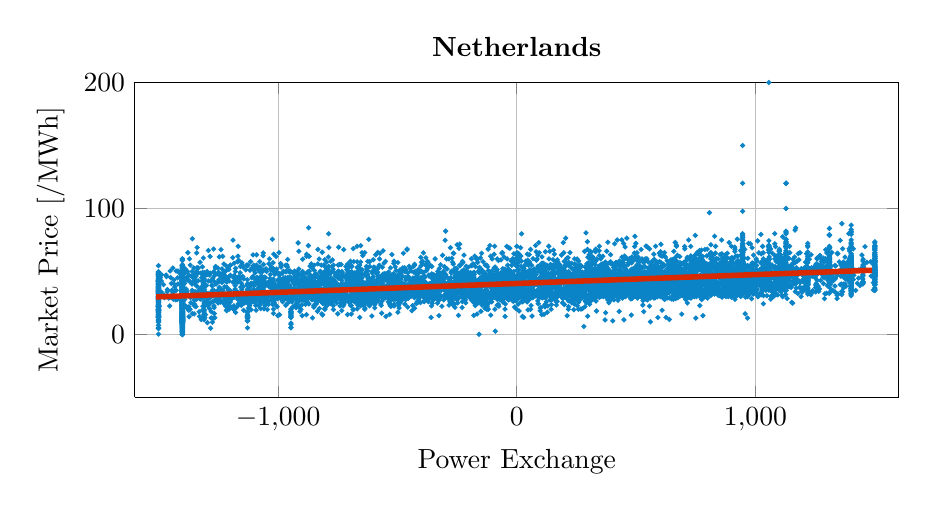
\begin{tikzpicture}

\begin{axis}[%
width=\fwidth,
height=\fheight,
at={(0\fwidth,0\fheight)},
scale only axis,
clip mode=individual,
separate axis lines,
every outer x axis line/.append style={black},
every x tick label/.append style={font=\color{black}},
xmin=-1600,
xmax=1600,
xlabel={Power Exchange},
xmajorgrids,
every outer y axis line/.append style={black},
every y tick label/.append style={font=\color{black}},
ymin=-50,
ymax=200,
ylabel={Market Price [\euro/MWh]},
xtick={-1000,0,1000},
ymajorgrids,
title style={font=\bfseries},
title={Netherlands}
]
\addplot [color=mycolor1,line width=1.0pt,mark size=0.3pt,only marks,mark=*,mark options={solid},forget plot]
  table[row sep=crcr]{%
-1401	15.15\\
-1401	12.96\\
-1401	12.09\\
-1401	11.7\\
-1401	11.66\\
-1401	11.35\\
-1401	9.85\\
-1401	9.54\\
-1401	9.49\\
-1401	11.64\\
-1401	11.94\\
-1401	13.15\\
-1401	15.24\\
-1401	13.69\\
-1401	12.43\\
-1401	9.92\\
-1401	12.12\\
-1401	15.24\\
-1401	15.73\\
-1401	17.73\\
-1401	15.63\\
-1401	13.93\\
-1401	15.1\\
-1401	12.95\\
-1401	9.62\\
-1401	7.64\\
-1283	4.96\\
-1401	0.06\\
-1401	1.05\\
-1401	7.08\\
-1401	12.5\\
-1401	21.31\\
-1401	30.44\\
-1401	35.48\\
-1401	33.06\\
-1401	33.78\\
-1401	37.97\\
-1401	37.42\\
-1401	36.24\\
-1401	32.18\\
-1401	33.56\\
-1401	52.94\\
-1292	66.7\\
-1147	53.53\\
-1401	39.54\\
-1401	35.9\\
-1016	35.47\\
-1308	30.64\\
-1351	27.4\\
-1401	25.23\\
-1401	15.63\\
-1401	8.74\\
-1401	11.28\\
-1401	12.34\\
-1401	26.02\\
-1401	31.66\\
-1401	31.96\\
-1401	31.94\\
-1401	30.96\\
-1401	31.45\\
-1401	39.05\\
-1401	30.99\\
-1401	30.46\\
-1401	30.43\\
-1401	31.12\\
-1401	36.98\\
-1401	34.97\\
-1401	42.18\\
-1401	30.39\\
-1401	26.32\\
-1105	31.82\\
-728	32.22\\
-1401	11.94\\
-1401	10.5\\
-1401	7.93\\
-1401	5.23\\
-1401	4.86\\
-1401	8.96\\
-1401	8.72\\
-1401	9.91\\
-1401	11.5\\
-1401	12.76\\
-1401	13.36\\
-1401	14.03\\
-1401	15.64\\
-1401	14.24\\
-1401	14.48\\
-1401	30\\
-1401	12.86\\
-1401	16.79\\
-1401	21.08\\
-1401	18.1\\
-1401	16.14\\
-1401	13.84\\
-1401	14.89\\
-1401	17.34\\
-1401	15.46\\
-1401	14.69\\
-1401	13.33\\
-1501	10.96\\
-1501	9.83\\
-1501	11.66\\
-1401	11\\
-1401	11.38\\
-1401	13.77\\
-1401	27.42\\
-1401	30.9\\
-1401	32.45\\
-1401	32.07\\
-1401	29.91\\
-1401	28.41\\
-1401	16.89\\
-1401	15.39\\
-1401	46.14\\
-1401	40.13\\
-1401	38.49\\
-1401	34.67\\
-1401	29.4\\
-1401	28.81\\
-1401	22.08\\
-1401	13.84\\
-1401	11.89\\
-1401	9.85\\
-1401	5.09\\
-1401	3.79\\
-1401	8.24\\
-1401	17.29\\
-1284	48.6\\
-1401	46.6\\
-1401	40\\
-1270	67.8\\
-1239	67.3\\
-1401	46.08\\
-1401	46.08\\
-1401	34.5\\
-1401	46.08\\
-1388	48.99\\
-872	84.71\\
-1401	54.57\\
-1401	50.7\\
-1401	41.75\\
-1401	28.34\\
-1401	38.52\\
-1348	33.69\\
-1401	9.26\\
-1401	9.98\\
-1401	3.88\\
-1401	0.07\\
-1401	2.05\\
-1401	6.52\\
-1401	26.07\\
-1401	34.99\\
-1401	49.42\\
-1401	52\\
-1401	52\\
-1401	54.36\\
-1334	52.78\\
-1401	49.99\\
-1401	45.93\\
-1401	43\\
-1401	46\\
-1401	54.44\\
-1285	61.93\\
-989	56.29\\
-1401	40.02\\
-1401	31.58\\
-1314	36.08\\
-1358	33.51\\
-1401	22.01\\
-1401	14.61\\
-1401	12.67\\
-1401	11.34\\
-1401	9.99\\
-1401	22.41\\
-1113	30.31\\
-259	46.42\\
-624	57.96\\
-616	57.82\\
-370	53.7\\
-574	54.51\\
-515	56.46\\
-866	54.3\\
-1024	51.11\\
-1358	47\\
-1235	52.06\\
-1167	70.01\\
-996	65\\
-1008	61.89\\
-1401	48.39\\
-1401	38.97\\
-1401	39.86\\
-1401	38.79\\
-1401	27.18\\
-1401	26.5\\
-1401	24.83\\
-1401	18.34\\
-1401	12.96\\
-1401	25.04\\
-601	34.65\\
-179	48\\
-1021	56.97\\
-1401	48.54\\
-1401	46.99\\
-1401	47.38\\
-1401	48.92\\
-1401	46.65\\
-1401	41.82\\
-1401	37.84\\
-1401	43.83\\
-1401	52.66\\
-1232	62.06\\
-897	59.78\\
-1295	47.89\\
-1401	40.66\\
-1088	45.35\\
-1093	44.29\\
-984	42.64\\
-654	38\\
-1158	32.2\\
-1401	16.27\\
-1401	15.49\\
-1093	33.77\\
-794	46.7\\
-311	62.87\\
-960	59.51\\
-1246	61.62\\
-1371	59.99\\
-1168	58.32\\
-1077	57.73\\
-1262	53.76\\
-1401	50.84\\
-1401	46.87\\
-1317	53.65\\
-1189	74.86\\
-913	66.02\\
-789	61.5\\
-1327	57.3\\
-1401	46.82\\
-306	50\\
-254	47.33\\
-166	40.36\\
-748	28.17\\
174	35.03\\
-605	28.26\\
-1268	26.76\\
-857	28.27\\
-40	34.12\\
-396	38.34\\
-994	43.65\\
-1157	45\\
-1401	46.36\\
-1401	46.34\\
-1077	49.72\\
-1401	41.89\\
-1401	37.94\\
-1401	38.34\\
-1401	40.28\\
-1401	51.79\\
-1401	59.12\\
-1401	58.65\\
-1401	50.94\\
-1401	44.8\\
-858	52.81\\
-691	48.69\\
-1129	43.47\\
-798	40\\
-1401	25.86\\
-1401	16.97\\
-1401	14.51\\
-1401	16.47\\
-1401	16.18\\
-1401	23.1\\
-1401	31.5\\
-1232	44.33\\
-1401	25.75\\
-1401	23.98\\
-1401	29.73\\
-1401	24.67\\
-1401	25.7\\
-1401	27.07\\
-1401	31.11\\
-1401	39.66\\
-1401	41.96\\
-1359	46.09\\
-1401	37.35\\
-1501	32.85\\
-799	37.62\\
-344	32.17\\
-981	26\\
-1424	27.86\\
-1501	27.6\\
-1501	13.45\\
-1501	14.24\\
-1215	26.71\\
-403	33.11\\
292	50.84\\
-464	51.45\\
-664	53.89\\
-573	64.36\\
-582	65.14\\
-709	55.89\\
-809	55\\
-849	54.94\\
-768	54.97\\
-374	57.93\\
-833	67.48\\
-475	64.41\\
-152	60.71\\
-255	51.62\\
-1228	44.67\\
-869	43.21\\
-523	43.21\\
-432	31.14\\
-865	29.65\\
-633	29.56\\
-1501	24.17\\
-1501	19.72\\
-796	30.34\\
-179	36.98\\
352	60.09\\
309	65.94\\
377	66.06\\
154	66.95\\
58	67.51\\
135	60.02\\
126	55.01\\
187	52.54\\
-34	51.86\\
-266	55.88\\
79	70.68\\
704	68\\
892	53.7\\
982	54.94\\
-713	45.14\\
-315	44.94\\
-275	39.99\\
-567	33.03\\
-617	30.66\\
-883	29.92\\
-1393	29.63\\
-1393	29.54\\
-799	30.65\\
119	39.94\\
-428	55.67\\
-645	62.65\\
-780	58.07\\
-736	55.47\\
-691	53.9\\
-451	54.16\\
-402	54.35\\
-505	50.75\\
-950	50.51\\
-1209	52.1\\
-1184	56.49\\
-221	62.96\\
314	61.29\\
-524	47\\
-1401	38.6\\
-967	39.46\\
-509	35.75\\
-985	30.06\\
-1320	28.92\\
-1401	25.6\\
-1401	21.42\\
-1401	18.42\\
-1111	28.66\\
-448	33.35\\
-106	50.09\\
-806	48.34\\
-1032	51.57\\
-1101	50.84\\
-1050	52.2\\
-1206	51.52\\
-1152	55\\
-1200	54.94\\
-1029	53.62\\
-963	55\\
-788	79.94\\
-1401	55.55\\
-1368	55\\
-1401	46.02\\
-1401	35.23\\
-1400	37.69\\
-776	38\\
-1194	29.53\\
-1401	28.17\\
-1401	19.58\\
-1401	11.23\\
-1401	11.18\\
-1401	20.74\\
-648	34.03\\
-917	48.97\\
-1297	49.96\\
-1501	47.71\\
-1501	47.91\\
-1501	47.96\\
-1501	48.68\\
-1501	46.17\\
-1501	42.32\\
-1488	47.44\\
-1335	48.87\\
-1339	68.99\\
-1441	52.75\\
-1005	49.43\\
-1501	43.74\\
-1501	33.33\\
-1243	34.45\\
-767	35.9\\
-967	30.5\\
-1310	29.79\\
-1501	28.58\\
-1501	26.79\\
-1501	18.63\\
-1501	22.25\\
-1501	22\\
-1469	30.25\\
-1496	33.34\\
-1501	39.96\\
-1501	35.17\\
-1501	32.44\\
-1401	31.28\\
-1401	30.89\\
-1401	30.68\\
-1401	30.88\\
-1401	33.17\\
-1401	54.53\\
-1401	45.05\\
-1401	39.72\\
-1401	30.21\\
-1401	28.63\\
-1401	30.4\\
-641	38.63\\
-575	36.1\\
-1018	30.14\\
-1401	26.15\\
-1401	9.48\\
-1401	12.8\\
-1401	16.41\\
-1401	12.18\\
-1401	15.76\\
-1401	29.99\\
-1156	37.57\\
-1401	44.38\\
-1401	46.47\\
-1379	49.96\\
-1401	44.12\\
-1401	35.64\\
-1401	27.42\\
-1401	29.67\\
-1313	60.71\\
-1401	60\\
-1401	46.54\\
-1401	42.51\\
-1401	40.02\\
-1401	41.86\\
-951	38\\
-549	34.75\\
-1185	29.46\\
-1259	29.21\\
-1401	14.99\\
-1367	29.33\\
-1401	25.5\\
-182	45.93\\
410	71.97\\
669	70.92\\
597	64.5\\
939	62.93\\
765	64.44\\
777	59.61\\
648	58.04\\
431	54.16\\
201	49.7\\
86	52.53\\
197	64.91\\
829	77.99\\
1024	63.97\\
346	62.7\\
-1427	50.4\\
-514	58.17\\
-749	49.38\\
-435	44.79\\
-480	34.35\\
-902	30.65\\
-991	30.3\\
-1041	30.65\\
-357	33.68\\
139	45.86\\
502	59.91\\
187	62.98\\
68	60.19\\
52	63.32\\
81	65.65\\
88	62.91\\
-53	61.46\\
203	57.41\\
-119	50.81\\
-212	54.09\\
-17	60.23\\
773	60.57\\
992	62.97\\
894	52.97\\
6	48.03\\
55	51.45\\
-297	47.44\\
-207	45.67\\
-10	43.09\\
-243	34.97\\
-514	31.02\\
-1014	31.14\\
-102	35.41\\
576	48.5\\
788	67.49\\
345	66.49\\
603	65.66\\
454	60.88\\
601	62.79\\
509	61.44\\
485	59.37\\
659	58.96\\
742	54.76\\
497	61.62\\
604	71.58\\
1081	80.06\\
1345	64.04\\
1501	62\\
1061	53.5\\
1501	61.58\\
1453	53.5\\
-248	41.81\\
114	41.5\\
-32	39.22\\
-911	31.32\\
-1050	31.17\\
-156	34.03\\
340	43.13\\
1258	60.59\\
1305	65.1\\
1320	65.05\\
1187	64.92\\
1087	62.17\\
951	60.92\\
869	60.91\\
617	54.77\\
264	49.69\\
75	48.08\\
155	55.17\\
810	63.96\\
1102	57.53\\
-122	53.78\\
-1401	45.45\\
-803	53.8\\
-729	46.91\\
-650	35.05\\
-669	32.29\\
-1363	30.34\\
-1401	29.99\\
-1401	30.53\\
-1075	32.17\\
110	43.42\\
1058	61.6\\
617	62.5\\
393	63.3\\
318	61.59\\
303	63.28\\
319	60.39\\
152	59.33\\
644	58.97\\
450	53.19\\
253	53.03\\
-62	64.41\\
504	64.94\\
574	63.71\\
207	54.64\\
-932	50.15\\
-1287	47.09\\
-938	49\\
-1433	37.68\\
-1047	32.05\\
-1497	31.1\\
-1501	30.32\\
-1501	29.83\\
-1501	29.04\\
-1401	30.9\\
-1401	31.58\\
-1401	39.27\\
-1401	42.04\\
-1401	43.63\\
-1401	44.11\\
-1401	45.82\\
-1401	37.68\\
-1401	32.69\\
-1401	32.69\\
-1401	33.57\\
-1401	38.13\\
-1401	48.04\\
-1401	43.14\\
-1401	32.57\\
-1401	30.05\\
-1401	32.86\\
-606	38.23\\
-1004	22.11\\
-1374	19.14\\
-1401	14.85\\
-1401	13.14\\
-1401	13.22\\
-1401	12.73\\
-1401	9.53\\
-1401	14.05\\
-1401	14.04\\
-1501	22.19\\
-1501	22.69\\
-1501	22.85\\
-1501	23.42\\
-1501	19.08\\
-1501	15.23\\
-1401	12.89\\
-1401	8.26\\
-1401	17.66\\
-1401	22.42\\
-1401	26.7\\
-1401	31.96\\
-1401	23.75\\
-1401	28.24\\
-1401	20.29\\
-1401	12.63\\
-1401	11.74\\
-1401	12.81\\
-1401	7.1\\
-1401	8.77\\
-1401	13.09\\
-1172	30.14\\
-649	47.43\\
-1069	51.07\\
-1178	52.47\\
-1075	53.47\\
-1110	52.73\\
-834	56.05\\
-1074	50.71\\
-1006	51.92\\
-913	51.92\\
-712	51.47\\
-1061	55.53\\
20	79.92\\
8	64.25\\
-671	47.25\\
-1100	38.71\\
-265	40.2\\
60	38.51\\
-452	36.41\\
-640	32.92\\
-666	30.28\\
-1046	29.57\\
-1190	30.16\\
-548	31.21\\
174	41.47\\
668	55.05\\
-1	56.58\\
-239	54.52\\
-292	52\\
-259	52.44\\
-162	49.94\\
-348	47.44\\
-356	46.5\\
-548	48\\
-631	49.77\\
-669	57.75\\
-93	70\\
-109	62.09\\
-226	56.94\\
-1301	47.4\\
-204	53.42\\
209	48.28\\
-313	38.65\\
-442	30.54\\
-667	29.63\\
-1193	28.98\\
-832	29.55\\
-345	31.08\\
754	37.1\\
1401	55.38\\
1375	52.95\\
1401	52.9\\
938	57.44\\
987	56.78\\
905	53.55\\
1258	54\\
1200	50.01\\
881	47.44\\
752	47.02\\
1164	61.52\\
1401	83.27\\
1401	72.99\\
1336	54.43\\
1117	49.5\\
1401	54.11\\
1401	52.05\\
840	37.75\\
613	34.94\\
625	34.29\\
-102	29.92\\
-318	30.32\\
429	34.43\\
790	45.2\\
979	53.07\\
1401	54.73\\
1299	64.78\\
1115	59.99\\
1179	64.16\\
1088	59.72\\
865	54.48\\
792	51.89\\
1018	51.5\\
817	51.56\\
754	55.12\\
1410	67.98\\
1451	59.67\\
1272	50.5\\
371	45.81\\
661	46.52\\
1342	47.1\\
770	42.96\\
932	42.5\\
827	36.54\\
663	33.06\\
481	31.95\\
852	40.03\\
508	46.9\\
1143	69.94\\
1081	71.95\\
448	72.19\\
284	65.88\\
215	60.93\\
176	52.93\\
158	48.14\\
-546	45\\
-565	44.1\\
-901	44.23\\
-470	52.92\\
683	61.76\\
691	56.35\\
-141	49.08\\
-478	40\\
323	41.99\\
739	39.17\\
-428	31.04\\
-1066	28.94\\
-1401	26.63\\
-1401	20.87\\
-1401	20.18\\
-1401	20.71\\
-1401	26.82\\
-1401	28.7\\
-1401	37.27\\
-1401	42.65\\
-1401	43.28\\
-1401	44.55\\
-1310	48.59\\
-1310	40.24\\
-1310	32.87\\
-1401	32.8\\
-1401	33.28\\
-1401	43.56\\
-1179	50.02\\
-1382	44.94\\
-1401	41.24\\
-1238	35.81\\
-844	35.01\\
-328	35.96\\
393	41.62\\
-32	31.96\\
-735	25.8\\
-1316	19.38\\
-1265	13.18\\
-1373	14.07\\
-1359	16.54\\
-1501	18.85\\
-1501	22.07\\
-1188	30.83\\
-1214	31.96\\
-1401	31.82\\
-1404	34.15\\
-1501	32.14\\
-1501	30.8\\
-1501	31.03\\
-1501	32.95\\
-1501	36.15\\
-1501	48.68\\
-1501	54.57\\
-1261	53.78\\
-1165	45.76\\
-488	49.81\\
290	48.84\\
-227	44.37\\
-180	37.8\\
-263	36\\
-681	31.56\\
-541	31.52\\
281	36.19\\
739	54.1\\
979	71.89\\
890	72.94\\
521	67.5\\
218	57.18\\
262	54.63\\
378	52.9\\
416	51.96\\
261	46.82\\
194	47.14\\
129	46.76\\
107	54.09\\
798	67.8\\
813	59.96\\
-227	57.98\\
-1341	48.72\\
-628	52.2\\
-59	52.27\\
-399	44.42\\
333	44.96\\
92	40.9\\
-514	30.63\\
-461	30\\
-254	32.38\\
479	47.13\\
209	60.3\\
-24	58.49\\
-356	53.88\\
-592	51.99\\
-478	52.83\\
-187	54.68\\
-411	51.68\\
-516	48.05\\
-544	47.59\\
-647	48.03\\
-668	53.05\\
-12	63.99\\
47	55.73\\
-356	48\\
-1501	41.26\\
-996	44.08\\
-541	42.46\\
-464	30.53\\
-614	29.98\\
-711	28.99\\
-1401	25.71\\
-1401	18.11\\
-936	28.08\\
-579	33.51\\
-1358	45.16\\
-1341	49.94\\
-1252	52.61\\
-1164	58.57\\
-1216	54.16\\
-1255	48.08\\
-1087	52.2\\
-1020	50.09\\
-1401	43.92\\
-1401	42.55\\
-1344	49.69\\
-725	67.38\\
-600	53.32\\
-1401	36.79\\
416	57.1\\
990	52\\
1036	45\\
1401	42.28\\
1314	39.94\\
808	34.79\\
-135	28.27\\
-115	28.67\\
896	32.2\\
1401	44\\
1401	55.87\\
1401	56.7\\
1401	58.84\\
1401	61.77\\
1401	60.43\\
1401	57.28\\
1401	55.91\\
1001	55.29\\
927	49.94\\
415	47.89\\
245	55.89\\
658	66.01\\
1401	60.02\\
492	48.05\\
-763	37.12\\
-475	33.71\\
-67	39.61\\
-1401	23.64\\
-1401	19.51\\
-1401	14.66\\
-1401	12.18\\
-1401	8.54\\
-1401	15.42\\
-1401	30.68\\
-1014	47.79\\
-1206	45.71\\
-1401	47.63\\
-1401	47.94\\
-1401	51.34\\
-1401	48.37\\
-1401	42.94\\
-1401	36.86\\
-1401	32.31\\
-1401	31.3\\
-1401	36.16\\
-1401	59.92\\
-1401	54.71\\
-1401	43.31\\
-1401	30.49\\
-1401	38.37\\
-1401	40.84\\
-1401	28\\
-1401	26.43\\
-1401	25.9\\
-1401	24.93\\
-1401	10.52\\
-1401	16.2\\
-1401	24.04\\
-1401	27.13\\
-1401	29.51\\
-1401	29.48\\
-1401	28.07\\
-1401	26.76\\
-1401	28.03\\
-1401	25.5\\
-1401	25.96\\
-1401	28.81\\
-1401	28.03\\
-1401	31.17\\
-1401	42.58\\
-1401	33.88\\
-1401	27.57\\
-1401	24.29\\
-1401	27.55\\
-1401	23.6\\
-1401	14.23\\
-1401	13.02\\
-1401	12.87\\
-1322	11.77\\
-1275	9.72\\
-1296	9.36\\
-1401	10.63\\
-1401	10.54\\
-1401	11.04\\
-1401	19.16\\
-1401	17.7\\
-1401	17.29\\
-1401	14.68\\
-1401	13.16\\
-1401	10.5\\
-1401	8.97\\
-1401	12.42\\
-1401	14.69\\
-1401	35.79\\
-1401	36.81\\
-1401	31.23\\
-1401	27.97\\
-1229	30.04\\
-1401	25.31\\
33	36.13\\
-297	33.87\\
-1135	27.22\\
-1401	23.86\\
-1154	23.08\\
-15	33.18\\
1139	45.43\\
1401	59.42\\
1401	60.99\\
1401	58.79\\
1393	60.02\\
1151	54.96\\
1255	56.12\\
1166	56.82\\
1260	55.63\\
1084	51.47\\
743	47.44\\
923	54.94\\
1401	79.49\\
1401	54.32\\
1401	50.06\\
359	46.57\\
664	47.59\\
245	42.83\\
-557	30.75\\
-218	32.07\\
-264	29.45\\
-904	28.27\\
-1256	28.05\\
-626	30.72\\
119	41.12\\
-303	53.8\\
-319	55.34\\
-556	56.62\\
-788	54.1\\
-585	51.74\\
-443	50.38\\
-415	49.25\\
-863	42.49\\
-1046	39.56\\
-775	41\\
-49	51.9\\
46	58.97\\
296	67.49\\
-39	50\\
-760	46.48\\
275	49.48\\
225	44.09\\
326	45\\
137	41.94\\
32	37.84\\
-264	28.43\\
-300	29.36\\
104	36.72\\
973	45.54\\
946	59.3\\
331	65.77\\
-29	68.42\\
-381	60.87\\
-184	55.9\\
-142	50.33\\
-254	49.42\\
-571	45.92\\
-781	43.34\\
-1046	40.93\\
-571	44.99\\
82	58.94\\
428	54.37\\
-375	52.03\\
-1374	42.78\\
-145	46.13\\
194	44.03\\
-83	42.97\\
-179	34.54\\
-586	32.23\\
-1401	18.33\\
-1401	12.47\\
-1401	26.67\\
-537	42.44\\
-182	55.88\\
-91	53.54\\
-141	57.79\\
-374	56.72\\
-550	57.98\\
-362	55\\
-529	52.89\\
-593	52.35\\
-960	45.25\\
-1376	42.91\\
-893	48.66\\
-34	68.92\\
-19	58.69\\
-1353	52.81\\
-1401	42\\
-1045	40.63\\
-332	38.04\\
-876	33\\
-798	32.72\\
-777	29.33\\
-1401	24.42\\
-1401	25.63\\
-1401	29.44\\
-94	46.4\\
-402	61.12\\
-391	64.8\\
-746	69.25\\
-1168	62.12\\
-1132	55\\
-1096	52.08\\
-1373	47.1\\
-1401	44.22\\
-1401	36.2\\
-1401	40\\
-1401	46.18\\
-961	53.48\\
-880	48.73\\
-1401	36.97\\
-1401	30.39\\
-1401	30.61\\
-1246	42.44\\
-1401	27.73\\
-1401	17.99\\
-1401	12.38\\
-1401	10.36\\
-1401	10.11\\
-1401	10.33\\
-1401	11.36\\
-1401	13.34\\
-1401	18.26\\
-1401	22.66\\
-1401	23.11\\
-1401	23.08\\
-1401	23.76\\
-1401	22.48\\
-1401	21.11\\
-1401	19.33\\
-1401	20.46\\
-1401	27.73\\
-1401	39.29\\
-1401	44.85\\
-1401	28.93\\
-1401	29.36\\
-1401	41.5\\
-1075	41.56\\
-1401	25.49\\
-1401	14.46\\
-1401	12.35\\
-1401	9.06\\
-1401	5.3\\
-1401	8.08\\
-1401	11.12\\
-1401	9.53\\
-1401	10.73\\
-1401	13.37\\
-1401	16.81\\
-1401	17.86\\
-1401	18.23\\
-1401	13.15\\
-1401	11.38\\
-1401	10.48\\
-1401	12.22\\
-1401	15.26\\
-1401	40.15\\
-1401	47.98\\
-1401	46.83\\
-1401	34.73\\
-1401	39.08\\
-1401	31.53\\
-1401	31.59\\
-1401	25.69\\
-1401	23.33\\
-1401	17.52\\
-1401	19.63\\
-1401	26.47\\
-689	43.79\\
-77	58.75\\
-596	53.31\\
-1158	54\\
-1227	49.32\\
-930	50\\
-1211	44.22\\
-1501	42.07\\
-1501	34.96\\
-1501	37.25\\
-1501	40.33\\
-1501	43.03\\
-298	82.04\\
-239	71.74\\
230	56.51\\
-660	47.19\\
98	49.94\\
-530	43.43\\
-823	31.95\\
-741	31.66\\
-736	30.09\\
-802	28.86\\
-859	29.2\\
-737	31.3\\
-92	42.03\\
294	56.19\\
514	54.9\\
558	53.79\\
676	51.9\\
755	50.74\\
847	51.42\\
654	48.48\\
16	43.27\\
-107	43.44\\
-183	45.72\\
-173	53.91\\
296	73.68\\
525	59.98\\
-181	45.94\\
-1501	39.68\\
-975	41.9\\
-781	36.47\\
-864	32.16\\
-658	29.65\\
-1002	28.46\\
-1402	27.67\\
-1501	28.51\\
-997	29.34\\
-256	38.19\\
-76	47.45\\
-488	49.44\\
-793	52.21\\
-716	53.93\\
-616	53.96\\
-483	50.76\\
-590	49.48\\
-583	49.37\\
-586	47.95\\
-737	44.71\\
-356	47.44\\
582	70\\
651	59.54\\
454	54.27\\
-847	47.02\\
-1144	44.18\\
-514	44.96\\
-574	31.28\\
-408	29.47\\
-1066	28.87\\
-1160	27.75\\
-1501	25.59\\
-1074	27.85\\
-222	34.51\\
-479	46.28\\
-239	48.34\\
-553	48.28\\
-1172	44.93\\
-864	46.95\\
-685	47.58\\
-1349	44.94\\
-1401	40.02\\
-1401	34.96\\
-1401	32.45\\
-1401	41.78\\
-1090	55\\
-1073	52.17\\
-1238	47.44\\
-1401	39.95\\
-1401	41.78\\
-1189	41.49\\
-1389	32.91\\
-1401	22.15\\
-1401	20.84\\
-1401	19.42\\
-1401	21.02\\
-1401	26.64\\
-1401	35.83\\
-1344	46.31\\
-1267	49.03\\
-1401	52.95\\
-1401	50.07\\
-1401	48.45\\
-1401	42.88\\
-1401	37.61\\
-1401	32.16\\
-1401	32.1\\
-1401	31.68\\
-1401	42.9\\
-803	49.44\\
-424	49.96\\
-1317	49.08\\
-1401	40.71\\
-837	40.93\\
-300	41\\
-71	35.11\\
-302	29.96\\
-835	26.09\\
-1401	21.02\\
-1401	18.67\\
-1401	21.15\\
-939	27.93\\
-1045	29.38\\
-1401	32.92\\
-1401	37.43\\
-1401	37.35\\
-1401	36.86\\
-1401	38.85\\
-1401	35.47\\
-1401	29.59\\
-1401	31.99\\
-1401	31.33\\
-1401	37.71\\
-1401	50.91\\
-1339	53.1\\
-1401	44.22\\
-1501	36.72\\
-1115	40.34\\
-653	36.96\\
-1401	26.11\\
-1401	21.63\\
-1401	22.07\\
-1401	19.48\\
-1401	16.28\\
-1401	19.86\\
-1304	15.73\\
-1401	15.73\\
-1401	17.1\\
-1401	16.63\\
-1401	17.46\\
-1401	16.77\\
-1401	14.68\\
-1401	12.98\\
-1401	11.26\\
-1401	7.45\\
-1401	10.84\\
-1401	11.28\\
-1401	24.31\\
-1401	35.49\\
-1401	27.81\\
-1401	23.11\\
-1401	27.1\\
-1241	25.71\\
-1401	14.5\\
-1401	15.09\\
-1401	17.22\\
-1401	13.68\\
-1401	14\\
-1401	18.12\\
-778	35.66\\
-920	46.95\\
-949	50\\
-1401	46.65\\
-1401	45.98\\
-1401	41.79\\
-1401	40.46\\
-1401	39.32\\
-1401	35.99\\
-1401	31.07\\
-1401	32.97\\
-1401	46.16\\
-1378	64.95\\
-1341	64.73\\
-1401	48.99\\
-1401	35.43\\
-1080	37.44\\
-646	33.87\\
-589	26.22\\
-1040	23.87\\
-1185	22.77\\
-1501	20.29\\
-1501	18.97\\
-719	25.94\\
-79	36.97\\
49	46.95\\
-691	46.66\\
-1501	46.12\\
-1501	44.59\\
-1501	44\\
-1421	44.94\\
-1501	40.49\\
-1501	36.09\\
-1501	35.3\\
-1501	33.71\\
-1501	42.61\\
-916	72.68\\
-1063	62.52\\
-1184	46.87\\
-1501	39.88\\
-733	42.89\\
-319	39.59\\
-610	36.05\\
-730	30\\
-904	27.29\\
-784	26.91\\
-731	27.86\\
-727	28.48\\
-413	39.22\\
-260	45.05\\
-777	49.24\\
-1135	51.3\\
-1452	50.42\\
-1269	50\\
-1265	46.91\\
-1242	46.42\\
-1320	44.96\\
-1164	43.35\\
-1401	41.81\\
-972	43.99\\
-250	71.19\\
195	72.95\\
44	49.85\\
-304	45.59\\
-410	42.44\\
-163	40.05\\
-348	33.99\\
-327	32.03\\
-356	30.28\\
-387	29.61\\
-511	29.48\\
-133	32.18\\
-615	41.54\\
-563	53.34\\
-869	50.1\\
-1469	47.1\\
-1501	48.14\\
-1148	46\\
-957	44.24\\
-920	44.81\\
-987	43.22\\
-1249	41.94\\
-1392	40.62\\
-770	51.76\\
-637	64.96\\
-1115	57.83\\
-1324	48.66\\
-1249	43.21\\
-961	41.45\\
-934	40.16\\
-759	36.25\\
-574	34.94\\
-727	30.19\\
-819	28.03\\
-718	28.54\\
-750	29.94\\
-832	39.6\\
-908	47.45\\
-1501	49.45\\
-1501	49.77\\
-1501	49.12\\
-1501	47.42\\
-1501	46.72\\
-1501	44.7\\
-1501	42.31\\
-1501	41.92\\
-1501	42.98\\
-1501	47.3\\
-1062	64.68\\
-828	59.92\\
-1305	47.28\\
-1401	39.75\\
-773	42.95\\
-423	42\\
-700	40.61\\
-585	35.72\\
-507	33.79\\
-661	30.22\\
-869	29.28\\
-873	29.33\\
-1148	28.98\\
-1347	33.71\\
-1480	39.51\\
-1315	47.4\\
-1420	50.34\\
-1410	48.18\\
-1230	47.97\\
-1437	43.25\\
-1501	38.63\\
-1501	36.46\\
-1501	33.77\\
-1347	41.27\\
-591	63.21\\
-300	74.76\\
-950	45.93\\
-822	42.66\\
190	48.38\\
25	44.97\\
244	44.94\\
-137	39.4\\
-237	32.28\\
-379	29.31\\
-494	27.57\\
-507	27.86\\
-774	27.33\\
-1149	27.04\\
-773	27.49\\
-1106	32.39\\
-1079	33.69\\
-1067	33.67\\
-1064	34.38\\
-1501	27.45\\
-1501	23.55\\
-1401	24.59\\
-1401	25.42\\
-1401	28.22\\
-1401	33.96\\
-1164	42.62\\
-1400	39.44\\
-1208	31.89\\
-424	36.16\\
184	32.59\\
-564	26.52\\
-636	25.11\\
-1014	24.08\\
-1384	22.14\\
-1355	24.03\\
-580	27.01\\
411	43.93\\
-23	49.94\\
-222	51.33\\
-509	53.68\\
-648	51.43\\
-498	57.13\\
-625	47.83\\
-584	49.41\\
-625	46.48\\
-1128	38.95\\
-891	40.98\\
-710	44.96\\
92	72.91\\
290	80.69\\
-36	47.81\\
-251	43.99\\
222	45.3\\
-35	43.34\\
765	45.03\\
454	39.19\\
165	33.29\\
-242	28.99\\
-279	29.68\\
47	33.28\\
880	47.18\\
434	53.9\\
664	57.9\\
666	57.32\\
735	51.02\\
815	51.98\\
1128	52.3\\
987	50\\
876	48.59\\
601	46.51\\
389	45.92\\
288	45.87\\
924	75.64\\
1023	79.38\\
684	54.77\\
119	50.68\\
872	49.01\\
1128	50.54\\
381	40.21\\
540	39.94\\
809	42.1\\
530	34.72\\
333	33.37\\
508	41.28\\
420	47.32\\
-176	62.16\\
-120	67.76\\
-685	68.08\\
-704	53.01\\
-845	44.96\\
-958	43.85\\
-739	44.19\\
-1501	40.21\\
-1501	38.02\\
-1501	38.08\\
-738	46.54\\
-394	58.03\\
-242	68.37\\
-821	49.04\\
-1335	42.58\\
-553	45.99\\
-305	44.1\\
-476	37.43\\
-528	36.72\\
-412	34.14\\
-654	28.81\\
-607	29.19\\
-402	33.98\\
-137	42.85\\
180	55.33\\
300	56.97\\
-395	56.22\\
-692	50\\
-652	48.58\\
-508	46.41\\
-807	44.92\\
-1447	40.51\\
-1501	34.11\\
-1501	37\\
-741	45\\
106	61.59\\
1084	69.75\\
366	53.9\\
-687	42.17\\
317	45.73\\
483	40.97\\
720	40.01\\
273	33.98\\
6	32.22\\
-256	28.9\\
-176	29.1\\
219	32.06\\
-52	40.9\\
-414	48.26\\
-664	53.76\\
-881	62\\
-1310	49.17\\
-1215	45.36\\
-1273	44.82\\
-1501	37.93\\
-1501	35.64\\
-1501	31.97\\
-1501	31.94\\
-1501	39.36\\
-1225	47.09\\
-1249	49.26\\
-1467	45.95\\
-1501	41.92\\
-825	44.28\\
-538	43.68\\
-842	39.97\\
-1016	33.31\\
-1091	30.44\\
-1043	25.71\\
-959	24.96\\
-941	25.82\\
-1056	26.92\\
-1225	29.6\\
-1401	31.96\\
-1401	31.51\\
-1401	28.19\\
-1401	26.17\\
-1401	24.42\\
-1401	20.02\\
-1401	15.91\\
-1401	12.03\\
-1401	16.02\\
-1401	22.55\\
-1401	35.58\\
-1401	42.77\\
-1401	30.03\\
-1401	25.14\\
-1016	25.47\\
-595	23.65\\
-994	15.67\\
-1401	13.75\\
-1401	12.1\\
-1401	11.4\\
-1401	10.35\\
-1401	11.4\\
-1401	11.49\\
-1401	11.4\\
-1401	11.55\\
-1401	12.05\\
-1401	11.54\\
-1401	12.11\\
-1401	12.26\\
-1401	10.29\\
-1401	6.2\\
-1401	1.75\\
-1401	1.87\\
-1401	9.83\\
-1401	22.41\\
-1401	41.73\\
-1401	34.86\\
-1401	28.07\\
-1367	30.09\\
-665	26.92\\
-871	24.26\\
-1293	22.62\\
-1350	22.73\\
-1401	22.76\\
-1401	22.11\\
-1076	25.57\\
-586	43.5\\
-993	48.28\\
-1312	48.12\\
-1401	44.76\\
-1401	40.9\\
-1401	37.42\\
-1401	36.46\\
-1401	35.85\\
-1401	33.8\\
-1401	30.13\\
-1401	30.19\\
-1401	36.36\\
-861	56.07\\
-620	75.46\\
-756	46.32\\
-1401	38.68\\
-1083	35.17\\
-716	30.93\\
-679	25.83\\
-598	25.9\\
-790	24.63\\
-1399	24.27\\
-1401	23.78\\
-1041	26.5\\
-740	35.08\\
-1346	42.55\\
-1401	44.58\\
-1401	40.03\\
-1401	40.2\\
-1401	36.07\\
-1401	31.88\\
-1401	30.65\\
-1401	28.18\\
-1401	28.72\\
-1401	30.91\\
-1401	36.26\\
-1360	49.94\\
-1401	54.1\\
-1401	42.56\\
-1401	34.04\\
-1024	40.03\\
-993	32.99\\
-1217	28.87\\
-1025	28.04\\
-1057	26.65\\
-1365	25.15\\
-1200	25.69\\
-1045	28.09\\
-1401	35.8\\
-1401	44.54\\
-1401	43.73\\
-1401	41.27\\
-1401	32.59\\
-1401	33.67\\
-1401	30\\
-1401	28.78\\
-1401	28.42\\
-1401	29.25\\
-1401	30.79\\
-1401	37.04\\
-1401	49\\
-1359	75.98\\
-1401	48.43\\
-1401	42.01\\
-1401	38.28\\
-1401	32.08\\
-1401	31.35\\
-1401	30.65\\
-1387	29.96\\
-1318	30\\
-1172	30.11\\
-1185	31.43\\
-1401	43.03\\
-988	53.46\\
-1401	49.84\\
-1401	41.27\\
-1401	34.74\\
-1401	29.77\\
-1401	30.58\\
-1401	28.42\\
-1401	28.78\\
-1401	30.95\\
-1401	35.54\\
-1401	30.84\\
-1263	52.76\\
-1024	75.55\\
-982	48.69\\
-1401	43.63\\
-1401	42.87\\
-1401	40.69\\
-1401	34.96\\
-1313	32.01\\
-1397	30.99\\
-1401	29.57\\
-1401	29.65\\
-1299	32.89\\
-1401	42.04\\
-805	49.94\\
-1401	47.93\\
-1401	42.94\\
-1401	41.26\\
-1401	38.83\\
-1401	37.01\\
-1401	34.91\\
-1401	30.96\\
-1401	29.53\\
-1401	30.91\\
-1401	37.91\\
-1151	45.07\\
-630	53.95\\
-1226	49.94\\
-1401	38.64\\
-1180	42.44\\
-1116	38.99\\
-874	28.64\\
-1216	18.86\\
-1401	21.1\\
-1401	11.3\\
-1401	7.58\\
-1401	11.81\\
-1401	13.36\\
-1401	14.02\\
-1401	22.83\\
-1401	20.01\\
-1401	16.52\\
-1401	15.8\\
-1401	21.57\\
-1401	15.2\\
-1401	12.55\\
-1401	11.78\\
-1401	11.26\\
-1401	18.81\\
-1399	44.94\\
-1401	48\\
-1401	25.54\\
-1401	23.29\\
-1401	20.33\\
-1401	19.29\\
-1401	15.89\\
-1401	14.23\\
-1401	13.29\\
-1401	11.77\\
-1401	11.11\\
-1401	10.12\\
-1401	11.23\\
-1401	10.91\\
-1401	11.44\\
-1401	10.77\\
-1401	12.34\\
-1401	13.02\\
-1401	13.95\\
-1401	11.07\\
-1401	9.33\\
-1401	3.07\\
-1401	5.41\\
-1401	9.43\\
-1401	22.78\\
-1389	52\\
-1401	49\\
-1401	21.31\\
-1401	20.51\\
-1401	28.62\\
-814	29.73\\
-783	26.33\\
-885	23.93\\
-1401	20.73\\
-1374	21.96\\
-918	26.41\\
-650	42\\
-848	50.81\\
-678	49\\
-1151	56.84\\
-772	59.16\\
-815	65.27\\
-1007	50\\
-824	50\\
-799	49.96\\
-706	49.08\\
-595	51.87\\
-459	67.78\\
-837	47.44\\
-669	69.94\\
-969	54.86\\
-1020	44\\
-976	45\\
-991	44.25\\
-580	31.57\\
-333	32.18\\
-648	29.99\\
-658	24.07\\
-332	24.89\\
-282	28.06\\
-201	40.44\\
-537	49.49\\
-978	50.12\\
-1018	63.77\\
-1125	55\\
-870	61.99\\
-697	58.13\\
-793	52.24\\
-895	45.13\\
-979	42\\
-1017	41.36\\
-822	42.44\\
-963	39.68\\
-227	46.28\\
-563	41.55\\
-1300	39\\
-973	32.73\\
-862	30.33\\
-1401	22.2\\
-1220	22.46\\
-1329	14.3\\
-1315	22.46\\
-1108	29.66\\
-1350	27.44\\
-711	42.36\\
-479	49.79\\
-1301	47.99\\
-1401	48\\
-1401	39.01\\
-1401	34.72\\
-1401	33.41\\
-1401	32.59\\
-1401	31.48\\
-1401	28.19\\
-1401	42.44\\
-1032	47.59\\
-1319	42.44\\
-1102	54.97\\
-1096	49\\
-1100	45\\
-939	44\\
-1056	41.93\\
-618	26.47\\
-489	26.72\\
-1126	24.54\\
-1401	17.18\\
-1331	18.05\\
-812	24.57\\
-96	37.54\\
-109	46.15\\
-1401	41.33\\
-1401	35.3\\
-1401	31.3\\
-1401	29.01\\
-1401	26.8\\
-1401	26.56\\
-1401	25.76\\
-1401	26.52\\
-1401	26.84\\
-1401	28.95\\
-1401	36.94\\
-1401	45.07\\
-1401	32\\
-1401	27.84\\
-1401	31.24\\
-983	30.47\\
-924	21.24\\
-1401	12.08\\
-1401	11.32\\
-1401	10.25\\
-1401	10.65\\
-1401	18.63\\
-1212	29.62\\
-1112	40\\
-1401	39.18\\
-1401	38.33\\
-1401	44.54\\
-880	63.62\\
-1169	57.66\\
-1227	55.89\\
-1383	45\\
-1361	39.96\\
-1348	39.94\\
-1401	38.93\\
-782	42.43\\
-658	55\\
-752	47.39\\
-465	43.08\\
-19	43.08\\
420	36.5\\
-245	33.94\\
-538	28.54\\
-513	24.08\\
-1501	19.07\\
-1501	13.66\\
-1501	17.92\\
-694	22.76\\
-844	24.31\\
-925	29.83\\
-746	32.37\\
-1016	32.33\\
-971	32.48\\
-1009	31.22\\
-1295	27.59\\
-1169	27.84\\
-1067	26.45\\
-1089	27.99\\
-1242	31.39\\
-1034	38.04\\
-226	45.01\\
-932	36.93\\
-863	31.7\\
-558	30.99\\
-354	24.69\\
-1082	22.91\\
-1073	20.54\\
-1019	20.14\\
-1288	20.59\\
-1501	17.65\\
-1501	19.82\\
-1501	17.05\\
-1501	16.07\\
-1501	21.36\\
-1401	24.42\\
-1401	26.9\\
-1401	30.58\\
-1283	29.26\\
-1401	24.04\\
-1401	23.46\\
-1501	18.55\\
-1501	17.34\\
-1501	19.29\\
-1314	40\\
-1450	45.12\\
-1501	42\\
-1501	37.1\\
-792	40.51\\
-591	35.55\\
-596	32.64\\
-451	30\\
-516	27.8\\
-496	25.08\\
-403	25.3\\
-324	28.82\\
-300	40.58\\
9	57.32\\
-654	57.52\\
-986	54.94\\
-1001	42.91\\
-764	42.6\\
-549	43.18\\
-429	44.64\\
-418	43.91\\
-382	41.46\\
-610	40.91\\
-636	40.93\\
402	47.23\\
807	96.69\\
-228	48.73\\
-1235	41.12\\
-607	44.62\\
-871	41.69\\
476	37.3\\
832	36.95\\
596	33.3\\
340	30.65\\
622	31\\
977	35.52\\
1183	42.44\\
573	45\\
1294	49.47\\
1286	49.99\\
1401	51.15\\
1401	45.85\\
1401	45.62\\
1401	42.97\\
1401	42.92\\
824	39.82\\
998	40.1\\
739	44.07\\
1266	49.08\\
1401	81.94\\
1001	48.12\\
1008	43.42\\
1273	42.8\\
1401	46.99\\
1355	39.53\\
1401	41.02\\
1401	40.42\\
856	32.22\\
677	31.13\\
907	34.68\\
1301	44.49\\
1130	48.93\\
506	52.06\\
257	52.07\\
358	54.01\\
304	48.32\\
433	47\\
208	43.52\\
129	41.95\\
69	41.09\\
-8	40.24\\
296	42.24\\
1057	48.68\\
1401	86.74\\
1153	46.5\\
321	42.37\\
1175	43.59\\
1324	42.44\\
1187	41.11\\
1401	42.44\\
1401	38.41\\
1324	35.02\\
1265	34.24\\
1401	38.08\\
1401	46.51\\
1401	51.57\\
1401	59.9\\
1401	52.44\\
1401	51.19\\
1401	50.58\\
1401	48.79\\
1401	49.4\\
1401	46.77\\
1401	43.27\\
1401	42.07\\
1401	44.45\\
1401	50\\
1401	81.51\\
1401	62.32\\
1401	46.92\\
1401	48.57\\
1401	45.4\\
1401	40.77\\
1401	41.97\\
1401	41.04\\
1401	37.01\\
1401	35.1\\
1401	40.21\\
1401	45.87\\
1401	51.76\\
1174	58.1\\
1093	57.39\\
647	47.4\\
616	45\\
31	42.06\\
-25	40.59\\
-3	40.81\\
221	39.99\\
334	40\\
607	43\\
1377	44.29\\
1401	70\\
1125	45\\
191	42.44\\
536	42.44\\
740	40.06\\
806	43.99\\
474	32.81\\
253	31.02\\
302	31.11\\
258	32\\
166	31.32\\
353	36.89\\
51	39.94\\
-2	43\\
-33	47.44\\
-123	45.62\\
-239	42.62\\
-409	40\\
-527	38\\
-586	34.99\\
-428	34.96\\
-128	39.96\\
225	43\\
357	43\\
40	46.17\\
567	54.96\\
506	46\\
587	44.94\\
555	40.56\\
616	44\\
501	34.94\\
297	29.49\\
230	29.49\\
292	30.7\\
519	35.04\\
214	35.04\\
-48	39.33\\
-49	40\\
-118	41\\
-358	38.83\\
-462	37.44\\
-597	36.99\\
-782	32.44\\
-769	30.81\\
-713	31.8\\
-297	39.96\\
-236	39.96\\
211	45\\
346	69.97\\
335	59.94\\
957	55\\
506	42.44\\
-359	30.91\\
113	32.46\\
127	31.28\\
364	32.2\\
558	35.77\\
241	28.14\\
996	40.69\\
1128	69.53\\
467	55.47\\
776	56.01\\
1049	48.33\\
853	46.08\\
538	46.7\\
265	43.73\\
179	41.79\\
103	40\\
294	42.22\\
520	43.22\\
648	40.47\\
112	48.47\\
756	54.61\\
1054	50\\
1073	44.94\\
686	44\\
1128	54.48\\
1124	43.64\\
1003	41.06\\
959	40.5\\
880	36.26\\
1128	44.94\\
1128	48\\
825	57.44\\
609	62.19\\
1087	57.89\\
957	47.29\\
1128	46.64\\
734	37.77\\
892	40\\
820	39.96\\
813	38.76\\
909	39.96\\
1035	42.11\\
1128	73.81\\
877	50.12\\
899	45\\
975	47\\
1128	120\\
1128	120\\
1128	65\\
965	37.69\\
1039	37.53\\
1056	37.53\\
1099	37.75\\
805	36.93\\
1128	44\\
687	49.22\\
918	62.17\\
1128	54.35\\
1013	48\\
947	45\\
678	45\\
565	44\\
562	42.12\\
614	41.19\\
698	44\\
898	47.44\\
1128	46\\
1078	52.92\\
430	58.31\\
407	53.12\\
548	44.94\\
938	40.98\\
1128	34.99\\
894	31.27\\
914	31.27\\
1022	32.81\\
984	28.3\\
899	29.55\\
1054	38.64\\
1128	55.5\\
745	52.09\\
858	49.94\\
990	50\\
1128	51\\
927	47.44\\
851	47\\
787	44.94\\
852	44.42\\
1052	45\\
1128	50\\
1128	69.97\\
1047	44.94\\
891	50\\
904	47.44\\
1128	63.41\\
1128	64.08\\
1115	37.23\\
697	34.37\\
803	34.24\\
676	30.51\\
765	30.51\\
1024	31.4\\
982	37.77\\
1128	46.07\\
1128	51.91\\
1112	56.15\\
1128	63.46\\
1128	120\\
1128	58.9\\
967	47.44\\
962	44.94\\
952	40\\
1009	40\\
998	40\\
995	39.94\\
664	40.99\\
667	41.76\\
694	38.72\\
1128	65.37\\
945	43\\
942	34.3\\
916	37.84\\
772	34\\
818	34\\
731	30.74\\
710	30.74\\
379	29.5\\
454	34.44\\
800	43.18\\
666	46\\
626	45\\
813	47.44\\
706	42.8\\
427	35.87\\
210	34.44\\
206	34.44\\
363	33.61\\
507	35\\
953	42.44\\
732	42.44\\
850	49.99\\
1014	47.44\\
1049	42\\
895	44.01\\
263	35.16\\
69	42.16\\
40	34.94\\
-72	34.21\\
-37	31.5\\
3	33.97\\
-570	24.25\\
-660	24.3\\
-653	25.31\\
-507	34.94\\
-489	38.99\\
-353	41.96\\
-107	47.44\\
-380	39.94\\
-483	35.15\\
-501	34.9\\
-432	34.94\\
-497	39.96\\
-181	42.17\\
78	44.94\\
253	59.94\\
207	54.96\\
196	48\\
191	35.99\\
400	29.88\\
395	27.73\\
387	28.85\\
237	29.85\\
375	29.75\\
744	29.99\\
813	41\\
515	49.94\\
687	53.05\\
652	51.06\\
844	47.45\\
829	44.61\\
542	38.94\\
803	37.09\\
818	36.16\\
835	36.26\\
915	36.31\\
1056	39.12\\
722	45.31\\
525	46.99\\
516	48.75\\
946	38.58\\
1128	34.86\\
968	30.07\\
157	28.01\\
244	28.01\\
118	21.92\\
101	21.44\\
130	22.69\\
305	24.02\\
693	31.84\\
543	38.99\\
876	43.96\\
981	45.8\\
858	48.41\\
1055	53.7\\
856	43.88\\
828	44.6\\
1128	45.32\\
617	40.42\\
588	39.94\\
833	44.46\\
821	39.94\\
892	39.96\\
1128	66.56\\
1128	63.54\\
1128	65.06\\
1128	55\\
1128	41.06\\
968	37.77\\
1078	35.97\\
976	35.74\\
1123	37.06\\
1128	73.11\\
1128	80.78\\
1128	50.12\\
1128	55.91\\
1128	59.81\\
888	52.44\\
800	47.12\\
548	44\\
578	44.8\\
530	41.22\\
731	42.98\\
868	42.99\\
1094	45.87\\
1128	55\\
1128	50.12\\
882	54.25\\
882	42.44\\
1002	42.44\\
1128	70\\
1128	81.93\\
1090	39.75\\
1128	60.01\\
1128	39.15\\
1128	38.88\\
952	38.44\\
1128	69.9\\
1128	59.94\\
1128	63.98\\
1128	60.89\\
923	54.91\\
1128	60\\
975	45\\
1014	44.94\\
1128	72.04\\
1128	71.86\\
1128	69.9\\
1128	75.33\\
1128	75.67\\
1128	50\\
976	50\\
1128	55\\
1128	69.9\\
1106	39.78\\
1128	50\\
1128	100\\
1128	55\\
1128	40.1\\
1128	59.94\\
1128	37.34\\
1128	42.91\\
1128	65\\
1128	70.93\\
1128	69.71\\
1128	69.54\\
1093	52.44\\
1128	68.76\\
1054	50\\
822	42.86\\
799	39.99\\
708	38\\
737	39.94\\
975	39.94\\
959	44.44\\
806	42.91\\
1128	42.5\\
1121	45\\
965	42.02\\
1128	79.9\\
1045	41.06\\
983	39.05\\
946	39\\
1117	38.27\\
1128	39.3\\
1076	39.54\\
970	42.44\\
945	46.24\\
1110	50.4\\
1112	60.52\\
896	56.09\\
653	45.12\\
366	40\\
174	38.97\\
160	37.84\\
272	37.66\\
455	39.94\\
704	42.44\\
780	42.44\\
562	44.94\\
831	53.12\\
950	50.31\\
1128	50\\
831	40.88\\
542	30\\
258	19.99\\
363	30\\
521	34.61\\
556	33.86\\
651	34.92\\
542	34.99\\
386	39.65\\
-9	40.86\\
-94	39.94\\
-106	39.96\\
-349	39.99\\
-552	38.38\\
-638	35\\
-681	32.96\\
-663	34.94\\
-613	38.37\\
-167	41.55\\
151	42.44\\
332	49.96\\
437	48\\
442	40\\
370	31.42\\
-49	20.12\\
-326	14.94\\
211	14.92\\
105	15.78\\
144	19.96\\
556	22.54\\
604	37.14\\
524	43.2\\
1128	44.35\\
1071	48.65\\
621	48.66\\
512	46.67\\
433	42.9\\
248	42.44\\
211	45\\
248	44.96\\
389	44.96\\
614	55.74\\
833	48\\
878	48\\
693	50\\
833	55\\
1038	49.04\\
955	42.44\\
560	38.11\\
752	36.22\\
541	34.31\\
394	30\\
429	29.27\\
381	27.44\\
847	38.07\\
1128	44.28\\
1128	50.97\\
1006	58.5\\
926	51\\
911	50.12\\
672	47.44\\
476	49.94\\
354	48.66\\
315	43\\
202	41.33\\
129	41.06\\
493	40\\
536	40\\
614	42.32\\
642	45\\
977	45\\
922	42.14\\
796	36.96\\
720	34.48\\
713	33.9\\
759	33.94\\
814	35.15\\
747	37.36\\
870	40.92\\
829	55.1\\
1033	58.87\\
1128	63.9\\
579	47\\
271	42.44\\
95	39.94\\
-282	39.47\\
-218	39.94\\
29	42\\
230	44\\
601	49.31\\
880	45\\
975	44.94\\
1090	47.44\\
822	46.73\\
1128	72.29\\
1054	42.39\\
706	37.73\\
748	35.49\\
678	34.99\\
614	33.04\\
705	29.25\\
762	31.76\\
803	38.36\\
728	46.11\\
836	51.52\\
389	50\\
249	49.94\\
506	55.02\\
135	44.94\\
-24	45\\
-143	42.44\\
-171	42.13\\
-87	42.44\\
74	42.44\\
124	39.99\\
205	47.44\\
500	47.44\\
591	54.25\\
805	45\\
854	41.45\\
527	36.83\\
368	31.73\\
285	31.23\\
210	29.95\\
328	28.68\\
408	29.95\\
702	36.83\\
361	38.03\\
454	42.48\\
353	46.72\\
475	48\\
453	51.9\\
325	43.45\\
173	42.12\\
-50	39.94\\
-93	38.92\\
-108	39.94\\
189	42.12\\
333	39.99\\
317	39.09\\
94	39.94\\
369	42.44\\
771	43.84\\
708	43.84\\
424	35.91\\
121	29.1\\
-66	27.72\\
-55	27.98\\
-21	27.59\\
-267	24.71\\
-136	27.72\\
-105	29.99\\
35	35.65\\
-14	39.94\\
-47	39.94\\
-165	38.12\\
-280	36\\
-614	34.94\\
-718	32.99\\
-563	35\\
-511	35\\
-560	35.65\\
-524	38.38\\
-355	37.85\\
-566	37.84\\
-622	38.19\\
-280	38.39\\
296	37.97\\
-640	22.76\\
-947	18.19\\
-768	19.79\\
-686	19.75\\
-684	19.78\\
-804	19.9\\
-1045	19.79\\
-1272	12.92\\
-1139	27.21\\
-906	28.74\\
-801	30.4\\
-758	31.3\\
-809	31.3\\
-1024	27.46\\
-1196	21.68\\
-1174	21.47\\
-1140	24.96\\
-779	32.16\\
-188	39.94\\
176	43\\
27	50\\
35	54.94\\
122	53.22\\
96	42\\
44	27.46\\
60	23\\
58	19.94\\
-120	19.88\\
-127	20.09\\
-67	28.74\\
-214	29.45\\
-827	20.61\\
-826	29.79\\
-770	32.44\\
-816	34.99\\
-859	35\\
-1007	33.86\\
-1279	30.65\\
-1497	29.79\\
-1501	14.99\\
-1439	27.99\\
-1060	34.94\\
-622	40\\
-432	40\\
-698	42.44\\
-714	47.44\\
-399	49.94\\
-248	40.41\\
179	36.1\\
430	35.94\\
222	31.81\\
41	31.15\\
43	29.7\\
196	31.4\\
549	40.67\\
1128	50.24\\
1128	54.16\\
819	55.12\\
888	51\\
726	48\\
709	46.72\\
638	46.72\\
582	44.26\\
562	43.94\\
618	44.16\\
880	47.44\\
1066	44.94\\
1096	45.15\\
1055	45.67\\
916	44.94\\
1128	56.96\\
1128	43.75\\
595	31.96\\
448	31.04\\
429	31.96\\
387	31.95\\
443	28.94\\
686	34.33\\
488	40.59\\
348	46.49\\
635	50.8\\
202	44\\
144	44.94\\
339	47.44\\
115	44.94\\
41	44.94\\
174	44.94\\
257	43.82\\
391	44.94\\
230	47.44\\
594	45\\
695	46.32\\
397	47.44\\
786	47.44\\
933	44\\
535	37\\
704	37.32\\
483	32.29\\
494	31.63\\
447	31.38\\
540	31.9\\
384	32.16\\
619	39.83\\
759	45.42\\
1081	46.73\\
819	42.56\\
609	45\\
748	48.28\\
753	47.44\\
571	44.94\\
521	41.33\\
560	40.36\\
583	40.87\\
530	39.94\\
757	39.97\\
633	39.95\\
431	39.45\\
101	42.44\\
193	43.38\\
244	35.98\\
-51	29.5\\
-83	30.92\\
-199	29.66\\
-280	29.99\\
-147	29.99\\
60	31.95\\
-49	35.82\\
30	44.4\\
-277	44.94\\
-164	57.24\\
-433	53.99\\
-718	44.94\\
-1059	37.44\\
-926	39.94\\
-803	40.01\\
-794	43.67\\
-607	43.64\\
-331	50.11\\
-179	49.33\\
-104	45\\
-74	44.99\\
25	48.9\\
-56	39.94\\
-142	42.39\\
82	40.16\\
13	33.49\\
-284	31.75\\
-595	28.02\\
-691	26.5\\
-671	28.08\\
-670	29.16\\
-685	30.35\\
-869	32.79\\
-904	35\\
-1100	34.81\\
-947	35.95\\
-1009	34.94\\
-1450	29.7\\
-1037	31.75\\
-1391	27.9\\
-1400	28.42\\
-1126	34.58\\
-897	40\\
-702	42.44\\
-703	44.94\\
-624	50.48\\
-577	54.94\\
-713	45\\
-678	35.28\\
-789	29.68\\
-736	30.94\\
-770	27.15\\
-795	25.23\\
-1144	19.19\\
-1178	17.49\\
-795	27.9\\
-1498	22.51\\
-1331	32.5\\
-1431	34.96\\
-1275	38.46\\
-1318	38\\
-1420	40\\
-1501	35.23\\
-1401	19.79\\
-1401	16.22\\
-1268	42\\
-1205	42.44\\
-987	41\\
-1146	38\\
-1056	44.96\\
-911	41\\
-641	39.94\\
-168	33.28\\
-251	29.68\\
-305	30.94\\
-260	29.68\\
-184	28.42\\
37	28.25\\
235	38.1\\
328	55.52\\
382	52.44\\
168	55.54\\
48	55.56\\
254	54.02\\
354	52.57\\
231	42.57\\
120	40.96\\
-55	39.27\\
-7	36.13\\
-276	38.23\\
7	43.38\\
526	53.12\\
229	44.95\\
361	50.07\\
391	47.44\\
592	44.94\\
244	35.84\\
289	36.03\\
381	34.99\\
322	33.53\\
410	33.53\\
597	33.59\\
179	38.97\\
371	47.92\\
336	50.38\\
411	50.79\\
432	47.44\\
392	49.32\\
492	46.74\\
751	50.58\\
877	48\\
854	44.34\\
862	43.37\\
974	48\\
1069	45\\
864	45.96\\
735	46.16\\
748	44.96\\
945	49.96\\
576	43.59\\
390	31.85\\
71	30.01\\
284	31.23\\
220	31.23\\
533	34.51\\
631	33.27\\
407	35.03\\
295	44.93\\
314	52.26\\
342	49.11\\
336	50\\
267	49.94\\
135	43.59\\
293	48.28\\
388	48\\
319	44\\
344	40.56\\
486	44.94\\
600	40.12\\
441	37.44\\
418	37.51\\
655	42.44\\
772	45\\
406	39.94\\
-40	34.99\\
-22	38.29\\
14	33.38\\
-30	31.84\\
-52	33.38\\
-693	30.76\\
-1055	29.27\\
-1341	31.05\\
-1501	34.78\\
-1435	40\\
-1489	42.44\\
-1493	45\\
-1347	48\\
-1501	43\\
-1501	25\\
-1501	35\\
-1392	42.44\\
-1354	42\\
-981	42.44\\
-778	42.44\\
-717	40\\
-636	47.44\\
-228	50\\
-252	37.99\\
-912	47.44\\
-730	36.49\\
-731	32.07\\
-752	30.78\\
-850	29.15\\
-733	31.5\\
-895	33.78\\
-1148	38\\
-1171	42\\
-1059	51.27\\
-1038	56.13\\
-1118	50.88\\
-1105	46\\
-1501	35\\
-1501	33.41\\
-1401	26.06\\
-1401	25.38\\
-1360	35\\
-995	33.38\\
-929	33.26\\
-833	33.78\\
-700	35\\
-357	36\\
-556	34.99\\
-814	34.96\\
-1042	26.73\\
-1310	23.06\\
-474	30.43\\
-437	31.72\\
-580	30.43\\
-957	28.29\\
-1161	31.77\\
-1038	38\\
-1037	42\\
-1179	41.8\\
-1260	39.96\\
-1464	35.61\\
-1501	25.47\\
-1501	23.28\\
-1501	22.2\\
-1383	32.44\\
-1118	37.44\\
-795	44.96\\
-855	42.44\\
-1026	40\\
-897	49.94\\
-774	53.76\\
-822	49.94\\
-378	50.76\\
-629	41.19\\
-746	32.44\\
-775	30.7\\
-259	35.92\\
-96	37.74\\
-95	33.16\\
-878	25.68\\
-1045	30.7\\
-1069	33.07\\
-1172	34\\
-1290	32.44\\
-1478	31.44\\
-1501	11.22\\
-1501	5.34\\
-1501	4.73\\
-1501	7.3\\
-1154	32.75\\
-658	40\\
-448	40.12\\
-445	42.44\\
-484	49.94\\
-237	54.96\\
-184	45.99\\
29	30.83\\
7	30.28\\
193	34.33\\
8	34.96\\
101	36.45\\
156	37.5\\
593	40.09\\
987	44.08\\
632	48.09\\
579	43.94\\
370	44.94\\
289	47\\
-32	39.99\\
146	47.44\\
291	42.44\\
303	44\\
442	43.96\\
659	47.63\\
931	52.44\\
969	48\\
978	46.99\\
896	53.94\\
1024	49.94\\
653	35.02\\
606	36.98\\
184	34.44\\
119	31.05\\
-117	24.89\\
78	30.65\\
-306	27.45\\
283	34.37\\
561	37.98\\
591	38.94\\
610	44.94\\
514	57.71\\
393	57.71\\
110	44.94\\
132	42.44\\
118	40\\
242	41.44\\
393	41.27\\
558	47\\
235	37.04\\
508	38.94\\
555	39.94\\
340	40.12\\
570	45\\
633	41.45\\
63	32.58\\
-53	30.22\\
-133	29.88\\
-163	28.89\\
-64	28.89\\
237	30.74\\
525	38.02\\
585	44.82\\
662	47.07\\
576	59.49\\
586	57.46\\
551	57.46\\
345	54.39\\
122	47\\
100	44.94\\
76	45\\
68	42.44\\
328	47.25\\
480	42.41\\
477	38.44\\
445	38.51\\
488	45\\
673	48.87\\
553	32\\
47	29.67\\
-60	26.87\\
-163	26.13\\
-228	26.07\\
-370	25.96\\
-2	27.03\\
315	35.78\\
614	38.09\\
864	38\\
1075	44.94\\
1104	47.44\\
1144	48.87\\
852	47.44\\
815	48.87\\
766	46.56\\
717	44.93\\
733	45.26\\
860	53.26\\
810	47\\
564	40\\
281	47.6\\
254	43.18\\
448	36.69\\
450	34.43\\
-168	36.43\\
-532	30.11\\
-851	22.82\\
-668	27.23\\
-568	23.15\\
-267	29.35\\
60	34.86\\
489	39.94\\
516	39.35\\
478	47\\
386	48.88\\
288	45\\
73	42.44\\
-97	37.44\\
-287	34.94\\
-446	34.29\\
-439	34.3\\
-350	34.31\\
-228	33.28\\
-294	34.74\\
-295	35.27\\
-235	35\\
-179	47.44\\
-275	40.83\\
-683	40\\
-849	30.52\\
-745	30.52\\
-733	30.06\\
-730	25.29\\
-734	27.99\\
-1154	23.53\\
-944	28.35\\
-877	34.94\\
-816	45\\
-742	55.62\\
-794	50\\
-823	45\\
-874	40\\
-1074	33.7\\
-1065	32.25\\
-1023	32.25\\
-1026	35\\
-851	33.7\\
-957	33.99\\
-996	32.31\\
-980	31.63\\
-763	32.06\\
-900	23.55\\
-1119	22.77\\
-1212	21.56\\
-1394	21.09\\
-1401	6.38\\
-1401	4.97\\
-1401	2.8\\
-1401	-0.01\\
-1401	-0.01\\
-1401	2.28\\
-1401	8.06\\
-1401	10.09\\
-1401	10.46\\
-1401	10.82\\
-1401	9.8\\
-1401	20.01\\
-1401	3.51\\
-1401	20.01\\
-1401	2.47\\
-1395	35\\
-1401	33.71\\
-1308	33.73\\
-979	33.63\\
-716	32.76\\
-779	24.48\\
-929	23.15\\
-495	23.01\\
-655	22.7\\
-740	22.7\\
-694	23.05\\
-66	31.8\\
-111	37.69\\
-99	39.94\\
36	42.44\\
68	48\\
433	57.71\\
332	58.48\\
63	44.99\\
187	52\\
286	53.71\\
404	48.4\\
551	48.87\\
619	64.96\\
536	42.44\\
726	42.44\\
796	42.92\\
794	48.87\\
896	57.44\\
635	49.01\\
1219	50\\
1082	35.16\\
998	32.75\\
938	31.6\\
990	31.91\\
443	29.26\\
945	37.17\\
601	50.3\\
1116	58.51\\
946	63.46\\
156	51.85\\
155	52.02\\
751	48.87\\
102	42.65\\
169	39.78\\
805	44.17\\
635	38\\
270	36.95\\
938	39.96\\
972	41.79\\
906	42.27\\
968	41.03\\
1219	42.44\\
1070	34.07\\
911	31.83\\
547	27.44\\
813	31.12\\
1178	32.56\\
1086	31.57\\
1219	58.74\\
1196	33.71\\
1219	59.35\\
1219	49.11\\
1067	44.94\\
1036	42.44\\
941	40.33\\
952	39.94\\
564	39.94\\
582	42.44\\
585	44\\
576	46.67\\
727	49.11\\
927	43\\
916	39.99\\
962	39\\
1102	40.66\\
1219	72.25\\
1219	47\\
763	31.77\\
595	30.89\\
793	31.89\\
851	30.95\\
886	30\\
787	30.55\\
728	38.64\\
836	47.42\\
634	55.64\\
771	51.69\\
649	47.39\\
561	46.74\\
427	40.37\\
419	39.99\\
527	37.98\\
319	35.2\\
340	35.18\\
714	37.44\\
1061	40\\
1109	40.57\\
1160	40\\
1219	43.2\\
1219	70.58\\
1151	40\\
684	32.34\\
967	33.91\\
915	33.72\\
927	32\\
896	30.65\\
574	29.1\\
841	34.09\\
1056	55.13\\
926	44.96\\
853	47\\
776	45\\
524	41\\
116	41\\
-24	40\\
-102	41\\
-108	38\\
69	39.94\\
296	42.44\\
567	44.16\\
617	40\\
667	39.47\\
782	39.94\\
741	39.94\\
939	40\\
318	31.5\\
-145	27.88\\
269	32.98\\
131	31.68\\
190	33.67\\
-48	31.68\\
-780	26.31\\
-776	30.39\\
-778	34.96\\
-654	42.44\\
-1080	37.44\\
-1182	34.83\\
-1114	34.27\\
-1248	31.68\\
-1374	30.39\\
-1314	29.99\\
-1179	31.98\\
-944	36.4\\
-579	44.94\\
-389	46.83\\
-318	47.12\\
-224	50\\
-468	49.94\\
-37	48.06\\
-324	52.35\\
-597	32\\
-326	35.13\\
-450	33.33\\
-395	33.19\\
-395	30.75\\
-1130	17.97\\
-1369	20.01\\
-1268	21.22\\
-1197	29\\
-1264	30.75\\
-1261	30.75\\
-1333	29.96\\
-1501	22\\
-1284	31.03\\
-1030	33.2\\
-986	33.2\\
-1348	31.77\\
-1079	37.44\\
-997	37.44\\
-786	39.94\\
-648	45\\
-606	49\\
-430	39.94\\
-199	30.9\\
-170	31.47\\
-169	30.57\\
-174	30.1\\
-187	28.12\\
-136	29.43\\
71	38.44\\
171	49.95\\
406	53.11\\
437	50.39\\
644	46.96\\
511	47.2\\
618	44\\
449	42.43\\
313	39.45\\
171	37.44\\
303	37.92\\
557	41.18\\
754	46.5\\
714	53.46\\
626	49.47\\
645	47.44\\
646	39.98\\
781	33.29\\
-25	31.59\\
-142	30.59\\
-141	29.02\\
-176	29.42\\
-136	29.62\\
-225	31.5\\
-60	42.77\\
138	53.94\\
297	52.39\\
433	46.82\\
619	42.7\\
558	41.22\\
366	37.99\\
371	38.06\\
284	36.08\\
320	36.97\\
441	41\\
700	57.21\\
900	48\\
963	48\\
732	53.11\\
881	46.04\\
789	44.94\\
709	48.01\\
865	45.85\\
813	35.72\\
729	33.52\\
633	32.84\\
712	32.7\\
847	31.95\\
709	41.19\\
502	48.83\\
608	52.91\\
792	52.99\\
682	44\\
1056	68.83\\
1028	39.94\\
912	44.94\\
827	42.3\\
810	39.94\\
782	44.94\\
772	53.11\\
704	43.12\\
460	47.27\\
388	43.46\\
489	37.97\\
624	44.94\\
172	44.18\\
-112	28.25\\
-171	24\\
-3	20.41\\
-244	15.13\\
-150	18.41\\
-174	22.91\\
10	29.25\\
351	36.55\\
505	39.66\\
815	38.58\\
952	40.5\\
743	42.29\\
766	41.26\\
468	39.94\\
574	42.29\\
645	42.29\\
647	48\\
529	48\\
1032	54.24\\
603	44.7\\
676	43.82\\
946	46.63\\
1056	55\\
1056	47.01\\
455	30.05\\
439	34.8\\
305	31.81\\
277	31.03\\
376	31.81\\
326	30.75\\
487	34.04\\
653	49.95\\
386	51.06\\
883	52.97\\
630	52.41\\
481	57.04\\
317	47.98\\
415	45.23\\
352	40.53\\
287	37.38\\
64	35\\
241	37.54\\
260	42\\
177	43.98\\
117	41.92\\
108	40.49\\
380	42.58\\
400	49.78\\
49	47.24\\
-199	34.57\\
-349	34.29\\
-339	33.19\\
-368	32.08\\
-420	30.58\\
-474	29.99\\
-550	32.44\\
-797	39.94\\
-799	40.77\\
-784	48\\
-847	47.44\\
-899	44.94\\
-1231	35\\
-1326	34.09\\
-1392	32.44\\
-1324	32\\
-1214	37.44\\
-1111	40\\
-1074	42.44\\
-969	45\\
-1027	40\\
-733	49.96\\
-886	44.96\\
-796	32.94\\
-755	24.96\\
-668	20.34\\
-693	16.18\\
-813	15.45\\
-709	15.79\\
-733	18.94\\
-809	27\\
-752	30.85\\
-1068	37.99\\
-1246	37.44\\
-1278	38.99\\
-1340	38.3\\
-1501	32.94\\
-1501	13.43\\
-1501	13.88\\
-1494	30\\
-1292	42.44\\
-1110	44.94\\
-956	50\\
-951	49.99\\
-874	50\\
-819	55\\
-777	44.94\\
-264	50\\
-360	32.75\\
-357	32.77\\
-353	29.99\\
-275	32.75\\
-147	29.99\\
225	37.12\\
800	46.58\\
991	42.44\\
1056	42.2\\
1000	42.4\\
1056	60\\
1045	52.08\\
1056	70.42\\
1056	70.83\\
1056	69.99\\
1056	49.04\\
1056	60\\
1056	55\\
1056	45.21\\
797	42.29\\
1056	44.94\\
1056	69.99\\
920	41.75\\
666	30.03\\
680	31.82\\
718	33.35\\
717	33.85\\
836	34.01\\
1056	50\\
987	33.63\\
891	43.97\\
552	47.44\\
696	50.01\\
882	49.93\\
833	50.01\\
443	44.71\\
407	44\\
543	45.42\\
865	41.89\\
858	41.2\\
1041	45\\
1056	50.12\\
977	40.94\\
1056	42.44\\
1056	41.67\\
841	39.99\\
982	37.58\\
1056	200\\
624	34.62\\
138	30.85\\
-18	29.63\\
174	31.63\\
458	31.72\\
939	33.85\\
1056	44.94\\
786	44.1\\
831	45.17\\
1056	54\\
962	50\\
1056	60\\
1020	50\\
978	45.06\\
912	43.01\\
850	46.4\\
880	54.31\\
943	44.94\\
984	41.2\\
746	38.13\\
824	41.96\\
1056	54\\
969	44.94\\
471	39.94\\
221	33.94\\
169	34.09\\
189	33.58\\
182	32\\
207	29.42\\
184	30.43\\
-112	29.96\\
-349	28.61\\
-145	32.44\\
-142	34.37\\
-63	37.44\\
-175	39.94\\
-401	34.94\\
-562	33.89\\
-559	33\\
-660	33.25\\
-730	34.33\\
-310	44.94\\
-121	45\\
-144	49.83\\
142	44.53\\
160	47.94\\
13	45\\
110	33.05\\
-252	30.06\\
-43	31.35\\
-42	31.35\\
-79	30.66\\
45	31.35\\
-327	32.37\\
-210	38.73\\
-392	42.42\\
-338	44.94\\
-445	42.44\\
-534	42.44\\
-519	40.95\\
-738	35.63\\
-626	37.17\\
-848	34.69\\
-809	33.95\\
-980	37.11\\
-682	47.44\\
-659	45.24\\
-601	45.84\\
-532	42.76\\
-406	42.32\\
-304	39.94\\
-33	36.47\\
-87	44.25\\
-72	35\\
-102	32.87\\
-28	32.51\\
-61	32.87\\
-192	32.51\\
-302	35\\
-630	35\\
-564	43.15\\
-1077	37.12\\
-1102	36\\
-1201	34.94\\
-836	38.75\\
-914	34.25\\
-914	34.99\\
-775	34.94\\
-599	38.75\\
-492	41\\
-395	42.44\\
-354	39.94\\
-281	39.94\\
-357	44.94\\
-113	44.94\\
-254	38.23\\
-409	34.99\\
-423	38.79\\
-478	34.29\\
-499	32.29\\
-605	31.35\\
-731	29.3\\
-833	29.96\\
-719	31.35\\
-986	30.9\\
-874	33.56\\
-822	36\\
-874	38\\
-1058	33.67\\
-1275	31.68\\
-951	35\\
-1158	30.37\\
-1153	31.68\\
-685	36\\
-714	39\\
-605	44\\
-456	44\\
-708	45\\
-61	46.9\\
-274	49.23\\
-288	41.08\\
-194	37.04\\
-106	34.04\\
-14	34.04\\
-90	30.58\\
387	38.33\\
579	42.04\\
236	43.01\\
155	43.5\\
-86	43.72\\
-205	44.99\\
-89	41.01\\
-12	50\\
30	47.7\\
110	43.58\\
248	42.44\\
447	54.85\\
148	40.76\\
182	42.89\\
166	42.89\\
347	41.91\\
735	48.93\\
533	45.32\\
-120	32.46\\
9	32.55\\
-59	31.47\\
-105	30.13\\
-108	30.79\\
-146	30.11\\
-173	40.94\\
215	48.29\\
-156	53.15\\
2	50.94\\
-50	47.86\\
8	51.25\\
-244	47.69\\
-457	44.99\\
-57	45.84\\
-109	44.37\\
29	44.88\\
-327	47.02\\
133	48.47\\
193	48.97\\
81	47.61\\
105	44.48\\
454	45.61\\
247	37.5\\
223	32.49\\
273	31.54\\
203	33.2\\
205	33.2\\
202	33.25\\
-49	31.54\\
58	37.66\\
-20	47.44\\
488	50.44\\
179	50.01\\
251	53.15\\
141	55.55\\
251	54.94\\
352	55.12\\
446	48.37\\
388	45.17\\
310	47\\
306	54.94\\
315	48\\
57	41.91\\
-36	39.67\\
64	37.24\\
529	45.51\\
414	39.94\\
-562	28.95\\
-370	28\\
-251	27.58\\
-216	27.58\\
-261	24.07\\
-534	25.03\\
-506	30.97\\
-354	37.67\\
-134	42\\
-215	46.44\\
-182	49\\
-192	47.96\\
-338	42\\
-502	44.94\\
-613	40.12\\
-588	37.44\\
-469	37.44\\
-226	43.56\\
-43	39.94\\
-13	40\\
137	37.2\\
159	36.83\\
588	45.41\\
364	41.99\\
51	31.38\\
-96	31.4\\
99	31.41\\
-46	31.37\\
59	31.39\\
112	32.86\\
270	40.01\\
387	41.71\\
311	44.94\\
-94	47.18\\
-322	45\\
-420	44.94\\
-496	40\\
-621	39.94\\
-564	39.94\\
-438	38\\
-373	38.49\\
-204	42.44\\
-158	44\\
-111	39.44\\
-17	37.68\\
-62	36.01\\
277	43.7\\
-266	32.3\\
-1085	28.34\\
-1274	26.07\\
-1251	25.06\\
-1229	24.73\\
-1284	24.99\\
-1400	24.09\\
-1501	10.35\\
-1501	15.98\\
-1476	29.19\\
-1293	31.86\\
-1253	34.94\\
-1219	32.14\\
-1334	31.21\\
-1401	20.01\\
-1401	17.38\\
-1427	29.58\\
-1281	30.43\\
-1100	33.86\\
-905	38.43\\
-805	40\\
-710	38\\
-688	33.87\\
-494	39.94\\
-580	30.57\\
-727	29.51\\
-896	27.3\\
-946	20.12\\
-796	25.04\\
-805	24.99\\
-817	16.32\\
-899	14.91\\
-946	15\\
-946	15.98\\
-946	18.13\\
-946	27.41\\
-946	27.46\\
-946	18.45\\
-946	17.1\\
-946	14.06\\
-946	13.7\\
-946	16.55\\
-946	20.08\\
-946	27.51\\
-799	37\\
-721	37\\
-583	34.93\\
-828	37.11\\
-635	37\\
-776	31.37\\
-963	28.36\\
-1114	25.04\\
-1056	24.99\\
-1095	24.99\\
-1171	22.28\\
-1158	24.33\\
-1132	27.99\\
-1401	26.09\\
-1401	26.93\\
-1401	26.46\\
-1401	28.89\\
-1401	29.87\\
-1401	26.71\\
-1401	25.25\\
-1401	21.61\\
-1375	31.09\\
-1385	36\\
-1214	37\\
-1060	39.94\\
-892	45\\
-895	39.94\\
-681	45.37\\
-596	35.99\\
-536	30.47\\
-501	31.37\\
-604	30.01\\
-706	29.25\\
-617	28.66\\
-457	21.77\\
-176	30.01\\
380	40.12\\
547	41.27\\
567	45.39\\
465	48\\
370	49.88\\
264	45\\
122	45.1\\
250	44.94\\
458	44.57\\
445	44.49\\
105	49.69\\
413	43.84\\
412	43.03\\
604	39.91\\
493	36.92\\
659	41.84\\
272	43.16\\
-215	31.07\\
-214	30.71\\
-200	30.68\\
-116	30.52\\
195	30.71\\
210	30.52\\
48	34.92\\
0	44.99\\
-140	49.54\\
-310	49.51\\
-667	49.88\\
-606	49.94\\
-431	49.4\\
-405	44.98\\
-284	43.77\\
-431	41.81\\
-534	39.57\\
-480	40.96\\
-114	47.96\\
192	44.94\\
324	39.6\\
251	36.24\\
378	43\\
162	44.01\\
51	30.95\\
-50	30.57\\
-91	29.39\\
-33	28.74\\
58	28.74\\
169	29.66\\
56	33.09\\
347	44.07\\
341	46.37\\
15	46.58\\
-37	46.12\\
-89	46.68\\
25	42.94\\
-144	41.05\\
-90	39.99\\
-75	38.35\\
-50	37.07\\
50	39.4\\
490	42\\
514	44.77\\
603	43.05\\
524	40.51\\
761	39.39\\
315	39\\
-46	32.37\\
-185	32.39\\
-220	31.39\\
-210	30.49\\
17	31.11\\
124	31.39\\
215	36\\
578	44.82\\
580	45.55\\
91	53.88\\
-148	51.42\\
-132	55\\
-414	45.6\\
-582	43\\
-333	47.75\\
-368	39.94\\
-304	38\\
-152	44\\
101	40\\
131	35.12\\
185	47\\
250	32.36\\
405	49.52\\
12	45\\
-77	44.99\\
-53	32\\
-178	30.34\\
-87	29.73\\
-149	27.34\\
-92	20\\
-75	22.33\\
-408	29.34\\
-95	32.03\\
-132	48.57\\
-273	50\\
-404	49.94\\
-520	42.44\\
-540	37.44\\
-655	33.32\\
-925	31.91\\
-971	31.87\\
-625	33.32\\
-485	36\\
-413	39.94\\
-354	36\\
-233	34.35\\
13	45.1\\
-302	48.33\\
-368	31.61\\
-697	31.3\\
-926	28.82\\
-829	28.62\\
-842	27.46\\
-697	23.12\\
-750	16.43\\
-795	22.89\\
-1014	27.44\\
-817	31.24\\
-622	32.44\\
-735	32.91\\
-945	33.11\\
-1060	31.6\\
-1315	30\\
-1401	22.89\\
-1401	22.89\\
-1163	30.65\\
-772	31.54\\
-562	33.11\\
-380	35.25\\
-425	31.59\\
-223	34.96\\
-458	31.63\\
-230	30.04\\
-36	27.8\\
-105	25.84\\
-259	21.49\\
145	27.46\\
239	24.89\\
453	33.93\\
796	41.17\\
837	41.93\\
775	40\\
754	42.44\\
826	47.44\\
956	45\\
882	44.94\\
762	37.49\\
773	34.99\\
639	33.09\\
};
\addplot [color=mycolor1,line width=1.0pt,mark size=0.3pt,only marks,mark=*,mark options={solid},forget plot]
  table[row sep=crcr]{%
849	33.61\\
923	35.11\\
708	36.82\\
686	35.99\\
596	34.53\\
883	36.05\\
565	30.9\\
460	30.84\\
522	30.87\\
618	30.87\\
675	31.36\\
695	30.87\\
666	28.57\\
308	36.96\\
544	44.71\\
557	51.99\\
703	52.44\\
175	50\\
190	49.99\\
191	42.98\\
200	41.83\\
802	41.45\\
906	39.94\\
830	37.44\\
981	38.34\\
1055	39.84\\
907	41.21\\
892	41.22\\
759	36.31\\
1068	40.48\\
1108	35.65\\
614	29.87\\
727	31.03\\
715	31.32\\
591	31.2\\
675	31.05\\
478	28.22\\
827	34.97\\
1219	48.51\\
1219	43.23\\
1219	48.51\\
1219	48.51\\
1219	48.51\\
1219	62.13\\
1144	39\\
984	40\\
910	37.44\\
953	37.44\\
1219	60.01\\
1219	65.5\\
1219	57.01\\
1219	60\\
1219	44.99\\
1219	69.47\\
1219	47.44\\
704	31.33\\
446	30.52\\
580	31.22\\
559	30.68\\
848	30.86\\
612	29.14\\
1013	30.52\\
1004	38\\
949	39.94\\
1029	43.73\\
986	49.47\\
944	55\\
817	40\\
915	42\\
1163	44.57\\
1107	39.94\\
1078	37.44\\
1212	39.94\\
1219	50.01\\
996	36.07\\
1019	45.95\\
1027	36.09\\
1219	60\\
1123	35.5\\
555	30.84\\
661	31.61\\
655	30.99\\
616	30.48\\
706	30.25\\
424	27.02\\
478	30.43\\
513	35\\
610	35.96\\
703	40\\
738	42.44\\
792	49.88\\
772	42.44\\
850	44.94\\
962	42.44\\
946	35\\
881	34.11\\
958	35\\
1004	36.01\\
951	35.42\\
817	35.52\\
808	33.51\\
1044	43\\
895	44.83\\
423	31.49\\
62	30.97\\
181	31.49\\
188	30.68\\
-7	26.71\\
10	18.63\\
139	27.4\\
-217	26.71\\
102	31.01\\
-152	31.44\\
-92	34.09\\
44	35\\
-86	34.31\\
-89	34.94\\
-245	33\\
-390	32.21\\
-354	31.41\\
-11	34.94\\
145	36\\
243	39.94\\
337	40\\
397	32.44\\
488	42\\
391	36\\
130	31.49\\
-262	30.13\\
208	31.01\\
128	17.58\\
114	15.91\\
64	14.59\\
29	13.55\\
24	14.24\\
-658	13.56\\
-490	25.04\\
-488	29\\
-509	30\\
-637	30.55\\
-863	30\\
-977	29.75\\
-998	29.75\\
-894	29.96\\
-627	32.85\\
-222	34.94\\
-25	44.94\\
55	50\\
123	40\\
310	50.5\\
176	45.01\\
-187	31.24\\
-171	30.33\\
289	30.98\\
255	27.4\\
269	20.18\\
-77	23.88\\
319	31.21\\
705	39.01\\
753	35.96\\
947	34.26\\
1107	33.99\\
1066	35.9\\
1219	37\\
1207	38.02\\
1219	39.47\\
1144	39.23\\
1069	38.36\\
1030	41.94\\
1137	47.91\\
1176	47.84\\
1037	43.98\\
706	38.48\\
1219	41.92\\
1219	36.31\\
1065	30.36\\
1219	32.08\\
1133	28.54\\
1064	28.01\\
914	27.87\\
642	29.03\\
892	36.12\\
597	44.9\\
513	48\\
596	49.68\\
755	50.61\\
1072	54.11\\
1050	47.85\\
1219	45.23\\
1219	41.98\\
1219	39.94\\
1219	38.73\\
1219	40.79\\
1219	41.99\\
1142	42.93\\
1103	41.46\\
955	38.86\\
1219	39.82\\
1219	36.02\\
765	30.98\\
297	28.71\\
261	28.23\\
216	26.9\\
223	26.81\\
270	28.87\\
330	35.06\\
222	44.4\\
667	45\\
524	44.81\\
424	43.67\\
349	45.98\\
489	41.2\\
712	40.85\\
913	39.47\\
980	38.91\\
1106	38.41\\
1054	40.45\\
1185	41.68\\
973	43.22\\
681	41.23\\
793	38.86\\
1219	40.63\\
1219	34.96\\
944	31.98\\
788	29.69\\
799	28.85\\
775	27.76\\
708	27.71\\
641	29.11\\
809	36.71\\
659	44.69\\
1016	47.55\\
1219	44.06\\
1219	43.07\\
1219	45.33\\
1219	42.85\\
1219	41.2\\
1219	44.98\\
1219	43.62\\
1219	41.9\\
1219	44.83\\
1219	48.59\\
1200	49.07\\
771	45.59\\
1017	41.96\\
1084	42.49\\
1171	36.74\\
863	32.48\\
438	29.67\\
579	28.99\\
649	28.14\\
539	28.27\\
617	29.08\\
530	35.39\\
620	41.97\\
961	45.41\\
1203	44.55\\
1219	43.79\\
1001	43.04\\
965	40.96\\
990	38.98\\
1216	36.07\\
1029	34.24\\
845	34.94\\
904	37.93\\
739	40.47\\
583	41.97\\
473	38.9\\
718	36\\
928	41.96\\
634	38.54\\
-63	46.71\\
-393	30.33\\
-549	28.98\\
-662	28.02\\
-482	27.15\\
-527	27.07\\
-755	27.99\\
-520	29.99\\
-99	31.78\\
49	45.12\\
105	56.38\\
199	57.97\\
107	54.25\\
-15	42.44\\
-80	38.79\\
-28	35.33\\
-7	36.39\\
260	40\\
342	50\\
-105	40\\
-184	36\\
94	39.96\\
342	48.46\\
107	46.09\\
-271	31.22\\
-587	29.91\\
-811	24.58\\
-769	22.95\\
-335	28.47\\
-526	22.51\\
-529	22.47\\
-617	22.78\\
-409	29\\
-789	30.35\\
-690	35\\
-704	39.04\\
-733	39.94\\
-897	33.97\\
-1098	30\\
-1210	29.73\\
-1246	29.94\\
-973	36\\
-652	35.2\\
-470	35.2\\
-895	33.96\\
-513	37\\
-842	33.98\\
-844	31.37\\
-649	28.08\\
-629	29\\
-626	25\\
-724	24.01\\
-647	24.4\\
-625	26.78\\
-330	34.08\\
-158	41.26\\
-61	41.93\\
-1	42.29\\
-102	43\\
-135	47\\
-170	42.55\\
-305	41.25\\
-336	39.94\\
-276	36\\
-235	33.87\\
19	35\\
512	37\\
533	40.37\\
247	40.27\\
289	36.23\\
621	37\\
248	37\\
131	31.75\\
73	30.54\\
147	30.1\\
66	29.32\\
25	25.97\\
48	26.9\\
210	33.59\\
357	41.06\\
281	40.99\\
53	42.44\\
-109	40\\
-335	39.94\\
-394	35.69\\
-422	36\\
-433	36\\
-328	35.17\\
-253	34.94\\
-21	35.18\\
-67	39\\
-198	41.92\\
-60	40.09\\
-163	38.87\\
432	39.38\\
209	36\\
-212	30.26\\
-219	29.29\\
-12	29.37\\
-137	25.15\\
43	25.81\\
-22	27.97\\
-47	31.63\\
-15	39.91\\
136	39.99\\
263	39.61\\
238	39.13\\
195	40.43\\
238	38.41\\
160	36.96\\
196	36\\
137	34.95\\
42	33.82\\
119	36.08\\
212	38.59\\
130	39.91\\
61	39.02\\
-28	36.9\\
710	38.88\\
701	32.59\\
122	30.03\\
-172	28.3\\
151	29.39\\
113	29.59\\
288	29.52\\
529	26.87\\
315	31.4\\
201	36.92\\
548	38.73\\
683	36.95\\
668	35.46\\
599	36.3\\
521	33.97\\
362	32.45\\
376	33.79\\
185	31.83\\
251	32.44\\
272	36\\
391	38.79\\
14	39.96\\
44	39.3\\
104	38.94\\
441	39.43\\
341	33.12\\
118	29.63\\
-387	26.87\\
-177	25.69\\
-214	25.06\\
-145	24.99\\
-280	26.04\\
142	30.28\\
450	37\\
502	38.5\\
739	37.44\\
684	39.1\\
648	41\\
622	37.44\\
504	37\\
461	38\\
491	37.44\\
505	37.61\\
622	44.98\\
753	36.94\\
610	37.96\\
558	36.93\\
495	32.9\\
785	33.22\\
352	30.15\\
-512	30.34\\
-932	34.8\\
-1052	30.23\\
-1099	29.3\\
-1074	28.75\\
-1148	24.99\\
-1166	24.43\\
-1429	27.6\\
-1501	30\\
-1382	34\\
-1501	30\\
-1501	30.18\\
-1501	30\\
-1467	30.26\\
-1501	20.03\\
-1501	20.31\\
-1501	19.35\\
-1501	28.32\\
-1501	28.33\\
-1501	28.32\\
-1167	33.2\\
-1165	31.6\\
-875	31.85\\
-1072	28.86\\
-1200	47\\
-1501	18\\
-1208	23.55\\
-1454	22.6\\
-1344	22.02\\
-1501	4.79\\
-1501	0.29\\
-1390	22.79\\
-1501	14.21\\
-1297	26.1\\
-1194	28.23\\
-1458	28.89\\
-1460	30.32\\
-1301	32.44\\
-1414	30\\
-1345	28.89\\
-1265	29.94\\
-1132	30.32\\
-862	43\\
-650	47.27\\
-718	46.22\\
-604	40.96\\
-670	42.95\\
-614	31.6\\
-1142	28.23\\
-978	28.25\\
-920	25.35\\
-838	25.35\\
-840	24.14\\
-770	26.02\\
-391	33.09\\
-219	36.93\\
-300	37.16\\
-270	36.94\\
-322	37.26\\
-230	38.13\\
-133	37.98\\
-182	36.97\\
-159	36.19\\
-10	35.29\\
25	36.15\\
-187	37.97\\
125	39.23\\
137	40\\
454	38.91\\
402	36.17\\
1074	36\\
958	29.64\\
239	28.07\\
265	27.55\\
18	25.97\\
231	25.07\\
192	25.08\\
124	25.93\\
33	30.87\\
-76	40.26\\
298	42.98\\
490	43.07\\
547	45.09\\
640	44.99\\
418	42.03\\
344	40.49\\
461	38.55\\
583	36.99\\
593	36.18\\
717	35\\
703	33.98\\
520	33.03\\
518	30.83\\
375	29.64\\
675	29.15\\
396	27.8\\
291	25.22\\
6	23.99\\
217	22.04\\
99	20.92\\
-9	21.7\\
-48	24.2\\
-465	27.61\\
-771	34.95\\
-773	39.08\\
-819	39.75\\
-807	40\\
-645	41.91\\
-591	38.64\\
-648	39.74\\
-424	36.94\\
-500	35.1\\
-466	32\\
-365	34.9\\
-388	35.61\\
-627	35.19\\
-485	33.41\\
-121	32.14\\
416	30.74\\
107	29.11\\
-592	25.07\\
-939	21.85\\
-595	21.04\\
-229	21.37\\
-436	22.95\\
-652	25.56\\
-594	29.4\\
-740	36.46\\
-593	40.18\\
-522	39.91\\
-723	39.68\\
-679	39\\
-446	34.58\\
-402	32.86\\
-392	31.88\\
-174	31.85\\
26	32.77\\
125	34.94\\
21	35.85\\
-168	36\\
-193	33.8\\
92	32.11\\
295	39.99\\
102	29.48\\
-489	25.95\\
-248	25\\
-136	23.84\\
-145	23.24\\
-531	23.59\\
-813	25.86\\
-746	30.09\\
-772	36.74\\
-1012	37.47\\
-1326	36.48\\
-1072	35.94\\
-406	36.27\\
-365	39.1\\
-459	35\\
-643	38\\
-742	35\\
-648	35\\
-544	35\\
-614	33.53\\
-1013	35\\
-976	35.97\\
-680	35.93\\
-333	35.98\\
-449	29.88\\
-2	30.13\\
-388	26.5\\
-534	25.1\\
-489	25.07\\
-730	24.88\\
-665	24.58\\
-643	25.1\\
-477	29.79\\
-593	32.93\\
-458	34.65\\
-283	34.96\\
-306	47.44\\
-319	40\\
-536	34\\
-630	29.94\\
-662	27.55\\
-597	29.94\\
-461	31.53\\
-407	32.86\\
-493	35.96\\
-544	35.98\\
-571	35.91\\
-394	35.97\\
-509	29.89\\
-857	27.72\\
-1097	25.27\\
-1074	24.02\\
-1269	22.69\\
-1124	21.04\\
-1214	19.61\\
-1280	18.09\\
-1205	19.99\\
-1294	23.66\\
-1096	25.62\\
-1089	28.08\\
-1020	34.94\\
-1052	39.94\\
-1274	34\\
-1334	29.89\\
-1421	28.04\\
-1341	28.03\\
-1268	34.94\\
-1073	35\\
-929	35\\
-888	35\\
-742	32.99\\
-808	42.44\\
-860	34\\
-1276	35\\
-1226	27.4\\
-1401	17.57\\
-1350	24.01\\
-1027	26.88\\
-843	26.71\\
-1117	34\\
-1168	41.46\\
-651	41.96\\
-755	40.78\\
-685	38.01\\
-562	39.94\\
-377	33\\
-547	32.44\\
-611	29.94\\
-684	29.7\\
-637	29.94\\
-527	33.97\\
-644	37.5\\
-961	38.87\\
-905	38.08\\
-942	35.93\\
-261	35.91\\
-163	30\\
-624	28.21\\
-915	26.1\\
-723	25.22\\
-798	25.07\\
-879	25.23\\
-630	27.05\\
-1300	29.62\\
-1401	28.24\\
-1180	36.1\\
-894	34.92\\
-401	35.23\\
-216	36.94\\
46	35.93\\
-58	34.92\\
-172	34\\
-317	34.94\\
-323	40\\
-244	42.44\\
-197	37.49\\
-667	39.7\\
-695	39.81\\
-625	38.98\\
-234	38.04\\
200	33.54\\
-165	29.35\\
-298	28.93\\
-225	28.94\\
-301	28.91\\
-164	26.79\\
-496	28.33\\
-49	33.74\\
-366	40.3\\
-205	41.8\\
-332	44.94\\
-419	46.01\\
-580	46.42\\
-844	40\\
-923	42.44\\
-1032	39.94\\
-1010	39\\
-1076	34.94\\
-1083	36.12\\
-611	38.47\\
-867	42.28\\
-834	42.06\\
-677	39.24\\
-290	39.81\\
-6	34.45\\
-376	31.36\\
-455	28.56\\
-694	28.01\\
-286	28.31\\
-327	28.21\\
-198	29.59\\
-604	35.85\\
-602	42.1\\
-583	43.05\\
-818	46.73\\
-929	46.54\\
-1040	41\\
-921	49.67\\
-1200	54.94\\
-1220	50.11\\
-1159	48.99\\
-1048	50\\
-746	50.11\\
-616	42.36\\
-876	42.64\\
-1154	40.65\\
-987	38.94\\
-538	38.89\\
-261	33.15\\
-844	31.09\\
-686	29.44\\
-790	28.4\\
-830	28.09\\
-881	27.69\\
-1246	29.44\\
-1152	35.44\\
-1368	41.75\\
-1282	42.44\\
-1087	40.72\\
-889	39.77\\
-732	38.1\\
-712	36.99\\
-1002	34.26\\
-1328	33.93\\
-1333	34.84\\
-1207	34.94\\
-991	37.93\\
-905	41.16\\
-991	43.03\\
-1087	40.73\\
-1023	36.93\\
-513	39.5\\
-422	37.92\\
-591	34.47\\
-828	31.42\\
-838	30.68\\
-854	30.68\\
-982	29.23\\
-1118	26.24\\
-1501	9.74\\
-1501	14.54\\
-1501	22.03\\
-1501	27.3\\
-1501	29.32\\
-1501	27.31\\
-1401	26.41\\
-1401	23.27\\
-1401	23.94\\
-1501	26\\
-1501	26.02\\
-1399	30.91\\
-986	35\\
-869	35.02\\
-741	37.44\\
-838	32.35\\
-683	46.7\\
-631	46.92\\
-801	47.76\\
-928	32.87\\
-818	30.24\\
-850	21.62\\
-835	18.42\\
-881	15.67\\
-1019	16.76\\
-1059	20.38\\
-1375	19.96\\
-1241	31.13\\
-1065	35\\
-1215	41.63\\
-1445	35\\
-1386	35\\
-1441	33\\
-1489	33.75\\
-1464	34.02\\
-1427	34.94\\
-1186	45\\
-1047	40\\
-961	42.44\\
-871	39.1\\
-883	37.99\\
-806	31.16\\
-935	34.94\\
-1023	23.86\\
-1055	22.81\\
-1094	22.99\\
-1213	22.69\\
-1310	15.17\\
-1310	30.6\\
-1310	24.77\\
-1310	31.35\\
-1310	37.19\\
-1310	42.86\\
-1310	44.29\\
-1310	43.51\\
-1310	41.78\\
-1310	38.44\\
-1310	35.96\\
-1310	34.14\\
-1310	33.95\\
-1310	35.52\\
-1310	35.92\\
-904	32.87\\
-881	30.33\\
-956	29.1\\
-902	29.04\\
-1141	28\\
-1212	26.17\\
-1310	21.92\\
-1219	25.09\\
-1310	11.67\\
-1310	19.67\\
-1310	29.73\\
-1224	37.92\\
-1084	42.69\\
-963	41.95\\
-988	42.92\\
-1068	42.97\\
-966	38.04\\
-1127	35.03\\
-1005	33.65\\
-1046	32.39\\
-983	32.18\\
-560	35\\
-391	35.97\\
-435	37.94\\
-349	35\\
-279	33.07\\
-162	35.95\\
-339	31.88\\
-834	29.98\\
-890	29.05\\
-703	25.81\\
-612	25.32\\
-677	25.94\\
-690	27.3\\
-858	30.9\\
-765	38.67\\
-772	38.07\\
-641	36.5\\
-701	35.94\\
-808	36.67\\
-796	34\\
-818	34.23\\
-889	32.23\\
-1052	32.44\\
-899	34.03\\
-663	44.94\\
-444	36.4\\
-534	39.08\\
-379	35.93\\
-269	32.88\\
-189	44.92\\
-404	34\\
-813	29.63\\
-949	26.64\\
-803	25.79\\
-643	25.05\\
-673	25.62\\
-808	27.32\\
-710	29.62\\
-652	36.49\\
-581	36.9\\
-400	35.45\\
-351	35.23\\
-539	36.41\\
-458	36.97\\
-554	36.55\\
-548	35\\
-490	34.99\\
-688	35.4\\
-572	39.94\\
-509	39.93\\
-659	41.36\\
-646	40.07\\
-449	39.95\\
-296	40.34\\
-118	40.5\\
-509	31.13\\
-810	30.14\\
-707	30.45\\
-577	30.14\\
-477	30.14\\
-556	28.85\\
-610	32.66\\
-736	40\\
-582	41.42\\
-626	46.03\\
-731	48.96\\
-785	50.01\\
-786	48.96\\
-748	49.99\\
-690	48.96\\
-485	46.46\\
-454	45.86\\
-397	39.99\\
-264	38.87\\
-373	38.16\\
-505	36.12\\
-492	35.01\\
-380	36.91\\
-588	35\\
-492	36.5\\
-799	32.09\\
-1056	30.11\\
-973	27.98\\
-804	27.99\\
-859	27.67\\
-991	29.31\\
-1126	30.1\\
-722	32.07\\
-646	36\\
-665	40\\
-751	46.56\\
-848	40\\
-919	36\\
-1018	32.46\\
-996	32.44\\
-962	31.91\\
-752	32.96\\
-755	35.91\\
-694	38.05\\
-601	38.9\\
-591	38.1\\
-524	47.03\\
-469	36\\
-739	31.04\\
-901	29.23\\
-952	28.56\\
-977	27.95\\
-1027	27.12\\
-1057	26.83\\
-1100	26.91\\
-1137	26.04\\
-1310	26.07\\
-1191	29.17\\
-1310	17.03\\
-1310	19.28\\
-1310	22.48\\
-1310	18.59\\
-1310	15.91\\
-1310	15.73\\
-1310	13.87\\
-1240	32.46\\
-952	34.94\\
-865	37.11\\
-635	36\\
-623	44.11\\
-764	48.96\\
-848	37.11\\
-838	36\\
-944	30.64\\
-771	29.08\\
-814	27.67\\
-760	27.84\\
-830	28.97\\
-674	36.98\\
-225	41.97\\
-218	43\\
-168	41.28\\
-120	39.99\\
-204	47\\
-229	42.44\\
-203	42.44\\
-102	40.23\\
-53	37.44\\
-11	37.94\\
-122	41.02\\
-153	41.58\\
-311	42.95\\
-439	39.93\\
-398	35.99\\
-215	36\\
-389	30.44\\
-778	29.73\\
-972	28.58\\
-1128	11.2\\
-1128	5.23\\
-1128	25.85\\
-792	29.31\\
-1069	32.48\\
-919	39.41\\
-911	42.5\\
-966	42.31\\
-891	42.5\\
-942	42.5\\
-802	42.5\\
-1024	42.5\\
-1128	36\\
-1104	34.97\\
-1028	34.94\\
-1077	36.48\\
-917	36.5\\
-876	35.78\\
-340	35.94\\
-331	36\\
-67	48.97\\
-147	34.1\\
-475	33.1\\
-518	33.7\\
-491	33.7\\
-532	31.97\\
-495	31.57\\
-560	31.54\\
-533	32.17\\
-573	35.98\\
-697	41.03\\
-809	40.59\\
-800	39.98\\
-804	39.99\\
-845	37.44\\
-907	38\\
-862	38\\
-792	38\\
-746	38\\
-585	48.96\\
-424	50\\
-423	44.94\\
-417	39.94\\
-387	34.1\\
-252	49.94\\
-512	44.58\\
-503	32.59\\
-925	32.68\\
-825	27.19\\
-684	31.41\\
-698	30\\
-517	31.71\\
-493	32.42\\
-281	36.93\\
-299	38\\
-287	34.94\\
-315	38\\
-527	34.94\\
-483	34.71\\
-555	35.81\\
-556	38\\
-597	39.94\\
-501	43.05\\
-560	44.94\\
-347	35\\
-446	38\\
-233	40\\
-74	35.97\\
122	41.15\\
-148	38\\
-216	31.93\\
-539	31.62\\
-387	31.58\\
-478	31.57\\
-414	31.61\\
-494	31.64\\
-449	37.78\\
-494	40.3\\
-435	39.96\\
-486	44.03\\
-655	48.97\\
-867	46.44\\
-593	39.99\\
-745	38.74\\
-779	37.44\\
-752	35.02\\
-816	42.97\\
-701	47.51\\
-531	46.44\\
-466	45.26\\
-274	48.9\\
40	48.77\\
172	57.44\\
-156	44.13\\
-362	32.03\\
-520	32.03\\
-748	34.77\\
-799	32.03\\
-742	31.67\\
-794	29.99\\
-893	27.27\\
-781	29.06\\
-776	29.94\\
-896	38.1\\
-1103	41\\
-1086	44.94\\
-1128	30.01\\
-1091	42.44\\
-1078	42.44\\
-966	37.73\\
-855	37.68\\
-769	41.45\\
-754	49\\
-649	39.78\\
-385	45.63\\
-277	44.58\\
-202	49.28\\
-376	39.78\\
-835	31.31\\
-1087	28.48\\
-1110	28.09\\
-1128	29.2\\
-1078	28.91\\
-1100	27.15\\
-1128	10.59\\
-1128	10.9\\
-1128	12.93\\
-1128	13.47\\
-1128	13.73\\
-1128	14.92\\
-1128	15.73\\
-1128	14.6\\
-1128	14.44\\
-1128	13.9\\
-1128	13.5\\
-1128	14.51\\
-1128	17.39\\
-1128	30.79\\
-1124	38\\
-1069	46.48\\
-1020	52.44\\
-1128	39.8\\
-1128	27.59\\
-1128	27.59\\
-1128	17.91\\
-1128	27.56\\
-1125	29.4\\
-1026	29.56\\
-770	32.6\\
-764	38.09\\
-532	37.4\\
-397	38.7\\
-274	39.5\\
-281	43.4\\
-409	39.41\\
-524	38\\
-585	35.4\\
-607	35\\
-586	35\\
-346	40\\
-419	36.94\\
-464	38.3\\
-214	38.09\\
-63	39.94\\
63	47.44\\
-77	32.73\\
-479	29.24\\
-880	29.14\\
-946	29.19\\
-852	29.93\\
-808	29.95\\
-572	29.95\\
-525	32.58\\
-214	38.6\\
-415	41.04\\
-464	45.08\\
-595	49.69\\
-1053	45.11\\
-995	47\\
-1074	45.19\\
-1057	44.94\\
-952	39.02\\
-845	42\\
-583	52.44\\
-296	39.49\\
-285	39.93\\
-249	38.99\\
-145	38.89\\
42	35\\
129	30.75\\
-480	28.95\\
-743	28.67\\
-822	28.22\\
-983	28.08\\
-986	27.78\\
-945	28.18\\
-888	30.76\\
-573	37.73\\
-241	40.19\\
-462	36.82\\
-540	37.44\\
-538	40\\
-729	36.82\\
-682	34.94\\
-798	32.65\\
-654	31.22\\
-647	32.44\\
-538	33.01\\
-509	37.9\\
-653	39.37\\
-708	38.76\\
-633	37.78\\
-410	32.75\\
-332	30.35\\
2	31.21\\
-152	28.64\\
2	28.41\\
5	29.06\\
93	29.04\\
24	28.5\\
259	30.61\\
279	35.62\\
2	37.95\\
291	41\\
149	47\\
-92	44.94\\
-67	39.94\\
-239	39.94\\
-254	39.5\\
-195	37\\
-120	42.44\\
-70	47.55\\
138	46.44\\
-94	39.22\\
265	38.63\\
362	38.3\\
496	47\\
262	39.99\\
445	33.71\\
592	31.2\\
550	30.44\\
451	30.45\\
482	30\\
486	29.94\\
599	39.97\\
350	44\\
122	42.03\\
146	44.44\\
-83	42.83\\
-137	44.99\\
-133	42.44\\
85	59.94\\
112	52.63\\
182	52.63\\
27	52.63\\
-253	52.27\\
-242	44.94\\
-120	41.07\\
-322	36.87\\
-234	34.53\\
-129	32.8\\
-90	38.16\\
178	47.52\\
-156	30\\
-190	27.44\\
-351	27.17\\
-415	25.3\\
-421	24.6\\
-469	24.1\\
-272	26.03\\
-160	29.98\\
-12	34\\
12	34.94\\
-18	35\\
-160	33.1\\
-401	31.9\\
-455	30.62\\
-455	30.6\\
-293	32.7\\
18	35\\
91	34.96\\
335	39.94\\
196	35.66\\
267	43.78\\
291	47.44\\
369	42.44\\
452	34.41\\
120	34\\
-137	34.41\\
-336	30.43\\
-465	29.68\\
-412	27.27\\
-416	26.18\\
-373	27.2\\
-158	28.03\\
-168	29.94\\
-181	32.44\\
-130	33.7\\
-236	33\\
-442	32.44\\
-524	30.43\\
-707	29.93\\
-698	29.94\\
-585	32.44\\
-526	32.7\\
-331	33\\
-187	32.7\\
81	43.26\\
67	47.36\\
-117	29.19\\
-705	26.17\\
-946	13.45\\
-946	8.99\\
-946	5.37\\
-912	21.95\\
-608	24.8\\
-96	29.4\\
350	31.97\\
538	34.96\\
343	32.9\\
263	32.96\\
198	34.94\\
210	35\\
114	35.37\\
148	33\\
240	33.7\\
391	35.7\\
347	37.87\\
549	34.94\\
512	37.27\\
571	36.91\\
648	38.32\\
999	35.7\\
551	29.94\\
-19	30.85\\
-27	29.87\\
-151	26\\
-133	25.1\\
145	27.48\\
-133	26.96\\
313	35.01\\
185	41.05\\
219	39.18\\
268	38.28\\
212	35.12\\
298	37.2\\
83	33.3\\
-19	34.94\\
35	34.94\\
84	34.94\\
182	37.2\\
305	43\\
514	41\\
169	41.1\\
282	42.44\\
397	39.86\\
634	40\\
570	37.2\\
449	30.86\\
241	30.12\\
506	30.54\\
516	30.45\\
345	30.05\\
612	30.56\\
553	33.95\\
530	38.19\\
751	39.98\\
627	41.78\\
456	44.8\\
334	48\\
113	42.11\\
34	42.98\\
-39	41.97\\
-31	41.26\\
1	40.1\\
63	45.51\\
-33	42.97\\
91	39.97\\
117	37.23\\
513	38.65\\
824	37\\
562	34\\
582	30.82\\
666	30.86\\
589	29.86\\
546	29.08\\
632	28.97\\
716	29.85\\
955	33.99\\
995	39.03\\
612	40.63\\
821	37.27\\
816	42.44\\
821	42.44\\
590	39.94\\
473	39.94\\
472	39.94\\
487	39.94\\
529	42.44\\
523	47.44\\
743	39.94\\
578	41\\
723	41.08\\
844	40.97\\
952	37.43\\
1006	35.99\\
966	31.15\\
689	31.21\\
506	30.3\\
424	29.78\\
378	29.79\\
122	29.92\\
-9	31.36\\
-21	36.18\\
112	35.91\\
97	37.97\\
149	40.07\\
198	41.05\\
139	37.97\\
-7	36.4\\
-270	35\\
-396	33.17\\
-358	32.54\\
-78	34.99\\
245	37.91\\
442	40\\
610	40\\
566	37.97\\
637	42.44\\
321	39.94\\
208	46.95\\
0	32.5\\
15	32.27\\
64	31.9\\
53	30.96\\
128	31.64\\
-127	29.35\\
-79	31.9\\
169	34.99\\
-34	45\\
-51	49.94\\
-104	49.94\\
-253	45.12\\
-427	37.44\\
-614	32.2\\
-729	31.9\\
-657	31.72\\
-384	32.5\\
-135	40\\
-138	44\\
-304	41.11\\
-368	47.19\\
-212	50.56\\
-297	32.5\\
-293	30.96\\
-622	29.64\\
-924	28.03\\
-912	27.08\\
-946	5.51\\
-946	8.06\\
-909	18.23\\
-920	24.33\\
-739	25\\
-897	31.31\\
-718	29.96\\
-652	30.11\\
-680	31.9\\
-929	30.97\\
-933	30.12\\
-946	17.44\\
-931	31.49\\
-873	32.92\\
-634	39.96\\
-539	47\\
-827	44.94\\
-700	40\\
-674	39.94\\
-468	32.45\\
-703	41.99\\
-656	28.51\\
-608	28.07\\
-656	28.09\\
-638	28.28\\
-647	30.03\\
-179	33.24\\
-517	35\\
-394	40\\
-490	43.78\\
-506	41.89\\
-679	45.85\\
-831	41.76\\
-791	48.53\\
-662	44.72\\
-508	42.22\\
-340	42.8\\
-76	47.44\\
-25	43.78\\
-119	43.78\\
-212	45\\
-194	48.97\\
-208	48.53\\
-106	48.53\\
611	38.38\\
540	36.11\\
629	34.28\\
714	33.45\\
681	33.45\\
737	33.59\\
751	33.96\\
746	35.6\\
977	40.64\\
721	52.44\\
577	53.89\\
564	55.69\\
578	52.44\\
241	40\\
504	44.96\\
512	39.99\\
593	39.65\\
579	35.03\\
1043	38\\
1056	39.94\\
1056	47.44\\
960	37.18\\
907	35.29\\
686	30.63\\
587	31.22\\
507	29.94\\
623	29.46\\
627	29.46\\
663	31.43\\
977	32.18\\
871	33.36\\
582	40\\
368	39.5\\
352	52.44\\
105	52.44\\
49	55.04\\
-365	39.94\\
-85	49.99\\
-331	39.94\\
-165	40.78\\
22	44.94\\
259	58.25\\
428	38.77\\
400	42.33\\
338	41.05\\
902	45\\
848	44.96\\
828	39.5\\
734	34.01\\
718	32.66\\
754	32.11\\
656	27.96\\
619	27.79\\
722	29.16\\
797	39.37\\
1056	66.87\\
1008	43.35\\
356	52.2\\
217	55\\
170	59.3\\
266	55\\
-11	40.17\\
652	48\\
675	43.78\\
713	44.31\\
540	45\\
983	38.71\\
741	41.02\\
704	41.01\\
553	39.98\\
570	37.09\\
614	32.94\\
301	29.92\\
240	28.99\\
262	28.47\\
319	28.05\\
313	28.09\\
346	29.37\\
223	32.82\\
153	38.91\\
796	41.43\\
463	38.2\\
436	35.7\\
460	37.44\\
286	34.96\\
529	39.37\\
395	37.75\\
513	38.3\\
605	39.94\\
531	44.94\\
483	43.78\\
514	40\\
688	40\\
766	42.5\\
1025	39.94\\
691	40\\
257	37.3\\
237	39.97\\
285	38.3\\
221	32.7\\
171	32.04\\
170	33.37\\
72	34.94\\
-152	33.37\\
36	34.99\\
-125	35\\
-137	40\\
-275	39.38\\
-352	34.94\\
-288	33.37\\
-365	34.99\\
-532	32.54\\
-422	32.72\\
-114	39.94\\
291	35.09\\
391	35\\
600	40\\
409	44.94\\
351	44.73\\
512	48.75\\
204	50.28\\
-180	39.45\\
-38	36.94\\
-129	32.7\\
-83	32.43\\
-96	32.42\\
-103	32.7\\
-271	31.74\\
-289	32.43\\
-372	33.59\\
-476	39.36\\
-437	42.44\\
-517	48\\
-733	40.5\\
-799	37.44\\
-813	35\\
-670	37.12\\
-388	44.94\\
-114	39.94\\
-244	34.94\\
-1	39.94\\
371	57.44\\
386	50.23\\
486	47.06\\
-177	39.38\\
-96	33.87\\
-56	32.83\\
39	29.3\\
-8	29.42\\
-45	30.13\\
-31	37.91\\
-244	42\\
-273	40.81\\
-19	43.24\\
197	49.45\\
-82	60\\
-147	64.44\\
-264	64.35\\
-24	48.96\\
138	43.52\\
106	43.29\\
-361	46.39\\
-429	54.79\\
-617	44.01\\
-535	44.52\\
-261	40.45\\
57	38.37\\
137	37.26\\
154	32.28\\
167	32.01\\
-32	31.69\\
-33	32.86\\
76	33.29\\
401	33.54\\
383	36.46\\
-15	43.9\\
-208	48.86\\
72	51.98\\
96	53.59\\
89	54.27\\
36	48.96\\
-135	47.17\\
-133	44.08\\
-55	42.94\\
-115	42.09\\
-29	42.28\\
70	43.74\\
368	42.59\\
524	41.97\\
304	45\\
591	45.67\\
654	35.99\\
474	32.49\\
439	32.6\\
420	32.5\\
534	32.37\\
547	32.64\\
568	32.96\\
420	35.99\\
85	41.99\\
185	45.03\\
79	49.5\\
15	48\\
-57	49.94\\
-100	47.44\\
-156	48.96\\
-192	48.75\\
-124	43.27\\
-81	42.13\\
5	50.95\\
237	47.44\\
206	43.6\\
-5	42.02\\
9	40.65\\
276	40\\
-29	37.33\\
377	38.91\\
150	32.55\\
-73	31.05\\
-46	29.47\\
-72	27.9\\
169	31.84\\
283	35.77\\
305	44\\
144	41.63\\
-86	44.96\\
-56	49.41\\
-54	51.42\\
-226	44\\
-295	46\\
-310	46\\
100	48.96\\
68	49.41\\
-326	49.41\\
-79	46\\
-201	41.99\\
-48	46\\
-82	51.42\\
143	39.99\\
72	44.59\\
-129	35.14\\
-56	32.31\\
155	32.71\\
74	31.14\\
154	31.5\\
88	29.96\\
360	37.46\\
504	44.5\\
690	47.81\\
219	54.44\\
116	55.84\\
62	54.94\\
-47	45\\
-241	39.94\\
-332	38.73\\
-568	37.46\\
-666	35.88\\
-567	37.44\\
-211	38\\
-57	37.71\\
-74	37.52\\
-382	36.72\\
607	40\\
580	35.14\\
522	36.32\\
238	33\\
-51	29.78\\
-134	28.67\\
-159	25.1\\
-130	27.7\\
-72	32.99\\
-17	34\\
187	34.96\\
379	44.96\\
473	47.44\\
540	49.5\\
511	45\\
398	38.49\\
308	36.25\\
345	34.96\\
353	35\\
361	39.94\\
500	42.44\\
592	44.96\\
371	51.99\\
350	54.94\\
472	49.94\\
332	42.48\\
419	35.03\\
266	34\\
477	33.9\\
358	31.41\\
314	31.31\\
326	31.27\\
372	31.38\\
240	31.74\\
245	32.15\\
429	34.06\\
318	34.9\\
345	35.05\\
179	35.02\\
59	34.9\\
-130	32.64\\
-236	32.44\\
-209	32.4\\
-5	34.9\\
229	36.3\\
647	45\\
489	52.44\\
246	52.44\\
495	50\\
604	42.68\\
383	34.89\\
372	33.64\\
312	34.22\\
476	34.47\\
597	34.88\\
525	34.89\\
954	41.03\\
757	41.03\\
858	43.42\\
738	44.94\\
648	43.76\\
606	47.44\\
658	50.44\\
697	47.44\\
745	44.94\\
784	44.94\\
845	48.96\\
808	44\\
946	40.21\\
1056	50\\
1019	44.94\\
1022	48.96\\
1056	50.44\\
1056	44.99\\
671	37.88\\
841	38.35\\
827	37.55\\
793	37.08\\
734	37.07\\
906	36.81\\
754	41.2\\
1056	74.36\\
851	55.39\\
452	59.94\\
17	62.29\\
-95	63.66\\
-103	59.96\\
-170	60.01\\
38	58.2\\
35	55.24\\
30	52.21\\
94	64.94\\
473	42.44\\
726	42.21\\
981	53.11\\
933	45.2\\
1056	52\\
929	47.44\\
1054	49.99\\
1056	41\\
949	38.96\\
974	38.55\\
981	38.62\\
903	37.81\\
1036	42.54\\
1045	57\\
856	57.86\\
861	60.5\\
572	58.9\\
444	55.78\\
512	50\\
384	50\\
313	47.82\\
319	52.07\\
407	55.78\\
494	69.9\\
691	41\\
790	39.96\\
1056	55.78\\
947	55.78\\
1056	60.39\\
1048	42.44\\
909	37.18\\
919	35.96\\
857	35.5\\
843	35.03\\
915	35.03\\
1056	35.94\\
1056	39.3\\
747	47.44\\
328	45.68\\
269	54.7\\
94	44.94\\
241	55.78\\
58	44.96\\
117	50\\
217	49.94\\
320	47.03\\
445	54.96\\
298	55\\
861	55.31\\
1056	50\\
977	52.44\\
872	44.12\\
1056	39.97\\
1056	49.99\\
890	39.5\\
1056	39.94\\
1006	35.28\\
1056	35.28\\
1056	37.5\\
1056	50\\
946	38.26\\
1056	55.78\\
928	49.48\\
883	60.75\\
757	63.99\\
664	61\\
503	55\\
538	60\\
582	54.94\\
557	49.05\\
593	47.44\\
650	55.83\\
760	54.94\\
730	42.36\\
813	47.44\\
917	45.86\\
1056	55\\
989	46.9\\
948	60.12\\
1028	49.99\\
1171	46.01\\
1028	42.44\\
1072	39.92\\
1054	39.46\\
727	41.49\\
627	43.07\\
831	45.71\\
840	49.91\\
907	60\\
867	58.69\\
832	52.44\\
778	39\\
925	37.81\\
833	36.57\\
882	36.57\\
1036	39.81\\
982	39.94\\
1014	39.94\\
1052	55\\
976	49.99\\
1055	47.44\\
985	40\\
766	37.13\\
638	36.29\\
976	36.29\\
1007	31.97\\
912	31.74\\
932	31.68\\
1020	32.09\\
416	31.83\\
476	32.56\\
761	36.91\\
632	39.94\\
732	39.99\\
613	40\\
396	40\\
489	37.07\\
446	36.91\\
454	36.53\\
541	42.44\\
643	49.78\\
1000	48.19\\
823	59.94\\
730	57\\
1050	46\\
1089	36.67\\
724	31.9\\
870	30.99\\
1034	30.83\\
1048	30.8\\
871	31.34\\
779	32.58\\
1056	54.99\\
1056	60\\
1056	53.11\\
1056	53.11\\
1056	53.11\\
1056	43.21\\
1056	43.53\\
1056	42.77\\
1056	45.13\\
1056	45.07\\
1056	45.54\\
1056	43.93\\
1056	54\\
1056	54\\
1056	65.15\\
1056	70\\
1056	57.11\\
1050	36.92\\
1056	35.45\\
1056	39\\
1056	41.42\\
1056	39\\
1056	35.47\\
1056	35.47\\
880	37.95\\
579	45.76\\
435	50.95\\
169	54\\
603	53.75\\
643	53.1\\
304	45\\
372	44.94\\
599	48\\
632	45.9\\
711	44.19\\
843	60\\
1048	45.38\\
1046	45.9\\
850	53.78\\
743	41.89\\
991	44.17\\
874	37.17\\
687	35.24\\
348	31.53\\
376	31.33\\
441	31.27\\
419	31.73\\
658	32.61\\
912	43.04\\
946	57.11\\
946	57.11\\
946	46.17\\
907	44.01\\
728	45\\
883	42.45\\
480	50\\
422	45\\
435	43.24\\
699	46.09\\
617	42.98\\
946	55.1\\
946	46.24\\
946	56.23\\
946	42.88\\
946	72.09\\
946	46\\
928	35.39\\
946	34.66\\
884	31.55\\
871	31.51\\
946	34.71\\
946	34.91\\
946	56\\
670	45.96\\
817	47.67\\
946	65.4\\
946	45.85\\
925	45.96\\
906	44.42\\
725	42.47\\
721	41.05\\
757	39.66\\
710	38.48\\
833	41.46\\
946	45.91\\
946	47.1\\
946	46.18\\
946	42.64\\
946	37.8\\
946	36.29\\
906	32.54\\
691	32.21\\
766	32.14\\
803	32.2\\
737	32.22\\
847	32.46\\
946	40.52\\
882	44.94\\
868	47.39\\
696	47.8\\
749	47.32\\
740	47.09\\
625	46.24\\
677	42.91\\
609	39.34\\
801	38.1\\
406	35.85\\
379	42\\
512	39.38\\
767	40.97\\
552	50\\
699	43.74\\
651	50\\
390	44\\
463	36.27\\
422	34.34\\
445	34.09\\
387	32.81\\
274	32.77\\
229	32.84\\
186	33.96\\
98	34.29\\
170	41.52\\
145	44.94\\
96	45\\
-25	40\\
-114	37.93\\
-34	37.85\\
-127	35.2\\
-177	34.94\\
-87	35.18\\
95	38.52\\
96	43\\
106	49.94\\
-40	59.94\\
-40	50\\
79	40.88\\
23	37.99\\
58	34.33\\
-36	32.7\\
-84	31.95\\
215	32.18\\
288	32.22\\
343	32.11\\
432	32.51\\
224	32.71\\
236	33.38\\
352	37.44\\
337	40\\
413	44.94\\
323	49.99\\
48	38.5\\
-71	36.87\\
-147	34.96\\
-67	35.87\\
88	39.94\\
303	38.5\\
561	49.11\\
464	59.94\\
461	49.94\\
558	48\\
524	46\\
486	47.46\\
302	36.87\\
237	36.65\\
176	35.41\\
208	35.23\\
396	35.23\\
463	43.27\\
946	45.01\\
946	47.92\\
946	48.37\\
946	49\\
875	49.2\\
921	47.75\\
786	48.95\\
622	48.56\\
632	46.74\\
542	59.58\\
833	69.94\\
946	53.11\\
946	49.95\\
946	48.41\\
946	41.48\\
946	41.93\\
946	38.43\\
609	34.99\\
781	33.44\\
685	33.24\\
584	33.24\\
676	33.57\\
736	34.05\\
946	45.01\\
946	74.87\\
946	57.11\\
946	57.11\\
946	57.11\\
946	50.55\\
946	47.23\\
827	47.44\\
822	46.91\\
433	57.11\\
618	49.94\\
815	57.05\\
946	57.11\\
946	57.11\\
946	74.95\\
946	60\\
946	57.11\\
946	40\\
615	37.56\\
701	33.14\\
679	32.5\\
733	32.53\\
735	33.44\\
897	34.01\\
946	58.13\\
946	55.78\\
946	69.21\\
946	71\\
946	55.78\\
939	54.94\\
884	52.5\\
531	57.04\\
446	57.05\\
415	57.04\\
389	57.04\\
534	57.57\\
932	47.74\\
946	55.78\\
946	55.78\\
923	53.12\\
913	46.46\\
780	45.65\\
764	37.61\\
946	34.21\\
946	34.21\\
946	34.21\\
946	37.61\\
946	37.61\\
946	42\\
946	49.71\\
946	55.78\\
946	55.78\\
832	57.04\\
946	55.78\\
946	48.7\\
946	47.95\\
946	47.93\\
946	47.31\\
946	45.74\\
946	55.78\\
946	55.78\\
946	55.78\\
946	55.78\\
946	55\\
946	55.12\\
946	42\\
946	70\\
946	37.95\\
946	37.95\\
946	37.95\\
946	37.95\\
946	42\\
946	60\\
946	51.78\\
946	51.78\\
946	51.78\\
769	58.95\\
779	62\\
683	48.51\\
688	49.94\\
830	57.04\\
806	46.38\\
890	50\\
874	57.04\\
946	51.78\\
946	51.78\\
946	60.01\\
919	46.1\\
819	52.44\\
901	59.94\\
946	53\\
946	37.85\\
946	39.01\\
946	33.59\\
922	33.37\\
946	36.57\\
946	39.99\\
946	38.84\\
946	46.44\\
945	57.05\\
676	53\\
653	53\\
504	48.24\\
457	42\\
618	40.24\\
550	38.16\\
529	38\\
564	46.44\\
711	52.44\\
701	57.05\\
729	69.96\\
667	52.44\\
915	44.94\\
946	43.54\\
700	42\\
792	36.63\\
924	35.18\\
888	32.31\\
828	32.05\\
814	31.92\\
946	34\\
479	32.33\\
546	31.7\\
688	35.28\\
732	34.17\\
735	34.99\\
701	37.08\\
463	33.27\\
37	32.82\\
-17	33\\
-5	32.69\\
426	35.18\\
646	42\\
859	51\\
764	60\\
847	51\\
912	42\\
858	35.47\\
367	36.63\\
562	36.63\\
552	33.73\\
529	35.18\\
633	35.59\\
812	33.73\\
946	44.99\\
946	76.99\\
946	54\\
946	54\\
946	49.31\\
946	50.47\\
946	51.24\\
946	49.14\\
946	48.76\\
946	47.95\\
708	47.34\\
793	46.66\\
946	54\\
875	54\\
669	70\\
921	54\\
946	44.58\\
810	45\\
946	59.99\\
946	45\\
946	38.4\\
946	38.4\\
946	38.4\\
946	44.99\\
946	72.2\\
946	74.92\\
946	60.27\\
937	52.44\\
920	50.44\\
847	47.49\\
926	44.06\\
760	42.56\\
815	43\\
660	45.94\\
776	45\\
946	60.22\\
946	72.2\\
946	69.3\\
946	64.94\\
946	47.33\\
946	65\\
946	76.66\\
946	40.43\\
946	37.1\\
797	33.3\\
753	33.3\\
802	33.14\\
899	33.51\\
946	42\\
946	52.43\\
946	54.01\\
946	57.78\\
946	55.49\\
946	57.84\\
946	51.56\\
850	53.65\\
946	50.26\\
946	48.26\\
946	47.05\\
946	46.91\\
946	59.17\\
946	59.92\\
946	52.1\\
946	48.36\\
946	48.43\\
946	44.38\\
946	47.7\\
946	37.87\\
780	32.61\\
748	32.37\\
879	32.9\\
927	35.76\\
946	51.7\\
820	55.5\\
946	61\\
913	69.32\\
751	60.21\\
946	57.33\\
946	49.95\\
946	50.07\\
946	48.5\\
946	47.78\\
946	46.05\\
946	44.89\\
946	51.78\\
946	53.93\\
946	74.57\\
748	49.96\\
684	49.94\\
946	45.03\\
467	44.16\\
716	37.87\\
844	37.87\\
736	35.6\\
806	34.29\\
762	34.33\\
872	40.06\\
946	52.48\\
946	52.37\\
831	57.04\\
740	59.94\\
738	56\\
721	52.13\\
764	53.44\\
839	48.5\\
946	48.5\\
946	48.5\\
866	52.06\\
946	50.44\\
946	62.13\\
825	57.44\\
577	55\\
808	50.44\\
946	48.5\\
467	59.46\\
365	45.91\\
393	40.36\\
556	38.87\\
607	38.87\\
556	38.87\\
287	40.11\\
364	46.93\\
583	50.84\\
783	55\\
723	59.94\\
684	57.05\\
603	50.44\\
464	42.44\\
265	39.99\\
249	39.55\\
381	40.69\\
688	48.76\\
768	55\\
816	61\\
901	61\\
946	50.44\\
780	43.95\\
510	41.43\\
412	43\\
465	35.3\\
429	35.24\\
390	33.95\\
346	32.67\\
404	32.35\\
429	33.32\\
154	32.35\\
274	37.67\\
259	43.4\\
233	47.44\\
156	52.44\\
28	51.03\\
-190	41.12\\
-197	37.83\\
-190	36.21\\
-6	36.53\\
303	44.94\\
641	53.95\\
718	59.92\\
858	75\\
816	59.94\\
855	50\\
611	42.44\\
99	32.74\\
208	32.67\\
306	32.74\\
400	32.23\\
348	32.61\\
464	33.47\\
882	44.95\\
946	53.97\\
946	57.54\\
807	55.88\\
723	50.12\\
638	51.06\\
687	51.67\\
480	51.78\\
427	48.23\\
661	47.5\\
544	48.34\\
835	60.01\\
946	60\\
874	63.24\\
740	57.05\\
787	47.5\\
946	47.5\\
862	40.7\\
696	36.51\\
779	35.54\\
946	36.57\\
946	37.6\\
946	37.6\\
888	34.15\\
912	44.49\\
946	54.76\\
946	58.41\\
946	56.6\\
946	54.56\\
946	55.93\\
946	52\\
946	50.6\\
946	48.59\\
946	46.31\\
946	48.67\\
946	50.97\\
946	53.11\\
946	66.93\\
946	64\\
946	52\\
946	52\\
946	43\\
946	46.44\\
946	38.09\\
935	32.01\\
937	31.58\\
934	32.13\\
862	35.71\\
946	48.11\\
946	58\\
946	60.88\\
946	65\\
946	65.08\\
946	65.19\\
946	63.65\\
946	64.81\\
946	60.9\\
946	58\\
946	52.7\\
946	54.74\\
946	56.75\\
946	69.45\\
946	70.98\\
946	50.59\\
946	54\\
946	48\\
0	38.29\\
0	40.81\\
0	38.29\\
0	38.29\\
0	39.88\\
0	40.46\\
0	54.3\\
0	59.98\\
0	59.64\\
0	55.15\\
0	54.3\\
0	54.3\\
0	55.98\\
0	54.37\\
0	56\\
0	56\\
0	54.3\\
0	70\\
0	54.3\\
0	63.38\\
0	61.04\\
0	54.3\\
0	54.3\\
0	54.3\\
946	50.98\\
946	45\\
946	41.47\\
946	41.34\\
946	41.52\\
946	49\\
946	50\\
946	56.03\\
946	56.42\\
946	59.53\\
946	59.88\\
946	60.43\\
946	60.01\\
946	56.48\\
946	54\\
946	50.27\\
946	49.47\\
946	51.88\\
946	54\\
946	74.6\\
946	79.03\\
946	54\\
946	56.96\\
946	55.94\\
946	38.65\\
923	37.59\\
946	38.69\\
946	33.2\\
905	31.35\\
764	30.6\\
291	30.83\\
505	34.02\\
250	38.19\\
248	44.42\\
212	42.44\\
120	40.95\\
252	41.86\\
346	40.6\\
136	38.41\\
-56	37.9\\
92	38.16\\
360	44.94\\
455	52.44\\
223	64.94\\
160	53.11\\
221	48.8\\
230	46.5\\
583	44.78\\
63	38.91\\
-70	36.45\\
-209	32.43\\
124	35.2\\
215	34.99\\
314	35.8\\
16	32.8\\
-46	34.48\\
-120	38.64\\
-129	43\\
-55	42.44\\
-121	45.2\\
-243	45.2\\
-332	43\\
-380	39.94\\
-356	39.8\\
-324	41.32\\
-182	48.72\\
119	46\\
-165	60\\
-164	59.94\\
159	53.11\\
343	45.97\\
481	44.95\\
1010	43.52\\
604	37.27\\
962	37.95\\
889	37.6\\
1086	37.18\\
851	32.43\\
1310	43.24\\
1310	52.78\\
1310	56.79\\
1310	55.89\\
1310	57.6\\
1310	58.94\\
1310	59.31\\
1310	62.6\\
1310	59\\
1310	54.61\\
1310	51.78\\
1310	50.27\\
1310	59.3\\
1310	84.15\\
1310	68.49\\
1205	48.66\\
1310	51.71\\
1310	49.15\\
1255	40.5\\
584	36.63\\
458	32.74\\
452	32.33\\
681	32.9\\
1003	38.9\\
1020	38.99\\
1310	56.79\\
1310	60.08\\
1310	61.66\\
1310	58.12\\
1310	57.85\\
1310	57.21\\
1310	54.92\\
1310	48.29\\
1310	46.47\\
1310	44.42\\
1310	44.39\\
1310	47.62\\
1310	65.01\\
1310	57.46\\
1310	49.99\\
1310	50\\
1310	48.69\\
1079	41.26\\
822	37.88\\
721	37.16\\
793	33.16\\
840	37.02\\
1138	37.98\\
1021	38.51\\
1310	51.96\\
1310	55.31\\
1300	54.84\\
1251	53.77\\
1310	52.87\\
1310	51.29\\
1238	46.07\\
1146	44.96\\
1158	42.26\\
942	40\\
824	40.53\\
1310	41.14\\
1310	54.95\\
1310	51\\
1103	44.94\\
1208	42\\
1304	38.47\\
351	32.53\\
431	34.94\\
383	33.12\\
358	32.56\\
455	33\\
703	37.23\\
760	37.92\\
1219	51.74\\
1219	53.11\\
1210	57.44\\
1219	51.17\\
1219	50.6\\
1219	52.94\\
1219	50.67\\
1219	48\\
1219	43.3\\
1219	41.08\\
1219	43.79\\
1219	51.83\\
1219	61.68\\
1219	53.11\\
1219	42.8\\
1219	46.48\\
1219	46.18\\
767	37.88\\
602	32.27\\
561	28.93\\
506	28.92\\
573	29.64\\
942	30.86\\
1310	37.41\\
1310	51.94\\
1310	54.15\\
1310	55.82\\
1310	53.23\\
1310	52.35\\
1310	52.73\\
1310	51.5\\
1310	49.55\\
1310	47.09\\
1310	45\\
1170	49.89\\
1192	52.22\\
1291	58.41\\
1310	52.06\\
1310	42.94\\
1195	42.1\\
1005	40.76\\
866	38.85\\
682	38.96\\
880	36.05\\
764	33.54\\
763	33.54\\
849	35.25\\
629	39.15\\
338	41\\
513	46.36\\
467	56.8\\
452	62.23\\
483	61.55\\
317	49.5\\
376	44.94\\
270	42\\
276	42\\
425	44.94\\
654	46.42\\
456	43\\
497	53.11\\
462	47\\
661	39.31\\
878	39.66\\
929	38.62\\
754	34.75\\
572	30.96\\
981	33.85\\
935	33.54\\
950	32.69\\
1081	33.54\\
766	31.16\\
522	31.13\\
579	34.94\\
631	38.7\\
636	40.12\\
577	40.25\\
379	40.63\\
286	39.94\\
286	38.8\\
336	37.64\\
163	38.99\\
155	44.94\\
108	47.44\\
112	54.99\\
171	49\\
344	40\\
832	39.25\\
1260	35.52\\
192	29.4\\
812	30.94\\
854	30.71\\
922	30.82\\
1005	32.16\\
1309	32.69\\
946	51.8\\
946	54.94\\
946	55.95\\
946	56.66\\
835	51.84\\
806	51.8\\
946	51.2\\
945	47.06\\
793	43.26\\
946	43.95\\
946	44.92\\
946	47.24\\
946	51.8\\
946	62.47\\
946	59.91\\
946	49.37\\
946	47.67\\
946	46.46\\
946	36.68\\
946	39.06\\
936	31.83\\
922	31.07\\
946	36.67\\
946	39.62\\
946	40.41\\
946	54.87\\
946	57.34\\
946	55.95\\
946	53.79\\
946	53.99\\
946	54.22\\
946	52.87\\
946	50.16\\
946	47.32\\
946	42.86\\
946	53.6\\
946	57.77\\
946	67.8\\
946	59.89\\
946	49.5\\
946	48.5\\
946	51.3\\
946	40.28\\
946	39.45\\
946	41.3\\
946	41.33\\
946	51.36\\
946	51.36\\
946	51.36\\
946	97.81\\
946	54.15\\
946	150\\
946	77.1\\
946	60.74\\
946	54.66\\
946	53.12\\
946	51.5\\
946	60.74\\
946	70\\
946	80\\
946	55\\
946	120\\
946	52.32\\
946	47.5\\
946	47.5\\
946	47.5\\
946	40.23\\
946	51.1\\
946	44.99\\
946	41\\
946	39.17\\
848	32.55\\
946	40.98\\
946	52.98\\
946	54.94\\
946	55.04\\
946	56.55\\
946	55.52\\
946	52.66\\
946	51.07\\
946	49\\
946	49\\
946	49\\
946	51.4\\
946	50\\
946	57.98\\
946	51.78\\
946	41\\
946	40.28\\
946	48.4\\
946	47.1\\
946	41.5\\
946	47.1\\
946	45.33\\
946	47.1\\
946	47.1\\
946	51.2\\
946	55.78\\
946	53.87\\
946	55.1\\
946	54.11\\
946	51.93\\
946	49.18\\
946	45.35\\
946	43.63\\
946	41.5\\
946	48\\
946	78.4\\
1162	45.94\\
1239	52.29\\
1389	45.15\\
1143	38.28\\
1220	45.5\\
1369	39.94\\
764	38.34\\
323	36.6\\
170	32.8\\
356	31\\
175	30.63\\
47	30.67\\
50	29.99\\
395	38.15\\
564	40.25\\
335	46.3\\
374	46.3\\
483	45\\
359	42\\
345	40.2\\
319	38.09\\
394	38.09\\
539	40.3\\
794	46.3\\
770	46.3\\
704	54.94\\
242	51.77\\
400	46.3\\
624	46.28\\
489	44.88\\
169	26.25\\
90	24.38\\
287	26.55\\
332	26.55\\
254	22.76\\
117	23.08\\
-15	26.31\\
-168	27.32\\
-102	28.89\\
-74	36.6\\
-74	36\\
-81	34.94\\
-261	30.92\\
-560	30.09\\
-646	29.87\\
-594	29.64\\
-451	29.83\\
-1	34.8\\
-160	42\\
-95	52.6\\
-37	49.8\\
293	43\\
277	37.99\\
204	32.02\\
276	20.59\\
532	18.1\\
957	16.37\\
560	10.05\\
370	11.52\\
480	15.38\\
1044	34.94\\
1310	60\\
1310	45.61\\
1310	48.65\\
1200	46.76\\
1175	49.72\\
1310	53.61\\
1148	54.81\\
1310	52.95\\
1310	49.67\\
1310	48.21\\
1310	60.6\\
1310	50\\
1310	57.98\\
1310	50\\
1310	39.99\\
1310	41.64\\
1101	39.96\\
982	35.14\\
1078	35.14\\
1123	34.68\\
1074	31.95\\
1114	30\\
1191	30.07\\
1108	37.44\\
970	46.44\\
684	48.93\\
560	46.19\\
548	44.94\\
748	50.12\\
651	46.54\\
451	49\\
551	47.01\\
363	44.62\\
335	42.44\\
452	47.71\\
766	42.12\\
1129	49.53\\
974	39.96\\
816	37.1\\
790	39.71\\
949	33.92\\
115	42.44\\
119	35.06\\
333	35.06\\
220	31.88\\
357	32.22\\
444	34.47\\
691	42.94\\
1055	50.5\\
1068	50.15\\
840	51.78\\
822	59\\
730	50\\
783	49.21\\
594	45.84\\
471	45.24\\
437	45\\
388	49.94\\
158	54.53\\
824	59\\
327	66.4\\
502	59\\
574	50\\
581	53.12\\
579	51.3\\
1310	48.41\\
1310	45.7\\
1310	41.49\\
1195	36.97\\
1265	36.06\\
1310	42.94\\
1310	52.58\\
1310	63.64\\
1310	70\\
1310	68.06\\
1310	61.05\\
1310	63.64\\
1310	57.02\\
1310	52.15\\
1310	52.9\\
1310	50.52\\
1310	48.91\\
1310	52.03\\
1310	61.05\\
1310	69\\
1310	69.36\\
1310	53.57\\
1310	47.75\\
1310	42.48\\
839	38.5\\
735	32.91\\
726	30.79\\
669	29.17\\
715	24.99\\
753	29.99\\
761	40\\
758	53.49\\
779	53.11\\
228	53.11\\
201	54.53\\
308	59.94\\
330	52.44\\
240	51\\
346	50.25\\
488	49.52\\
520	49.51\\
508	50.39\\
1040	49.93\\
1310	50.81\\
776	50.5\\
682	47.07\\
1272	49.99\\
1280	48.23\\
488	47.02\\
717	39.21\\
441	33.32\\
427	28.98\\
350	33.15\\
436	34.4\\
166	23.34\\
96	42\\
422	46.59\\
340	52.44\\
316	55.78\\
379	55.78\\
564	57.5\\
382	46.68\\
177	39.94\\
84	40\\
324	42.44\\
604	50.97\\
441	57.5\\
54	57.5\\
102	55.78\\
88	42.09\\
390	45\\
397	46.21\\
493	44.99\\
520	38.37\\
343	33.7\\
173	35.74\\
193	28.39\\
216	20\\
429	18.3\\
528	23.36\\
259	25.56\\
-145	25.43\\
-196	37.44\\
-160	38.4\\
-200	42\\
-210	44.94\\
-309	38.3\\
-488	34.94\\
-568	34.93\\
-658	38.41\\
-843	48.29\\
-804	59.37\\
-601	59.37\\
-333	46.44\\
-178	43.71\\
79	43.91\\
920	43.9\\
623	39.27\\
401	32.75\\
248	27.82\\
286	22.1\\
334	18.6\\
767	22.93\\
601	39.53\\
660	44.8\\
678	50.03\\
568	51.86\\
339	49.97\\
429	48.86\\
550	50\\
356	49.12\\
392	47.85\\
291	48.76\\
235	52.04\\
-272	60.51\\
361	62.07\\
860	56.95\\
1128	47.65\\
682	44.94\\
1116	45.75\\
913	40.5\\
1401	44.46\\
1401	38.6\\
1298	32.74\\
967	31.54\\
1152	25.48\\
1401	31.84\\
1310	41.58\\
1310	48.66\\
1310	52.6\\
1310	52.6\\
1310	51.69\\
1310	51.7\\
1310	47.15\\
1310	48.69\\
1310	49.24\\
1300	46.32\\
1011	49.42\\
669	58.4\\
1401	64.02\\
1401	62.19\\
1401	52.6\\
1250	45\\
1401	49.98\\
1401	49\\
1401	42.68\\
1401	38.17\\
1342	28.48\\
1156	24.8\\
1033	24.36\\
1289	28.42\\
1310	47.61\\
1310	50.38\\
1310	51.78\\
1310	52.87\\
1310	51.78\\
1310	52\\
1310	52.59\\
1310	52.79\\
1310	51.7\\
1211	52.25\\
1147	47.99\\
861	54.35\\
1401	69.96\\
1401	60.97\\
1401	52.44\\
1401	46.93\\
1115	46.59\\
1401	47.11\\
1401	42.28\\
1401	32.36\\
1401	32.73\\
1010	29.94\\
1074	30.19\\
1401	34.29\\
1310	47\\
1310	54.56\\
1310	58.32\\
1310	57.53\\
1310	56.97\\
1216	56.71\\
1310	54.18\\
1310	52.99\\
1154	53.45\\
1235	52.93\\
903	52\\
907	56.42\\
1214	64.1\\
1401	54.91\\
1401	49.62\\
1401	45.92\\
1401	49.97\\
1401	43.83\\
1401	37.59\\
767	30.64\\
716	30.22\\
730	28.83\\
779	28.83\\
742	30.64\\
740	39.96\\
630	50.03\\
847	50.03\\
1062	49.11\\
843	47.44\\
742	50\\
794	49.11\\
526	48.38\\
589	47.44\\
642	45\\
660	49.11\\
630	58.49\\
545	60\\
742	46.14\\
295	49.94\\
95	49.94\\
127	44.94\\
286	36.17\\
292	27.24\\
239	19.67\\
372	17.25\\
-109	15.34\\
-548	14.29\\
-359	13.52\\
-166	16.2\\
-498	17.61\\
-804	20.83\\
-878	30.97\\
-931	33.62\\
-940	33.6\\
-908	33.67\\
-824	33.56\\
-730	32.78\\
-555	34.68\\
-409	39.99\\
-273	50.22\\
-523	63.4\\
-489	51.37\\
-435	42.44\\
-231	37\\
53	37.78\\
118	32\\
691	16.11\\
780	14.91\\
750	13.03\\
402	10.78\\
449	11.65\\
639	11.88\\
967	12.98\\
625	13.55\\
-49	14.31\\
-180	15.1\\
-532	15.9\\
-566	16.9\\
-636	21\\
-637	19.96\\
-607	14.69\\
-493	21\\
-294	31.18\\
-235	42.44\\
-348	46.25\\
-405	40\\
-587	34.94\\
-181	32.76\\
-124	22.47\\
609	19.16\\
98	18.77\\
297	14.5\\
281	6.33\\
-158	0.12\\
-90	2.58\\
591	13.48\\
526	28.97\\
1105	39.8\\
1401	43.38\\
1375	46.64\\
1401	48.05\\
1401	48.09\\
1401	47.64\\
1401	46.54\\
1401	43.06\\
1116	43.12\\
749	40.77\\
402	49.23\\
1270	62.74\\
1401	58.03\\
1401	50.46\\
1401	54.69\\
1401	49.05\\
1401	46.8\\
1401	51.02\\
1401	42.57\\
1376	40.21\\
1362	34.18\\
1401	35.38\\
1401	39.44\\
1401	51.32\\
1401	62.7\\
1401	58.79\\
1401	58.9\\
1401	55.96\\
1401	54.2\\
1401	52\\
1401	49.52\\
1283	45.51\\
1301	46.41\\
1151	48.93\\
1048	57.47\\
1401	62.19\\
1401	63.95\\
1401	57.1\\
1401	44.52\\
1401	46.96\\
1401	43\\
1081	35.81\\
1317	34.85\\
1365	33.91\\
1362	31.65\\
1401	33\\
1401	30.71\\
1401	43.36\\
1401	53.75\\
1401	56.83\\
1401	56.28\\
1401	55.31\\
1401	55.87\\
1401	53.52\\
1401	53.5\\
1401	51.15\\
1395	51.46\\
1114	53.5\\
1121	61.3\\
1401	75.05\\
1401	67.79\\
1401	52.43\\
1401	46.78\\
1401	49.41\\
1401	49.77\\
1114	43.3\\
1401	40.63\\
1401	35.08\\
938	30.21\\
1111	31.02\\
1401	38.74\\
1401	46.31\\
1310	55.66\\
1285	60.56\\
1277	60.06\\
968	60.42\\
836	60.08\\
774	55.41\\
662	53.75\\
825	53.5\\
433	53.96\\
358	55.98\\
44	63.72\\
495	77.92\\
852	63.5\\
980	54.92\\
1108	45.94\\
1401	47.44\\
1401	43.3\\
526	29.88\\
-82	27.86\\
311	26.7\\
305	25.91\\
218	26.81\\
88	26.7\\
723	34.76\\
1401	49.04\\
1171	50.4\\
870	47.31\\
728	44.96\\
666	45.33\\
719	43.3\\
680	42.8\\
665	41.37\\
713	40.49\\
535	43.3\\
298	61.3\\
441	61.3\\
897	52.44\\
760	44.96\\
161	39.89\\
785	42.15\\
943	43.7\\
946	34.94\\
498	30.33\\
397	29.75\\
-82	23.15\\
-284	23.32\\
-267	23.43\\
386	28.75\\
1063	35\\
773	39.98\\
375	44.02\\
153	43.99\\
125	42.33\\
199	44.75\\
204	41.77\\
-83	37.7\\
13	37.21\\
-48	39.23\\
-155	52.79\\
142	53.6\\
516	51.18\\
302	44\\
440	38.79\\
991	41.43\\
1310	41.8\\
991	38.38\\
321	30.95\\
-428	20.78\\
-127	21.06\\
-126	21.11\\
-314	22.39\\
-357	22.7\\
-727	22.75\\
-666	23.34\\
-388	26\\
250	33\\
217	34.94\\
409	40.46\\
-40	37.44\\
-102	33.47\\
0	37.32\\
50	39.94\\
-239	54.94\\
1	64.99\\
147	55\\
232	48.06\\
87	41.76\\
553	44.22\\
1123	40.85\\
1263	38.43\\
484	28.71\\
386	25.14\\
235	29.1\\
242	24.08\\
602	29.98\\
1101	42.92\\
1048	50.13\\
1232	50.43\\
1174	50.06\\
1118	49.97\\
1199	49.73\\
1215	50.04\\
991	48.72\\
912	48.44\\
684	48.62\\
497	47.99\\
966	53.53\\
1501	60.33\\
1501	53.36\\
1217	44.96\\
408	37.89\\
1285	40.38\\
1194	34.26\\
773	34.22\\
292	28.81\\
290	27.25\\
-57	25.6\\
-181	25.44\\
-327	27.98\\
-910	31.29\\
-966	41.13\\
-1223	42.72\\
-1173	42.87\\
-1063	43.5\\
-858	44.94\\
-766	43.11\\
-1034	44.5\\
-986	43.5\\
-876	44\\
-797	57.44\\
-1190	60.99\\
-683	57.8\\
-154	51.91\\
-126	55\\
-242	42.36\\
645	43.01\\
815	35.38\\
-124	25.14\\
118	23.88\\
199	23.74\\
145	23.7\\
278	29.66\\
166	25.85\\
717	37.01\\
1060	46.68\\
1396	47.14\\
1401	49.77\\
1401	50.5\\
1401	50.58\\
1401	49.2\\
1401	46.98\\
1363	47.12\\
1000	49.15\\
670	49.94\\
1138	60.7\\
1401	68.13\\
1401	57.81\\
1401	49.51\\
905	50.8\\
1092	47.44\\
980	43.13\\
784	39.96\\
823	35.13\\
788	34.28\\
687	33.32\\
863	31.71\\
867	31.71\\
1220	39.97\\
1214	54.09\\
1401	53.9\\
1261	55\\
1150	54.27\\
1083	53.8\\
1003	51.62\\
903	49.91\\
946	47.42\\
470	47.01\\
679	48.05\\
1303	58.01\\
1298	58.93\\
1401	52.97\\
1401	47.18\\
1141	37.93\\
1005	36.13\\
684	36\\
-59	41.63\\
-42	40.22\\
224	39.71\\
123	32.44\\
253	28.14\\
315	29.2\\
577	37.07\\
911	47.3\\
1401	47.91\\
1374	46.21\\
1089	45.2\\
1117	44.03\\
521	44.77\\
599	47.44\\
647	56.41\\
746	58\\
792	56.43\\
813	71.2\\
899	70\\
1035	56.1\\
752	51.37\\
516	50\\
1107	52.44\\
1088	44\\
457	35.91\\
583	39.99\\
384	37.48\\
368	35.17\\
281	33.69\\
361	33.5\\
365	37.66\\
307	39.94\\
352	49.94\\
245	44.99\\
322	44.5\\
378	50.5\\
432	49.99\\
430	45.2\\
460	44.5\\
361	43.27\\
-67	45.35\\
-278	68.9\\
16	68.9\\
393	57\\
72	40.44\\
230	42.21\\
586	47.44\\
639	43.91\\
305	40.44\\
299	41.17\\
425	39.16\\
306	34.99\\
250	33.69\\
233	33.69\\
-132	32.17\\
-396	31.31\\
-170	39.16\\
81	43.75\\
170	49.9\\
294	53.49\\
327	52\\
307	44.94\\
340	40.71\\
470	41\\
545	40.66\\
729	59.96\\
986	68.9\\
1105	51.78\\
960	40.79\\
891	41.17\\
852	44.75\\
849	40.83\\
476	35.17\\
493	34.02\\
549	33.43\\
446	33.8\\
517	33.43\\
734	33.21\\
1057	44.94\\
1433	51.32\\
1365	54.29\\
1450	53.4\\
1274	52.43\\
1314	53.79\\
1154	51.98\\
968	54.15\\
699	56.25\\
723	54.97\\
316	57.41\\
542	70.11\\
1056	67.52\\
1070	54.99\\
1450	49.78\\
1450	42.07\\
1450	46.57\\
1358	46.2\\
1195	42.69\\
1450	44\\
1302	39.03\\
1188	36.55\\
1379	38.28\\
1131	37.17\\
1300	44.83\\
1450	53.5\\
1274	55.5\\
1376	54.99\\
967	54.76\\
752	54.96\\
815	52.88\\
856	53.03\\
859	54.5\\
783	54.75\\
482	57.02\\
748	78.61\\
1105	63.3\\
1450	58.3\\
1450	50.89\\
1301	50.8\\
1450	50.8\\
1450	49.99\\
1450	42.02\\
1333	38.43\\
1450	41.43\\
1450	40\\
1450	41.42\\
1450	41.47\\
1450	50.5\\
1450	55.19\\
1003	59.94\\
1033	60\\
711	58.75\\
598	57.78\\
668	54.41\\
725	54.32\\
682	52.98\\
934	50.5\\
617	54.96\\
720	75\\
774	66.97\\
1058	59.45\\
1450	52.26\\
1450	47.61\\
1450	50.5\\
1450	49.99\\
1161	42.44\\
1450	41.49\\
1450	40.6\\
1450	40.39\\
1427	40.6\\
1450	41.57\\
1432	44.75\\
926	58.69\\
484	58.13\\
428	56.37\\
375	54.06\\
394	56.15\\
511	51\\
501	50.45\\
464	49.97\\
428	50.57\\
426	56.48\\
440	75\\
623	61.47\\
780	58.34\\
1224	52.74\\
1200	46.85\\
1392	47.7\\
1450	46.4\\
910	49.99\\
985	41.74\\
986	41.23\\
900	38.63\\
1008	40.76\\
1113	41.45\\
1394	44.36\\
1251	54.94\\
867	55.32\\
864	56.37\\
877	60\\
859	64\\
818	53.94\\
926	56.36\\
1029	50.29\\
955	50.38\\
1062	53.5\\
756	65.12\\
844	55.37\\
1390	52.85\\
1447	50.61\\
1450	49.88\\
1450	53.5\\
1450	52.32\\
685	40.34\\
300	35.88\\
307	34.22\\
508	35.13\\
363	32.64\\
210	31.49\\
-151	31.56\\
-8	39.96\\
-152	44.7\\
-368	46.3\\
-659	52.38\\
-694	54.94\\
-748	55.12\\
-661	44.94\\
-706	50\\
-390	49.21\\
-457	48.94\\
-560	66.4\\
-284	59.94\\
6	47.39\\
182	49.99\\
155	45.23\\
359	41.92\\
417	40.8\\
130	31.94\\
-182	28.91\\
-39	30.34\\
120	31.87\\
32	28.12\\
-57	28.74\\
-132	30\\
-363	30\\
-458	31\\
-272	36.57\\
-265	41.64\\
-231	50.21\\
-399	57.39\\
-557	46.79\\
-618	42.11\\
-531	42.84\\
-446	52.62\\
-787	69\\
-648	64.94\\
-269	57.39\\
-14	57.39\\
68	44.5\\
133	40.46\\
402	37.93\\
-164	31.69\\
-97	31.71\\
65	34.2\\
70	34.2\\
143	34.62\\
-172	30.34\\
261	38.11\\
738	51.34\\
1178	51\\
877	49.44\\
866	48.97\\
1026	50.32\\
1116	48.5\\
688	49\\
689	49.95\\
554	50.54\\
487	51.51\\
472	60.16\\
1233	63.34\\
1368	57.47\\
1002	51\\
524	48.58\\
985	47.44\\
1040	44.88\\
782	46.7\\
723	41.79\\
1087	41.3\\
1080	37.7\\
1154	39.94\\
889	35.7\\
997	46.9\\
993	56.27\\
869	56.03\\
797	55.94\\
750	53.99\\
716	54.33\\
828	53.01\\
823	54\\
802	55\\
590	57.29\\
164	57.99\\
454	69.44\\
1393	68.03\\
1483	57.72\\
1500	52.22\\
1412	47\\
1500	50.7\\
1500	49.27\\
648	35.33\\
817	36.09\\
950	34.72\\
838	34.45\\
894	34.45\\
1124	34.72\\
1310	46.1\\
1310	59.99\\
1310	54.49\\
1310	52.5\\
1310	64.63\\
1310	78.9\\
1310	69.01\\
1310	69.06\\
1310	63\\
1310	69.06\\
1310	78.9\\
1169	84.63\\
1310	78.9\\
1310	54.35\\
1310	49.48\\
1310	78.9\\
1310	78.9\\
1310	55.72\\
1401	49.64\\
1304	43.01\\
1252	39.3\\
1208	35.7\\
1252	37.25\\
1259	42.94\\
1500	46.54\\
1500	60\\
1500	57.47\\
1500	58.93\\
1500	58\\
1500	58.1\\
1493	57.92\\
1454	55.5\\
1494	55.5\\
1500	55.5\\
1467	57.26\\
1391	80\\
1401	55.95\\
1401	56\\
1401	56\\
1173	50.06\\
1374	49.94\\
1335	44.19\\
769	47.17\\
876	42.49\\
935	39.94\\
796	35\\
861	34.82\\
966	37.08\\
1097	44.12\\
930	56.33\\
836	53\\
669	55.5\\
712	55.5\\
871	55.5\\
960	52.5\\
986	51\\
1126	49.96\\
1138	50.06\\
1005	54.78\\
499	72.32\\
650	55.5\\
1113	50.06\\
818	55\\
703	50.06\\
954	47.3\\
1000	44.94\\
472	42.18\\
552	37.01\\
586	37\\
386	32.84\\
336	30.88\\
482	30.88\\
211	31.13\\
180	38.25\\
8	43.41\\
307	46.8\\
272	47\\
277	48\\
310	45\\
246	44.71\\
252	44.72\\
423	44.76\\
334	50.12\\
205	76.4\\
461	76.4\\
310	52.44\\
254	46.79\\
252	45\\
454	47.59\\
579	47.49\\
547	37.01\\
630	34.51\\
737	34.51\\
673	34.24\\
495	30.26\\
444	30.41\\
474	31.49\\
199	32.14\\
};
\addplot [color=mycolor1,line width=1.0pt,mark size=0.3pt,only marks,mark=*,mark options={solid},forget plot]
  table[row sep=crcr]{%
-279	31.29\\
-131	40\\
-217	42.31\\
-136	42.41\\
-155	42.41\\
-254	42\\
-229	40.12\\
-87	34.94\\
-22	42.44\\
-60	65\\
11	60.79\\
18	54.06\\
149	52\\
-107	42.62\\
258	42.31\\
275	32.24\\
1201	41.78\\
1240	34.77\\
1401	38\\
1220	33.74\\
1401	41.67\\
1401	39.16\\
1401	51.7\\
1262	53.43\\
1401	53\\
1283	54\\
1251	53\\
1156	56.36\\
1401	55.35\\
1401	57\\
1401	53.64\\
1401	53\\
1363	52.7\\
1133	60\\
1401	80.74\\
1401	59.71\\
1401	54.46\\
1401	54.4\\
1401	57\\
1401	57\\
1401	54.4\\
1401	51.4\\
1401	51.4\\
1500	51.4\\
1500	51.4\\
1500	51.4\\
1500	50\\
1500	57.76\\
1071	64.42\\
1014	64.83\\
882	64.43\\
825	63.36\\
1140	60.4\\
731	59.07\\
1042	58.08\\
1022	56.96\\
814	61.84\\
1114	77.52\\
1500	68.19\\
1500	60.09\\
1500	54.87\\
1500	48.06\\
1500	47.52\\
1500	45.87\\
1500	49.05\\
1500	46.3\\
1500	42.36\\
1126	31.67\\
1093	31.47\\
1500	35.85\\
1500	48.7\\
1446	63\\
1268	62.09\\
1144	64.9\\
832	64.55\\
703	69.8\\
796	62.3\\
493	64.62\\
331	67.76\\
120	65.66\\
138	65.95\\
1166	82.87\\
1500	72.72\\
1500	69.91\\
1500	58.96\\
1500	50.6\\
1500	58\\
1500	56.31\\
1500	46.04\\
1500	46.06\\
1500	49.5\\
1500	43.62\\
1500	39.57\\
1500	47.54\\
1500	51.43\\
1100	60.87\\
1100	64\\
1100	67.64\\
1062	67.7\\
914	67.7\\
1100	65.99\\
955	67.47\\
1063	67.87\\
914	65.83\\
971	72.23\\
1362	87.97\\
1500	73.59\\
1500	64.67\\
1500	57.5\\
1500	56.89\\
1500	54.96\\
1500	49.4\\
1500	57.62\\
1500	54\\
1500	47.99\\
1500	45.17\\
1500	43.36\\
1500	47.16\\
1500	50.91\\
1500	66.64\\
1500	70.41\\
1500	68.99\\
1459	69.77\\
1394	66.39\\
1365	68.05\\
1343	64.39\\
1500	58.67\\
1385	57.5\\
1294	59.98\\
1500	70.61\\
1500	64.9\\
1500	63.4\\
1500	58.64\\
1500	48.04\\
1500	53.96\\
1500	52.44\\
1347	50.1\\
1500	46.49\\
1500	40\\
1500	39.14\\
1240	33.91\\
1167	33.99\\
1369	37.02\\
1179	47.46\\
1389	49.52\\
1500	50.43\\
1100	54.06\\
1100	59.99\\
1100	66.5\\
1100	50.03\\
1501	48.92\\
1498	48.91\\
1190	50.48\\
926	62.17\\
1081	59.96\\
1501	53.97\\
1412	51.36\\
1038	48.69\\
1501	49.45\\
1501	48.66\\
1500	46.89\\
1500	42.43\\
1500	41.5\\
877	30.07\\
705	30.42\\
843	31.33\\
860	29.53\\
1236	33.89\\
1022	33.45\\
1401	42.89\\
1230	49.36\\
1401	53.36\\
919	57.13\\
1172	52.87\\
765	45.5\\
630	41.27\\
-19	45\\
-190	60\\
-266	64.5\\
197	52.72\\
269	53.57\\
985	51.4\\
1298	54\\
1401	50\\
1401	49.69\\
1401	46.82\\
1401	42\\
1401	39.14\\
1401	36.16\\
1401	40.78\\
1401	47.2\\
1401	57.53\\
1401	50.95\\
1161	50.82\\
912	52\\
989	54.06\\
1035	52.5\\
1004	51.5\\
988	52\\
1033	51.5\\
918	56.29\\
664	73\\
1375	61.36\\
1401	56.25\\
1401	51.29\\
1372	45\\
1401	49.99\\
1401	49.02\\
1500	45.45\\
1500	41.37\\
1500	39.53\\
1232	31.52\\
1346	32.23\\
1500	39.85\\
1500	46.77\\
1500	62.52\\
1500	67.41\\
1500	69.85\\
1500	63.71\\
1500	61.28\\
1500	56.84\\
1276	57.92\\
1402	60.06\\
1226	59.74\\
1082	62.57\\
1355	74.69\\
1401	72.42\\
1401	62.32\\
1401	55.87\\
1401	50.24\\
1401	51\\
1401	46.92\\
1401	46\\
1401	43.2\\
1401	41.21\\
1401	36.27\\
1342	31.09\\
1401	39.49\\
1401	44.39\\
1401	52.78\\
1401	58.71\\
1401	59.25\\
1401	55.1\\
1401	57.96\\
1401	57.69\\
1401	56.84\\
1401	55.93\\
1401	55.93\\
1401	54.87\\
1157	59.72\\
1401	61.25\\
1401	59.68\\
1294	53.05\\
1311	50.45\\
1401	51.04\\
1401	50.73\\
1122	49.5\\
1401	45.34\\
1401	41.06\\
1401	36.53\\
890	33.2\\
1401	38.12\\
934	45.17\\
1358	55.16\\
1382	55.45\\
1274	52.02\\
1234	52.08\\
1205	53.01\\
1401	52.9\\
1152	52.59\\
1131	48.88\\
1052	46.96\\
677	49.76\\
505	59.99\\
1333	54.7\\
1401	54.15\\
1269	49.45\\
1222	45\\
958	45.84\\
1128	46.62\\
1276	47.98\\
1212	41.66\\
1185	37.41\\
452	31.22\\
423	31\\
1087	37.93\\
1401	46.13\\
1401	54.96\\
1251	50.98\\
849	52.46\\
704	51.99\\
714	59.94\\
854	52.88\\
899	50.22\\
1211	51.31\\
967	48.85\\
889	53.8\\
310	64.94\\
751	56.03\\
934	53.98\\
592	50.66\\
463	46.06\\
924	51.44\\
1106	48.9\\
836	51.39\\
722	49.04\\
754	41.93\\
806	40.46\\
898	41.76\\
877	43.5\\
685	42.44\\
567	47.17\\
870	46.99\\
895	60.32\\
746	62.9\\
673	62.9\\
953	52.1\\
1125	50.96\\
1190	48.3\\
1401	45.67\\
959	45.23\\
767	62.9\\
1031	55.69\\
1401	51.08\\
1322	47.44\\
1085	42.5\\
1401	48.39\\
1401	49.03\\
1399	49.43\\
1325	44.37\\
1500	42.08\\
1438	38.76\\
1500	34.9\\
1500	35\\
1500	36.9\\
1360	39.99\\
965	40.64\\
1114	44.99\\
1500	47.44\\
1500	50.44\\
1401	52.35\\
1401	50.97\\
1401	52.03\\
1401	50.2\\
1351	50.42\\
745	59.2\\
878	57.69\\
1288	57.44\\
1401	53.39\\
1323	49.6\\
1401	47.79\\
1401	46.1\\
1401	47.51\\
1401	38.65\\
1401	34.38\\
1071	30.42\\
1077	30.34\\
1401	36.5\\
1401	47.17\\
1312	55.54\\
1401	59.94\\
1401	61.45\\
1401	61.6\\
1401	61.66\\
1401	59.99\\
1401	58.78\\
1401	57.14\\
1401	54.13\\
1182	59.21\\
1009	74.27\\
1401	71.23\\
1401	68\\
1351	57.59\\
1401	51.6\\
1401	51.93\\
1401	50.27\\
1401	47.44\\
1401	43.5\\
1401	41.37\\
1252	33.75\\
1221	33.32\\
1401	36\\
1401	42.07\\
1401	54.75\\
1401	54.87\\
1401	55.96\\
1401	55.96\\
1401	55.64\\
1401	54.09\\
1370	53.74\\
1173	52.44\\
1035	51.42\\
892	52.62\\
1095	60.99\\
1401	59.66\\
1401	58.07\\
1401	55.3\\
1257	47.46\\
1401	55.3\\
1401	47.12\\
639	42.72\\
767	40.44\\
657	35.83\\
514	32.35\\
393	28.51\\
476	29.19\\
790	39.06\\
919	50.5\\
1208	49.5\\
729	51.02\\
534	49.94\\
594	52.44\\
537	53.91\\
407	54.3\\
412	54.3\\
440	57.39\\
604	57.13\\
421	75\\
761	57.61\\
1051	54.3\\
573	48.54\\
686	45\\
1142	51.36\\
978	47.16\\
494	41.07\\
670	40.4\\
490	33.72\\
204	33.2\\
205	29.36\\
422	29.75\\
609	39.96\\
763	51.13\\
1006	50.65\\
158	63.7\\
714	61.21\\
729	62.3\\
613	46.46\\
550	52.59\\
623	42.44\\
643	41.85\\
653	42.5\\
651	49.5\\
1400	50.61\\
1400	48.73\\
292	41.9\\
-54	40\\
225	40.23\\
487	37.43\\
-91	32.82\\
-429	29.15\\
12	30\\
-157	29.49\\
-34	27.43\\
407	27.48\\
270	33.69\\
135	52.25\\
500	47.39\\
556	68\\
548	69.29\\
766	66.53\\
1033	64.94\\
917	49.67\\
1051	44.97\\
1103	43.03\\
1211	47.39\\
1294	67.23\\
1258	59.96\\
1123	51.99\\
707	52.44\\
372	48.81\\
593	48.52\\
529	44.94\\
-568	32.64\\
-496	27.91\\
-529	28.99\\
-788	24.69\\
-904	19.96\\
-856	13.15\\
-1113	19.68\\
-1187	19.96\\
-849	38.59\\
-963	36.08\\
-982	40\\
-997	40\\
-1074	40\\
-832	40\\
-871	39.42\\
-568	40.18\\
-625	53.38\\
-873	70.5\\
-654	70.5\\
-460	67.21\\
-560	48\\
-419	40.72\\
-347	42.44\\
57	40.18\\
-458	39.39\\
-495	34.85\\
-184	36.08\\
-412	34.83\\
-493	33.99\\
-425	32.64\\
-572	30.74\\
-1202	30.75\\
-856	30.16\\
-650	38.06\\
-936	43.86\\
-1056	45.44\\
-1090	63.18\\
-1036	59.99\\
-1128	40.34\\
-1128	39.98\\
-1128	39.49\\
-1128	54.94\\
-1105	63.18\\
-968	49.94\\
-896	47.44\\
-1057	41.2\\
-625	39.73\\
-689	30\\
-1267	16.57\\
-1401	15.11\\
-1401	12.99\\
-1401	6.31\\
-1401	3.46\\
-1307	13.24\\
-1092	19.22\\
-836	40.66\\
-220	44.39\\
-119	44.94\\
-32	45\\
-21	54.94\\
-109	47\\
-131	45\\
-192	54.43\\
-221	48\\
-382	55\\
-575	59.94\\
-342	45.81\\
-310	46.99\\
-965	49.94\\
-1065	50\\
-812	40.28\\
-601	39.26\\
-1084	28.49\\
-1212	27.91\\
-1243	27.28\\
-1263	26.87\\
-1240	27\\
-968	23.17\\
-1026	32.95\\
-866	40\\
-200	45\\
59	43.52\\
52	47.39\\
-26	47.39\\
125	43.16\\
138	42.44\\
91	41.81\\
173	42.26\\
-13	47.39\\
134	70\\
240	47.39\\
234	45\\
-418	47.39\\
-794	40.32\\
-454	44.94\\
-468	40\\
-948	29.63\\
-1257	28.49\\
-1211	28.49\\
-1326	28.12\\
-1351	16.36\\
-1280	13.09\\
-1058	34.6\\
-1180	38.92\\
-748	44.5\\
-497	47.44\\
-354	47.44\\
-342	60\\
-294	59.99\\
110	56.55\\
147	49.34\\
270	44.55\\
223	47.39\\
-38	55\\
206	47.39\\
-14	45\\
-505	44.94\\
-695	40.87\\
-190	44.34\\
223	47.39\\
283	37.18\\
155	29\\
-280	28.49\\
-247	28.4\\
-166	28.49\\
-135	26.17\\
-439	18.85\\
-1001	15\\
-818	26.03\\
-559	33.26\\
-220	37.83\\
-36	39.27\\
-148	39.69\\
-51	38.74\\
-101	38.45\\
49	38.53\\
-28	39.99\\
-66	59.25\\
-46	50\\
212	48.72\\
151	50\\
340	41.09\\
673	42.44\\
799	42.44\\
730	39.27\\
242	31.15\\
241	29.51\\
457	31.15\\
400	29.54\\
560	31.75\\
543	31.75\\
773	35.56\\
1161	40.29\\
1289	45\\
1364	49.4\\
1374	53.23\\
1101	49.99\\
1231	52\\
1335	45\\
1388	42.97\\
1446	44.99\\
1030	69.94\\
1115	52.71\\
1254	50.97\\
981	44.41\\
652	38.72\\
1112	41.76\\
1149	37.29\\
157	32\\
-325	27.17\\
-514	22.64\\
-139	28.72\\
-120	20.14\\
47	19.55\\
-254	29.3\\
-538	26\\
-511	34.22\\
-179	44.94\\
127	47.97\\
211	55.5\\
20	58.2\\
242	59.94\\
80	42.44\\
97	41.94\\
-39	44.94\\
-113	70.61\\
-42	69.94\\
-6	45.39\\
-100	44.96\\
-146	39.96\\
160	39.48\\
446	36.64\\
233	29.99\\
-39	28.75\\
-133	20.73\\
50	27.44\\
68	29.54\\
116	29.84\\
24	29.87\\
-275	29.99\\
-696	27.51\\
-412	32.83\\
-163	34.09\\
-102	39.94\\
-163	40.11\\
-158	41.54\\
-38	42.23\\
243	45.12\\
606	49.94\\
813	65\\
938	66.69\\
1025	52.39\\
947	60\\
1100	48.72\\
1058	51.85\\
1100	66\\
1100	49.95\\
1100	41.25\\
1100	42.24\\
1100	39.05\\
1100	35.05\\
1100	38.73\\
1100	40.74\\
1100	46.66\\
1100	47.99\\
1100	54.07\\
1100	53.73\\
1100	57.05\\
1100	57.37\\
1100	52.74\\
1100	50.6\\
1100	47.31\\
645	51.88\\
382	73.2\\
742	60.12\\
1162	56.97\\
1282	53.8\\
1400	50.14\\
1400	50.12\\
1400	49.79\\
1206	43.36\\
1500	40.06\\
1494	35.27\\
1333	33.76\\
1226	33.71\\
1268	36.22\\
1169	40.25\\
1410	43.7\\
1500	49.04\\
1500	50.3\\
1500	51.3\\
1421	51\\
1500	50.84\\
1500	49.03\\
1500	47.06\\
1500	44.4\\
1249	47.53\\
888	55.01\\
1500	58.15\\
1500	55.54\\
1500	51.63\\
1485	46.39\\
1500	49.73\\
1500	49.23\\
1500	48.76\\
1500	43.43\\
1500	41.19\\
1420	34.94\\
1291	32.32\\
1500	36.08\\
1494	41\\
1081	46.31\\
438	46.85\\
745	50.39\\
1135	52.35\\
940	51.45\\
1154	51.77\\
1261	50.2\\
1387	45.75\\
1169	41.38\\
1132	41.77\\
1142	48.76\\
1500	52.92\\
1500	52.16\\
1500	48.01\\
1401	45.39\\
1401	48.43\\
1401	49.64\\
};
\addplot [color=mycolor2,solid,line width=2.0pt,forget plot]
  table[row sep=crcr]{%
-1511	29.8224904506903\\
-1411	30.5270395689944\\
-1311	31.2315886872986\\
-1211	31.9361378056027\\
-1111	32.6406869239068\\
-1011	33.3452360422109\\
-911	34.0497851605151\\
-811	34.7543342788192\\
-711	35.4588833971233\\
-611	36.1634325154274\\
-511	36.8679816337316\\
-411	37.5725307520357\\
-311	38.2770798703398\\
-211	38.9816289886439\\
-111	39.6861781069481\\
-11	40.3907272252522\\
89	41.0952763435563\\
189	41.7998254618604\\
289	42.5043745801646\\
389	43.2089236984687\\
489	43.9134728167728\\
589	44.6180219350769\\
689	45.3225710533811\\
789	46.0271201716852\\
889	46.7316692899893\\
989	47.4362184082934\\
1089	48.1407675265976\\
1189	48.8453166449017\\
1289	49.5498657632058\\
1389	50.2544148815099\\
1489	50.9589639998141\\
};
\end{axis}
\end{tikzpicture}%
    \caption{Exchange/Price bewteen NL and BE}
    \label{fig:Netherlands}
\end{figure}
\end{minipage} \\
\begin{figure}[H]
    \centering
    \setlength\fheight{4cm}
    \setlength\fwidth{0.8\textwidth}
    % This file was created by matlab2tikz.
% Minimal pgfplots version: 1.3
%
%The latest updates can be retrieved from
%  http://www.mathworks.com/matlabcentral/fileexchange/22022-matlab2tikz
%where you can also make suggestions and rate matlab2tikz.
%
\definecolor{mycolor1}{rgb}{0.04314,0.51765,0.78039}%
\definecolor{mycolor2}{rgb}{0.84706,0.16078,0.00000}%
%
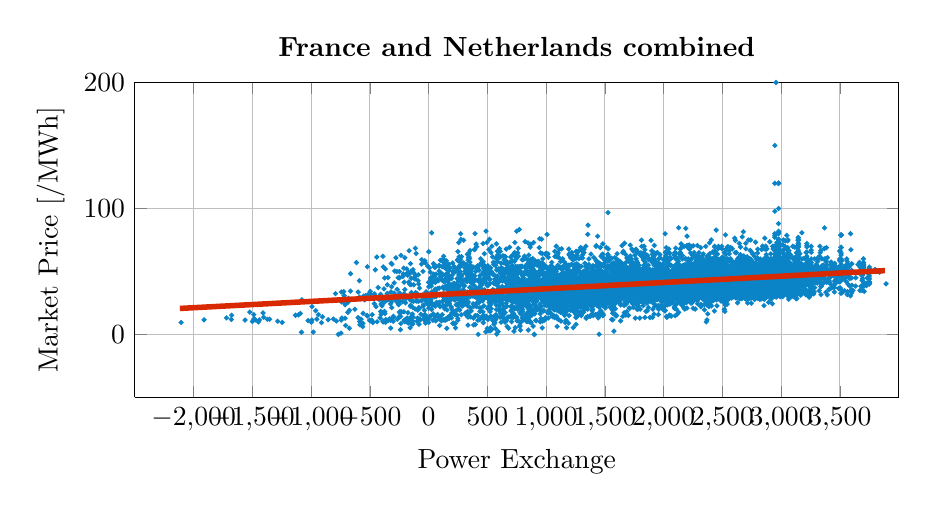
\begin{tikzpicture}

\begin{axis}[%
width=\fwidth,
height=\fheight,
at={(0\fwidth,0\fheight)},
clip mode=individual,
scale only axis,
separate axis lines,
every outer x axis line/.append style={black},
every x tick label/.append style={font=\color{black}},
xmin=-2500,
xmax=4000,
xlabel={Power Exchange},
xmajorgrids,
xtick={-2000,-1500,-1000,-500,0,500,1000,1500,2000,2500,3000,3500},
every outer y axis line/.append style={black},
every y tick label/.append style={font=\color{black}},
ymin=-50,
ymax=200,
ylabel={Market Price [\euro/MWh]},
ymajorgrids,
title style={font=\bfseries},
title={France and Netherlands combined}
]
\addplot [color=mycolor1,line width=1.0pt,mark size=0.3pt,only marks,mark=*,mark options={solid},forget plot]
  table[row sep=crcr]{%
239	15.15\\
-183	12.96\\
-266	12.09\\
-69	11.7\\
-365	11.66\\
-483	11.35\\
-475	9.85\\
-1246	9.54\\
-2107	9.49\\
-1911	11.64\\
-1679	11.94\\
-1720	13.15\\
-1677	15.24\\
-1404	13.69\\
-1485	12.43\\
-1448	9.92\\
-1353	12.12\\
-1133	15.24\\
-1488	15.73\\
-1522	17.73\\
-1107	15.63\\
-903	13.93\\
-525	15.1\\
-94	12.95\\
-366	9.62\\
-585	7.64\\
-675	4.96\\
-768	0.06\\
-746	1.05\\
-706	7.08\\
-332	12.5\\
-314	21.31\\
34	30.44\\
165	35.48\\
333	33.06\\
462	33.78\\
397	37.97\\
429	37.42\\
411	36.24\\
528	32.18\\
757	33.56\\
369	52.94\\
353	66.7\\
410	53.53\\
287	39.54\\
56	35.9\\
295	35.47\\
236	30.64\\
20	27.4\\
24	25.23\\
-30	15.63\\
-236	8.74\\
-209	11.28\\
89	12.34\\
-223	26.02\\
165	31.66\\
415	31.96\\
367	31.94\\
628	30.96\\
695	31.45\\
508	39.05\\
438	30.99\\
303	30.46\\
319	30.43\\
406	31.12\\
780	36.98\\
200	34.97\\
330	42.18\\
66	30.39\\
-128	26.32\\
457	31.82\\
593	32.22\\
505	11.94\\
831	10.5\\
397	7.93\\
229	5.23\\
155	4.86\\
211	8.96\\
-559	8.72\\
-388	9.91\\
132	11.5\\
472	12.76\\
517	13.36\\
623	14.03\\
278	15.64\\
582	14.24\\
1087	14.48\\
1599	30\\
1341	12.86\\
1159	16.79\\
645	21.08\\
523	18.1\\
235	16.14\\
677	13.84\\
819	14.89\\
1012	17.34\\
1057	15.46\\
869	14.69\\
1071	13.33\\
854	10.96\\
787	9.83\\
806	11.66\\
-346	11\\
-354	11.38\\
-132	13.77\\
295	27.42\\
398	30.9\\
458	32.45\\
465	32.07\\
651	29.91\\
837	28.41\\
892	16.89\\
880	15.39\\
1599	46.14\\
1272	40.13\\
1147	38.49\\
848	34.67\\
465	29.4\\
583	28.81\\
706	22.08\\
335	13.84\\
-24	11.89\\
-182	9.85\\
-323	5.09\\
-240	3.79\\
-134	8.24\\
778	17.29\\
1361	48.6\\
1004	46.6\\
1222	40\\
1730	67.8\\
1761	67.3\\
1599	46.08\\
1599	46.08\\
1577	34.5\\
1599	46.08\\
1612	48.99\\
2128	84.71\\
1526	54.57\\
1055	50.7\\
1349	41.75\\
930	28.34\\
1299	38.52\\
1124	33.69\\
564	9.26\\
858	9.98\\
536	3.88\\
422	0.07\\
486	2.05\\
890	6.52\\
1126	26.07\\
1599	34.99\\
1399	49.42\\
753	52\\
596	52\\
359	54.36\\
182	52.78\\
689	49.99\\
933	45.93\\
1180	43\\
1173	46\\
1151	54.44\\
1075	61.93\\
657	56.29\\
998	40.02\\
1159	31.58\\
1304	36.08\\
1056	33.51\\
846	22.01\\
1068	14.61\\
956	12.67\\
826	11.34\\
950	9.99\\
1249	22.41\\
1217	30.31\\
915	46.42\\
1430	57.96\\
1123	57.82\\
980	53.7\\
844	54.51\\
1330	56.46\\
1436	54.3\\
1511	51.11\\
1642	47\\
1765	52.06\\
1833	70.01\\
1773	65\\
1225	61.89\\
1442	48.39\\
1413	38.97\\
1561	39.86\\
1236	38.79\\
787	27.18\\
991	26.5\\
660	24.83\\
440	18.34\\
473	12.96\\
820	25.04\\
920	34.65\\
1032	48\\
966	56.97\\
348	48.54\\
375	46.99\\
370	47.38\\
672	48.92\\
861	46.65\\
836	41.82\\
902	37.84\\
1066	43.83\\
731	52.66\\
764	62.06\\
270	59.78\\
44	47.89\\
922	40.66\\
1274	45.35\\
1123	44.29\\
939	42.64\\
1049	38\\
1248	32.2\\
1163	16.27\\
1260	15.49\\
1648	33.77\\
1631	46.7\\
1831	62.87\\
1889	59.51\\
1474	61.62\\
1236	59.99\\
1509	58.32\\
938	57.73\\
1290	53.76\\
1462	50.84\\
1552	46.87\\
1683	53.65\\
1811	74.86\\
1658	66.02\\
1094	61.5\\
552	57.3\\
688	46.82\\
882	50\\
949	47.33\\
1072	40.36\\
634	28.17\\
1346	35.03\\
1217	28.26\\
1109	26.76\\
1116	28.27\\
997	34.12\\
22	38.34\\
896	43.65\\
757	45\\
863	46.36\\
800	46.34\\
706	49.72\\
749	41.89\\
710	37.94\\
827	38.34\\
1112	40.28\\
1537	51.79\\
1230	59.12\\
903	58.65\\
429	50.94\\
901	44.8\\
1260	52.81\\
655	48.69\\
1204	43.47\\
969	40\\
715	25.86\\
611	16.97\\
1373	14.51\\
1256	16.47\\
1392	16.18\\
1404	23.1\\
1318	31.5\\
1768	44.33\\
787	25.75\\
624	23.98\\
522	29.73\\
405	24.67\\
1159	25.7\\
1223	27.07\\
834	31.11\\
1224	39.66\\
963	41.96\\
642	46.09\\
351	37.35\\
66	32.85\\
120	37.62\\
781	32.17\\
526	26\\
1040	27.86\\
790	27.6\\
633	13.45\\
738	14.24\\
1032	26.71\\
1367	33.11\\
1581	50.84\\
1446	51.45\\
1446	53.89\\
2027	64.36\\
2018	65.14\\
1775	55.89\\
1791	55\\
1751	54.94\\
1832	54.97\\
1906	57.93\\
1767	67.48\\
1828	64.41\\
1311	60.71\\
1236	51.62\\
1372	44.67\\
1731	43.21\\
2077	43.21\\
825	31.14\\
126	29.65\\
927	29.56\\
780	24.17\\
860	19.72\\
1207	30.34\\
883	36.98\\
1279	60.09\\
1073	65.94\\
1255	66.06\\
1285	66.95\\
1322	67.51\\
1140	60.02\\
1204	55.01\\
1541	52.54\\
1564	51.86\\
1648	55.88\\
1921	70.68\\
1528	68\\
1403	53.7\\
1573	54.94\\
1222	45.14\\
1470	44.94\\
1310	39.99\\
1194	33.03\\
992	30.66\\
876	29.92\\
744	29.63\\
600	29.54\\
983	30.65\\
1215	39.94\\
1217	55.67\\
756	62.65\\
731	58.07\\
940	55.47\\
943	53.9\\
794	54.16\\
823	54.35\\
866	50.75\\
945	50.51\\
1010	52.1\\
965	56.49\\
852	62.96\\
1019	61.29\\
1161	47\\
1104	38.6\\
861	39.46\\
825	35.75\\
688	30.06\\
983	28.92\\
1014	25.6\\
841	21.42\\
891	18.42\\
1151	28.66\\
961	33.35\\
1588	50.09\\
1193	48.34\\
967	51.57\\
831	50.84\\
977	52.2\\
1085	51.52\\
1648	55\\
1600	54.94\\
1771	53.62\\
1837	55\\
2012	79.94\\
1364	55.55\\
1174	55\\
1241	46.02\\
1032	35.23\\
1196	37.69\\
2024	38\\
897	29.53\\
1399	28.17\\
1073	19.58\\
912	11.23\\
984	11.18\\
917	20.74\\
1078	34.03\\
867	48.97\\
666	49.96\\
1091	47.71\\
1069	47.91\\
927	47.96\\
948	48.68\\
1109	46.17\\
1239	42.32\\
1312	47.44\\
1465	48.87\\
1461	68.99\\
1097	52.75\\
889	49.43\\
1021	43.74\\
1048	33.33\\
1433	34.45\\
1340	35.9\\
1146	30.5\\
680	29.79\\
1010	28.58\\
1218	26.79\\
1109	18.63\\
954	22.25\\
191	22\\
238	30.25\\
513	33.34\\
896	39.96\\
859	35.17\\
721	32.44\\
456	31.28\\
527	30.89\\
740	30.68\\
901	30.88\\
1362	33.17\\
1399	54.53\\
1399	45.05\\
1151	39.72\\
1178	30.21\\
925	28.63\\
1044	30.4\\
1327	38.63\\
887	36.1\\
389	30.14\\
1074	26.15\\
871	9.48\\
847	12.8\\
903	16.41\\
-17	12.18\\
77	15.76\\
441	29.99\\
809	37.57\\
1125	44.38\\
1228	46.47\\
1287	49.96\\
1360	44.12\\
1417	35.64\\
1516	27.42\\
1518	29.67\\
1687	60.71\\
1599	60\\
1524	46.54\\
1289	42.51\\
1379	40.02\\
1530	41.86\\
1660	38\\
1739	34.75\\
1815	29.46\\
1741	29.21\\
1599	14.99\\
1633	29.33\\
1320	25.5\\
1840	45.93\\
2148	71.97\\
1716	70.92\\
2033	64.5\\
2088	62.93\\
2102	64.44\\
1874	59.61\\
2344	58.04\\
2327	54.16\\
2390	49.7\\
2405	52.53\\
2516	64.91\\
2199	77.99\\
1809	63.97\\
1863	62.7\\
1467	50.4\\
1771	58.17\\
1720	49.38\\
1711	44.79\\
1763	34.35\\
2071	30.65\\
2009	30.3\\
1959	30.65\\
2263	33.68\\
1917	45.86\\
2409	59.91\\
1754	62.98\\
1251	60.19\\
1095	63.32\\
1312	65.65\\
1264	62.91\\
1530	61.46\\
1614	57.41\\
1707	50.81\\
1747	54.09\\
2187	60.23\\
1556	60.57\\
1527	62.97\\
1522	52.97\\
989	48.03\\
1135	51.45\\
1314	47.44\\
1311	45.67\\
1712	43.09\\
1391	34.97\\
1272	31.02\\
1300	31.14\\
964	35.41\\
1008	48.5\\
1111	67.49\\
-166	66.49\\
1	65.66\\
-202	60.88\\
-235	62.79\\
-441	61.44\\
-58	59.37\\
244	58.96\\
458	54.76\\
544	61.62\\
866	71.58\\
395	80.06\\
474	64.04\\
649	62\\
382	53.5\\
654	61.58\\
863	53.5\\
1074	41.81\\
1727	41.5\\
1748	39.22\\
1603	31.32\\
1661	31.17\\
1668	34.03\\
1775	43.13\\
2115	60.59\\
1219	65.1\\
1266	65.05\\
1264	64.92\\
1233	62.17\\
1208	60.92\\
1584	60.91\\
1594	54.77\\
1717	49.69\\
1704	48.08\\
1727	55.17\\
1197	63.96\\
862	57.53\\
775	53.78\\
650	45.45\\
875	53.8\\
1205	46.91\\
556	35.05\\
1162	32.29\\
1035	30.34\\
1039	29.99\\
1137	30.53\\
806	32.17\\
1372	43.42\\
1238	61.6\\
632	62.5\\
717	63.3\\
611	61.59\\
590	63.28\\
574	60.39\\
644	59.33\\
850	58.97\\
839	53.19\\
953	53.03\\
998	64.41\\
531	64.94\\
330	63.71\\
418	54.64\\
487	50.15\\
933	47.09\\
914	49\\
1264	37.68\\
804	32.05\\
671	31.1\\
1248	30.32\\
1170	29.83\\
1076	29.04\\
1300	30.9\\
568	31.58\\
905	39.27\\
1033	42.04\\
1162	43.63\\
1116	44.11\\
928	45.82\\
998	37.68\\
829	32.69\\
810	32.69\\
848	33.57\\
1119	38.13\\
922	48.04\\
916	43.14\\
526	32.57\\
188	30.05\\
413	32.86\\
662	38.23\\
126	22.11\\
-36	19.14\\
-42	14.85\\
4	13.14\\
-24	13.22\\
174	12.73\\
0	9.53\\
6	14.05\\
53	14.04\\
383	22.19\\
470	22.69\\
332	22.85\\
-45	23.42\\
205	19.08\\
-29	15.23\\
-153	12.89\\
-143	8.26\\
344	17.66\\
-47	22.42\\
-61	26.7\\
467	31.96\\
244	23.75\\
565	28.24\\
599	20.29\\
1	12.63\\
128	11.74\\
248	12.81\\
94	7.1\\
205	8.77\\
633	13.09\\
681	30.14\\
885	47.43\\
580	51.07\\
331	52.47\\
263	53.47\\
146	52.73\\
304	56.05\\
244	50.71\\
351	51.92\\
417	51.92\\
502	51.47\\
167	55.53\\
272	79.92\\
-106	64.25\\
282	47.25\\
12	38.71\\
236	40.2\\
149	38.51\\
367	36.41\\
550	32.92\\
669	30.28\\
601	29.57\\
603	30.16\\
920	31.21\\
657	41.47\\
846	55.05\\
456	56.58\\
504	54.52\\
508	52\\
468	52.44\\
353	49.94\\
733	47.44\\
876	46.5\\
949	48\\
1013	49.77\\
666	57.75\\
538	70\\
127	62.09\\
282	56.94\\
142	47.4\\
255	53.42\\
263	48.28\\
885	38.65\\
982	30.54\\
889	29.63\\
725	28.98\\
700	29.55\\
961	31.08\\
936	37.1\\
961	55.38\\
697	52.95\\
683	52.9\\
351	57.44\\
294	56.78\\
59	53.55\\
366	54\\
533	50.01\\
851	47.44\\
1005	47.02\\
698	61.52\\
772	83.27\\
495	72.99\\
261	54.43\\
350	49.5\\
786	54.11\\
888	52.05\\
806	37.75\\
1210	34.94\\
1075	34.29\\
1102	29.92\\
1183	30.32\\
729	34.43\\
1190	45.2\\
1385	53.07\\
476	54.73\\
952	64.78\\
832	59.99\\
967	64.16\\
743	59.72\\
980	54.48\\
1140	51.89\\
1266	51.5\\
1352	51.56\\
1487	55.12\\
1131	67.98\\
810	59.67\\
1066	50.5\\
721	45.81\\
1363	46.52\\
1400	47.1\\
1497	42.96\\
1431	42.5\\
1595	36.54\\
1463	33.06\\
1580	31.95\\
1817	40.03\\
1514	46.9\\
1425	69.94\\
577	71.95\\
463	72.19\\
609	65.88\\
339	60.93\\
7	52.93\\
463	48.14\\
328	45\\
268	44.1\\
337	44.23\\
403	52.92\\
260	61.76\\
-318	56.35\\
-172	49.08\\
-160	40\\
162	41.99\\
211	39.17\\
201	31.04\\
-254	28.94\\
-140	26.63\\
2	20.87\\
-115	20.18\\
-77	20.71\\
122	26.82\\
-680	28.7\\
-429	37.27\\
-90	42.65\\
17	43.28\\
16	44.55\\
-123	48.59\\
-159	40.24\\
-293	32.87\\
-247	32.8\\
-147	33.28\\
76	43.56\\
-48	50.02\\
-248	44.94\\
57	41.24\\
-268	35.81\\
53	35.01\\
235	35.96\\
-169	41.62\\
-512	31.96\\
-741	25.8\\
-93	19.38\\
-158	13.18\\
-142	14.07\\
-372	16.54\\
-961	18.85\\
-993	22.07\\
-719	30.83\\
-464	31.96\\
-496	31.82\\
-496	34.15\\
-460	32.14\\
-537	30.8\\
134	31.03\\
668	32.95\\
160	36.15\\
158	48.68\\
143	54.57\\
125	53.78\\
51	45.76\\
329	49.81\\
343	48.84\\
195	44.37\\
2	37.8\\
675	36\\
453	31.56\\
517	31.52\\
912	36.19\\
1037	54.1\\
1483	71.89\\
893	72.94\\
513	67.5\\
268	57.18\\
281	54.63\\
351	52.9\\
742	51.96\\
908	46.82\\
1100	47.14\\
1227	46.76\\
1297	54.09\\
1193	67.8\\
888	59.96\\
931	57.98\\
497	48.72\\
623	52.2\\
659	52.27\\
677	44.42\\
619	44.96\\
808	40.9\\
696	30.63\\
684	30\\
125	32.38\\
508	47.13\\
348	60.3\\
-32	58.49\\
48	53.88\\
356	51.99\\
529	52.83\\
434	54.68\\
582	51.68\\
833	48.05\\
903	47.59\\
967	48.03\\
1179	53.05\\
1015	63.99\\
554	55.73\\
631	48\\
554	41.26\\
693	44.08\\
772	42.46\\
298	30.53\\
-103	29.98\\
476	28.99\\
300	25.71\\
332	18.11\\
621	28.08\\
374	33.51\\
-346	45.16\\
-271	49.94\\
-211	52.61\\
149	58.57\\
90	54.16\\
-191	48.08\\
146	52.2\\
307	50.09\\
514	43.92\\
698	42.55\\
705	49.69\\
391	67.38\\
51	53.32\\
-78	36.79\\
-614	57.1\\
-368	52\\
-260	45\\
842	42.28\\
691	39.94\\
482	34.79\\
416	28.27\\
500	28.67\\
-7	32.2\\
486	44\\
171	55.87\\
204	56.7\\
100	58.84\\
279	61.77\\
256	60.43\\
126	57.28\\
665	55.91\\
983	55.29\\
1084	49.94\\
1085	47.89\\
884	55.89\\
586	66.01\\
443	60.02\\
96	48.05\\
230	37.12\\
588	33.71\\
828	39.61\\
256	23.64\\
633	19.51\\
342	14.66\\
159	12.18\\
226	8.54\\
187	15.42\\
505	30.68\\
546	47.79\\
485	45.71\\
555	47.63\\
800	47.94\\
1040	51.34\\
816	48.37\\
854	42.94\\
851	36.86\\
831	32.31\\
916	31.3\\
1205	36.16\\
884	59.92\\
568	54.71\\
676	43.31\\
377	30.49\\
864	38.37\\
909	40.84\\
325	28\\
-241	26.43\\
269	25.9\\
-18	24.93\\
-133	10.52\\
-139	16.2\\
73	24.04\\
-752	27.13\\
-512	29.51\\
-160	29.48\\
190	28.07\\
270	26.76\\
210	28.03\\
292	25.5\\
176	25.96\\
886	28.81\\
687	28.03\\
211	31.17\\
255	42.58\\
-22	33.88\\
-419	27.57\\
-324	24.29\\
-160	27.55\\
235	23.6\\
-239	14.23\\
-738	13.02\\
-710	12.87\\
-855	11.77\\
-997	9.72\\
-912	9.36\\
-785	10.63\\
-1285	10.54\\
-1026	11.04\\
-674	19.16\\
-399	17.7\\
-176	17.29\\
62	14.68\\
194	13.16\\
-25	10.5\\
-27	8.97\\
-82	12.42\\
15	14.69\\
404	35.79\\
140	36.81\\
192	31.23\\
-160	27.97\\
49	30.04\\
515	25.31\\
808	36.13\\
918	33.87\\
752	27.22\\
530	23.86\\
-153	23.08\\
1173	33.18\\
1164	45.43\\
1883	59.42\\
1826	60.99\\
1614	58.79\\
972	60.02\\
897	54.96\\
841	56.12\\
1570	56.82\\
1603	55.63\\
1685	51.47\\
1710	47.44\\
1847	54.94\\
1354	79.49\\
1044	54.32\\
1326	50.06\\
1180	46.57\\
1417	47.59\\
1594	42.83\\
1205	30.75\\
1487	32.07\\
1203	29.45\\
1018	28.27\\
970	28.05\\
1015	30.72\\
880	41.12\\
343	53.8\\
324	55.34\\
447	56.62\\
215	54.1\\
338	51.74\\
171	50.38\\
465	49.25\\
630	42.49\\
722	39.56\\
785	41\\
737	51.9\\
650	58.97\\
391	67.49\\
205	50\\
392	46.48\\
902	49.48\\
985	44.09\\
1090	45\\
886	41.94\\
698	37.84\\
549	28.43\\
580	29.36\\
128	36.72\\
509	45.54\\
797	59.3\\
249	65.77\\
-113	68.42\\
-278	60.87\\
-312	55.9\\
-289	50.33\\
251	49.42\\
277	45.92\\
384	43.34\\
675	40.93\\
478	44.99\\
336	58.94\\
-8	54.37\\
-186	52.03\\
55	42.78\\
338	46.13\\
631	44.03\\
610	42.97\\
730	34.54\\
485	32.23\\
437	18.33\\
498	12.47\\
-97	26.67\\
443	42.44\\
-60	55.88\\
153	53.54\\
465	57.79\\
642	56.72\\
909	57.98\\
922	55\\
1243	52.89\\
1178	52.35\\
1226	45.25\\
1427	42.91\\
1228	48.66\\
941	68.92\\
711	58.69\\
309	52.81\\
385	42\\
1004	40.63\\
940	38.04\\
1579	33\\
1549	32.72\\
1364	29.33\\
1237	24.42\\
1329	25.63\\
842	29.44\\
1380	46.4\\
1213	61.12\\
758	64.8\\
689	69.25\\
583	62.12\\
570	55\\
697	52.08\\
1024	47.1\\
1020	44.22\\
1079	36.2\\
1115	40\\
1019	46.18\\
682	53.48\\
781	48.73\\
955	36.97\\
694	30.39\\
1256	30.61\\
1702	42.44\\
253	27.73\\
-210	17.99\\
148	12.38\\
-99	10.36\\
-203	10.11\\
-157	10.33\\
143	11.36\\
-600	13.34\\
-375	18.26\\
-397	22.66\\
35	23.11\\
1	23.08\\
-256	23.76\\
-155	22.48\\
193	21.11\\
264	19.33\\
257	20.46\\
149	27.73\\
190	39.29\\
-124	44.85\\
-270	28.93\\
-328	29.36\\
-208	41.5\\
132	41.56\\
0	25.49\\
-300	14.46\\
-22	12.35\\
-173	9.06\\
-157	5.3\\
-82	8.08\\
-13	11.12\\
-475	9.53\\
-497	10.73\\
-301	13.37\\
-242	16.81\\
-248	17.86\\
-409	18.23\\
-414	13.15\\
-503	11.38\\
-301	10.48\\
-42	12.22\\
322	15.26\\
718	40.15\\
813	47.98\\
733	46.83\\
646	34.73\\
967	39.08\\
1086	31.53\\
756	31.59\\
1090	25.69\\
1003	23.33\\
889	17.52\\
920	19.63\\
1314	26.47\\
1125	43.79\\
1426	58.75\\
1141	53.31\\
796	54\\
791	49.32\\
1059	50\\
764	44.22\\
949	42.07\\
984	34.96\\
1315	37.25\\
556	40.33\\
579	43.03\\
488	82.04\\
404	71.74\\
618	56.51\\
351	47.19\\
772	49.94\\
803	43.43\\
707	31.95\\
1039	31.66\\
801	30.09\\
686	28.86\\
764	29.2\\
587	31.3\\
732	42.03\\
42	56.19\\
90	54.9\\
114	53.79\\
362	51.9\\
643	50.74\\
594	51.42\\
705	48.48\\
801	43.27\\
944	43.44\\
1013	45.72\\
1244	53.91\\
821	73.68\\
588	59.98\\
725	45.94\\
580	39.68\\
781	41.9\\
809	36.47\\
920	32.16\\
1182	29.65\\
960	28.46\\
864	27.67\\
971	28.51\\
541	29.34\\
1240	38.19\\
885	47.45\\
676	49.44\\
751	52.21\\
759	53.93\\
1053	53.96\\
878	50.76\\
1269	49.48\\
1198	49.37\\
1240	47.95\\
1284	44.71\\
1387	47.44\\
1086	70\\
869	59.54\\
978	54.27\\
894	47.02\\
1273	44.18\\
1213	44.96\\
1003	31.28\\
1508	29.47\\
1145	28.87\\
856	27.75\\
817	25.59\\
152	27.85\\
891	34.51\\
585	46.28\\
714	48.34\\
793	48.28\\
902	44.93\\
1329	46.95\\
1247	47.58\\
1318	44.94\\
1424	40.02\\
1505	34.96\\
1497	32.45\\
1599	41.78\\
1475	55\\
1169	52.17\\
1119	47.44\\
922	39.95\\
1266	41.78\\
1376	41.49\\
1338	32.91\\
1388	22.15\\
1151	20.84\\
1026	19.42\\
1108	21.02\\
534	26.64\\
1311	35.83\\
1162	46.31\\
1169	49.03\\
1107	52.95\\
1317	50.07\\
1473	48.45\\
1117	42.88\\
1264	37.61\\
1143	32.16\\
1155	32.1\\
1227	31.68\\
1193	42.9\\
1690	49.44\\
1013	49.96\\
681	49.08\\
447	40.71\\
903	40.93\\
994	41\\
581	35.11\\
220	29.96\\
117	26.09\\
447	21.02\\
362	18.67\\
356	21.15\\
587	27.93\\
-169	29.38\\
169	32.92\\
601	37.43\\
904	37.35\\
1045	36.86\\
971	38.85\\
797	35.47\\
771	29.59\\
620	31.99\\
586	31.33\\
846	37.71\\
723	50.91\\
618	53.1\\
177	44.22\\
90	36.72\\
209	40.34\\
740	36.96\\
436	26.11\\
-137	21.63\\
98	22.07\\
157	19.48\\
40	16.28\\
26	19.86\\
116	15.73\\
-938	15.73\\
-1409	17.1\\
-1092	16.63\\
-688	17.46\\
-558	16.77\\
-521	14.68\\
382	12.98\\
249	11.26\\
335	7.45\\
110	10.84\\
37	11.28\\
378	24.31\\
474	35.49\\
603	27.81\\
398	23.11\\
524	27.1\\
620	25.71\\
-40	14.5\\
415	15.09\\
197	17.22\\
98	13.68\\
167	14\\
-234	18.12\\
455	35.66\\
482	46.95\\
399	50\\
436	46.65\\
577	45.98\\
452	41.79\\
25	40.46\\
578	39.32\\
832	35.99\\
1056	31.07\\
1260	32.97\\
1299	46.16\\
1322	64.95\\
1103	64.73\\
822	48.99\\
586	35.43\\
791	37.44\\
789	33.87\\
153	26.22\\
153	23.87\\
287	22.77\\
137	20.29\\
234	18.97\\
609	25.94\\
778	36.97\\
994	46.95\\
363	46.66\\
102	46.12\\
-148	44.59\\
-116	44\\
153	44.94\\
522	40.49\\
700	36.09\\
976	35.3\\
1089	33.71\\
922	42.61\\
846	72.68\\
729	62.52\\
198	46.87\\
506	39.88\\
612	42.89\\
761	39.59\\
1122	36.05\\
1090	30\\
801	27.29\\
696	26.91\\
797	27.86\\
306	28.48\\
1058	39.22\\
649	45.05\\
614	49.24\\
1031	51.3\\
901	50.42\\
823	50\\
692	46.91\\
720	46.42\\
678	44.96\\
796	43.35\\
441	41.81\\
564	43.99\\
865	71.19\\
734	72.95\\
268	49.85\\
276	45.59\\
769	42.44\\
1099	40.05\\
971	33.99\\
1103	32.03\\
781	30.28\\
583	29.61\\
462	29.48\\
280	32.18\\
459	41.54\\
497	53.34\\
-151	50.1\\
-179	47.1\\
-216	48.14\\
-219	46\\
144	44.24\\
370	44.81\\
402	43.22\\
577	41.94\\
696	40.62\\
707	51.76\\
732	64.96\\
657	57.83\\
460	48.66\\
728	43.21\\
986	41.45\\
911	40.16\\
816	36.25\\
1229	34.94\\
1030	30.19\\
966	28.03\\
991	28.54\\
352	29.94\\
886	39.6\\
327	47.45\\
352	49.45\\
531	49.77\\
865	49.12\\
976	47.42\\
1134	46.72\\
1166	44.7\\
1136	42.31\\
1117	41.92\\
1078	42.98\\
986	47.3\\
343	64.68\\
123	59.92\\
256	47.28\\
224	39.75\\
473	42.95\\
574	42\\
491	40.61\\
605	35.72\\
679	33.79\\
510	30.22\\
462	29.28\\
478	29.33\\
-433	28.98\\
-320	33.71\\
-351	39.51\\
-87	47.4\\
90	50.34\\
114	48.18\\
507	47.97\\
350	43.25\\
171	38.63\\
128	36.46\\
26	33.77\\
-1	41.27\\
338	63.21\\
298	74.76\\
-113	45.93\\
83	42.66\\
357	48.38\\
485	44.97\\
189	44.94\\
-151	39.4\\
-208	32.28\\
5	29.31\\
-273	27.57\\
-341	27.86\\
-282	27.33\\
-808	27.04\\
-1079	27.49\\
-793	32.39\\
-743	33.69\\
-599	33.67\\
-665	34.38\\
-544	27.45\\
-711	23.55\\
-704	24.59\\
-688	25.42\\
-603	28.22\\
-723	33.96\\
-589	42.62\\
-127	39.44\\
-409	31.89\\
-380	36.16\\
-353	32.59\\
-729	26.52\\
-196	25.11\\
-405	24.08\\
-448	22.14\\
-251	24.03\\
-358	27.01\\
94	43.93\\
-249	49.94\\
-454	51.33\\
-386	53.68\\
-134	51.43\\
138	57.13\\
-166	47.83\\
14	49.41\\
110	46.48\\
498	38.95\\
590	40.98\\
724	44.96\\
257	72.91\\
26	80.69\\
63	47.81\\
24	43.99\\
480	45.3\\
463	43.34\\
1066	45.03\\
1088	39.19\\
1120	33.29\\
1051	28.99\\
1168	29.68\\
865	33.28\\
802	47.18\\
999	53.9\\
588	57.9\\
691	57.32\\
595	51.02\\
634	51.98\\
828	52.3\\
965	50\\
947	48.59\\
1040	46.51\\
1138	45.92\\
1244	45.87\\
961	75.64\\
1008	79.38\\
712	54.77\\
739	50.68\\
1039	49.01\\
948	50.54\\
724	40.21\\
375	39.94\\
821	42.1\\
842	34.72\\
961	33.37\\
1063	41.28\\
746	47.32\\
815	62.16\\
660	67.76\\
603	68.08\\
784	53.01\\
635	44.96\\
434	43.85\\
437	44.19\\
579	40.21\\
890	38.02\\
1015	38.08\\
1031	46.54\\
706	58.03\\
763	68.37\\
976	49.04\\
730	42.58\\
898	45.99\\
716	44.1\\
757	37.43\\
710	36.72\\
546	34.14\\
642	28.81\\
765	29.19\\
909	33.98\\
586	42.85\\
48	55.33\\
-29	56.97\\
-154	56.22\\
364	50\\
316	48.58\\
41	46.41\\
19	44.92\\
219	40.51\\
569	34.11\\
637	37\\
863	45\\
344	61.59\\
409	69.75\\
832	53.9\\
318	42.17\\
369	45.73\\
281	40.97\\
-85	40.01\\
403	33.98\\
-96	32.22\\
152	28.9\\
215	29.1\\
331	32.06\\
-293	40.9\\
-664	48.26\\
-521	53.76\\
-389	62\\
-130	49.17\\
-248	45.36\\
-374	44.82\\
-315	37.93\\
-203	35.64\\
160	31.97\\
337	31.94\\
452	39.36\\
171	47.09\\
219	49.26\\
378	45.95\\
24	41.92\\
242	44.28\\
523	43.68\\
177	39.97\\
-110	33.31\\
-554	30.44\\
-267	25.71\\
-383	24.96\\
-316	25.82\\
-390	26.92\\
-588	29.6\\
-142	31.96\\
-47	31.51\\
-197	28.19\\
-379	26.17\\
-462	24.42\\
-628	20.02\\
-404	15.91\\
-193	12.03\\
220	16.02\\
667	22.55\\
662	35.58\\
296	42.77\\
-108	30.03\\
-263	25.14\\
68	25.47\\
27	23.65\\
-480	15.67\\
-253	13.75\\
-575	12.1\\
-744	11.4\\
-1500	10.35\\
-1491	11.4\\
-994	11.49\\
-1562	11.4\\
-1473	11.55\\
-1372	12.05\\
-1440	11.54\\
-952	12.11\\
-810	12.26\\
-587	10.29\\
-561	6.2\\
-1082	1.75\\
-981	1.87\\
-579	9.83\\
58	22.41\\
354	41.73\\
257	34.86\\
-35	28.07\\
54	30.09\\
-22	26.92\\
328	24.26\\
287	22.62\\
124	22.73\\
144	22.76\\
407	22.11\\
90	25.57\\
1008	43.5\\
917	48.28\\
615	48.12\\
364	44.76\\
365	40.9\\
203	37.42\\
76	36.46\\
172	35.85\\
240	33.8\\
431	30.13\\
657	30.19\\
955	36.36\\
850	56.07\\
276	75.46\\
111	46.32\\
306	38.68\\
391	35.17\\
402	30.93\\
338	25.83\\
532	25.9\\
263	24.63\\
173	24.27\\
306	23.78\\
-105	26.5\\
547	35.08\\
458	42.55\\
487	44.58\\
443	40.03\\
1015	40.2\\
873	36.07\\
519	31.88\\
445	30.65\\
623	28.18\\
755	28.72\\
892	30.91\\
1183	36.26\\
1240	49.94\\
740	54.1\\
1058	42.56\\
709	34.04\\
802	40.03\\
771	32.99\\
273	28.87\\
672	28.04\\
460	26.65\\
428	25.15\\
564	25.69\\
688	28.09\\
866	35.8\\
474	44.54\\
316	43.73\\
805	41.27\\
552	32.59\\
329	33.67\\
190	30\\
260	28.78\\
462	28.42\\
691	29.25\\
876	30.79\\
1299	37.04\\
1014	49\\
945	75.98\\
853	48.43\\
816	42.01\\
1076	38.28\\
1047	32.08\\
1132	31.35\\
228	30.65\\
810	29.96\\
692	30\\
713	30.11\\
480	31.43\\
1348	43.03\\
1127	53.46\\
891	49.84\\
441	41.27\\
400	34.74\\
152	29.77\\
-73	30.58\\
-31	28.42\\
9	28.78\\
160	30.95\\
292	35.54\\
567	30.84\\
222	52.76\\
517	75.55\\
614	48.69\\
893	43.63\\
1261	42.87\\
1141	40.69\\
776	34.96\\
1011	32.01\\
1186	30.99\\
1097	29.57\\
1243	29.65\\
586	32.89\\
1184	42.04\\
729	49.94\\
757	47.93\\
835	42.94\\
1387	41.26\\
1191	38.83\\
912	37.01\\
888	34.91\\
781	30.96\\
878	29.53\\
973	30.91\\
1239	37.91\\
1294	45.07\\
1335	53.95\\
1574	49.94\\
1395	38.64\\
1620	42.44\\
1684	38.99\\
902	28.64\\
602	18.86\\
436	21.1\\
419	11.3\\
383	7.58\\
435	11.81\\
446	13.36\\
536	14.02\\
870	22.83\\
1353	20.01\\
1394	16.52\\
1423	15.8\\
1266	21.57\\
1157	15.2\\
1096	12.55\\
1107	11.78\\
1169	11.26\\
1466	18.81\\
1601	44.94\\
1599	48\\
1469	25.54\\
1222	23.29\\
1233	20.33\\
977	19.29\\
639	15.89\\
1054	14.23\\
748	13.29\\
571	11.77\\
649	11.11\\
-438	10.12\\
-325	11.23\\
-389	10.91\\
-162	11.44\\
61	10.77\\
149	12.34\\
167	13.02\\
80	13.95\\
546	11.07\\
465	9.33\\
509	3.07\\
738	5.41\\
1163	9.43\\
1122	22.78\\
1611	52\\
1599	49\\
1266	21.31\\
1317	20.51\\
1443	28.62\\
1498	29.73\\
1133	26.33\\
1172	23.93\\
1139	20.73\\
1226	21.96\\
919	26.41\\
1950	42\\
1619	50.81\\
1444	49\\
1449	56.84\\
1828	59.16\\
1785	65.27\\
1593	50\\
1776	50\\
1801	49.96\\
1894	49.08\\
2005	51.87\\
2141	67.78\\
1763	47.44\\
1814	69.94\\
1482	54.86\\
1580	44\\
1624	45\\
1609	44.25\\
1820	31.57\\
2067	32.18\\
1752	29.99\\
1682	24.07\\
1771	24.89\\
2090	28.06\\
1938	40.44\\
1863	49.49\\
1422	50.12\\
1382	63.77\\
1275	55\\
1530	61.99\\
1703	58.13\\
1607	52.24\\
1505	45.13\\
1421	42\\
1383	41.36\\
1578	42.44\\
1437	39.68\\
1178	46.28\\
1112	41.55\\
1100	39\\
1367	32.73\\
1451	30.33\\
1064	22.2\\
1380	22.46\\
1264	14.3\\
1285	22.46\\
1492	29.66\\
1250	27.44\\
1889	42.36\\
2121	49.79\\
1299	47.99\\
1199	48\\
1199	39.01\\
1189	34.72\\
964	33.41\\
912	32.59\\
883	31.48\\
1183	28.19\\
1199	42.44\\
1568	47.59\\
1281	42.44\\
1498	54.97\\
1504	49\\
1500	45\\
1661	44\\
1544	41.93\\
1250	26.47\\
1443	26.72\\
1209	24.54\\
1140	17.18\\
1241	18.05\\
1445	24.57\\
1524	37.54\\
1676	46.15\\
856	41.33\\
917	35.3\\
943	31.3\\
886	29.01\\
555	26.8\\
521	26.56\\
539	25.76\\
850	26.52\\
1024	26.84\\
1223	28.95\\
1064	36.94\\
1139	45.07\\
1399	32\\
1191	27.84\\
1389	31.24\\
1263	30.47\\
1341	21.24\\
995	12.08\\
835	11.32\\
866	10.25\\
1126	10.65\\
978	18.63\\
1588	29.62\\
1688	40\\
1399	39.18\\
1273	38.33\\
1399	44.54\\
1920	63.62\\
1631	57.66\\
1573	55.89\\
1417	45\\
1439	39.96\\
1452	39.94\\
1399	38.93\\
851	42.43\\
953	55\\
689	47.39\\
1084	43.08\\
1309	43.08\\
1192	36.5\\
1094	33.94\\
576	28.54\\
946	24.08\\
703	19.07\\
608	13.66\\
463	17.92\\
802	22.76\\
32	24.31\\
253	29.83\\
671	32.37\\
867	32.33\\
935	32.48\\
936	31.22\\
792	27.59\\
826	27.84\\
796	26.45\\
676	27.99\\
844	31.39\\
626	38.04\\
1030	45.01\\
710	36.93\\
930	31.7\\
1103	30.99\\
1195	24.69\\
706	22.91\\
532	20.54\\
605	20.14\\
502	20.59\\
647	17.65\\
577	19.82\\
313	17.05\\
-66	16.07\\
-83	21.36\\
176	24.42\\
290	26.9\\
369	30.58\\
454	29.26\\
771	24.04\\
826	23.46\\
959	18.55\\
1021	17.34\\
1094	19.29\\
1486	40\\
1350	45.12\\
1299	42\\
1135	37.1\\
1153	40.51\\
1520	35.55\\
1141	32.64\\
1610	30\\
1418	27.8\\
1499	25.08\\
1531	25.3\\
1658	28.82\\
1900	40.58\\
2209	57.32\\
1154	57.52\\
979	54.94\\
1114	42.91\\
1311	42.6\\
1092	43.18\\
1108	44.64\\
1230	43.91\\
1579	41.46\\
1843	40.91\\
2164	40.93\\
1562	47.23\\
1526	96.69\\
1629	48.73\\
1509	41.12\\
1781	44.62\\
1769	41.69\\
1227	37.3\\
669	36.95\\
925	33.3\\
923	30.65\\
970	31\\
1124	35.52\\
1327	42.44\\
258	45\\
968	49.47\\
901	49.99\\
1035	51.15\\
700	45.85\\
480	45.62\\
605	42.97\\
801	42.92\\
928	39.82\\
973	40.1\\
973	44.07\\
1208	49.08\\
749	81.94\\
1199	48.12\\
1252	43.42\\
989	42.8\\
1165	46.99\\
1118	39.53\\
1174	41.02\\
1396	40.42\\
1399	32.22\\
1516	31.13\\
1301	34.68\\
1746	44.49\\
1264	48.93\\
1139	52.06\\
1127	52.07\\
1443	54.01\\
1437	48.32\\
1241	47\\
1381	43.52\\
1379	41.95\\
1695	41.09\\
1823	40.24\\
1927	42.24\\
1645	48.68\\
1357	86.74\\
1467	46.5\\
1655	42.37\\
1780	43.59\\
1653	42.44\\
3268	41.11\\
3252	42.44\\
3584	38.41\\
3611	35.02\\
3707	34.24\\
2921	38.08\\
3445	46.51\\
3484	51.57\\
3368	59.9\\
3254	52.44\\
3556	51.19\\
3435	50.58\\
3050	48.79\\
3052	49.4\\
3089	46.77\\
3374	43.27\\
3552	42.07\\
3746	44.45\\
3179	50\\
2679	81.51\\
2681	62.32\\
2588	46.92\\
3187	48.57\\
3519	45.4\\
3230	40.77\\
2648	41.97\\
3341	41.04\\
3429	37.01\\
3595	35.1\\
3893	40.21\\
3473	45.87\\
3078	51.76\\
2894	58.1\\
2735	57.39\\
2389	47.4\\
2390	45\\
2461	42.06\\
2460	40.59\\
2598	40.81\\
3021	39.99\\
3134	40\\
3407	43\\
3582	44.29\\
2930	70\\
3002	45\\
2991	42.44\\
3166	42.44\\
3039	40.06\\
3106	43.99\\
2731	32.81\\
2548	31.02\\
2602	31.11\\
2558	32\\
2466	31.32\\
2653	36.89\\
2351	39.94\\
2298	43\\
2267	47.44\\
2177	45.62\\
2061	42.62\\
1891	40\\
1773	38\\
1714	34.99\\
1872	34.96\\
2172	39.96\\
2525	43\\
2657	43\\
2340	46.17\\
2867	54.96\\
2806	46\\
2887	44.94\\
2855	40.56\\
2466	44\\
2351	34.94\\
2147	29.49\\
2080	29.49\\
2142	30.7\\
2369	35.04\\
2064	35.04\\
1802	39.33\\
1801	40\\
1732	41\\
1492	38.83\\
1388	37.44\\
1253	36.99\\
1068	32.44\\
1081	30.81\\
1137	31.8\\
1553	39.96\\
1614	39.96\\
2061	45\\
2196	69.97\\
2185	59.94\\
2807	55\\
2356	42.44\\
821	30.91\\
1963	32.46\\
1977	31.28\\
2214	32.2\\
2408	35.77\\
2091	28.14\\
2846	40.69\\
2978	69.53\\
2317	55.47\\
2235	56.01\\
2410	48.33\\
2208	46.08\\
1829	46.7\\
1960	43.73\\
1826	41.79\\
1953	40\\
2144	42.22\\
2370	43.22\\
2498	40.47\\
1771	48.47\\
2606	54.61\\
2904	50\\
2923	44.94\\
2536	44\\
2978	54.48\\
2974	43.64\\
2853	41.06\\
2809	40.5\\
2730	36.26\\
2978	44.94\\
2978	48\\
2675	57.44\\
2271	62.19\\
2473	57.89\\
2600	47.29\\
2720	46.64\\
2525	37.77\\
2742	40\\
2670	39.96\\
2663	38.76\\
2759	39.96\\
2885	42.11\\
2978	73.81\\
2727	50.12\\
2749	45\\
2825	47\\
2978	120\\
2978	120\\
2978	65\\
2815	37.69\\
2889	37.53\\
2906	37.53\\
2949	37.75\\
2655	36.93\\
2978	44\\
2537	49.22\\
2298	62.17\\
2534	54.35\\
2863	48\\
2797	45\\
2528	45\\
2415	44\\
2412	42.12\\
2464	41.19\\
2548	44\\
2748	47.44\\
2978	46\\
2928	52.92\\
2280	58.31\\
2257	53.12\\
2398	44.94\\
2253	40.98\\
2978	34.99\\
2744	31.27\\
2764	31.27\\
2872	32.81\\
2834	28.3\\
2749	29.55\\
2904	38.64\\
2978	55.5\\
2595	52.09\\
2708	49.94\\
2840	50\\
2978	51\\
2777	47.44\\
2701	47\\
2637	44.94\\
2702	44.42\\
2902	45\\
2978	50\\
2978	69.97\\
2897	44.94\\
2741	50\\
2754	47.44\\
2978	63.41\\
2978	64.08\\
2552	37.23\\
2547	34.37\\
2653	34.24\\
2526	30.51\\
2615	30.51\\
2874	31.4\\
2832	37.77\\
2740	46.07\\
2924	51.91\\
2925	56.15\\
2978	63.46\\
2978	120\\
2978	58.9\\
2817	47.44\\
2812	44.94\\
2802	40\\
2859	40\\
2848	40\\
2845	39.94\\
2415	40.99\\
2374	41.76\\
2429	38.72\\
2978	65.37\\
2795	43\\
2792	34.3\\
2766	37.84\\
2622	34\\
2668	34\\
2581	30.74\\
2560	30.74\\
2229	29.5\\
2304	34.44\\
2650	43.18\\
2516	46\\
2476	45\\
2663	47.44\\
2556	42.8\\
2277	35.87\\
2060	34.44\\
2056	34.44\\
2213	33.61\\
2357	35\\
2803	42.44\\
2582	42.44\\
2700	49.99\\
2864	47.44\\
2899	42\\
2745	44.01\\
2113	35.16\\
1919	42.16\\
1890	34.94\\
1778	34.21\\
1813	31.5\\
1853	33.97\\
1280	24.25\\
1190	24.3\\
1197	25.31\\
1343	34.94\\
1361	38.99\\
1497	41.96\\
1743	47.44\\
1470	39.94\\
1367	35.15\\
1349	34.9\\
1418	34.94\\
1353	39.96\\
1669	42.17\\
1928	44.94\\
2103	59.94\\
2057	54.96\\
2046	48\\
2041	35.99\\
2250	29.88\\
2245	27.73\\
2237	28.85\\
2087	29.85\\
2225	29.75\\
2594	29.99\\
2663	41\\
2343	49.94\\
2468	53.05\\
2502	51.06\\
2694	47.45\\
2679	44.61\\
2392	38.94\\
2589	37.09\\
2668	36.16\\
2685	36.26\\
2765	36.31\\
2906	39.12\\
2572	45.31\\
2375	46.99\\
2366	48.75\\
2796	38.58\\
2978	34.86\\
2818	30.07\\
2007	28.01\\
2094	28.01\\
1968	21.92\\
1951	21.44\\
1980	22.69\\
2155	24.02\\
2442	31.84\\
2385	38.99\\
2559	43.96\\
2469	45.8\\
2438	48.41\\
2751	53.7\\
2349	43.88\\
2181	44.6\\
2134	45.32\\
2232	40.42\\
2438	39.94\\
2683	44.46\\
2651	39.94\\
2742	39.96\\
2978	66.56\\
2978	63.54\\
2978	65.06\\
2978	55\\
2804	41.06\\
2818	37.77\\
2928	35.97\\
2826	35.74\\
2973	37.06\\
2978	73.11\\
2978	80.78\\
2911	50.12\\
2720	55.91\\
2853	59.81\\
2738	52.44\\
2650	47.12\\
2398	44\\
2352	44.8\\
2098	41.22\\
2581	42.98\\
2718	42.99\\
2944	45.87\\
2978	55\\
2978	50.12\\
2732	54.25\\
2732	42.44\\
2852	42.44\\
2978	70\\
2978	81.93\\
2940	39.75\\
2978	60.01\\
2978	39.15\\
2978	38.88\\
2802	38.44\\
2978	69.9\\
2978	59.94\\
2912	63.98\\
2797	60.89\\
2773	54.91\\
2978	60\\
2825	45\\
2864	44.94\\
2978	72.04\\
2978	71.86\\
2978	69.9\\
2978	75.33\\
2978	75.67\\
2978	50\\
2826	50\\
2978	55\\
2978	69.9\\
2956	39.78\\
2978	50\\
2978	100\\
2978	55\\
2978	40.1\\
2978	59.94\\
2978	37.34\\
2978	42.91\\
2978	65\\
2978	70.93\\
2978	69.71\\
2978	69.54\\
2943	52.44\\
2978	68.76\\
2904	50\\
2672	42.86\\
2649	39.99\\
2558	38\\
2587	39.94\\
2825	39.94\\
2809	44.44\\
2656	42.91\\
2978	42.5\\
2971	45\\
2815	42.02\\
2978	79.9\\
2895	41.06\\
2833	39.05\\
2796	39\\
2967	38.27\\
2978	39.3\\
2926	39.54\\
2820	42.44\\
2795	46.24\\
2960	50.4\\
2962	60.52\\
2746	56.09\\
2503	45.12\\
2216	40\\
2024	38.97\\
2010	37.84\\
2122	37.66\\
2305	39.94\\
2554	42.44\\
2630	42.44\\
2412	44.94\\
2681	53.12\\
2800	50.31\\
2978	50\\
2681	40.88\\
2392	30\\
2108	19.99\\
2213	30\\
2371	34.61\\
2406	33.86\\
2501	34.92\\
2392	34.99\\
2236	39.65\\
1841	40.86\\
1756	39.94\\
1744	39.96\\
1501	39.99\\
1298	38.38\\
1212	35\\
1169	32.96\\
1187	34.94\\
1237	38.37\\
1683	41.55\\
2001	42.44\\
2182	49.96\\
2287	48\\
2292	40\\
2220	31.42\\
1801	20.12\\
1483	14.94\\
2061	14.92\\
1955	15.78\\
1994	19.96\\
2406	22.54\\
2454	37.14\\
2374	43.2\\
2325	44.35\\
2168	48.65\\
2104	48.66\\
2050	46.67\\
1909	42.9\\
2098	42.44\\
2061	45\\
2098	44.96\\
2239	44.96\\
2464	55.74\\
2683	48\\
2728	48\\
2543	50\\
2683	55\\
2888	49.04\\
2805	42.44\\
2410	38.11\\
2602	36.22\\
2391	34.31\\
2244	30\\
2279	29.27\\
2231	27.44\\
2667	38.07\\
2732	44.28\\
2886	50.97\\
2746	58.5\\
2776	51\\
2761	50.12\\
2522	47.44\\
2326	49.94\\
2204	48.66\\
2165	43\\
2052	41.33\\
1979	41.06\\
2343	40\\
2386	40\\
2464	42.32\\
2492	45\\
2827	45\\
2772	42.14\\
2575	36.96\\
2413	34.48\\
2563	33.9\\
2609	33.94\\
2664	35.15\\
2597	37.36\\
2720	40.92\\
2679	55.1\\
2417	58.87\\
2337	63.9\\
2374	47\\
2121	42.44\\
1942	39.94\\
1568	39.47\\
1632	39.94\\
1879	42\\
2080	44\\
2451	49.31\\
2730	45\\
2825	44.94\\
2940	47.44\\
2672	46.73\\
2978	72.29\\
2904	42.39\\
2556	37.73\\
2598	35.49\\
2528	34.99\\
2464	33.04\\
2555	29.25\\
2612	31.76\\
2653	38.36\\
2268	46.11\\
2274	51.52\\
2239	50\\
2099	49.94\\
2356	55.02\\
1985	44.94\\
1826	45\\
1707	42.44\\
1679	42.13\\
1763	42.44\\
1924	42.44\\
1974	39.99\\
2055	47.44\\
2350	47.44\\
2441	54.25\\
2655	45\\
2704	41.45\\
2377	36.83\\
2218	31.73\\
2135	31.23\\
2060	29.95\\
2178	28.68\\
2258	29.95\\
2552	36.83\\
2211	38.03\\
2304	42.48\\
2203	46.72\\
2325	48\\
2303	51.9\\
2175	43.45\\
2023	42.12\\
1800	39.94\\
1757	38.92\\
1742	39.94\\
2039	42.12\\
2183	39.99\\
2167	39.09\\
1944	39.94\\
2219	42.44\\
2621	43.84\\
2558	43.84\\
2227	35.91\\
1824	29.1\\
1834	27.72\\
1845	27.98\\
1879	27.59\\
1633	24.71\\
1764	27.72\\
1795	29.99\\
1935	35.65\\
1886	39.94\\
1853	39.94\\
1735	38.12\\
1620	36\\
1286	34.94\\
1182	32.99\\
1337	35\\
1389	35\\
1340	35.65\\
1376	38.38\\
1545	37.85\\
1334	37.84\\
1278	38.19\\
1278	38.39\\
1385	37.97\\
1260	22.76\\
849	18.19\\
1132	19.79\\
1214	19.75\\
1216	19.78\\
1096	19.9\\
855	19.79\\
465	12.92\\
761	27.21\\
994	28.74\\
1099	30.4\\
1142	31.3\\
1091	31.3\\
876	27.46\\
704	21.68\\
726	21.47\\
760	24.96\\
1121	32.16\\
1712	39.94\\
2076	43\\
1927	50\\
1935	54.94\\
2022	53.22\\
1996	42\\
1944	27.46\\
1960	23\\
1958	19.94\\
1780	19.88\\
1773	20.09\\
1833	28.74\\
1686	29.45\\
1073	20.61\\
1074	29.79\\
1130	32.44\\
1084	34.99\\
1041	35\\
893	33.86\\
621	30.65\\
403	29.79\\
398	14.99\\
461	27.99\\
840	34.94\\
1278	40\\
1468	40\\
1202	42.44\\
1186	47.44\\
1501	49.94\\
1652	40.41\\
2079	36.1\\
2330	35.94\\
2122	31.81\\
1941	31.15\\
1943	29.7\\
2096	31.4\\
2449	40.67\\
2677	50.24\\
2555	54.16\\
2523	55.12\\
2788	51\\
2626	48\\
2609	46.72\\
2538	46.72\\
2482	44.26\\
2462	43.94\\
2518	44.16\\
2780	47.44\\
2966	44.94\\
2996	45.15\\
2955	45.67\\
2816	44.94\\
3028	56.96\\
2973	43.75\\
2495	31.96\\
2178	31.04\\
2329	31.96\\
2287	31.95\\
2343	28.94\\
2586	34.33\\
2383	40.59\\
2184	46.49\\
2093	50.8\\
2102	44\\
2044	44.94\\
2239	47.44\\
2015	44.94\\
1941	44.94\\
2074	44.94\\
2157	43.82\\
2291	44.94\\
2130	47.44\\
2494	45\\
2595	46.32\\
2297	47.44\\
2686	47.44\\
2833	44\\
2379	37\\
2038	37.32\\
2383	32.29\\
2394	31.63\\
2347	31.38\\
2440	31.9\\
2284	32.16\\
2416	39.83\\
2559	45.42\\
2613	46.73\\
2673	42.56\\
2509	45\\
2648	48.28\\
2653	47.44\\
2471	44.94\\
2421	41.33\\
2460	40.36\\
2483	40.87\\
2430	39.94\\
2657	39.97\\
2533	39.95\\
2331	39.45\\
2001	42.44\\
2093	43.38\\
2144	35.98\\
1787	29.5\\
1817	30.92\\
1701	29.66\\
1620	29.99\\
1753	29.99\\
1960	31.95\\
1851	35.82\\
1930	44.4\\
1623	44.94\\
1736	57.24\\
1467	53.99\\
1182	44.94\\
841	37.44\\
974	39.94\\
1097	40.01\\
1106	43.67\\
1293	43.64\\
1569	50.11\\
1721	49.33\\
1796	45\\
1826	44.99\\
1925	48.9\\
1844	39.94\\
1758	42.39\\
1162	40.16\\
1416	33.49\\
1462	31.75\\
1407	28.02\\
1438	26.5\\
1568	28.08\\
1000	29.16\\
1033	30.35\\
1093	32.79\\
1014	35\\
986	34.81\\
837	35.95\\
662	34.94\\
633	29.7\\
528	31.75\\
655	27.9\\
892	28.42\\
1174	34.58\\
1403	40\\
1598	42.44\\
1597	44.94\\
1676	50.48\\
1723	54.94\\
1563	45\\
1622	35.28\\
1511	29.68\\
1564	30.94\\
1530	27.15\\
1505	25.23\\
1156	19.19\\
1122	17.49\\
1505	27.9\\
802	22.51\\
969	32.5\\
869	34.96\\
1025	38.46\\
982	38\\
880	40\\
799	35.23\\
799	19.79\\
854	16.22\\
1032	42\\
1095	42.44\\
1313	41\\
1154	38\\
1244	44.96\\
1389	41\\
1659	39.94\\
1732	33.28\\
1649	29.68\\
1595	30.94\\
1640	29.68\\
1716	28.42\\
1937	28.25\\
2135	38.1\\
1474	55.52\\
1441	52.44\\
1245	55.54\\
1171	55.56\\
1620	54.02\\
1824	52.57\\
1841	42.57\\
1827	40.96\\
1788	39.27\\
1893	36.13\\
1557	38.23\\
1641	43.38\\
1740	53.12\\
1765	44.95\\
1626	50.07\\
2291	47.44\\
1897	44.94\\
1823	35.84\\
2189	36.03\\
2281	34.99\\
2222	33.53\\
2310	33.53\\
2497	33.59\\
1810	38.97\\
1741	47.92\\
1862	50.38\\
2024	50.79\\
2034	47.44\\
2244	49.32\\
2157	46.74\\
2651	50.58\\
2777	48\\
2754	44.34\\
2762	43.37\\
2874	48\\
2969	45\\
2764	45.96\\
2635	46.16\\
2648	44.96\\
2845	49.96\\
2476	43.59\\
2290	31.85\\
1971	30.01\\
2184	31.23\\
2120	31.23\\
2433	34.51\\
2531	33.27\\
2307	35.03\\
2107	44.93\\
1936	52.26\\
2211	49.11\\
2236	50\\
2167	49.94\\
2035	43.59\\
2193	48.28\\
2288	48\\
2219	44\\
2244	40.56\\
2386	44.94\\
2500	40.12\\
2341	37.44\\
2318	37.51\\
2555	42.44\\
2672	45\\
2306	39.94\\
2260	34.99\\
2278	38.29\\
2314	33.38\\
2270	31.84\\
2248	33.38\\
1607	30.76\\
1245	29.27\\
959	31.05\\
799	34.78\\
865	40\\
811	42.44\\
807	45\\
953	48\\
799	43\\
799	25\\
799	35\\
908	42.44\\
946	42\\
1319	42.44\\
1522	42.44\\
1583	40\\
1664	47.44\\
2072	50\\
2048	37.99\\
1388	47.44\\
1570	36.49\\
1569	32.07\\
1548	30.78\\
1450	29.15\\
1567	31.5\\
1405	33.78\\
1152	38\\
1129	42\\
1241	51.27\\
1262	56.13\\
1182	50.88\\
1195	46\\
799	35\\
799	33.41\\
848	26.06\\
895	25.38\\
940	35\\
1305	33.38\\
1371	33.26\\
1467	33.78\\
1600	35\\
1943	36\\
1744	34.99\\
1486	34.96\\
1258	26.73\\
990	23.06\\
1826	30.43\\
1863	31.72\\
1720	30.43\\
1343	28.29\\
1139	31.77\\
1262	38\\
1263	42\\
1121	41.8\\
1040	39.96\\
836	35.61\\
739	25.47\\
575	23.28\\
662	22.2\\
917	32.44\\
1182	37.44\\
1505	44.96\\
1445	42.44\\
1274	40\\
1403	49.94\\
1526	53.76\\
1478	49.94\\
1922	50.76\\
1671	41.19\\
1554	32.44\\
1525	30.7\\
2041	35.92\\
2204	37.74\\
2205	33.16\\
1422	25.68\\
1255	30.7\\
1231	33.07\\
1128	34\\
1010	32.44\\
822	31.44\\
665	11.22\\
527	5.34\\
568	4.73\\
776	7.3\\
1146	32.75\\
1642	40\\
1852	40.12\\
1855	42.44\\
1816	49.94\\
2063	54.96\\
2116	45.99\\
1929	30.83\\
1907	30.28\\
2093	34.33\\
1908	34.96\\
2001	36.45\\
2056	37.5\\
2493	40.09\\
2887	44.08\\
2532	48.09\\
2479	43.94\\
2270	44.94\\
2189	47\\
1868	39.99\\
2046	47.44\\
2191	42.44\\
2203	44\\
2342	43.96\\
2559	47.63\\
2831	52.44\\
2869	48\\
2878	46.99\\
2796	53.94\\
2924	49.94\\
2553	35.02\\
2506	36.98\\
2084	34.44\\
2019	31.05\\
1783	24.89\\
1978	30.65\\
1594	27.45\\
2183	34.37\\
2461	37.98\\
2345	38.94\\
2510	44.94\\
2414	57.71\\
2293	57.71\\
2010	44.94\\
2032	42.44\\
2018	40\\
2142	41.44\\
2293	41.27\\
2458	47\\
2135	37.04\\
2408	38.94\\
2455	39.94\\
2240	40.12\\
2470	45\\
2533	41.45\\
1963	32.58\\
1847	30.22\\
1767	29.88\\
1737	28.89\\
1836	28.89\\
2137	30.74\\
2425	38.02\\
2485	44.82\\
2562	47.07\\
2476	59.49\\
2486	57.46\\
2451	57.46\\
2245	54.39\\
2022	47\\
2000	44.94\\
1976	45\\
1968	42.44\\
2228	47.25\\
2380	42.41\\
2377	38.44\\
2345	38.51\\
2388	45\\
2573	48.87\\
2453	32\\
1947	29.67\\
1840	26.87\\
1737	26.13\\
1672	26.07\\
1530	25.96\\
1898	27.03\\
2215	35.78\\
2514	38.09\\
2764	38\\
2975	44.94\\
3004	47.44\\
3044	48.87\\
2752	47.44\\
2715	48.87\\
2666	46.56\\
2617	44.93\\
2633	45.26\\
2760	53.26\\
2710	47\\
2464	40\\
2181	47.6\\
2154	43.18\\
2348	36.69\\
2350	34.43\\
1832	36.43\\
1468	30.11\\
1149	22.82\\
1332	27.23\\
1432	23.15\\
1733	29.35\\
2060	34.86\\
2489	39.94\\
2516	39.35\\
2478	47\\
2386	48.88\\
2288	45\\
2073	42.44\\
1903	37.44\\
1713	34.94\\
1554	34.29\\
1561	34.3\\
1650	34.31\\
1772	33.28\\
1706	34.74\\
1705	35.27\\
1765	35\\
1821	47.44\\
1725	40.83\\
1617	40\\
1451	30.52\\
1555	30.52\\
1567	30.06\\
1570	25.29\\
1566	27.99\\
1146	23.53\\
1356	28.35\\
1423	34.94\\
1484	45\\
1558	55.62\\
1506	50\\
1477	45\\
1426	40\\
1226	33.7\\
1235	32.25\\
1277	32.25\\
1274	35\\
1449	33.7\\
1343	33.99\\
1304	32.31\\
1320	31.63\\
1537	32.06\\
1400	23.55\\
1181	22.77\\
1088	21.56\\
906	21.09\\
668	6.38\\
680	4.97\\
524	2.8\\
899	-0.01\\
899	-0.01\\
592	2.28\\
556	8.06\\
707	10.09\\
841	10.46\\
753	10.82\\
651	9.8\\
899	20.01\\
848	3.51\\
899	20.01\\
726	2.47\\
905	35\\
899	33.71\\
992	33.73\\
1321	33.63\\
1584	32.76\\
1521	24.48\\
1071	23.15\\
1505	23.01\\
1345	22.7\\
1260	22.7\\
1306	23.05\\
1934	31.8\\
1889	37.69\\
1798	39.94\\
2036	42.44\\
2068	48\\
2433	57.71\\
2332	58.48\\
2063	44.99\\
2187	52\\
2286	53.71\\
2404	48.4\\
2551	48.87\\
2619	64.96\\
2536	42.44\\
2496	42.44\\
2796	42.92\\
2794	48.87\\
2896	57.44\\
2635	49.01\\
3219	50\\
3082	35.16\\
2998	32.75\\
2938	31.6\\
2990	31.91\\
2443	29.26\\
2945	37.17\\
2601	50.3\\
3116	58.51\\
2946	63.46\\
2156	51.85\\
2155	52.02\\
2751	48.87\\
2102	42.65\\
2169	39.78\\
2805	44.17\\
2635	38\\
2259	36.95\\
2938	39.96\\
2972	41.79\\
2906	42.27\\
2968	41.03\\
3219	42.44\\
2969	34.07\\
2911	31.83\\
2547	27.44\\
2813	31.12\\
3178	32.56\\
3086	31.57\\
3219	58.74\\
3196	33.71\\
3219	59.35\\
3219	49.11\\
3067	44.94\\
3036	42.44\\
2921	40.33\\
2837	39.94\\
2564	39.94\\
2582	42.44\\
2585	44\\
2576	46.67\\
2727	49.11\\
2927	43\\
2916	39.99\\
2962	39\\
3102	40.66\\
3219	72.25\\
3219	47\\
2473	31.77\\
2595	30.89\\
2793	31.89\\
2851	30.95\\
2886	30\\
2521	30.55\\
2727	38.64\\
2809	47.42\\
2421	55.64\\
2771	51.69\\
2548	47.39\\
2561	46.74\\
2258	40.37\\
2183	39.99\\
2095	37.98\\
2173	35.2\\
2340	35.18\\
2714	37.44\\
3061	40\\
3109	40.57\\
3160	40\\
3219	43.2\\
3219	70.58\\
3151	40\\
2684	32.34\\
2967	33.91\\
2915	33.72\\
2927	32\\
2896	30.65\\
2574	29.1\\
2841	34.09\\
3056	55.13\\
2926	44.96\\
2853	47\\
2776	45\\
2524	41\\
2116	41\\
1976	40\\
1898	41\\
1892	38\\
2069	39.94\\
2296	42.44\\
2567	44.16\\
2617	40\\
2667	39.47\\
2782	39.94\\
2741	39.94\\
2939	40\\
2618	31.5\\
2155	27.88\\
2569	32.98\\
2431	31.68\\
2490	33.67\\
2252	31.68\\
1520	26.31\\
1524	30.39\\
1522	34.96\\
1646	42.44\\
1220	37.44\\
1118	34.83\\
1186	34.27\\
1052	31.68\\
926	30.39\\
986	29.99\\
1121	31.98\\
1356	36.4\\
1721	44.94\\
1911	46.83\\
1982	47.12\\
2076	50\\
1832	49.94\\
2263	48.06\\
1976	52.35\\
1703	32\\
1974	35.13\\
1850	33.33\\
1905	33.19\\
1905	30.75\\
1170	17.97\\
931	20.01\\
1032	21.22\\
1103	29\\
1036	30.75\\
1039	30.75\\
967	29.96\\
758	22\\
1016	31.03\\
1270	33.2\\
1314	33.2\\
952	31.77\\
1221	37.44\\
1303	37.44\\
1514	39.94\\
1652	45\\
1694	49\\
1870	39.94\\
1801	30.9\\
1830	31.47\\
1831	30.57\\
1826	30.1\\
1813	28.12\\
1864	29.43\\
2071	38.44\\
2171	49.95\\
2406	53.11\\
2437	50.39\\
2644	46.96\\
2511	47.2\\
2123	44\\
2073	42.43\\
2066	39.45\\
2171	37.44\\
2303	37.92\\
2557	41.18\\
2754	46.5\\
2714	53.46\\
2626	49.47\\
2645	47.44\\
2646	39.98\\
2581	33.29\\
1975	31.59\\
1858	30.59\\
1859	29.02\\
1824	29.42\\
1864	29.62\\
1775	31.5\\
1940	42.77\\
2138	53.94\\
2297	52.39\\
2433	46.82\\
2619	42.7\\
2558	41.22\\
2224	37.99\\
2196	38.06\\
2215	36.08\\
2320	36.97\\
2441	41\\
2700	57.21\\
2900	48\\
2963	48\\
2732	53.11\\
2881	46.04\\
2789	44.94\\
2709	48.01\\
2865	45.85\\
2813	35.72\\
2729	33.52\\
2633	32.84\\
2712	32.7\\
2847	31.95\\
2709	41.19\\
2502	48.83\\
2608	52.91\\
2792	52.99\\
2682	44\\
3056	68.83\\
3028	39.94\\
2912	44.94\\
2827	42.3\\
2810	39.94\\
2782	44.94\\
2772	53.11\\
2704	43.12\\
2460	47.27\\
2388	43.46\\
2489	37.97\\
2624	44.94\\
2172	44.18\\
1632	28.25\\
1331	24\\
1588	20.41\\
1700	15.13\\
1850	18.41\\
1826	22.91\\
1939	29.25\\
2351	36.55\\
2379	39.66\\
2560	38.58\\
2836	40.5\\
2743	42.29\\
2481	41.26\\
2468	39.94\\
2574	42.29\\
2645	42.29\\
2647	48\\
2529	48\\
3032	54.24\\
2603	44.7\\
2676	43.82\\
2946	46.63\\
3056	55\\
2655	47.01\\
2194	30.05\\
2439	34.8\\
2305	31.81\\
2277	31.03\\
2376	31.81\\
2326	30.75\\
2487	34.04\\
2653	49.95\\
2386	51.06\\
2883	52.97\\
2630	52.41\\
2481	57.04\\
2317	47.98\\
2415	45.23\\
2352	40.53\\
2287	37.38\\
2064	35\\
2241	37.54\\
2260	42\\
2177	43.98\\
2117	41.92\\
2108	40.49\\
2380	42.58\\
2400	49.78\\
2349	47.24\\
2101	34.57\\
1951	34.29\\
1961	33.19\\
1932	32.08\\
1880	30.58\\
1826	29.99\\
1750	32.44\\
1503	39.94\\
1501	40.77\\
1516	48\\
1453	47.44\\
1401	44.94\\
1069	35\\
974	34.09\\
908	32.44\\
976	32\\
1086	37.44\\
1189	40\\
1226	42.44\\
1331	45\\
1273	40\\
1567	49.96\\
1414	44.96\\
1504	32.94\\
1545	24.96\\
1334	20.34\\
1437	16.18\\
1487	15.45\\
1591	15.79\\
1567	18.94\\
1491	27\\
1548	30.85\\
1232	37.99\\
1054	37.44\\
1022	38.99\\
960	38.3\\
799	32.94\\
719	13.43\\
724	13.88\\
806	30\\
1008	42.44\\
1190	44.94\\
1344	50\\
1349	49.99\\
1426	50\\
1481	55\\
1523	44.94\\
1636	50\\
1540	32.75\\
1543	32.77\\
1547	29.99\\
1625	32.75\\
1753	29.99\\
2125	37.12\\
2700	46.58\\
2891	42.44\\
2853	42.2\\
2900	42.4\\
2956	60\\
2945	52.08\\
2956	70.42\\
2956	70.83\\
2956	69.99\\
2956	49.04\\
2956	60\\
2956	55\\
2810	45.21\\
2666	42.29\\
2956	44.94\\
2956	69.99\\
2820	41.75\\
2280	30.03\\
2580	31.82\\
2618	33.35\\
2617	33.85\\
2736	34.01\\
2956	50\\
2887	33.63\\
2791	43.97\\
2452	47.44\\
2596	50.01\\
2782	49.93\\
2733	50.01\\
2158	44.71\\
2307	44\\
2443	45.42\\
2765	41.89\\
2758	41.2\\
2941	45\\
2956	50.12\\
2877	40.94\\
2956	42.44\\
2956	41.67\\
2741	39.99\\
2882	37.58\\
2956	200\\
2524	34.62\\
2038	30.85\\
1882	29.63\\
2074	31.63\\
2358	31.72\\
2839	33.85\\
2956	44.94\\
2686	44.1\\
2731	45.17\\
2956	54\\
2862	50\\
2956	60\\
2920	50\\
2878	45.06\\
2812	43.01\\
2750	46.4\\
2780	54.31\\
2843	44.94\\
2884	41.2\\
2646	38.13\\
2724	41.96\\
2956	54\\
2869	44.94\\
2371	39.94\\
2121	33.94\\
2069	34.09\\
2089	33.58\\
2082	32\\
2107	29.42\\
2084	30.43\\
1788	29.96\\
1551	28.61\\
1755	32.44\\
1758	34.37\\
1837	37.44\\
1725	39.94\\
1499	34.94\\
1338	33.89\\
1341	33\\
1240	33.25\\
1170	34.33\\
1590	44.94\\
1779	45\\
1756	49.83\\
2042	44.53\\
2060	47.94\\
1913	45\\
1366	33.05\\
1648	30.06\\
1857	31.35\\
1858	31.35\\
1821	30.66\\
1945	31.35\\
1573	32.37\\
1690	38.73\\
1508	42.42\\
1562	44.94\\
1455	42.44\\
1366	42.44\\
816	40.95\\
719	35.63\\
935	37.17\\
903	34.69\\
985	33.95\\
789	37.11\\
1218	47.44\\
1241	45.24\\
1299	45.84\\
1368	42.76\\
1390	42.32\\
1596	39.94\\
1867	36.47\\
1813	44.25\\
1828	35\\
1798	32.87\\
1872	32.51\\
1839	32.87\\
1708	32.51\\
1598	35\\
1270	35\\
1336	43.15\\
823	37.12\\
798	36\\
699	34.94\\
1064	38.75\\
986	34.25\\
986	34.99\\
1125	34.94\\
1301	38.75\\
1408	41\\
1505	42.44\\
1546	39.94\\
1619	39.94\\
1543	44.94\\
1787	44.94\\
1746	38.23\\
1591	34.99\\
1577	38.79\\
1522	34.29\\
1501	32.29\\
1395	31.35\\
1269	29.3\\
1167	29.96\\
1281	31.35\\
1014	30.9\\
1126	33.56\\
1178	36\\
1126	38\\
942	33.67\\
725	31.68\\
1049	35\\
842	30.37\\
847	31.68\\
1315	36\\
1286	39\\
1395	44\\
1544	44\\
1292	45\\
1939	46.9\\
1626	49.23\\
1612	41.08\\
1706	37.04\\
1794	34.04\\
1886	34.04\\
1810	30.58\\
2287	38.33\\
2479	42.04\\
2136	43.01\\
2055	43.5\\
1814	43.72\\
1695	44.99\\
1550	41.01\\
1888	50\\
1930	47.7\\
2010	43.58\\
2148	42.44\\
2347	54.85\\
2048	40.76\\
2082	42.89\\
2066	42.89\\
2247	41.91\\
2635	48.93\\
2433	45.32\\
1576	32.46\\
1909	32.55\\
1841	31.47\\
1795	30.13\\
1792	30.79\\
1754	30.11\\
1727	40.94\\
2115	48.29\\
1744	53.15\\
1902	50.94\\
1850	47.86\\
1908	51.25\\
1656	47.69\\
1356	44.99\\
1487	45.84\\
1619	44.37\\
1929	44.88\\
1573	47.02\\
2033	48.47\\
2093	48.97\\
1981	47.61\\
1876	44.48\\
2067	45.61\\
1886	37.5\\
2123	32.49\\
2173	31.54\\
2103	33.2\\
2105	33.2\\
2102	33.25\\
1851	31.54\\
1958	37.66\\
1830	47.44\\
2122	50.44\\
2029	50.01\\
2101	53.15\\
1991	55.55\\
2101	54.94\\
2202	55.12\\
2296	48.37\\
2238	45.17\\
2160	47\\
2206	54.94\\
2215	48\\
1957	41.91\\
1864	39.67\\
1964	37.24\\
2429	45.51\\
2314	39.94\\
1402	28.95\\
1630	28\\
1749	27.58\\
1784	27.58\\
1739	24.07\\
1466	25.03\\
1494	30.97\\
1646	37.67\\
1866	42\\
1785	46.44\\
1818	49\\
1808	47.96\\
1662	42\\
1498	44.94\\
1387	40.12\\
1412	37.44\\
1531	37.44\\
1774	43.56\\
1957	39.94\\
1987	40\\
2137	37.2\\
2159	36.83\\
2588	45.41\\
2364	41.99\\
2051	31.38\\
1904	31.4\\
2099	31.41\\
1954	31.37\\
2059	31.39\\
2112	32.86\\
2270	40.01\\
2387	41.71\\
2311	44.94\\
1906	47.18\\
1678	45\\
1580	44.94\\
1504	40\\
1379	39.94\\
1436	39.94\\
1562	38\\
1627	38.49\\
1796	42.44\\
1842	44\\
1889	39.44\\
1983	37.68\\
1938	36.01\\
2277	43.7\\
1734	32.3\\
1215	28.34\\
1026	26.07\\
1049	25.06\\
1071	24.73\\
1016	24.99\\
900	24.09\\
770	10.35\\
786	15.98\\
824	29.19\\
1007	31.86\\
1047	34.94\\
1081	32.14\\
966	31.21\\
895	20.01\\
883	17.38\\
873	29.58\\
1019	30.43\\
1200	33.86\\
1395	38.43\\
1495	40\\
1590	38\\
1612	33.87\\
1806	39.94\\
1651	30.57\\
1573	29.51\\
1404	27.3\\
1254	20.12\\
1504	25.04\\
1495	24.99\\
1483	16.32\\
1401	14.91\\
1195	15\\
1046	15.98\\
1270	18.13\\
1354	27.41\\
1354	27.46\\
1232	18.45\\
899	17.1\\
844	14.06\\
749	13.7\\
724	16.55\\
1062	20.08\\
1354	27.51\\
1501	37\\
1579	37\\
1717	34.93\\
1472	37.11\\
1665	37\\
1424	31.37\\
1237	28.36\\
1086	25.04\\
1144	24.99\\
1105	24.99\\
1029	22.28\\
1042	24.33\\
1068	27.99\\
727	26.09\\
753	26.93\\
613	26.46\\
625	28.89\\
681	29.87\\
544	26.71\\
604	25.25\\
640	21.61\\
825	31.09\\
815	36\\
986	37\\
1140	39.94\\
1308	45\\
1305	39.94\\
1519	45.37\\
1604	35.99\\
1464	30.47\\
1499	31.37\\
1396	30.01\\
1294	29.25\\
1383	28.66\\
1543	21.77\\
1824	30.01\\
2380	40.12\\
2547	41.27\\
2567	45.39\\
2465	48\\
2370	49.88\\
2264	45\\
2122	45.1\\
2250	44.94\\
2458	44.57\\
2445	44.49\\
2105	49.69\\
2413	43.84\\
2412	43.03\\
2604	39.91\\
2493	36.92\\
2555	41.84\\
2272	43.16\\
1785	31.07\\
1786	30.71\\
1800	30.68\\
1884	30.52\\
2195	30.71\\
2210	30.52\\
2048	34.92\\
2000	44.99\\
1860	49.54\\
1690	49.51\\
1333	49.88\\
1195	49.94\\
1219	49.4\\
1142	44.98\\
1183	43.77\\
1160	41.81\\
1284	39.57\\
1520	40.96\\
1886	47.96\\
2192	44.94\\
2324	39.6\\
2251	36.24\\
2378	43\\
2162	44.01\\
2051	30.95\\
1950	30.57\\
1909	29.39\\
1967	28.74\\
2058	28.74\\
2169	29.66\\
2056	33.09\\
2347	44.07\\
2341	46.37\\
2015	46.58\\
1963	46.12\\
1850	46.68\\
1562	42.94\\
1722	41.05\\
1910	39.99\\
1863	38.35\\
1889	37.07\\
2050	39.4\\
2340	42\\
2514	44.77\\
2603	43.05\\
2524	40.51\\
2761	39.39\\
2315	39\\
1954	32.37\\
1815	32.39\\
1780	31.39\\
1790	30.49\\
2017	31.11\\
2124	31.39\\
2215	36\\
2578	44.82\\
2580	45.55\\
2091	53.88\\
1852	51.42\\
1868	55\\
1586	45.6\\
1418	43\\
1667	47.75\\
1632	39.94\\
1696	38\\
1848	44\\
2101	40\\
2131	35.12\\
2185	47\\
2250	32.36\\
2405	49.52\\
2012	45\\
1923	44.99\\
1947	32\\
1822	30.34\\
1913	29.73\\
1851	27.34\\
1908	20\\
1925	22.33\\
1592	29.34\\
1905	32.03\\
1868	48.57\\
1727	50\\
1596	49.94\\
1480	42.44\\
1460	37.44\\
1345	33.32\\
1075	31.91\\
1029	31.87\\
1375	33.32\\
1515	36\\
1587	39.94\\
1646	36\\
1767	34.35\\
2013	45.1\\
1698	48.33\\
1632	31.61\\
1303	31.3\\
1074	28.82\\
1171	28.62\\
1158	27.46\\
1303	23.12\\
1250	16.43\\
1205	22.89\\
986	27.44\\
1183	31.24\\
1378	32.44\\
1265	32.91\\
1055	33.11\\
940	31.6\\
685	30\\
599	22.89\\
599	22.89\\
837	30.65\\
1228	31.54\\
1438	33.11\\
1620	35.25\\
1575	31.59\\
1777	34.96\\
1542	31.63\\
1770	30.04\\
1964	27.8\\
1895	25.84\\
1741	21.49\\
2145	27.46\\
2239	24.89\\
2453	33.93\\
2796	41.17\\
2837	41.93\\
2775	40\\
2754	42.44\\
2826	47.44\\
2956	45\\
2882	44.94\\
2762	37.49\\
2773	34.99\\
2639	33.09\\
};
\addplot [color=mycolor1,line width=1.0pt,mark size=0.3pt,only marks,mark=*,mark options={solid},forget plot]
  table[row sep=crcr]{%
2849	33.61\\
2923	35.11\\
2708	36.82\\
2686	35.99\\
2596	34.53\\
2845	36.05\\
2565	30.9\\
2460	30.84\\
2522	30.87\\
2618	30.87\\
2675	31.36\\
2695	30.87\\
2666	28.57\\
2308	36.96\\
2544	44.71\\
2557	51.99\\
2703	52.44\\
2175	50\\
2190	49.99\\
2075	42.98\\
2009	41.83\\
2802	41.45\\
2906	39.94\\
2830	37.44\\
2981	38.34\\
3055	39.84\\
2907	41.21\\
2892	41.22\\
2759	36.31\\
3068	40.48\\
2837	35.65\\
2614	29.87\\
2727	31.03\\
2715	31.32\\
2591	31.2\\
2675	31.05\\
2478	28.22\\
2827	34.97\\
3219	48.51\\
3219	43.23\\
3219	48.51\\
3219	48.51\\
3219	48.51\\
3219	62.13\\
3144	39\\
2984	40\\
2910	37.44\\
2953	37.44\\
3219	60.01\\
3219	65.5\\
3219	57.01\\
3219	60\\
3219	44.99\\
3219	69.47\\
3219	47.44\\
2704	31.33\\
2446	30.52\\
2580	31.22\\
2559	30.68\\
2848	30.86\\
2612	29.14\\
3013	30.52\\
3004	38\\
2949	39.94\\
3029	43.73\\
2986	49.47\\
2944	55\\
2817	40\\
2915	42\\
3163	44.57\\
3107	39.94\\
3078	37.44\\
3212	39.94\\
3219	50.01\\
2996	36.07\\
3019	45.95\\
3027	36.09\\
3219	60\\
3123	35.5\\
2555	30.84\\
2661	31.61\\
2655	30.99\\
2616	30.48\\
2706	30.25\\
2424	27.02\\
2478	30.43\\
2490	35\\
2610	35.96\\
2703	40\\
2738	42.44\\
2792	49.88\\
2772	42.44\\
2850	44.94\\
2962	42.44\\
2946	35\\
2881	34.11\\
2958	35\\
3004	36.01\\
2873	35.42\\
2817	35.52\\
2808	33.51\\
3044	43\\
2895	44.83\\
2423	31.49\\
2062	30.97\\
2181	31.49\\
2188	30.68\\
1993	26.71\\
2010	18.63\\
2139	27.4\\
1783	26.71\\
2102	31.01\\
1848	31.44\\
1908	34.09\\
2044	35\\
1914	34.31\\
1911	34.94\\
1755	33\\
1610	32.21\\
1646	31.41\\
1989	34.94\\
2145	36\\
2243	39.94\\
2337	40\\
2397	32.44\\
2488	42\\
2391	36\\
2130	31.49\\
1738	30.13\\
2208	31.01\\
2128	17.58\\
2114	15.91\\
2064	14.59\\
2029	13.55\\
2024	14.24\\
1342	13.56\\
1510	25.04\\
1512	29\\
1491	30\\
1363	30.55\\
1137	30\\
1023	29.75\\
1002	29.75\\
1106	29.96\\
1373	32.85\\
1778	34.94\\
1975	44.94\\
2055	50\\
2123	40\\
2310	50.5\\
2176	45.01\\
1813	31.24\\
1829	30.33\\
2289	30.98\\
2255	27.4\\
2269	20.18\\
1923	23.88\\
2319	31.21\\
2705	39.01\\
2753	35.96\\
2699	34.26\\
2515	33.99\\
2448	35.9\\
2237	37\\
2175	38.02\\
2156	39.47\\
2163	39.23\\
2236	38.36\\
2385	41.94\\
2644	47.91\\
2563	47.84\\
2524	43.98\\
2251	38.48\\
2643	41.92\\
2609	36.31\\
2656	30.36\\
3219	32.08\\
3133	28.54\\
3064	28.01\\
2914	27.87\\
2642	29.03\\
2321	36.12\\
1761	44.9\\
1360	48\\
1173	49.68\\
1400	50.61\\
1943	54.11\\
1531	47.85\\
1713	45.23\\
1873	41.98\\
1951	39.94\\
2173	38.73\\
2418	40.79\\
1974	41.99\\
1958	42.93\\
2380	41.46\\
2716	38.86\\
3053	39.82\\
2914	36.02\\
2440	30.98\\
2297	28.71\\
2261	28.23\\
2216	26.9\\
2223	26.81\\
2270	28.87\\
2176	35.06\\
1967	44.4\\
1608	45\\
1536	44.81\\
1475	43.67\\
1423	45.98\\
1359	41.2\\
1958	40.85\\
1906	39.47\\
1935	38.91\\
1961	38.41\\
2220	40.45\\
2302	41.68\\
2210	43.22\\
2186	41.23\\
2310	38.86\\
2627	40.63\\
2515	34.96\\
2497	31.98\\
2788	29.69\\
2799	28.85\\
2775	27.76\\
2708	27.71\\
2641	29.11\\
2264	36.71\\
1786	44.69\\
1570	47.55\\
1828	44.06\\
1925	43.07\\
1642	45.33\\
1746	42.85\\
1854	41.2\\
1700	44.98\\
1697	43.62\\
1780	41.9\\
2073	44.83\\
1922	48.59\\
1416	49.07\\
1458	45.59\\
1869	41.96\\
2225	42.49\\
2576	36.74\\
2349	32.48\\
2438	29.67\\
2579	28.99\\
2649	28.14\\
2539	28.27\\
2617	29.08\\
2530	35.39\\
2538	41.97\\
2316	45.41\\
2863	44.55\\
3044	43.79\\
2425	43.04\\
2600	40.96\\
2935	38.98\\
2954	36.07\\
2897	34.24\\
2845	34.94\\
2904	37.93\\
2650	40.47\\
2516	41.97\\
2473	38.9\\
2718	36\\
2886	41.96\\
2625	38.54\\
2037	46.71\\
1707	30.33\\
1551	28.98\\
1438	28.02\\
1618	27.15\\
1573	27.07\\
1345	27.99\\
1580	29.99\\
2001	31.78\\
2149	45.12\\
2205	56.38\\
2299	57.97\\
2207	54.25\\
2085	42.44\\
2020	38.79\\
2072	35.33\\
2093	36.39\\
2360	40\\
2442	50\\
1995	40\\
1916	36\\
2194	39.96\\
2442	48.46\\
2207	46.09\\
1829	31.22\\
1513	29.91\\
1289	24.58\\
1331	22.95\\
1765	28.47\\
1574	22.51\\
1571	22.47\\
1483	22.78\\
1691	29\\
1311	30.35\\
1410	35\\
1396	39.04\\
1367	39.94\\
1203	33.97\\
1002	30\\
890	29.73\\
854	29.94\\
1127	36\\
1448	35.2\\
1630	35.2\\
1205	33.96\\
1587	37\\
1258	33.98\\
1169	31.37\\
1228	28.08\\
1371	29\\
1374	25\\
1276	24.01\\
1353	24.4\\
1375	26.78\\
1670	34.08\\
1842	41.26\\
1752	41.93\\
1984	42.29\\
1898	43\\
1865	47\\
1778	42.55\\
1677	41.25\\
1489	39.94\\
1724	36\\
1765	33.87\\
2019	35\\
2176	37\\
2081	40.37\\
2247	40.27\\
2289	36.23\\
2621	37\\
2248	37\\
2131	31.75\\
2073	30.54\\
2147	30.1\\
2066	29.32\\
2025	25.97\\
2048	26.9\\
2210	33.59\\
2357	41.06\\
2281	40.99\\
2053	42.44\\
1891	40\\
1665	39.94\\
1505	35.69\\
1578	36\\
1567	36\\
1672	35.17\\
1747	34.94\\
1979	35.18\\
1933	39\\
1802	41.92\\
1940	40.09\\
1837	38.87\\
2432	39.38\\
2209	36\\
1788	30.26\\
1781	29.29\\
1988	29.37\\
1863	25.15\\
2043	25.81\\
1978	27.97\\
1953	31.63\\
1985	39.91\\
2136	39.99\\
2263	39.61\\
2124	39.13\\
2020	40.43\\
1689	38.41\\
1615	36.96\\
1559	36\\
1612	34.95\\
1804	33.82\\
1872	36.08\\
1917	38.59\\
1817	39.91\\
2061	39.02\\
1972	36.9\\
2465	38.88\\
2297	32.59\\
2122	30.03\\
1828	28.3\\
2151	29.39\\
2113	29.59\\
2288	29.52\\
2529	26.87\\
2315	31.4\\
2201	36.92\\
2548	38.73\\
2683	36.95\\
2597	35.46\\
2410	36.3\\
2180	33.97\\
2127	32.45\\
2171	33.79\\
2185	31.83\\
2251	32.44\\
2272	36\\
2391	38.79\\
2014	39.96\\
2044	39.3\\
2104	38.94\\
2441	39.43\\
2341	33.12\\
2118	29.63\\
1613	26.87\\
1823	25.69\\
1786	25.06\\
1855	24.99\\
1720	26.04\\
2142	30.28\\
2450	37\\
2502	38.5\\
2739	37.44\\
2684	39.1\\
2648	41\\
2622	37.44\\
2504	37\\
2461	38\\
2491	37.44\\
2505	37.61\\
2622	44.98\\
2753	36.94\\
2610	37.96\\
2558	36.93\\
2495	32.9\\
2785	33.22\\
2352	30.15\\
1788	30.34\\
1368	34.8\\
1248	30.23\\
1201	29.3\\
1226	28.75\\
1152	24.99\\
1134	24.43\\
871	27.6\\
799	30\\
918	34\\
799	30\\
799	30.18\\
799	30\\
833	30.26\\
758	20.03\\
733	20.31\\
792	19.35\\
799	28.32\\
799	28.33\\
799	28.32\\
1133	33.2\\
1135	31.6\\
1425	31.85\\
1228	28.86\\
1100	47\\
799	18\\
1092	23.55\\
846	22.6\\
956	22.02\\
499	4.79\\
579	0.29\\
910	22.79\\
716	14.21\\
1003	26.1\\
1106	28.23\\
842	28.89\\
840	30.32\\
999	32.44\\
886	30\\
955	28.89\\
1035	29.94\\
1168	30.32\\
1438	43\\
1650	47.27\\
1582	46.22\\
1696	40.96\\
1630	42.95\\
1686	31.6\\
858	28.23\\
1022	28.25\\
1080	25.35\\
1162	25.35\\
1160	24.14\\
1230	26.02\\
1609	33.09\\
1781	36.93\\
1700	37.16\\
1730	36.94\\
1678	37.26\\
1770	38.13\\
1680	37.98\\
1737	36.97\\
1841	36.19\\
1990	35.29\\
2025	36.15\\
1813	37.97\\
2125	39.23\\
2137	40\\
2454	38.91\\
2402	36.17\\
3074	36\\
2958	29.64\\
2239	28.07\\
2265	27.55\\
2018	25.97\\
2231	25.07\\
2192	25.08\\
2124	25.93\\
2033	30.87\\
1924	40.26\\
2298	42.98\\
2490	43.07\\
2547	45.09\\
2640	44.99\\
2418	42.03\\
2344	40.49\\
2461	38.55\\
2583	36.99\\
2593	36.18\\
2717	35\\
2703	33.98\\
2520	33.03\\
2518	30.83\\
2375	29.64\\
2675	29.15\\
2396	27.8\\
2391	25.22\\
2106	23.99\\
2317	22.04\\
2199	20.92\\
2091	21.7\\
2052	24.2\\
1635	27.61\\
1329	34.95\\
1327	39.08\\
1281	39.75\\
1293	40\\
1455	41.91\\
1509	38.64\\
1452	39.74\\
1676	36.94\\
1600	35.1\\
1634	32\\
1735	34.9\\
1712	35.61\\
1473	35.19\\
1615	33.41\\
1979	32.14\\
2516	30.74\\
2207	29.11\\
1508	25.07\\
1161	21.85\\
1505	21.04\\
1871	21.37\\
1664	22.95\\
1448	25.56\\
1506	29.4\\
1360	36.46\\
1507	40.18\\
1578	39.91\\
1377	39.68\\
1421	39\\
1654	34.58\\
1698	32.86\\
1708	31.88\\
1926	31.85\\
2126	32.77\\
2225	34.94\\
2121	35.85\\
1932	36\\
1907	33.8\\
2192	32.11\\
2395	39.99\\
2202	29.48\\
1811	25.95\\
2052	25\\
2164	23.84\\
2155	23.24\\
1769	23.59\\
1487	25.86\\
1554	30.09\\
1528	36.74\\
1288	37.47\\
974	36.48\\
1211	35.94\\
1894	36.27\\
1935	39.1\\
1841	35\\
1657	38\\
1558	35\\
1652	35\\
1756	35\\
1686	33.53\\
1287	35\\
1324	35.97\\
1620	35.93\\
1967	35.98\\
1851	29.88\\
1898	30.13\\
1512	26.5\\
1366	25.1\\
1411	25.07\\
1170	24.88\\
1235	24.58\\
1257	25.1\\
1423	29.79\\
1307	32.93\\
1442	34.65\\
1617	34.96\\
1594	47.44\\
1581	40\\
1364	34\\
1270	29.94\\
1238	27.55\\
1303	29.94\\
1439	31.53\\
1493	32.86\\
1407	35.96\\
1356	35.98\\
1329	35.91\\
1506	35.97\\
1391	29.89\\
1443	27.72\\
1203	25.27\\
1226	24.02\\
1031	22.69\\
1176	21.04\\
1086	19.61\\
1020	18.09\\
1095	19.99\\
1006	23.66\\
1204	25.62\\
1211	28.08\\
1280	34.94\\
1248	39.94\\
1026	34\\
966	29.89\\
879	28.04\\
959	28.03\\
1032	34.94\\
1227	35\\
1371	35\\
1412	35\\
1558	32.99\\
1492	42.44\\
1440	34\\
924	35\\
974	27.4\\
794	17.57\\
850	24.01\\
1173	26.88\\
1357	26.71\\
1083	34\\
1032	41.46\\
1549	41.96\\
1445	40.78\\
1515	38.01\\
1638	39.94\\
1823	33\\
1653	32.44\\
1589	29.94\\
1516	29.7\\
1563	29.94\\
1673	33.97\\
1556	37.5\\
1239	38.87\\
1295	38.08\\
1258	35.93\\
1939	35.91\\
2037	30\\
1576	28.21\\
1285	26.1\\
1477	25.22\\
1402	25.07\\
1321	25.23\\
1570	27.05\\
900	29.62\\
799	28.24\\
1020	36.1\\
1306	34.92\\
1799	35.23\\
1954	36.94\\
1951	35.93\\
1896	34.92\\
1984	34\\
1883	34.94\\
1877	40\\
1956	42.44\\
2003	37.49\\
1533	39.7\\
1505	39.81\\
1575	38.98\\
1810	38.04\\
1999	33.54\\
2035	29.35\\
1902	28.93\\
1975	28.94\\
1899	28.91\\
2036	26.79\\
1704	28.33\\
2151	33.74\\
1834	40.3\\
1995	41.8\\
1868	44.94\\
1781	46.01\\
1620	46.42\\
1356	40\\
1277	42.44\\
1168	39.94\\
1190	39\\
1093	34.94\\
1117	36.12\\
1589	38.47\\
1333	42.28\\
1366	42.06\\
1523	39.24\\
1910	39.81\\
1960	34.45\\
1924	31.36\\
1845	28.56\\
1606	28.01\\
2014	28.31\\
1973	28.21\\
2102	29.59\\
1696	35.85\\
1698	42.1\\
1717	43.05\\
1482	46.73\\
1371	46.54\\
1260	41\\
1379	49.67\\
1100	54.94\\
1080	50.11\\
1141	48.99\\
1252	50\\
1554	50.11\\
1684	42.36\\
1424	42.64\\
1146	40.65\\
1313	38.94\\
1731	38.89\\
1998	33.15\\
1456	31.09\\
1614	29.44\\
1510	28.4\\
1470	28.09\\
1419	27.69\\
1054	29.44\\
1148	35.44\\
932	41.75\\
1018	42.44\\
1160	40.72\\
1121	39.77\\
1347	38.1\\
957	36.99\\
630	34.26\\
825	33.93\\
967	34.84\\
1093	34.94\\
1297	37.93\\
1395	41.16\\
1309	43.03\\
1213	40.73\\
1277	36.93\\
1648	39.5\\
1275	37.92\\
1709	34.47\\
1472	31.42\\
1462	30.68\\
1446	30.68\\
1318	29.23\\
1182	26.24\\
617	9.74\\
489	14.54\\
510	22.03\\
674	27.3\\
777	29.32\\
225	27.31\\
-85	26.41\\
61	23.27\\
86	23.94\\
292	26\\
604	26.02\\
901	30.91\\
1314	35\\
1431	35.02\\
1559	37.44\\
1462	32.35\\
1617	46.7\\
1669	46.92\\
1499	47.76\\
1372	32.87\\
1482	30.24\\
1450	21.62\\
1465	18.42\\
1419	15.67\\
1281	16.76\\
1241	20.38\\
925	19.96\\
1059	31.13\\
1235	35\\
1085	41.63\\
855	35\\
914	35\\
859	33\\
811	33.75\\
836	34.02\\
873	34.94\\
1114	45\\
1253	40\\
1339	42.44\\
1429	39.1\\
1417	37.99\\
1494	31.16\\
1365	34.94\\
1277	23.86\\
1245	22.81\\
1206	22.99\\
1087	22.69\\
466	15.17\\
990	30.6\\
617	24.77\\
93	31.35\\
256	37.19\\
415	42.86\\
175	44.29\\
109	43.51\\
458	41.78\\
260	38.44\\
160	35.96\\
223	34.14\\
402	33.95\\
546	35.52\\
628	35.92\\
1279	32.87\\
1419	30.33\\
1344	29.1\\
1398	29.04\\
1059	28\\
988	26.17\\
786	21.92\\
981	25.09\\
838	11.67\\
877	19.67\\
890	29.73\\
976	37.92\\
1116	42.69\\
1237	41.95\\
1212	42.92\\
1053	42.97\\
1007	38.04\\
981	35.03\\
1160	33.65\\
1154	32.39\\
1208	32.18\\
1640	35\\
1809	35.97\\
1765	37.94\\
1851	35\\
1921	33.07\\
1872	35.95\\
1861	31.88\\
1366	29.98\\
1310	29.05\\
1497	25.81\\
1588	25.32\\
1523	25.94\\
1510	27.3\\
1342	30.9\\
1435	38.67\\
1428	38.07\\
1486	36.5\\
1457	35.94\\
1360	36.67\\
1103	34\\
1101	34.23\\
1091	32.23\\
1148	32.44\\
1301	34.03\\
1537	44.94\\
1756	36.4\\
1666	39.08\\
1821	35.93\\
1931	32.88\\
2011	44.92\\
1796	34\\
1387	29.63\\
1251	26.64\\
1397	25.79\\
1557	25.05\\
1527	25.62\\
1392	27.32\\
1490	29.62\\
1548	36.49\\
1549	36.9\\
1552	35.45\\
1381	35.23\\
1317	36.41\\
1400	36.97\\
1259	36.55\\
1222	35\\
1332	34.99\\
1387	35.4\\
1628	39.94\\
1691	39.93\\
1507	41.36\\
1554	40.07\\
1751	39.95\\
1904	40.34\\
2082	40.5\\
1691	31.13\\
1390	30.14\\
1493	30.45\\
1623	30.14\\
1723	30.14\\
1644	28.85\\
1590	32.66\\
1464	40\\
1618	41.42\\
1574	46.03\\
1469	48.96\\
1415	50.01\\
1414	48.96\\
1452	49.99\\
1510	48.96\\
1715	46.46\\
1746	45.86\\
1803	39.99\\
1936	38.87\\
1827	38.16\\
1695	36.12\\
1708	35.01\\
1820	36.91\\
1612	35\\
1708	36.5\\
1401	32.09\\
1144	30.11\\
1227	27.98\\
1396	27.99\\
1341	27.67\\
1209	29.31\\
1074	30.1\\
1478	32.07\\
1554	36\\
1535	40\\
1449	46.56\\
1352	40\\
1281	36\\
1182	32.46\\
1204	32.44\\
1238	31.91\\
1448	32.96\\
1445	35.91\\
1506	38.05\\
1599	38.9\\
1609	38.1\\
1676	47.03\\
1731	36\\
1461	31.04\\
1299	29.23\\
1248	28.56\\
1223	27.95\\
1173	27.12\\
1143	26.83\\
1100	26.91\\
1063	26.04\\
890	26.07\\
1009	29.17\\
848	17.03\\
878	19.28\\
756	22.48\\
702	18.59\\
829	15.91\\
867	15.73\\
833	13.87\\
960	32.46\\
1248	34.94\\
1335	37.11\\
1565	36\\
1577	44.11\\
1436	48.96\\
1352	37.11\\
1262	36\\
1156	30.64\\
1329	29.08\\
1286	27.67\\
1340	27.84\\
1270	28.97\\
1426	36.98\\
1875	41.97\\
1882	43\\
1932	41.28\\
1980	39.99\\
1896	47\\
1871	42.44\\
1897	42.44\\
1998	40.23\\
2047	37.44\\
2089	37.94\\
1978	41.02\\
1947	41.58\\
1789	42.95\\
1661	39.93\\
1702	35.99\\
1885	36\\
1711	30.44\\
1322	29.73\\
1128	28.58\\
961	11.2\\
967	5.23\\
972	25.85\\
1308	29.31\\
1031	32.48\\
1181	39.41\\
1189	42.5\\
1134	42.31\\
1209	42.5\\
1158	42.5\\
1298	42.5\\
1076	42.5\\
972	36\\
996	34.97\\
1072	34.94\\
1023	36.48\\
1183	36.5\\
1224	35.78\\
1760	35.94\\
1769	36\\
2033	48.97\\
1953	34.1\\
1625	33.1\\
1582	33.7\\
1609	33.7\\
1568	31.97\\
1605	31.57\\
1540	31.54\\
1567	32.17\\
1527	35.98\\
1403	41.03\\
1291	40.59\\
1300	39.98\\
1296	39.99\\
1255	37.44\\
1193	38\\
1238	38\\
1308	38\\
1354	38\\
1515	48.96\\
1676	50\\
1677	44.94\\
1683	39.94\\
1713	34.1\\
1848	49.94\\
1588	44.58\\
1597	32.59\\
1175	32.68\\
1275	27.19\\
1416	31.41\\
1402	30\\
1583	31.71\\
1607	32.42\\
1819	36.93\\
1801	38\\
1813	34.94\\
1785	38\\
1573	34.94\\
1617	34.71\\
1545	35.81\\
1544	38\\
1503	39.94\\
1599	43.05\\
1540	44.94\\
1753	35\\
1654	38\\
1867	40\\
2026	35.97\\
2222	41.15\\
1952	38\\
1884	31.93\\
1561	31.62\\
1713	31.58\\
1622	31.57\\
1686	31.61\\
1606	31.64\\
1651	37.78\\
1606	40.3\\
1665	39.96\\
1614	44.03\\
1445	48.97\\
1233	46.44\\
1507	39.99\\
1355	38.74\\
1321	37.44\\
1348	35.02\\
1284	42.97\\
1399	47.51\\
1569	46.44\\
1634	45.26\\
1826	48.9\\
2140	48.77\\
2272	57.44\\
1944	44.13\\
1738	32.03\\
1580	32.03\\
1352	34.77\\
1301	32.03\\
1358	31.67\\
1306	29.99\\
1207	27.27\\
1319	29.06\\
1324	29.94\\
1204	38.1\\
997	41\\
1014	44.94\\
972	30.01\\
1009	42.44\\
1022	42.44\\
1134	37.73\\
1245	37.68\\
1331	41.45\\
1346	49\\
1451	39.78\\
1715	45.63\\
1823	44.58\\
1898	49.28\\
1724	39.78\\
1265	31.31\\
1013	28.48\\
990	28.09\\
972	29.2\\
1022	28.91\\
1000	27.15\\
969	10.59\\
914	10.9\\
797	12.93\\
670	13.47\\
695	13.73\\
704	14.92\\
573	15.73\\
339	14.6\\
529	14.44\\
357	13.9\\
576	13.5\\
560	14.51\\
651	17.39\\
972	30.79\\
976	38\\
1031	46.48\\
1080	52.44\\
972	39.8\\
1072	27.59\\
1072	27.59\\
1029	17.91\\
1072	27.56\\
1075	29.4\\
1174	29.56\\
1430	32.6\\
1436	38.09\\
1668	37.4\\
1803	38.7\\
1926	39.5\\
1919	43.4\\
1791	39.41\\
1676	38\\
1615	35.4\\
1593	35\\
1614	35\\
1854	40\\
1781	36.94\\
1736	38.3\\
1986	38.09\\
2137	39.94\\
2263	47.44\\
2123	32.73\\
1721	29.24\\
1320	29.14\\
1254	29.19\\
1348	29.93\\
1392	29.95\\
1628	29.95\\
1675	32.58\\
1986	38.6\\
1785	41.04\\
1736	45.08\\
1605	49.69\\
1147	45.11\\
1205	47\\
1126	45.19\\
1143	44.94\\
1248	39.02\\
1355	42\\
1617	52.44\\
1904	39.49\\
1915	39.93\\
1951	38.99\\
2055	38.89\\
2242	35\\
2329	30.75\\
1720	28.95\\
1457	28.67\\
1378	28.22\\
1217	28.08\\
1214	27.78\\
1255	28.18\\
1312	30.76\\
1627	37.73\\
1959	40.19\\
1738	36.82\\
1660	37.44\\
1662	40\\
1471	36.82\\
1518	34.94\\
1402	32.65\\
1546	31.22\\
1553	32.44\\
1662	33.01\\
1691	37.9\\
1547	39.37\\
1492	38.76\\
1567	37.78\\
1790	32.75\\
1868	30.35\\
2002	31.21\\
1848	28.64\\
2002	28.41\\
2005	29.06\\
2093	29.04\\
2024	28.5\\
2259	30.61\\
2279	35.62\\
2002	37.95\\
2291	41\\
2149	47\\
1908	44.94\\
1933	39.94\\
1761	39.94\\
1746	39.5\\
1805	37\\
1880	42.44\\
1930	47.55\\
2138	46.44\\
1906	39.22\\
2265	38.63\\
2362	38.3\\
2496	47\\
2262	39.99\\
2645	33.71\\
2792	31.2\\
2750	30.44\\
2651	30.45\\
2682	30\\
2686	29.94\\
2799	39.97\\
2550	44\\
2322	42.03\\
2346	44.44\\
2117	42.83\\
2063	44.99\\
2067	42.44\\
2285	59.94\\
2312	52.63\\
2382	52.63\\
2227	52.63\\
1947	52.27\\
1958	44.94\\
2080	41.07\\
1878	36.87\\
1966	34.53\\
2071	32.8\\
2110	38.16\\
2278	47.52\\
1944	30\\
1910	27.44\\
1749	27.17\\
1685	25.3\\
1679	24.6\\
1631	24.1\\
1828	26.03\\
1940	29.98\\
2088	34\\
2112	34.94\\
2082	35\\
1940	33.1\\
1699	31.9\\
1645	30.62\\
1645	30.6\\
1807	32.7\\
2118	35\\
2191	34.96\\
2435	39.94\\
2296	35.66\\
2367	43.78\\
2391	47.44\\
2469	42.44\\
2552	34.41\\
2220	34\\
1963	34.41\\
1764	30.43\\
1635	29.68\\
1688	27.27\\
1684	26.18\\
1727	27.2\\
1942	28.03\\
1932	29.94\\
1919	32.44\\
1970	33.7\\
1864	33\\
1658	32.44\\
1576	30.43\\
1393	29.93\\
1402	29.94\\
1515	32.44\\
1574	32.7\\
1769	33\\
1913	32.7\\
2181	43.26\\
2167	47.36\\
1983	29.19\\
1495	26.17\\
1254	13.45\\
1191	8.99\\
1174	5.37\\
1288	21.95\\
1592	24.8\\
2104	29.4\\
2550	31.97\\
2738	34.96\\
2543	32.9\\
2463	32.96\\
2398	34.94\\
2410	35\\
2314	35.37\\
2348	33\\
2440	33.7\\
2591	35.7\\
2547	37.87\\
2749	34.94\\
2712	37.27\\
2771	36.91\\
2848	38.32\\
3199	35.7\\
2751	29.94\\
2181	30.85\\
2173	29.87\\
2049	26\\
2067	25.1\\
2345	27.48\\
2067	26.96\\
2513	35.01\\
2385	41.05\\
2419	39.18\\
2468	38.28\\
2412	35.12\\
2498	37.2\\
2283	33.3\\
2181	34.94\\
2235	34.94\\
2284	34.94\\
2382	37.2\\
2505	43\\
2714	41\\
2369	41.1\\
2482	42.44\\
2597	39.86\\
2834	40\\
2770	37.2\\
2649	30.86\\
2441	30.12\\
2706	30.54\\
2716	30.45\\
2545	30.05\\
2812	30.56\\
2753	33.95\\
2730	38.19\\
2951	39.98\\
2827	41.78\\
2656	44.8\\
2534	48\\
2313	42.11\\
2234	42.98\\
2161	41.97\\
2169	41.26\\
2201	40.1\\
2263	45.51\\
2167	42.97\\
2291	39.97\\
2317	37.23\\
2713	38.65\\
3024	37\\
2762	34\\
2782	30.82\\
2866	30.86\\
2789	29.86\\
2746	29.08\\
2832	28.97\\
2916	29.85\\
3155	33.99\\
3195	39.03\\
2812	40.63\\
3021	37.27\\
3016	42.44\\
3021	42.44\\
2790	39.94\\
2673	39.94\\
2672	39.94\\
2687	39.94\\
2729	42.44\\
2723	47.44\\
2943	39.94\\
2778	41\\
2923	41.08\\
3044	40.97\\
3152	37.43\\
3206	35.99\\
3166	31.15\\
2889	31.21\\
2706	30.3\\
2624	29.78\\
2578	29.79\\
2322	29.92\\
2191	31.36\\
2179	36.18\\
2312	35.91\\
2297	37.97\\
2349	40.07\\
2398	41.05\\
2339	37.97\\
2193	36.4\\
1930	35\\
1804	33.17\\
1842	32.54\\
2122	34.99\\
2445	37.91\\
2642	40\\
2810	40\\
2766	37.97\\
2837	42.44\\
2521	39.94\\
2408	46.95\\
2200	32.5\\
2215	32.27\\
2264	31.9\\
2253	30.96\\
2328	31.64\\
2073	29.35\\
2121	31.9\\
2369	34.99\\
2166	45\\
2149	49.94\\
2096	49.94\\
1947	45.12\\
1773	37.44\\
1586	32.2\\
1471	31.9\\
1543	31.72\\
1816	32.5\\
2065	40\\
2062	44\\
1896	41.11\\
1832	47.19\\
1988	50.56\\
1903	32.5\\
1907	30.96\\
1578	29.64\\
1276	28.03\\
1288	27.08\\
1231	5.51\\
1254	8.06\\
1291	18.23\\
1280	24.33\\
1461	25\\
1303	31.31\\
1482	29.96\\
1548	30.11\\
1520	31.9\\
1271	30.97\\
1267	30.12\\
1254	17.44\\
1269	31.49\\
1327	32.92\\
1566	39.96\\
1661	47\\
1373	44.94\\
1500	40\\
1526	39.94\\
1732	32.45\\
1497	41.99\\
1544	28.51\\
1592	28.07\\
1544	28.09\\
1562	28.28\\
1553	30.03\\
2021	33.24\\
1683	35\\
1806	40\\
1710	43.78\\
1694	41.89\\
1521	45.85\\
1369	41.76\\
1409	48.53\\
1538	44.72\\
1692	42.22\\
1860	42.8\\
2124	47.44\\
2175	43.78\\
2081	43.78\\
1988	45\\
2006	48.97\\
1992	48.53\\
2094	48.53\\
2811	38.38\\
2740	36.11\\
2829	34.28\\
2914	33.45\\
2881	33.45\\
2937	33.59\\
2951	33.96\\
2946	35.6\\
3177	40.64\\
2921	52.44\\
2777	53.89\\
2764	55.69\\
2778	52.44\\
2441	40\\
2704	44.96\\
2712	39.99\\
2793	39.65\\
2779	35.03\\
3243	38\\
3256	39.94\\
3256	47.44\\
3160	37.18\\
3107	35.29\\
2886	30.63\\
2787	31.22\\
2707	29.94\\
2823	29.46\\
2827	29.46\\
2863	31.43\\
3177	32.18\\
3071	33.36\\
2782	40\\
2568	39.5\\
2552	52.44\\
2305	52.44\\
2249	55.04\\
1835	39.94\\
2115	49.99\\
1869	39.94\\
2035	40.78\\
2222	44.94\\
2459	58.25\\
2628	38.77\\
2600	42.33\\
2538	41.05\\
3102	45\\
3048	44.96\\
3028	39.5\\
2934	34.01\\
2918	32.66\\
2954	32.11\\
2856	27.96\\
2819	27.79\\
2922	29.16\\
2997	39.37\\
3256	66.87\\
3208	43.35\\
2556	52.2\\
2417	55\\
2370	59.3\\
2466	55\\
2189	40.17\\
2852	48\\
2875	43.78\\
2913	44.31\\
2740	45\\
3183	38.71\\
2941	41.02\\
2904	41.01\\
2753	39.98\\
2770	37.09\\
2814	32.94\\
2501	29.92\\
2440	28.99\\
2462	28.47\\
2519	28.05\\
2513	28.09\\
2546	29.37\\
2423	32.82\\
2353	38.91\\
2996	41.43\\
2663	38.2\\
2636	35.7\\
2660	37.44\\
2486	34.96\\
2729	39.37\\
2595	37.75\\
2713	38.3\\
2805	39.94\\
2731	44.94\\
2683	43.78\\
2714	40\\
2888	40\\
2966	42.5\\
3225	39.94\\
2891	40\\
2457	37.3\\
2437	39.97\\
2485	38.3\\
2421	32.7\\
2371	32.04\\
2370	33.37\\
2272	34.94\\
2048	33.37\\
2236	34.99\\
2075	35\\
2063	40\\
1925	39.38\\
1848	34.94\\
1912	33.37\\
1835	34.99\\
1668	32.54\\
1778	32.72\\
2086	39.94\\
2491	35.09\\
2591	35\\
2800	40\\
2609	44.94\\
2551	44.73\\
2712	48.75\\
2404	50.28\\
2020	39.45\\
2162	36.94\\
2071	32.7\\
2117	32.43\\
2104	32.42\\
2097	32.7\\
1929	31.74\\
1911	32.43\\
1828	33.59\\
1724	39.36\\
1763	42.44\\
1683	48\\
1467	40.5\\
1401	37.44\\
1387	35\\
1530	37.12\\
1812	44.94\\
2086	39.94\\
1956	34.94\\
2199	39.94\\
2571	57.44\\
2586	50.23\\
2686	47.06\\
2023	39.38\\
2104	33.87\\
2144	32.83\\
2239	29.3\\
2192	29.42\\
2155	30.13\\
2169	37.91\\
1956	42\\
1927	40.81\\
2181	43.24\\
2397	49.45\\
2118	60\\
2053	64.44\\
1936	64.35\\
2176	48.96\\
2338	43.52\\
2306	43.29\\
1839	46.39\\
1771	54.79\\
1564	44.01\\
1515	44.52\\
1506	40.45\\
2105	38.37\\
2209	37.26\\
2354	32.28\\
2367	32.01\\
2168	31.69\\
2167	32.86\\
2276	33.29\\
2601	33.54\\
2583	36.46\\
2185	43.9\\
1992	48.86\\
2089	51.98\\
2149	53.59\\
2289	54.27\\
2089	48.96\\
2033	47.17\\
1889	44.08\\
2145	42.94\\
2085	42.09\\
2171	42.28\\
1848	43.74\\
2271	42.59\\
2370	41.97\\
2504	45\\
2791	45.67\\
2854	35.99\\
2774	32.49\\
2739	32.6\\
2720	32.5\\
2834	32.37\\
2847	32.64\\
2868	32.96\\
2720	35.99\\
2385	41.99\\
2485	45.03\\
2379	49.5\\
2315	48\\
2243	49.94\\
2200	47.44\\
2144	48.96\\
2108	48.75\\
2176	43.27\\
2219	42.13\\
2305	50.95\\
2537	47.44\\
2506	43.6\\
2043	42.02\\
2072	40.65\\
2576	40\\
2271	37.33\\
2677	38.91\\
2450	32.55\\
2227	31.05\\
2254	29.47\\
2228	27.9\\
2469	31.84\\
2583	35.77\\
2605	44\\
2444	41.63\\
2214	44.96\\
2244	49.41\\
2246	51.42\\
2074	44\\
2005	46\\
1990	46\\
2400	48.96\\
2368	49.41\\
1974	49.41\\
2221	46\\
2099	41.99\\
2252	46\\
2218	51.42\\
2443	39.99\\
2372	44.59\\
2171	35.14\\
2244	32.31\\
2455	32.71\\
2374	31.14\\
2454	31.5\\
2388	29.96\\
2660	37.46\\
2804	44.5\\
2990	47.81\\
2519	54.44\\
2416	55.84\\
2362	54.94\\
2253	45\\
2059	39.94\\
1968	38.73\\
1732	37.46\\
1634	35.88\\
1733	37.44\\
2089	38\\
2084	37.71\\
2129	37.52\\
1918	36.72\\
2907	40\\
2880	35.14\\
2822	36.32\\
2538	33\\
2249	29.78\\
2166	28.67\\
2141	25.1\\
2170	27.7\\
2228	32.99\\
2283	34\\
2487	34.96\\
2679	44.96\\
2773	47.44\\
2840	49.5\\
2811	45\\
2698	38.49\\
2608	36.25\\
2645	34.96\\
2653	35\\
2661	39.94\\
2800	42.44\\
2892	44.96\\
2671	51.99\\
2650	54.94\\
2772	49.94\\
2632	42.48\\
2719	35.03\\
2566	34\\
2777	33.9\\
2658	31.41\\
2614	31.31\\
2626	31.27\\
2672	31.38\\
2540	31.74\\
2545	32.15\\
2729	34.06\\
2618	34.9\\
2645	35.05\\
2479	35.02\\
2359	34.9\\
2170	32.64\\
2064	32.44\\
2091	32.4\\
2295	34.9\\
2529	36.3\\
2947	45\\
2789	52.44\\
2546	52.44\\
2795	50\\
2904	42.68\\
2683	34.89\\
2672	33.64\\
2612	34.22\\
2776	34.47\\
2897	34.88\\
2825	34.89\\
3254	41.03\\
3057	41.03\\
3158	43.42\\
3038	44.94\\
2934	43.76\\
2906	47.44\\
2958	50.44\\
2997	47.44\\
3045	44.94\\
3084	44.94\\
3145	48.96\\
3108	44\\
3246	40.21\\
3356	50\\
3319	44.94\\
3322	48.96\\
3356	50.44\\
3356	44.99\\
2671	37.88\\
2841	38.35\\
2827	37.55\\
2793	37.08\\
2734	37.07\\
2906	36.81\\
2754	41.2\\
3056	74.36\\
2851	55.39\\
2452	59.94\\
2017	62.29\\
1905	63.66\\
1897	59.96\\
1830	60.01\\
2038	58.2\\
2035	55.24\\
2030	52.21\\
2094	64.94\\
2473	42.44\\
2726	42.21\\
2981	53.11\\
2933	45.2\\
3056	52\\
2929	47.44\\
3054	49.99\\
3056	41\\
2949	38.96\\
2974	38.55\\
2981	38.62\\
2903	37.81\\
3036	42.54\\
3045	57\\
2856	57.86\\
2861	60.5\\
2572	58.9\\
2444	55.78\\
2512	50\\
2384	50\\
2313	47.82\\
2319	52.07\\
2407	55.78\\
2494	69.9\\
2691	41\\
2790	39.96\\
3056	55.78\\
2947	55.78\\
3056	60.39\\
3048	42.44\\
2909	37.18\\
2919	35.96\\
2857	35.5\\
2843	35.03\\
2915	35.03\\
3056	35.94\\
3056	39.3\\
2747	47.44\\
2328	45.68\\
2269	54.7\\
2094	44.94\\
2241	55.78\\
2058	44.96\\
2117	50\\
2217	49.94\\
2320	47.03\\
2445	54.96\\
2298	55\\
2861	55.31\\
3056	50\\
2977	52.44\\
2872	44.12\\
3056	39.97\\
3056	49.99\\
2890	39.5\\
3056	39.94\\
3006	35.28\\
3056	35.28\\
3056	37.5\\
3056	50\\
2946	38.26\\
3056	55.78\\
2928	49.48\\
2883	60.75\\
2757	63.99\\
2664	61\\
2503	55\\
2538	60\\
2582	54.94\\
2557	49.05\\
2593	47.44\\
2650	55.83\\
2760	54.94\\
2730	42.36\\
2813	47.44\\
2917	45.86\\
3056	55\\
2989	46.9\\
2948	60.12\\
3028	49.99\\
3171	46.01\\
3028	42.44\\
3072	39.92\\
3054	39.46\\
2727	41.49\\
2627	43.07\\
2831	45.71\\
2840	49.91\\
2907	60\\
2867	58.69\\
2832	52.44\\
2778	39\\
2925	37.81\\
2833	36.57\\
2882	36.57\\
3036	39.81\\
2982	39.94\\
3014	39.94\\
3052	55\\
2976	49.99\\
3055	47.44\\
2985	40\\
2766	37.13\\
2638	36.29\\
2976	36.29\\
3007	31.97\\
2912	31.74\\
2932	31.68\\
3020	32.09\\
2416	31.83\\
2476	32.56\\
2761	36.91\\
2632	39.94\\
2732	39.99\\
2613	40\\
2396	40\\
2489	37.07\\
2446	36.91\\
2454	36.53\\
2541	42.44\\
2643	49.78\\
3000	48.19\\
2823	59.94\\
2730	57\\
3050	46\\
3089	36.67\\
2924	31.9\\
3070	30.99\\
3234	30.83\\
3248	30.8\\
3071	31.34\\
2979	32.58\\
3256	54.99\\
3256	60\\
3256	53.11\\
3256	53.11\\
3256	53.11\\
3170	43.21\\
2794	43.53\\
2667	42.77\\
2678	45.13\\
2743	45.07\\
2901	45.54\\
3248	43.93\\
3256	54\\
3256	54\\
3256	65.15\\
3256	70\\
3256	57.11\\
3250	36.92\\
3256	35.45\\
3256	39\\
3256	41.42\\
3256	39\\
3256	35.47\\
3256	35.47\\
3080	37.95\\
2779	45.76\\
2635	50.95\\
2369	54\\
2803	53.75\\
2843	53.1\\
2504	45\\
2572	44.94\\
2799	48\\
2832	45.9\\
2911	44.19\\
3043	60\\
3248	45.38\\
2967	45.9\\
3050	53.78\\
2897	41.89\\
3191	44.17\\
3074	37.17\\
2887	35.24\\
2548	31.53\\
2576	31.33\\
2641	31.27\\
2619	31.73\\
2858	32.61\\
3112	43.04\\
3146	57.11\\
3146	57.11\\
2987	46.17\\
2947	44.01\\
2928	45\\
2854	42.45\\
2680	50\\
2622	45\\
2635	43.24\\
2899	46.09\\
2791	42.98\\
3146	55.1\\
2829	46.24\\
2854	56.23\\
3136	42.88\\
3146	72.09\\
3146	46\\
3128	35.39\\
3146	34.66\\
3084	31.55\\
3071	31.51\\
3146	34.71\\
3146	34.91\\
3146	56\\
2870	45.96\\
2980	47.67\\
3146	65.4\\
3077	45.85\\
3008	45.96\\
2796	44.42\\
2366	42.47\\
2646	41.05\\
2619	39.66\\
2654	38.48\\
2921	41.46\\
3021	45.91\\
2884	47.1\\
2796	46.18\\
2912	42.64\\
2915	37.8\\
2779	36.29\\
3106	32.54\\
2891	32.21\\
2966	32.14\\
3003	32.2\\
2937	32.22\\
3047	32.46\\
3146	40.52\\
2861	44.94\\
2840	47.39\\
2852	47.8\\
2609	47.32\\
2464	47.09\\
2277	46.24\\
2197	42.91\\
2260	39.34\\
2402	38.1\\
2591	35.85\\
2579	42\\
2712	39.38\\
2590	40.97\\
2752	50\\
2899	43.74\\
2851	50\\
2590	44\\
2663	36.27\\
2622	34.34\\
2645	34.09\\
2587	32.81\\
2474	32.77\\
2429	32.84\\
2386	33.96\\
2298	34.29\\
2370	41.52\\
2345	44.94\\
2296	45\\
2175	40\\
2086	37.93\\
2166	37.85\\
2073	35.2\\
2023	34.94\\
2113	35.18\\
2295	38.52\\
2296	43\\
2306	49.94\\
2160	59.94\\
2160	50\\
2279	40.88\\
2223	37.99\\
2258	34.33\\
2164	32.7\\
2116	31.95\\
2415	32.18\\
2488	32.22\\
2543	32.11\\
2632	32.51\\
2424	32.71\\
2436	33.38\\
2552	37.44\\
2537	40\\
2613	44.94\\
2523	49.99\\
2248	38.5\\
2129	36.87\\
2053	34.96\\
2133	35.87\\
2288	39.94\\
2503	38.5\\
2761	49.11\\
2664	59.94\\
2661	49.94\\
2758	48\\
2724	46\\
2686	47.46\\
2502	36.87\\
2437	36.65\\
2376	35.41\\
2408	35.23\\
2596	35.23\\
2663	43.27\\
2675	45.01\\
3028	47.92\\
2904	48.37\\
2755	49\\
2837	49.2\\
2779	47.75\\
2716	48.95\\
2576	48.56\\
2815	46.74\\
2742	59.58\\
3033	69.94\\
3146	53.11\\
3145	49.95\\
3044	48.41\\
2941	41.48\\
2709	41.93\\
2759	38.43\\
2809	34.99\\
2981	33.44\\
2885	33.24\\
2784	33.24\\
2876	33.57\\
2936	34.05\\
3146	45.01\\
3146	74.87\\
3146	57.11\\
3146	57.11\\
3146	57.11\\
3146	50.55\\
2738	47.23\\
2664	47.44\\
2679	46.91\\
2633	57.11\\
2818	49.94\\
3015	57.05\\
3146	57.11\\
3146	57.11\\
3146	74.95\\
3146	60\\
3146	57.11\\
3146	40\\
2815	37.56\\
2901	33.14\\
2879	32.5\\
2933	32.53\\
2935	33.44\\
3097	34.01\\
3146	58.13\\
3146	55.78\\
3146	69.21\\
3146	71\\
3146	55.78\\
3139	54.94\\
2765	52.5\\
2731	57.04\\
2646	57.05\\
2615	57.04\\
2589	57.04\\
2734	57.57\\
3132	47.74\\
3146	55.78\\
3146	55.78\\
3123	53.12\\
3113	46.46\\
2980	45.65\\
2964	37.61\\
3146	34.21\\
3146	34.21\\
3146	34.21\\
3146	37.61\\
3146	37.61\\
3146	42\\
3124	49.71\\
3146	55.78\\
3146	55.78\\
3032	57.04\\
3146	55.78\\
2856	48.7\\
2795	47.95\\
2824	47.93\\
2896	47.31\\
2996	45.74\\
3146	55.78\\
3146	55.78\\
3146	55.78\\
3146	55.78\\
3146	55\\
3146	55.12\\
3146	42\\
3146	70\\
3146	37.95\\
3146	37.95\\
3146	37.95\\
3146	37.95\\
3146	42\\
3146	60\\
3146	51.78\\
3146	51.78\\
3146	51.78\\
2969	58.95\\
2979	62\\
2874	48.51\\
2888	49.94\\
3030	57.04\\
3006	46.38\\
3090	50\\
3074	57.04\\
3146	51.78\\
3146	51.78\\
3146	60.01\\
3119	46.1\\
3019	52.44\\
3101	59.94\\
3146	53\\
3146	37.85\\
3146	39.01\\
3146	33.59\\
3122	33.37\\
3146	36.57\\
3146	39.99\\
3146	38.84\\
3146	46.44\\
3145	57.05\\
2876	53\\
2853	53\\
2704	48.24\\
2657	42\\
2584	40.24\\
2570	38.16\\
2729	38\\
2764	46.44\\
2911	52.44\\
2901	57.05\\
2929	69.96\\
2867	52.44\\
3115	44.94\\
3071	43.54\\
2900	42\\
2992	36.63\\
3124	35.18\\
3088	32.31\\
3028	32.05\\
3014	31.92\\
3146	34\\
2679	32.33\\
2746	31.7\\
2888	35.28\\
2932	34.17\\
2935	34.99\\
2901	37.08\\
2663	33.27\\
2237	32.82\\
2183	33\\
2195	32.69\\
2626	35.18\\
2846	42\\
3059	51\\
2964	60\\
3047	51\\
3112	42\\
3028	35.47\\
2567	36.63\\
2762	36.63\\
2752	33.73\\
2729	35.18\\
2833	35.59\\
3012	33.73\\
3146	44.99\\
3146	76.99\\
3146	54\\
3146	54\\
3085	49.31\\
3023	50.47\\
2826	51.24\\
2916	49.14\\
2900	48.76\\
2904	47.95\\
2813	47.34\\
2985	46.66\\
3146	54\\
3075	54\\
2869	70\\
3121	54\\
3039	44.58\\
3010	45\\
3146	59.99\\
3146	45\\
3146	38.4\\
3146	38.4\\
3146	38.4\\
3146	44.99\\
3146	72.2\\
3146	74.92\\
3146	60.27\\
3137	52.44\\
3120	50.44\\
3047	47.49\\
2818	44.06\\
2876	42.56\\
2863	43\\
2860	45.94\\
2976	45\\
3146	60.22\\
3146	72.2\\
3129	69.3\\
3130	64.94\\
3018	47.33\\
3146	65\\
3146	76.66\\
2914	40.43\\
3146	37.1\\
2997	33.3\\
2953	33.3\\
3002	33.14\\
3099	33.51\\
3146	42\\
2893	52.43\\
2805	54.01\\
2821	57.78\\
2652	55.49\\
2725	57.84\\
2545	51.56\\
2684	53.65\\
2739	50.26\\
2733	48.26\\
2800	47.05\\
2800	46.91\\
2697	59.17\\
2730	59.92\\
2778	52.1\\
2616	48.36\\
2878	48.43\\
2882	44.38\\
3146	47.7\\
3146	37.87\\
2980	32.61\\
2948	32.37\\
3079	32.9\\
3127	35.76\\
3146	51.7\\
3020	55.5\\
3146	61\\
3113	69.32\\
2951	60.21\\
2993	57.33\\
2766	49.95\\
2613	50.07\\
2560	48.5\\
2813	47.78\\
2961	46.05\\
3093	44.89\\
3146	51.78\\
3145	53.93\\
3146	74.57\\
2948	49.96\\
2884	49.94\\
3020	45.03\\
2667	44.16\\
2916	37.87\\
3044	37.87\\
2936	35.6\\
3006	34.29\\
2962	34.33\\
3063	40.06\\
3079	52.48\\
2912	52.37\\
3031	57.04\\
2940	59.94\\
2938	56\\
2921	52.13\\
2964	53.44\\
3039	48.5\\
3146	48.5\\
3146	48.5\\
3066	52.06\\
3146	50.44\\
3146	62.13\\
3025	57.44\\
2777	55\\
3008	50.44\\
3146	48.5\\
2667	59.46\\
2565	45.91\\
2593	40.36\\
2756	38.87\\
2807	38.87\\
2756	38.87\\
2487	40.11\\
2564	46.93\\
2783	50.84\\
2983	55\\
2923	59.94\\
2884	57.05\\
2803	50.44\\
2664	42.44\\
2465	39.99\\
2449	39.55\\
2581	40.69\\
2888	48.76\\
2968	55\\
3016	61\\
3101	61\\
3146	50.44\\
2980	43.95\\
2710	41.43\\
2612	43\\
2665	35.3\\
2629	35.24\\
2590	33.95\\
2546	32.67\\
2604	32.35\\
2629	33.32\\
2354	32.35\\
2474	37.67\\
2459	43.4\\
2433	47.44\\
2356	52.44\\
2228	51.03\\
2010	41.12\\
2003	37.83\\
2010	36.21\\
2194	36.53\\
2503	44.94\\
2841	53.95\\
2918	59.92\\
3058	75\\
3016	59.94\\
3055	50\\
2811	42.44\\
2299	32.74\\
2408	32.67\\
2506	32.74\\
2600	32.23\\
2548	32.61\\
2664	33.47\\
3082	44.95\\
2766	53.97\\
2877	57.54\\
2934	55.88\\
2805	50.12\\
2814	51.06\\
2745	51.67\\
2680	51.78\\
2492	48.23\\
2861	47.5\\
2744	48.34\\
3035	60.01\\
3146	60\\
3064	63.24\\
2940	57.05\\
2987	47.5\\
3146	47.5\\
3062	40.7\\
2896	36.51\\
2979	35.54\\
3146	36.57\\
3146	37.6\\
3146	37.6\\
3088	34.15\\
3112	44.49\\
2834	54.76\\
2959	58.41\\
3140	56.6\\
3058	54.56\\
2983	55.93\\
2874	52\\
2912	50.6\\
2874	48.59\\
2955	46.31\\
3041	48.67\\
3146	50.97\\
3146	53.11\\
3146	66.93\\
3146	64\\
3146	52\\
3146	52\\
3146	43\\
2300	46.44\\
3061	38.09\\
3135	32.01\\
3137	31.58\\
3134	32.13\\
3049	35.71\\
2719	48.11\\
2683	58\\
2389	60.88\\
2259	65\\
2014	65.08\\
2032	65.19\\
1846	63.65\\
1807	64.81\\
1845	60.9\\
2126	58\\
2377	52.7\\
2597	54.74\\
2684	56.75\\
2434	69.45\\
2216	70.98\\
2603	50.59\\
2394	54\\
2620	48\\
1710	38.29\\
2200	40.81\\
2200	38.29\\
2200	38.29\\
2200	39.88\\
2200	40.46\\
2200	54.3\\
1919	59.98\\
2009	59.64\\
1975	55.15\\
2200	54.3\\
2200	54.3\\
1970	55.98\\
1958	54.37\\
2200	56\\
2200	56\\
2200	54.3\\
2200	70\\
2200	54.3\\
1837	63.38\\
1969	61.04\\
2200	54.3\\
2200	54.3\\
2200	54.3\\
2769	50.98\\
3146	45\\
3146	41.47\\
3146	41.34\\
3146	41.52\\
3146	49\\
3146	50\\
3114	56.03\\
2927	56.42\\
2904	59.53\\
2654	59.88\\
2725	60.43\\
2394	60.01\\
2277	56.48\\
2390	54\\
2618	50.27\\
2851	49.47\\
3112	51.88\\
2720	54\\
2611	74.6\\
2526	79.03\\
2755	54\\
2420	56.96\\
2472	55.94\\
2805	38.65\\
3123	37.59\\
3146	38.69\\
3146	33.2\\
3105	31.35\\
2964	30.6\\
2491	30.83\\
2641	34.02\\
2450	38.19\\
2448	44.42\\
2412	42.44\\
2320	40.95\\
2111	41.86\\
1928	40.6\\
1909	38.41\\
1991	37.9\\
2292	38.16\\
2560	44.94\\
2655	52.44\\
2423	64.94\\
2360	53.11\\
2421	48.8\\
2430	46.5\\
2303	44.78\\
1622	38.91\\
1953	36.45\\
1991	32.43\\
2324	35.2\\
2415	34.99\\
2514	35.8\\
2216	32.8\\
2154	34.48\\
2080	38.64\\
2071	43\\
2145	42.44\\
2079	45.2\\
1957	45.2\\
1868	43\\
1820	39.94\\
1844	39.8\\
1876	41.32\\
2018	48.72\\
2319	46\\
2035	60\\
2036	59.94\\
2359	53.11\\
2543	45.97\\
2681	44.95\\
2401	43.52\\
2804	37.27\\
3162	37.95\\
3089	37.6\\
3286	37.18\\
3051	32.43\\
3294	43.24\\
3031	52.78\\
2853	56.79\\
2806	55.89\\
2653	57.6\\
2552	58.94\\
2217	59.31\\
2376	62.6\\
2376	59\\
2428	54.61\\
2684	51.78\\
3156	50.27\\
2659	59.3\\
2188	84.15\\
2103	68.49\\
2404	48.66\\
1882	51.71\\
2041	49.15\\
1903	40.5\\
2784	36.63\\
2658	32.74\\
2652	32.33\\
2881	32.9\\
3203	38.9\\
3167	38.99\\
2359	56.79\\
2061	60.08\\
1859	61.66\\
1619	58.12\\
1602	57.85\\
1048	57.21\\
1347	54.92\\
1633	48.29\\
1896	46.47\\
2061	44.42\\
2362	44.39\\
2203	47.62\\
1947	65.01\\
1844	57.46\\
2223	49.99\\
2157	50\\
2292	48.69\\
2294	41.26\\
3022	37.88\\
2921	37.16\\
2993	33.16\\
3040	37.02\\
3338	37.98\\
3183	38.51\\
2707	51.96\\
2431	55.31\\
2540	54.84\\
2359	53.77\\
2436	52.87\\
2414	51.29\\
2721	46.07\\
2761	44.96\\
2721	42.26\\
3085	40\\
3024	40.53\\
3177	41.14\\
2191	54.95\\
2398	51\\
2645	44.94\\
2646	42\\
2775	38.47\\
2640	32.53\\
2731	34.94\\
2683	33.12\\
2658	32.56\\
2755	33\\
3003	37.23\\
3060	37.92\\
2499	51.74\\
2501	53.11\\
2340	57.44\\
2449	51.17\\
2221	50.6\\
1692	52.94\\
1814	50.67\\
2106	48\\
2307	43.3\\
2619	41.08\\
2811	43.79\\
2298	51.83\\
2298	61.68\\
2138	53.11\\
2643	42.8\\
2272	46.48\\
2393	46.18\\
2382	37.88\\
2801	32.27\\
2740	28.93\\
2806	28.92\\
2873	29.64\\
3242	30.86\\
3155	37.41\\
2380	51.94\\
2254	54.15\\
2252	55.82\\
2126	53.23\\
2243	52.35\\
1714	52.73\\
1964	51.5\\
2026	49.55\\
2227	47.09\\
2458	45\\
2621	49.89\\
2377	52.22\\
2395	58.41\\
2416	52.06\\
2763	42.94\\
2834	42.1\\
2701	40.76\\
3066	38.85\\
2882	38.96\\
3080	36.05\\
2964	33.54\\
2963	33.54\\
3049	35.25\\
2829	39.15\\
2538	41\\
2713	46.36\\
2667	56.8\\
2652	62.23\\
2683	61.55\\
2517	49.5\\
2576	44.94\\
2470	42\\
2476	42\\
2625	44.94\\
2854	46.42\\
2656	43\\
2697	53.11\\
2662	47\\
2678	39.31\\
2440	39.66\\
2415	38.62\\
2845	34.75\\
2872	30.96\\
3281	33.85\\
3235	33.54\\
3250	32.69\\
3381	33.54\\
3066	31.16\\
2822	31.13\\
2879	34.94\\
2931	38.7\\
2936	40.12\\
2877	40.25\\
2679	40.63\\
2586	39.94\\
2586	38.8\\
2636	37.64\\
2463	38.99\\
2455	44.94\\
2408	47.44\\
2412	54.99\\
2279	49\\
2500	40\\
2550	39.25\\
2438	35.52\\
2392	29.4\\
3012	30.94\\
3054	30.71\\
3122	30.82\\
3205	32.16\\
3509	32.69\\
2946	51.8\\
2946	54.94\\
2767	55.95\\
2394	56.66\\
2465	51.84\\
2438	51.8\\
2289	51.2\\
2393	47.06\\
2482	43.26\\
2562	43.95\\
2715	44.92\\
2946	47.24\\
2657	51.8\\
2329	62.47\\
2308	59.91\\
2600	49.37\\
2599	47.67\\
2873	46.46\\
2946	36.68\\
2946	39.06\\
2936	31.83\\
2922	31.07\\
2946	36.67\\
2946	39.62\\
2946	40.41\\
2707	54.87\\
2314	57.34\\
2432	55.95\\
2307	53.79\\
2247	53.99\\
1986	54.22\\
2358	52.87\\
2434	50.16\\
2721	47.32\\
2925	42.86\\
2946	53.6\\
2757	57.77\\
2932	67.8\\
2790	59.89\\
2946	49.5\\
2946	48.5\\
2946	51.3\\
2946	40.28\\
2946	39.45\\
2946	41.3\\
2946	41.33\\
2946	51.36\\
2946	51.36\\
2946	51.36\\
2946	97.81\\
2803	54.15\\
2946	150\\
2946	77.1\\
2946	60.74\\
2759	54.66\\
2895	53.12\\
2946	51.5\\
2946	60.74\\
2946	70\\
2946	80\\
2946	55\\
2946	120\\
2913	52.32\\
2946	47.5\\
2946	47.5\\
2946	47.5\\
2946	40.23\\
2946	51.1\\
2946	44.99\\
2946	41\\
2946	39.17\\
2848	32.55\\
2946	40.98\\
2834	52.98\\
2686	54.94\\
2716	55.04\\
2714	56.55\\
2686	55.52\\
2683	52.66\\
2810	51.07\\
2946	49\\
2946	49\\
2946	49\\
2946	51.4\\
2946	50\\
2625	57.98\\
2604	51.78\\
2946	41\\
2946	40.28\\
2946	48.4\\
2946	47.1\\
2946	41.5\\
2946	47.1\\
2946	45.33\\
2946	47.1\\
2946	47.1\\
2946	51.2\\
2946	55.78\\
2850	53.87\\
2843	55.1\\
2790	54.11\\
2654	51.93\\
2672	49.18\\
2856	45.35\\
2873	43.63\\
2946	41.5\\
2946	48\\
2946	78.4\\
3362	45.94\\
2984	52.29\\
3065	45.15\\
3343	38.28\\
3420	45.5\\
3569	39.94\\
2964	38.34\\
2523	36.6\\
2370	32.8\\
2556	31\\
2375	30.63\\
2247	30.67\\
2250	29.99\\
2395	38.15\\
2564	40.25\\
2335	46.3\\
2374	46.3\\
2483	45\\
2359	42\\
2345	40.2\\
2319	38.09\\
2394	38.09\\
2539	40.3\\
2794	46.3\\
2770	46.3\\
2704	54.94\\
2242	51.77\\
2400	46.3\\
2624	46.28\\
2489	44.88\\
2369	26.25\\
2290	24.38\\
2487	26.55\\
2532	26.55\\
2454	22.76\\
2317	23.08\\
2185	26.31\\
2032	27.32\\
2098	28.89\\
2126	36.6\\
2126	36\\
2119	34.94\\
1939	30.92\\
1640	30.09\\
1554	29.87\\
1606	29.64\\
1749	29.83\\
2199	34.8\\
2040	42\\
2105	52.6\\
2163	49.8\\
2493	43\\
2477	37.99\\
2404	32.02\\
2094	20.59\\
1686	18.1\\
2375	16.37\\
2363	10.05\\
2369	11.52\\
2049	15.38\\
3044	34.94\\
3310	60\\
3252	45.61\\
3162	48.65\\
3113	46.76\\
3045	49.72\\
2723	53.61\\
2861	54.81\\
2986	52.95\\
3141	49.67\\
3239	48.21\\
3310	60.6\\
3310	50\\
3032	57.98\\
3310	50\\
3220	39.99\\
3100	41.64\\
2855	39.96\\
2812	35.14\\
2978	35.14\\
3023	34.68\\
2974	31.95\\
3014	30\\
3091	30.07\\
3008	37.44\\
2554	46.44\\
2446	48.93\\
2560	46.19\\
2548	44.94\\
2748	50.12\\
2651	46.54\\
2451	49\\
2551	47.01\\
2363	44.62\\
2335	42.44\\
2452	47.71\\
2766	42.12\\
2317	49.53\\
2241	39.96\\
2816	37.1\\
2769	39.71\\
2725	33.92\\
2115	42.44\\
2119	35.06\\
2333	35.06\\
2220	31.88\\
2357	32.22\\
2444	34.47\\
2691	42.94\\
3055	50.5\\
2896	50.15\\
2554	51.78\\
2822	59\\
2548	50\\
2572	49.21\\
2241	45.84\\
2444	45.24\\
2437	45\\
2388	49.94\\
2158	54.53\\
2824	59\\
1899	66.4\\
2502	59\\
2574	50\\
2454	53.12\\
2579	51.3\\
2169	48.41\\
2507	45.7\\
2754	41.49\\
2848	36.97\\
2838	36.06\\
2414	42.94\\
1350	52.58\\
1479	63.64\\
1338	70\\
1305	68.06\\
1300	61.05\\
1526	63.64\\
1678	57.02\\
1957	52.15\\
1683	52.9\\
1889	50.52\\
2135	48.91\\
2156	52.03\\
1407	61.05\\
1294	69\\
865	69.36\\
856	53.57\\
1653	47.75\\
1961	42.48\\
2508	38.5\\
2688	32.91\\
2694	30.79\\
2669	29.17\\
2715	24.99\\
2753	29.99\\
2761	40\\
2419	53.49\\
2155	53.11\\
2228	53.11\\
2201	54.53\\
2308	59.94\\
2330	52.44\\
2240	51\\
2346	50.25\\
2488	49.52\\
2520	49.51\\
2508	50.39\\
2933	49.93\\
2183	50.81\\
2345	50.5\\
2640	47.07\\
2724	49.99\\
2683	48.23\\
2322	47.02\\
2430	39.21\\
2660	33.32\\
2727	28.98\\
2650	33.15\\
2736	34.4\\
2369	23.34\\
2396	42\\
2722	46.59\\
2640	52.44\\
2616	55.78\\
2679	55.78\\
2864	57.5\\
2682	46.68\\
2477	39.94\\
2384	40\\
2624	42.44\\
2904	50.97\\
2741	57.5\\
2354	57.5\\
2402	55.78\\
2375	42.09\\
2681	45\\
2504	46.21\\
2474	44.99\\
2600	38.37\\
2643	33.7\\
2411	35.74\\
2493	28.39\\
2516	20\\
2521	18.3\\
2524	23.36\\
2530	25.56\\
1986	25.43\\
2104	37.44\\
2140	38.4\\
2100	42\\
2090	44.94\\
1991	38.3\\
1812	34.94\\
1732	34.93\\
1642	38.41\\
1457	48.29\\
1496	59.37\\
1699	59.37\\
1967	46.44\\
2122	43.71\\
2128	43.91\\
2484	43.9\\
1840	39.27\\
2011	32.75\\
2348	27.82\\
2386	22.1\\
2432	18.6\\
2854	22.93\\
2108	39.53\\
2151	44.8\\
2171	50.03\\
2224	51.86\\
2176	49.97\\
1668	48.86\\
1823	50\\
1929	49.12\\
2060	47.85\\
2235	48.76\\
2299	52.04\\
1828	60.51\\
1916	62.07\\
1779	56.95\\
2681	47.65\\
2782	44.94\\
2772	45.75\\
2572	40.5\\
2050	44.46\\
2337	38.6\\
2461	32.74\\
2716	31.54\\
2893	25.48\\
2908	31.84\\
2496	41.58\\
2206	48.66\\
1648	52.6\\
1658	52.6\\
1842	51.69\\
1786	51.7\\
1728	47.15\\
1747	48.69\\
1817	49.24\\
1993	46.32\\
2069	49.42\\
1525	58.4\\
1604	64.02\\
1468	62.19\\
1582	52.6\\
2072	45\\
2091	49.98\\
1893	49\\
2024	42.68\\
2336	38.17\\
2474	28.48\\
2746	24.8\\
2925	24.36\\
3127	28.42\\
2887	47.61\\
2581	50.38\\
2665	51.78\\
2631	52.87\\
2839	51.78\\
2944	52\\
2822	52.59\\
2860	52.79\\
2921	51.7\\
2782	52.25\\
2959	47.99\\
2469	54.35\\
2467	69.96\\
2094	60.97\\
2196	52.44\\
2615	46.93\\
2803	46.59\\
2883	47.11\\
2524	42.28\\
2612	32.36\\
2970	32.73\\
2991	29.94\\
2963	30.19\\
3266	34.29\\
2853	47\\
2395	54.56\\
2337	58.32\\
2543	57.53\\
2495	56.97\\
2519	56.71\\
2310	54.18\\
2443	52.99\\
2313	53.45\\
2474	52.93\\
2525	52\\
2528	56.42\\
2391	64.1\\
2136	54.91\\
2360	49.62\\
2487	45.92\\
2563	49.97\\
2530	43.83\\
2312	37.59\\
2459	30.64\\
2716	30.22\\
2730	28.83\\
2779	28.83\\
2742	30.64\\
2740	39.96\\
2630	50.03\\
2847	50.03\\
3062	49.11\\
2843	47.44\\
2742	50\\
2640	49.11\\
2495	48.38\\
2589	47.44\\
2642	45\\
2660	49.11\\
2630	58.49\\
2545	60\\
2569	46.14\\
2295	49.94\\
2095	49.94\\
2127	44.94\\
2156	36.17\\
1720	27.24\\
1569	19.67\\
1665	17.25\\
1677	15.34\\
1652	14.29\\
1841	13.52\\
1447	16.2\\
1318	17.61\\
1332	20.83\\
1322	30.97\\
1269	33.62\\
1260	33.6\\
1292	33.67\\
1376	33.56\\
1470	32.78\\
1645	34.68\\
1791	39.99\\
1927	50.22\\
1677	63.4\\
1711	51.37\\
1765	42.44\\
1969	37\\
2253	37.78\\
2318	32\\
1918	16.11\\
2098	14.91\\
1797	13.03\\
1634	10.78\\
1567	11.65\\
1557	11.88\\
1759	12.98\\
1905	13.55\\
1353	14.31\\
1459	15.1\\
1475	15.9\\
1566	16.9\\
1564	21\\
1563	19.96\\
1593	14.69\\
1707	21\\
1906	31.18\\
1965	42.44\\
1852	46.25\\
1795	40\\
1613	34.94\\
2019	32.76\\
2009	22.47\\
2013	19.16\\
1392	18.77\\
1377	14.5\\
1093	6.33\\
1451	0.12\\
1577	2.58\\
1884	13.48\\
1978	28.97\\
2499	39.8\\
2024	43.38\\
1766	46.64\\
1973	48.05\\
1869	48.09\\
1836	47.64\\
1946	46.54\\
1989	43.06\\
2117	43.12\\
2143	40.77\\
2230	49.23\\
1804	62.74\\
1712	58.03\\
1559	50.46\\
1157	54.69\\
1411	49.05\\
1826	46.8\\
1831	51.02\\
2110	42.57\\
2564	40.21\\
2635	34.18\\
2803	35.38\\
2853	39.44\\
3094	51.32\\
3073	62.7\\
2485	58.79\\
2626	58.9\\
2606	55.96\\
2623	54.2\\
2690	52\\
2919	49.52\\
3021	45.51\\
3113	46.41\\
3272	48.93\\
3136	57.47\\
2953	62.19\\
2558	63.95\\
3135	57.1\\
3200	44.52\\
3198	46.96\\
3477	43\\
3196	35.81\\
3517	34.85\\
3565	33.91\\
3562	31.65\\
3601	33\\
3590	30.71\\
3259	43.36\\
2573	53.75\\
2209	56.83\\
2122	56.28\\
2211	55.31\\
2000	55.87\\
2138	53.52\\
2385	53.5\\
2378	51.15\\
2493	51.46\\
2614	53.5\\
2368	61.3\\
2406	75.05\\
2044	67.79\\
2734	52.43\\
2712	46.78\\
2465	49.41\\
2165	49.77\\
2526	43.3\\
2513	40.63\\
2947	35.08\\
3068	30.21\\
3103	31.02\\
3193	38.74\\
2343	46.31\\
1658	55.66\\
1700	60.56\\
1765	60.06\\
1717	60.42\\
1497	60.08\\
1430	55.41\\
1406	53.75\\
1526	53.5\\
1489	53.96\\
1571	55.98\\
1483	63.72\\
1438	77.92\\
996	63.5\\
1191	54.92\\
2144	45.94\\
2619	47.44\\
2488	43.3\\
2337	29.88\\
2118	27.86\\
2511	26.7\\
2505	25.91\\
2418	26.81\\
2288	26.7\\
2606	34.76\\
2660	49.04\\
2685	50.4\\
2792	47.31\\
2765	44.96\\
2806	45.33\\
2842	43.3\\
2880	42.8\\
2865	41.37\\
2913	40.49\\
2735	43.3\\
2498	61.3\\
2641	61.3\\
2795	52.44\\
2545	44.96\\
2361	39.89\\
2637	42.15\\
2450	43.7\\
2279	34.94\\
1860	30.33\\
2316	29.75\\
2102	23.15\\
2016	23.32\\
2033	23.43\\
2069	28.75\\
1866	35\\
1866	39.98\\
1931	44.02\\
1661	43.99\\
1848	42.33\\
1832	44.75\\
1899	41.77\\
2217	37.7\\
2313	37.21\\
2252	39.23\\
2145	52.79\\
2294	53.6\\
1930	51.18\\
1812	44\\
2243	38.79\\
2133	41.43\\
2097	41.8\\
1996	38.38\\
1658	30.95\\
1711	20.78\\
2173	21.06\\
2174	21.11\\
1986	22.39\\
1943	22.7\\
1573	22.75\\
1634	23.34\\
1912	26\\
2087	33\\
2325	34.94\\
2326	40.46\\
2260	37.44\\
2198	33.47\\
2300	37.32\\
2350	39.94\\
2061	54.94\\
2301	64.99\\
2447	55\\
2144	48.06\\
2387	41.76\\
2357	44.22\\
2535	40.85\\
2427	38.43\\
2280	28.71\\
2629	25.14\\
2535	29.1\\
2542	24.08\\
2357	29.98\\
2226	42.92\\
2027	50.13\\
2037	50.43\\
1733	50.06\\
1801	49.97\\
1668	49.73\\
1436	50.04\\
1479	48.72\\
1628	48.44\\
1907	48.62\\
1979	47.99\\
2324	53.53\\
2422	60.33\\
2159	53.36\\
2527	44.96\\
2359	37.89\\
2711	40.38\\
2651	34.26\\
2130	34.22\\
2187	28.81\\
2378	27.25\\
2243	25.6\\
2119	25.44\\
1973	27.98\\
1160	31.29\\
781	41.13\\
597	42.72\\
797	42.87\\
1237	43.5\\
1442	44.94\\
1433	43.11\\
1266	44.5\\
1314	43.5\\
1424	44\\
1503	57.44\\
1110	60.99\\
1617	57.8\\
1834	51.91\\
2174	55\\
2058	42.36\\
2230	43.01\\
2275	35.38\\
2076	25.14\\
2318	23.88\\
2399	23.74\\
2345	23.7\\
2478	29.66\\
2366	25.85\\
2917	37.01\\
3209	46.68\\
2863	47.14\\
2897	49.77\\
3045	50.5\\
2990	50.58\\
2973	49.2\\
3096	46.98\\
3028	47.12\\
3023	49.15\\
2827	49.94\\
3338	60.7\\
3368	68.13\\
2920	57.81\\
3340	49.51\\
3105	50.8\\
3292	47.44\\
3180	43.13\\
2984	39.96\\
3023	35.13\\
2988	34.28\\
2887	33.32\\
3063	31.71\\
3067	31.71\\
3420	39.97\\
3381	54.09\\
3467	53.9\\
3445	55\\
3063	54.27\\
3075	53.8\\
3040	51.62\\
3103	49.91\\
3146	47.42\\
2670	47.01\\
2879	48.05\\
3503	58.01\\
3498	58.93\\
2966	52.97\\
3339	47.18\\
3025	37.93\\
3065	36.13\\
2884	36\\
2141	41.63\\
2158	40.22\\
2424	39.71\\
2323	32.44\\
2453	28.14\\
2515	29.2\\
2777	37.07\\
2895	47.3\\
2891	47.91\\
2920	46.21\\
2795	45.2\\
2925	44.03\\
2721	44.77\\
2799	47.44\\
2847	56.41\\
2946	58\\
2992	56.43\\
3013	71.2\\
3099	70\\
2749	56.1\\
2952	51.37\\
2716	50\\
3307	52.44\\
3288	44\\
2757	35.91\\
2883	39.99\\
2684	37.48\\
2668	35.17\\
2581	33.69\\
2661	33.5\\
2665	37.66\\
2607	39.94\\
2652	49.94\\
2545	44.99\\
2622	44.5\\
2678	50.5\\
2732	49.99\\
2730	45.2\\
2760	44.5\\
2661	43.27\\
2233	45.35\\
2022	68.9\\
2316	68.9\\
2693	57\\
2372	40.44\\
2530	42.21\\
2886	47.44\\
2939	43.91\\
2705	40.44\\
2699	41.17\\
2825	39.16\\
2706	34.99\\
2650	33.69\\
2633	33.69\\
2268	32.17\\
2004	31.31\\
2230	39.16\\
2481	43.75\\
2570	49.9\\
2694	53.49\\
2727	52\\
2707	44.94\\
2740	40.71\\
2870	41\\
2945	40.66\\
3129	59.96\\
3386	68.9\\
3505	51.78\\
3360	40.79\\
3291	41.17\\
3252	44.75\\
3249	40.83\\
2776	35.17\\
2793	34.02\\
2849	33.43\\
2746	33.8\\
2817	33.43\\
3034	33.21\\
3357	44.94\\
3534	51.32\\
3025	54.29\\
3536	53.4\\
3186	52.43\\
3263	53.79\\
3161	51.98\\
2957	54.15\\
2999	56.25\\
3023	54.97\\
2616	57.41\\
2842	70.11\\
2834	67.52\\
2396	54.99\\
3452	49.78\\
3490	42.07\\
3516	46.57\\
3558	46.2\\
3495	42.69\\
3750	44\\
3602	39.03\\
3488	36.55\\
3679	38.28\\
3431	37.17\\
3600	44.83\\
3533	53.5\\
2734	55.5\\
2782	54.99\\
2749	54.76\\
2795	54.96\\
3044	52.88\\
3156	53.03\\
3104	54.5\\
3066	54.75\\
2782	57.02\\
3048	78.61\\
3079	63.3\\
2909	58.3\\
3491	50.89\\
3601	50.8\\
3750	50.8\\
3750	49.99\\
3455	42.02\\
3633	38.43\\
3750	41.43\\
3750	40\\
3750	41.42\\
3750	41.47\\
3750	50.5\\
3217	55.19\\
2986	59.94\\
3021	60\\
2942	58.75\\
2898	57.78\\
2807	54.41\\
3025	54.32\\
2982	52.98\\
3234	50.5\\
2917	54.96\\
3020	75\\
2992	66.97\\
2654	59.45\\
2983	52.26\\
3559	47.61\\
3750	50.5\\
3750	49.99\\
3461	42.44\\
3750	41.49\\
3750	40.6\\
3750	40.39\\
3727	40.6\\
3750	41.57\\
3732	44.75\\
3226	58.69\\
2722	58.13\\
2728	56.37\\
2675	54.06\\
2694	56.15\\
2811	51\\
2801	50.45\\
2764	49.97\\
2728	50.57\\
2726	56.48\\
2740	75\\
2663	61.47\\
2349	58.34\\
2968	52.74\\
3461	46.85\\
3692	47.7\\
3750	46.4\\
3210	49.99\\
3285	41.74\\
3286	41.23\\
3200	38.63\\
3308	40.76\\
3413	41.45\\
3694	44.36\\
3551	54.94\\
3133	55.32\\
3164	56.37\\
3177	60\\
3159	64\\
3032	53.94\\
3226	56.36\\
3329	50.29\\
3255	50.38\\
3362	53.5\\
3056	65.12\\
3132	55.37\\
3370	52.85\\
3747	50.61\\
3750	49.88\\
3750	53.5\\
3750	52.32\\
2985	40.34\\
2600	35.88\\
2607	34.22\\
2808	35.13\\
2663	32.64\\
2510	31.49\\
2149	31.56\\
2292	39.96\\
2148	44.7\\
1932	46.3\\
1641	52.38\\
1606	54.94\\
1552	55.12\\
1639	44.94\\
1594	50\\
1910	49.21\\
1843	48.94\\
1740	66.4\\
2016	59.94\\
2306	47.39\\
2482	49.99\\
2455	45.23\\
2659	41.92\\
2717	40.8\\
2430	31.94\\
2118	28.91\\
2261	30.34\\
2420	31.87\\
2332	28.12\\
2243	28.74\\
2168	30\\
1937	30\\
1842	31\\
2028	36.57\\
2035	41.64\\
2069	50.21\\
1901	57.39\\
1743	46.79\\
1682	42.11\\
1769	42.84\\
1854	52.62\\
1513	69\\
1652	64.94\\
2031	57.39\\
2286	57.39\\
2368	44.5\\
2433	40.46\\
2682	37.93\\
2136	31.69\\
2203	31.71\\
2365	34.2\\
2370	34.2\\
2443	34.62\\
2128	30.34\\
2516	38.11\\
2521	51.34\\
2923	51\\
3030	49.44\\
2901	48.97\\
2716	50.32\\
2601	48.5\\
2201	49\\
2245	49.95\\
2323	50.54\\
2523	51.51\\
2630	60.16\\
2655	63.34\\
2517	57.47\\
2631	51\\
2724	48.58\\
2985	47.44\\
2925	44.88\\
2782	46.7\\
2723	41.79\\
3087	41.3\\
3080	37.7\\
3154	39.94\\
2889	35.7\\
3075	46.9\\
3123	56.27\\
2769	56.03\\
2478	55.94\\
2450	53.99\\
2364	54.33\\
2162	53.01\\
2326	54\\
2402	55\\
2401	57.29\\
2324	57.99\\
2654	69.44\\
2584	68.03\\
2579	57.72\\
2748	52.22\\
2982	47\\
3257	50.7\\
3482	49.27\\
2848	35.33\\
3017	36.09\\
3150	34.72\\
3038	34.45\\
3094	34.45\\
3324	34.72\\
3510	46.1\\
3510	59.99\\
3307	54.49\\
3510	52.5\\
3510	64.63\\
3510	78.9\\
3510	69.01\\
3510	69.06\\
3510	63\\
3510	69.06\\
3510	78.9\\
3369	84.63\\
3510	78.9\\
3352	54.35\\
3210	49.48\\
3510	78.9\\
3510	78.9\\
3510	55.72\\
3071	49.64\\
3317	43.01\\
3452	39.3\\
3408	35.7\\
3452	37.25\\
3459	42.94\\
3689	46.54\\
3700	60\\
3426	57.47\\
3518	58.93\\
3312	58\\
3562	58.1\\
3387	57.92\\
3654	55.5\\
3694	55.5\\
3700	55.5\\
3667	57.26\\
3591	80\\
3571	55.95\\
3601	56\\
3601	56\\
3373	50.06\\
3574	49.94\\
3535	44.19\\
3069	47.17\\
3176	42.49\\
3235	39.94\\
3096	35\\
3161	34.82\\
3266	37.08\\
3397	44.12\\
3130	56.33\\
3036	53\\
2869	55.5\\
2912	55.5\\
3071	55.5\\
3160	52.5\\
3186	51\\
3326	49.96\\
3338	50.06\\
3205	54.78\\
2699	72.32\\
2850	55.5\\
3313	50.06\\
3018	55\\
2903	50.06\\
3154	47.3\\
3200	44.94\\
2672	42.18\\
2752	37.01\\
2786	37\\
2586	32.84\\
2536	30.88\\
2682	30.88\\
2411	31.13\\
2380	38.25\\
2208	43.41\\
2507	46.8\\
2472	47\\
2477	48\\
2510	45\\
2446	44.71\\
2452	44.72\\
2623	44.76\\
2534	50.12\\
2605	76.4\\
2861	76.4\\
2710	52.44\\
2654	46.79\\
2652	45\\
2854	47.59\\
2979	47.49\\
3047	37.01\\
3130	34.51\\
3237	34.51\\
3173	34.24\\
2995	30.26\\
2944	30.41\\
2974	31.49\\
2699	32.14\\
};
\addplot [color=mycolor1,line width=1.0pt,mark size=0.3pt,only marks,mark=*,mark options={solid},forget plot]
  table[row sep=crcr]{%
2221	31.29\\
2369	40\\
2283	42.31\\
2364	42.41\\
2345	42.41\\
2246	42\\
2271	40.12\\
2413	34.94\\
2478	42.44\\
2440	65\\
2511	60.79\\
2518	54.06\\
2649	52\\
2393	42.62\\
2758	42.31\\
2775	32.24\\
3501	41.78\\
3540	34.77\\
3701	38\\
3520	33.74\\
3701	41.67\\
3701	39.16\\
3701	51.7\\
3555	53.43\\
3550	53\\
3459	54\\
3551	53\\
3456	56.36\\
3417	55.35\\
3222	57\\
3579	53.64\\
3701	53\\
3446	52.7\\
3284	60\\
3177	80.74\\
2739	59.71\\
3348	54.46\\
3701	54.4\\
3701	57\\
3701	57\\
3701	54.4\\
3701	51.4\\
3701	51.4\\
3800	51.4\\
3800	51.4\\
3800	51.4\\
3800	50\\
3383	57.76\\
2953	64.42\\
3016	64.83\\
3065	64.43\\
2874	63.36\\
3065	60.4\\
2563	59.07\\
2716	58.08\\
2818	56.96\\
2774	61.84\\
2669	77.52\\
2465	68.19\\
2643	60.09\\
3080	54.87\\
2608	48.06\\
2761	47.52\\
3062	45.87\\
3328	49.05\\
3295	46.3\\
3264	42.36\\
3339	31.67\\
3393	31.47\\
2750	35.85\\
2477	48.7\\
2243	63\\
2148	62.09\\
2144	64.9\\
2106	64.55\\
2159	69.8\\
2144	62.3\\
2230	64.62\\
2219	67.76\\
2420	65.66\\
2438	65.95\\
2447	82.87\\
2391	72.72\\
2239	69.91\\
2280	58.96\\
2940	50.6\\
2987	58\\
3251	56.31\\
3309	46.04\\
3495	46.06\\
3523	49.5\\
3378	43.62\\
3697	39.57\\
3285	47.54\\
3105	51.43\\
2690	60.87\\
2762	64\\
2870	67.64\\
2801	67.7\\
3044	67.7\\
2961	65.99\\
3023	67.47\\
2879	67.87\\
2951	65.83\\
2644	72.23\\
2977	87.97\\
2903	73.59\\
2799	64.67\\
2994	57.5\\
2742	56.89\\
3360	54.96\\
3839	49.4\\
2751	57.62\\
3346	54\\
3746	47.99\\
3530	45.17\\
3515	43.36\\
3690	47.16\\
3469	50.91\\
2737	66.64\\
2253	70.41\\
2570	68.99\\
2546	69.77\\
2557	66.39\\
2496	68.05\\
2526	64.39\\
2476	58.67\\
2466	57.5\\
2461	59.98\\
2200	70.61\\
1917	64.9\\
1968	63.4\\
1538	58.64\\
2345	48.04\\
3169	53.96\\
3459	52.44\\
3237	50.1\\
2779	46.49\\
2605	40\\
2791	39.14\\
3153	33.91\\
3216	33.99\\
2631	37.02\\
2598	47.46\\
3069	49.52\\
3405	50.43\\
3500	54.06\\
3500	59.99\\
3500	66.5\\
3436	50.03\\
3372	48.92\\
3401	48.91\\
3213	50.48\\
3326	62.17\\
3375	59.96\\
3441	53.97\\
3411	51.36\\
3433	48.69\\
3650	49.45\\
3668	48.66\\
3415	46.89\\
2959	42.43\\
2566	41.5\\
2664	30.07\\
3105	30.42\\
3107	31.33\\
3238	29.53\\
3127	33.89\\
2498	33.45\\
2282	42.89\\
2486	49.36\\
2579	53.36\\
2468	57.13\\
2489	52.87\\
2349	45.5\\
2388	41.27\\
2381	45\\
2210	60\\
2134	64.5\\
2270	52.72\\
2583	53.57\\
2711	51.4\\
2858	54\\
2906	50\\
2222	49.69\\
2112	46.82\\
2035	42\\
2333	39.14\\
2407	36.16\\
2223	40.78\\
2548	47.2\\
2538	57.53\\
3265	50.95\\
3368	50.82\\
3212	52\\
3289	54.06\\
3335	52.5\\
3304	51.5\\
3288	52\\
3333	51.5\\
3218	56.29\\
2964	73\\
3119	61.36\\
3110	56.25\\
2869	51.29\\
2758	45\\
3055	49.99\\
3351	49.02\\
2620	45.45\\
2496	41.37\\
3142	39.53\\
3210	31.52\\
3277	32.23\\
3343	39.85\\
2503	46.77\\
2282	62.52\\
2528	67.41\\
2174	69.85\\
2529	63.71\\
2248	61.28\\
2349	56.84\\
2389	57.92\\
2302	60.06\\
2281	59.74\\
2161	62.57\\
1893	74.69\\
1667	72.42\\
1717	62.32\\
1462	55.87\\
1959	50.24\\
2218	51\\
2330	46.92\\
1787	46\\
1531	43.2\\
1982	41.21\\
2103	36.27\\
2232	31.09\\
2269	39.49\\
2029	44.39\\
1788	52.78\\
1926	58.71\\
1998	59.25\\
2045	55.1\\
2036	57.96\\
1928	57.69\\
1954	56.84\\
1948	55.93\\
2111	55.93\\
2268	54.87\\
2298	59.72\\
2054	61.25\\
1527	59.68\\
1551	53.05\\
1203	50.45\\
1446	51.04\\
2301	50.73\\
2152	49.5\\
1975	45.34\\
2312	41.06\\
2445	36.53\\
2444	33.2\\
2651	38.12\\
2117	45.17\\
2175	55.16\\
2477	55.45\\
2537	52.02\\
2709	52.08\\
2709	53.01\\
2633	52.9\\
2624	52.59\\
2805	48.88\\
2908	46.96\\
2977	49.76\\
2805	59.99\\
2634	54.7\\
2262	54.15\\
2413	49.45\\
2130	45\\
2344	45.84\\
2543	46.62\\
2342	47.98\\
2380	41.66\\
2736	37.41\\
2661	31.22\\
2723	31\\
2735	37.93\\
2540	46.13\\
2533	54.96\\
2589	50.98\\
2851	52.46\\
3003	51.99\\
3014	59.94\\
2794	52.88\\
2809	50.22\\
2986	51.31\\
3080	48.85\\
3189	53.8\\
2610	64.94\\
2996	56.03\\
2723	53.98\\
2765	50.66\\
2698	46.06\\
2979	51.44\\
3101	48.9\\
3136	51.39\\
3022	49.04\\
3054	41.93\\
3106	40.46\\
3198	41.76\\
3177	43.5\\
2985	42.44\\
2801	47.17\\
3170	46.99\\
3195	60.32\\
3046	62.9\\
2973	62.9\\
3095	52.1\\
3053	50.96\\
2933	48.3\\
3021	45.67\\
3259	45.23\\
3067	62.9\\
3300	55.69\\
3165	51.08\\
3362	47.44\\
3286	42.5\\
3398	48.39\\
3636	49.03\\
3687	49.43\\
3287	44.37\\
3180	42.08\\
3726	38.76\\
3671	34.9\\
3688	35\\
3503	36.9\\
2877	39.99\\
2940	40.64\\
3064	44.99\\
3046	47.44\\
2817	50.44\\
2835	52.35\\
2401	50.97\\
2224	52.03\\
2417	50.2\\
2660	50.42\\
3045	59.2\\
2985	57.69\\
2595	57.44\\
2606	53.39\\
2517	49.6\\
2506	47.79\\
2530	46.1\\
1503	47.51\\
1326	38.65\\
1534	34.38\\
1739	30.42\\
1751	30.34\\
1204	36.5\\
1577	47.17\\
1778	55.54\\
2332	59.94\\
2436	61.45\\
2651	61.6\\
2711	61.66\\
2570	59.99\\
2818	58.78\\
2833	57.14\\
3008	54.13\\
3054	59.21\\
3036	74.27\\
2978	71.23\\
2700	68\\
2336	57.59\\
2612	51.6\\
2854	51.93\\
3017	50.27\\
3193	47.44\\
3331	43.5\\
3387	41.37\\
3453	33.75\\
3521	33.32\\
3408	36\\
3307	42.07\\
3046	54.75\\
2879	54.87\\
3169	55.96\\
3176	55.96\\
3119	55.64\\
2853	54.09\\
2911	53.74\\
2970	52.44\\
3172	51.42\\
3185	52.62\\
3395	60.99\\
3311	59.66\\
2917	58.07\\
3388	55.3\\
3362	47.46\\
3701	55.3\\
3568	47.12\\
2939	42.72\\
3067	40.44\\
2957	35.83\\
2814	32.35\\
2693	28.51\\
2776	29.19\\
2773	39.06\\
2778	50.5\\
2865	49.5\\
2941	51.02\\
2834	49.94\\
2894	52.44\\
2816	53.91\\
2707	54.3\\
2712	54.3\\
2740	57.39\\
2904	57.13\\
2721	75\\
2672	57.61\\
2843	54.3\\
2812	48.54\\
2986	45\\
2847	51.36\\
3278	47.16\\
2794	41.07\\
2970	40.4\\
2790	33.72\\
2504	33.2\\
2505	29.36\\
2722	29.75\\
2909	39.96\\
3063	51.13\\
3287	50.65\\
2458	63.7\\
3014	61.21\\
3029	62.3\\
2765	46.46\\
2850	52.59\\
2923	42.44\\
2943	41.85\\
2953	42.5\\
2951	49.5\\
3163	50.61\\
2879	48.73\\
2592	41.9\\
2246	40\\
2525	40.23\\
2787	37.43\\
2209	32.82\\
1871	29.15\\
2312	30\\
2143	29.49\\
2266	27.43\\
2707	27.48\\
2570	33.69\\
2435	52.25\\
2800	47.39\\
2856	68\\
2848	69.29\\
3066	66.53\\
3333	64.94\\
3217	49.67\\
3351	44.97\\
3403	43.03\\
3511	47.39\\
3594	67.23\\
3558	59.96\\
3423	51.99\\
3007	52.44\\
2672	48.81\\
2893	48.52\\
2829	44.94\\
1732	32.64\\
1804	27.91\\
1771	28.99\\
1512	24.69\\
1396	19.96\\
1444	13.15\\
1187	19.68\\
913	19.96\\
1251	38.59\\
1137	36.08\\
1118	40\\
1103	40\\
1026	40\\
1268	40\\
1229	39.42\\
1532	40.18\\
1675	53.38\\
1427	70.5\\
1646	70.5\\
1840	67.21\\
1740	48\\
1881	40.72\\
1953	42.44\\
2357	40.18\\
1842	39.39\\
1805	34.85\\
2116	36.08\\
1888	34.83\\
1807	33.99\\
1875	32.64\\
1728	30.74\\
1098	30.75\\
1444	30.16\\
1650	38.06\\
1364	43.86\\
1344	45.44\\
1310	63.18\\
1364	59.99\\
1272	40.34\\
1272	39.98\\
1272	39.49\\
1172	54.94\\
1195	63.18\\
1332	49.94\\
1404	47.44\\
1243	41.2\\
1675	39.73\\
1611	30\\
872	16.57\\
626	15.11\\
846	12.99\\
777	6.31\\
782	3.46\\
993	13.24\\
1208	19.22\\
1464	40.66\\
1988	44.39\\
2181	44.94\\
2268	45\\
2279	54.94\\
2191	47\\
2169	45\\
2108	54.43\\
2079	48\\
1918	55\\
1725	59.94\\
1866	45.81\\
1659	46.99\\
1335	49.94\\
1235	50\\
1488	40.28\\
1699	39.26\\
1216	28.49\\
1088	27.91\\
1057	27.28\\
1037	26.87\\
1060	27\\
1332	23.17\\
1274	32.95\\
1434	40\\
2100	45\\
2359	43.52\\
2352	47.39\\
2274	47.39\\
2425	43.16\\
2438	42.44\\
2391	41.81\\
2473	42.26\\
2287	47.39\\
2434	70\\
2540	47.39\\
2534	45\\
1882	47.39\\
1506	40.32\\
1846	44.94\\
1832	40\\
1352	29.63\\
1043	28.49\\
1089	28.49\\
974	28.12\\
949	16.36\\
1020	13.09\\
1242	34.6\\
1120	38.92\\
1552	44.5\\
1803	47.44\\
1946	47.44\\
1958	60\\
2006	59.99\\
2410	56.55\\
2447	49.34\\
2570	44.55\\
2523	47.39\\
2262	55\\
2506	47.39\\
2286	45\\
1795	44.94\\
1605	40.87\\
2110	44.34\\
2523	47.39\\
2583	37.18\\
2455	29\\
2020	28.49\\
2053	28.4\\
2134	28.49\\
2165	26.17\\
1861	18.85\\
1299	15\\
1482	26.03\\
1741	33.26\\
2080	37.83\\
2264	39.27\\
2152	39.69\\
2249	38.74\\
2199	38.45\\
2349	38.53\\
2272	39.99\\
2234	59.25\\
2254	50\\
2512	48.72\\
2451	50\\
2640	41.09\\
2973	42.44\\
3099	42.44\\
3030	39.27\\
2542	31.15\\
2541	29.51\\
2757	31.15\\
2700	29.54\\
2860	31.75\\
2843	31.75\\
3073	35.56\\
3461	40.29\\
3589	45\\
3664	49.4\\
3674	53.23\\
3401	49.99\\
3531	52\\
3635	45\\
3688	42.97\\
3746	44.99\\
3330	69.94\\
3226	52.71\\
2828	50.97\\
2768	44.41\\
2549	38.72\\
2578	41.76\\
2769	37.29\\
2457	32\\
1975	27.17\\
1786	22.64\\
2161	28.72\\
2180	20.14\\
2347	19.55\\
2146	29.3\\
1862	26\\
1889	34.22\\
2221	44.94\\
2527	47.97\\
2611	55.5\\
2420	58.2\\
2642	59.94\\
2480	42.44\\
2497	41.94\\
2361	44.94\\
2287	70.61\\
2358	69.94\\
2394	45.39\\
2300	44.96\\
2254	39.96\\
2560	39.48\\
2846	36.64\\
2598	29.99\\
2361	28.75\\
2251	20.73\\
2450	27.44\\
2468	29.54\\
2516	29.84\\
2424	29.87\\
2125	29.99\\
1704	27.51\\
1988	32.83\\
2237	34.09\\
2298	39.94\\
2237	40.11\\
2242	41.54\\
2362	42.23\\
2643	45.12\\
3006	49.94\\
3213	65\\
3338	66.69\\
3240	52.39\\
3347	60\\
3500	48.72\\
3395	51.85\\
3500	66\\
2919	49.95\\
2747	41.25\\
2596	42.24\\
2775	39.05\\
2702	35.05\\
2517	38.73\\
2445	40.74\\
2385	46.66\\
2833	47.99\\
2885	54.07\\
2905	53.73\\
3005	57.05\\
2903	57.37\\
3109	52.74\\
3083	50.6\\
3176	47.31\\
2857	51.88\\
2782	73.2\\
2942	60.12\\
3012	56.97\\
3214	53.8\\
3137	50.14\\
3480	50.12\\
3540	49.79\\
2404	43.36\\
2665	40.06\\
2747	35.27\\
3021	33.76\\
2984	33.71\\
3024	36.22\\
2457	40.25\\
2431	43.7\\
2824	49.04\\
3120	50.3\\
3058	51.3\\
3040	51\\
3122	50.84\\
3243	49.03\\
2690	47.06\\
2796	44.4\\
3029	47.53\\
3188	55.01\\
3017	58.15\\
2673	55.54\\
3045	51.63\\
2678	46.39\\
3059	49.73\\
3099	49.23\\
2725	48.76\\
2321	43.43\\
1973	41.19\\
2733	34.94\\
3112	32.32\\
3139	36.08\\
3183	41\\
2477	46.31\\
2708	46.85\\
2953	50.39\\
2627	52.35\\
2640	51.45\\
2477	51.77\\
2832	50.2\\
2863	45.75\\
3012	41.38\\
3163	41.77\\
2853	48.76\\
2598	52.92\\
2085	52.16\\
2226	48.01\\
2009	45.39\\
2324	48.43\\
2632	49.64\\
};
\addplot [color=mycolor2,solid,line width=2.0pt,forget plot]
  table[row sep=crcr]{%
-2117	20.646715190753\\
-2017	21.1472211952389\\
-1917	21.6477271997248\\
-1817	22.1482332042107\\
-1717	22.6487392086966\\
-1617	23.1492452131825\\
-1517	23.6497512176684\\
-1417	24.1502572221543\\
-1317	24.6507632266402\\
-1217	25.1512692311261\\
-1117	25.651775235612\\
-1017	26.1522812400979\\
-917	26.6527872445838\\
-817	27.1532932490698\\
-717	27.6537992535557\\
-617	28.1543052580416\\
-517	28.6548112625275\\
-417	29.1553172670134\\
-317	29.6558232714993\\
-217	30.1563292759852\\
-117	30.6568352804711\\
-17	31.157341284957\\
83	31.6578472894429\\
183	32.1583532939288\\
283	32.6588592984147\\
383	33.1593653029006\\
483	33.6598713073865\\
583	34.1603773118724\\
683	34.6608833163583\\
783	35.1613893208442\\
883	35.6618953253301\\
983	36.162401329816\\
1083	36.6629073343019\\
1183	37.1634133387879\\
1283	37.6639193432738\\
1383	38.1644253477597\\
1483	38.6649313522456\\
1583	39.1654373567315\\
1683	39.6659433612174\\
1783	40.1664493657033\\
1883	40.6669553701892\\
1983	41.1674613746751\\
2083	41.667967379161\\
2183	42.1684733836469\\
2283	42.6689793881328\\
2383	43.1694853926187\\
2483	43.6699913971046\\
2583	44.1704974015905\\
2683	44.6710034060764\\
2783	45.1715094105623\\
2883	45.6720154150482\\
2983	46.1725214195341\\
3083	46.6730274240201\\
3183	47.173533428506\\
3283	47.6740394329919\\
3383	48.1745454374778\\
3483	48.6750514419637\\
3583	49.1755574464496\\
3683	49.6760634509355\\
3783	50.1765694554214\\
3883	50.6770754599073\\
};
\end{axis}
\end{tikzpicture}%
    \caption{Exchange/Price bewteen [FR+NL] and BE}
    \label{France_Netherlands}
\end{figure}

The previous assumptions made for the aforementioned model still hold. However, this time, the quantity exchange between Belgium and neighboring markets is considered as a variable and as a function of the supply function previously defined. Moreover, even if the neighboring market is represented as a generator, it's not allowed to participate in the auction for reserve. The optimization model can be described as follows : \\

\begin{center}
\boxput*(0,1){\colorbox{white}{\textbf{ Import/Export Economic Dispatch [ImpExp] }}}{
\setlength{\fboxsep}{10pt}
\fbox{\begin{minipage}{0.7\textwidth} \vspace{0.2cm}
$$ \min\limits_{r_g, p_g \geq 0, p_{exch}} \quad  \sum_{g \in \G} \int_0^{p_g} MC_g(x) dx + 31.2424 \: \frac{p_{exch}^2}{2} + 0.005\: p_{exch}$$
$$
\begin{array}{llll}
(\lambda)				& \sum_{g \in \G} p_g + p_{exch} + p^{t}_{r} \geq \D^{t} & & (1) \\
(\mu)					& \sum_{g \in \G} r_g \geq \R & & (2) \\
							& r_g \leq 15\: R^{t}_g & & (3) \\
							& p_g + r_g \leq P^{t}_g & & (4) \\
							& -ATC_1^{t} \leq p_{exch} \leq ATC_2^{t} & & (5) \\
\end{array}
$$
\vspace{0.1cm}
\end{minipage}}}
\end{center}

where the ATC values are :
\begin{align*}
ATC_1^{t} &= NTC\_BE2FR^{t} + NTC\_BE2NL^{t} \\
ATC_2^{t} &= NTC\_FR2BE^{t} + NTC\_NL2BE^{t} 
\end{align*}